\documentclass[twoside]{book}

% Packages required by doxygen
\usepackage{fixltx2e}
\usepackage{calc}
\usepackage{doxygen}
\usepackage[export]{adjustbox} % also loads graphicx
\usepackage{graphicx}
\usepackage[utf8]{inputenc}
\usepackage{makeidx}
\usepackage{multicol}
\usepackage{multirow}
\PassOptionsToPackage{warn}{textcomp}
\usepackage{textcomp}
\usepackage[nointegrals]{wasysym}
\usepackage[table]{xcolor}

% Font selection
\usepackage[T1]{fontenc}
\usepackage[scaled=.90]{helvet}
\usepackage{courier}
\usepackage{amssymb}
\usepackage{sectsty}
\renewcommand{\familydefault}{\sfdefault}
\allsectionsfont{%
  \fontseries{bc}\selectfont%
  \color{darkgray}%
}
\renewcommand{\DoxyLabelFont}{%
  \fontseries{bc}\selectfont%
  \color{darkgray}%
}
\newcommand{\+}{\discretionary{\mbox{\scriptsize$\hookleftarrow$}}{}{}}

% Page & text layout
\usepackage{geometry}
\geometry{%
  a4paper,%
  top=2.5cm,%
  bottom=2.5cm,%
  left=2.5cm,%
  right=2.5cm%
}
\tolerance=750
\hfuzz=15pt
\hbadness=750
\setlength{\emergencystretch}{15pt}
\setlength{\parindent}{0cm}
\setlength{\parskip}{3ex plus 2ex minus 2ex}
\makeatletter
\renewcommand{\paragraph}{%
  \@startsection{paragraph}{4}{0ex}{-1.0ex}{1.0ex}{%
    \normalfont\normalsize\bfseries\SS@parafont%
  }%
}
\renewcommand{\subparagraph}{%
  \@startsection{subparagraph}{5}{0ex}{-1.0ex}{1.0ex}{%
    \normalfont\normalsize\bfseries\SS@subparafont%
  }%
}
\makeatother

% Headers & footers
\usepackage{fancyhdr}
\pagestyle{fancyplain}
\fancyhead[LE]{\fancyplain{}{\bfseries\thepage}}
\fancyhead[CE]{\fancyplain{}{}}
\fancyhead[RE]{\fancyplain{}{\bfseries\leftmark}}
\fancyhead[LO]{\fancyplain{}{\bfseries\rightmark}}
\fancyhead[CO]{\fancyplain{}{}}
\fancyhead[RO]{\fancyplain{}{\bfseries\thepage}}
\fancyfoot[LE]{\fancyplain{}{}}
\fancyfoot[CE]{\fancyplain{}{}}
\fancyfoot[RE]{\fancyplain{}{\bfseries\scriptsize Generated by Doxygen }}
\fancyfoot[LO]{\fancyplain{}{\bfseries\scriptsize Generated by Doxygen }}
\fancyfoot[CO]{\fancyplain{}{}}
\fancyfoot[RO]{\fancyplain{}{}}
\renewcommand{\footrulewidth}{0.4pt}
\renewcommand{\chaptermark}[1]{%
  \markboth{#1}{}%
}
\renewcommand{\sectionmark}[1]{%
  \markright{\thesection\ #1}%
}

% Indices & bibliography
\usepackage{natbib}
\usepackage[titles]{tocloft}
\setcounter{tocdepth}{3}
\setcounter{secnumdepth}{5}
\makeindex

% Hyperlinks (required, but should be loaded last)
\usepackage{ifpdf}
\ifpdf
  \usepackage[pdftex,pagebackref=true]{hyperref}
\else
  \usepackage[ps2pdf,pagebackref=true]{hyperref}
\fi
\hypersetup{%
  colorlinks=true,%
  linkcolor=blue,%
  citecolor=blue,%
  unicode%
}

% Custom commands
\newcommand{\clearemptydoublepage}{%
  \newpage{\pagestyle{empty}\cleardoublepage}%
}

\usepackage{caption}
\captionsetup{labelsep=space,justification=centering,font={bf},singlelinecheck=off,skip=4pt,position=top}

%===== C O N T E N T S =====

\begin{document}

% Titlepage & ToC
\hypersetup{pageanchor=false,
             bookmarksnumbered=true,
             pdfencoding=unicode
            }
\pagenumbering{roman}
\begin{titlepage}
\vspace*{7cm}
\begin{center}%
{\Large blmc\+\_\+drivers }\\
\vspace*{1cm}
{\large Generated by Doxygen 1.8.11}\\
\end{center}
\end{titlepage}
\clearemptydoublepage
\tableofcontents
\clearemptydoublepage
\pagenumbering{arabic}
\hypersetup{pageanchor=true}

%--- Begin generated contents ---
\chapter{This is the documentation of the blmc\+\_\+drivers package.}
\label{index}\hypertarget{index}{}\subsection*{What it is}

Common interface to robots based on Brushless Motor Control (B\+L\+MC)

\subsection*{Authors}


\begin{DoxyItemize}
\item Manuel Wuethrich
\item Maximilien Naveau
\end{DoxyItemize}

\subsection*{Copyrights}

Copyright(c) 2018-\/2019 Max Planck Gesellschaft, New York University

\subsection*{License}

B\+SD 3-\/\+Clause License 
\chapter{Brushless Motor Control Real-\/\+Time C\+AN A\+PI}
\label{md_README}
\hypertarget{md_README}{}
This package provides a real-\/time A\+PI for communication with the motor control board and the Opto\+Force sensor via C\+AN.

A description of the C\+AN protocol that is implemented by this library can be found on Confluence\+: \href{https://atlas.is.localnet/confluence/display/AMDW/BLMC+-+CAN+Interface}{\tt https\+://atlas.\+is.\+localnet/confluence/display/\+A\+M\+D\+W/\+B\+L\+M\+C+-\/+\+C\+A\+N+\+Interface}

This package contains a executable blmc\+\_\+can\+\_\+demo, that shows how to use the library.

\subsection*{Dependencies and other Requirements }

Supports (tested) Ubuntu patched with R\+T-\/preempt. Supports (experimental) Mac OS , Ubuntu patched with Xenomai

(see\+: \href{https://github.com/machines-in-motion/real_time_tools}{\tt https\+://github.\+com/machines-\/in-\/motion/real\+\_\+time\+\_\+tools})

A real-\/time C\+AN driver has to be loaded and the interface to be set up. This can be done with the script {\ttfamily start\+\_\+rtcan} that is included in the xenomai-\/core repository (\href{https://git-amd.tuebingen.mpg.de/amd-clmc/xenomai-core}{\tt https\+://git-\/amd.\+tuebingen.\+mpg.\+de/amd-\/clmc/xenomai-\/core}).

Note that the board has to run a program that implements the same C\+AN protocol. At the time of writing this R\+E\+A\+D\+ME, this is only the case for dual\+\_\+motor\+\_\+torque\+\_\+ctrl.

\subsection*{Documentation }

The code is well documented with Doxygen comments. To generate a H\+T\+ML documentation, build with \begin{DoxyVerb}catkin_make install -DBUILD_DOCUMENTATION=ON
\end{DoxyVerb}


Documentations will be in $<$\+Workspace$>$/install/share/

\subsection*{Authors }


\begin{DoxyItemize}
\item Felix Widmaier
\item Manuel Wuethrich
\item Maximilien Naveau
\item Steve Heim
\item Diego Agudelo
\item Julian Viereck
\end{DoxyItemize}

\subsection*{Copyrights }

Copyright(c) 2018-\/2019 Max Planck Gesellschaft, New York University

\subsection*{License }

B\+SD 3-\/\+Clause License 
\chapter{Todo List}
\label{todo}
\hypertarget{todo}{}

\begin{DoxyRefList}
\item[\label{todo__todo000003}%
\hypertarget{todo__todo000003}{}%
Member \hyperlink{classblmc__drivers_1_1CanBusMotorBoard_a19ffd7d9ef9a441299164485e85ec6fd}{blmc\+\_\+drivers\+:\+:Can\+Bus\+Motor\+Board\+:\+:pause\+\_\+motors} ()]\+: this function should go away, and we should add somewhere a warning in case there is a timeout  
\item[\label{todo__todo000002}%
\hypertarget{todo__todo000002}{}%
Class \hyperlink{classblmc__drivers_1_1SafeMotor}{blmc\+\_\+drivers\+:\+:Safe\+Motor} ]the velocity limit should be implemented in a smoother way, and the parameters should be passed in the constructor.  
\item[\label{todo__todo000004}%
\hypertarget{todo__todo000004}{}%
Namespace \hyperlink{namespaceosi}{osi} ]This workspace should be replaced eventually by the real\+\_\+time\+\_\+tools package.  
\item[\label{todo__todo000006}%
\hypertarget{todo__todo000006}{}%
Member \hyperlink{namespaceosi_a2409ab591c4f78d9a8bcfbbe38df9429}{osi\+:\+:get\+\_\+current\+\_\+time\+\_\+ms} ()]remove as the one form the Timer class is much better embeded. 
\item[\label{todo__todo000005}%
\hypertarget{todo__todo000005}{}%
Member \hyperlink{namespaceosi_a244466c0afc9ae9fe059cee665fb0603}{osi\+:\+:receive\+\_\+message\+\_\+from\+\_\+can\+\_\+device} (int fd, struct msghdr $\ast$msg, int flags)]Manuel can you confrim this? And precise the arguments of the function? 
\item[\label{todo__todo000001}%
\hypertarget{todo__todo000001}{}%
page \hyperlink{index}{This is the documentation of the blmc\+\_\+drivers package.} ]Manuel, can you explain how the blmc Can cards work? associated with the motor\+\_\+boards? Thanks
\end{DoxyRefList}
\chapter{License}
\label{license}
\hypertarget{license}{}

\begin{DoxyRefList}
\item[\label{license__license000001}%
\hypertarget{license__license000001}{}%
File \hyperlink{AtiFTSensor_8h}{Ati\+F\+T\+Sensor.h} ]License B\+S\+D-\/3-\/\+Clause 
\end{DoxyRefList}
\chapter{Namespace Index}
\section{Namespace List}
Here is a list of all documented namespaces with brief descriptions\+:\begin{DoxyCompactList}
\item\contentsline{section}{\hyperlink{namespaceblmc__drivers}{blmc\+\_\+drivers} \\*This namespace is the standard namespace of the package }{\pageref{namespaceblmc__drivers}}{}
\item\contentsline{section}{\hyperlink{namespaceosi}{osi} \\*Common include }{\pageref{namespaceosi}}{}
\end{DoxyCompactList}

\chapter{Hierarchical Index}
\section{Class Hierarchy}
This inheritance list is sorted roughly, but not completely, alphabetically\+:\begin{DoxyCompactList}
\item \contentsline{section}{py\+\_\+robot\+\_\+properties\+\_\+teststand.\+config.\+Teststand\+Config}{\pageref{classpy__robot__properties__teststand_1_1config_1_1TeststandConfig}}{}
\item Pin\+Bullet\+Wrapper\begin{DoxyCompactList}
\item \contentsline{section}{py\+\_\+robot\+\_\+properties\+\_\+teststand.\+teststand\+\_\+wrapper.\+Teststand\+Robot}{\pageref{classpy__robot__properties__teststand_1_1teststand__wrapper_1_1TeststandRobot}}{}
\end{DoxyCompactList}
\end{DoxyCompactList}

\chapter{Class Index}
\section{Class List}
Here are the classes, structs, unions and interfaces with brief descriptions\+:\begin{DoxyCompactList}
\item\contentsline{section}{\hyperlink{classmct_1_1LinearDynamics}{mct\+::\+Linear\+Dynamics} }{\pageref{classmct_1_1LinearDynamics}}{}
\item\contentsline{section}{\hyperlink{classmct_1_1LinearDynamicsWithAccelerationConstraint}{mct\+::\+Linear\+Dynamics\+With\+Acceleration\+Constraint} }{\pageref{classmct_1_1LinearDynamicsWithAccelerationConstraint}}{}
\item\contentsline{section}{\hyperlink{classmct_1_1NonnegDouble}{mct\+::\+Nonneg\+Double} }{\pageref{classmct_1_1NonnegDouble}}{}
\item\contentsline{section}{\hyperlink{classmct_1_1SafetyConstraint}{mct\+::\+Safety\+Constraint} }{\pageref{classmct_1_1SafetyConstraint}}{}
\end{DoxyCompactList}

\chapter{File Index}
\section{File List}
Here is a list of all documented files with brief descriptions\+:\begin{DoxyCompactList}
\item\contentsline{section}{demos/\hyperlink{const__torque__control_8cpp}{const\+\_\+torque\+\_\+control.\+cpp} }{\pageref{const__torque__control_8cpp}}{}
\item\contentsline{section}{demos/\hyperlink{const__torque__control_8hpp}{const\+\_\+torque\+\_\+control.\+hpp} }{\pageref{const__torque__control_8hpp}}{}
\item\contentsline{section}{demos/\hyperlink{demo__1__motor_8cpp}{demo\+\_\+1\+\_\+motor.\+cpp} }{\pageref{demo__1__motor_8cpp}}{}
\item\contentsline{section}{demos/\hyperlink{demo__1__motor__print__everything_8cpp}{demo\+\_\+1\+\_\+motor\+\_\+print\+\_\+everything.\+cpp} }{\pageref{demo__1__motor__print__everything_8cpp}}{}
\item\contentsline{section}{demos/\hyperlink{demo__2__motors_8cpp}{demo\+\_\+2\+\_\+motors.\+cpp} }{\pageref{demo__2__motors_8cpp}}{}
\item\contentsline{section}{demos/\hyperlink{demo__3__motors_8cpp}{demo\+\_\+3\+\_\+motors.\+cpp} }{\pageref{demo__3__motors_8cpp}}{}
\item\contentsline{section}{demos/\hyperlink{demo__8__motors_8cpp}{demo\+\_\+8\+\_\+motors.\+cpp} }{\pageref{demo__8__motors_8cpp}}{}
\item\contentsline{section}{demos/\hyperlink{demo__const__torque__1__motor_8cpp}{demo\+\_\+const\+\_\+torque\+\_\+1\+\_\+motor.\+cpp} }{\pageref{demo__const__torque__1__motor_8cpp}}{}
\item\contentsline{section}{demos/\hyperlink{demo__ethernet_8cpp}{demo\+\_\+ethernet.\+cpp} }{\pageref{demo__ethernet_8cpp}}{}
\item\contentsline{section}{demos/\hyperlink{demo__leg_8cpp}{demo\+\_\+leg.\+cpp} }{\pageref{demo__leg_8cpp}}{}
\item\contentsline{section}{demos/\hyperlink{demo__sine__position__1__motor_8cpp}{demo\+\_\+sine\+\_\+position\+\_\+1\+\_\+motor.\+cpp} }{\pageref{demo__sine__position__1__motor_8cpp}}{}
\item\contentsline{section}{demos/\hyperlink{demo__sine__torque__1__motor_8cpp}{demo\+\_\+sine\+\_\+torque\+\_\+1\+\_\+motor.\+cpp} }{\pageref{demo__sine__torque__1__motor_8cpp}}{}
\item\contentsline{section}{demos/\hyperlink{demo__single__board_8cpp}{demo\+\_\+single\+\_\+board.\+cpp} }{\pageref{demo__single__board_8cpp}}{}
\item\contentsline{section}{demos/\hyperlink{pd__control_8cpp}{pd\+\_\+control.\+cpp} }{\pageref{pd__control_8cpp}}{}
\item\contentsline{section}{demos/\hyperlink{pd__control_8hpp}{pd\+\_\+control.\+hpp} }{\pageref{pd__control_8hpp}}{}
\item\contentsline{section}{demos/\hyperlink{sine__position__control_8cpp}{sine\+\_\+position\+\_\+control.\+cpp} }{\pageref{sine__position__control_8cpp}}{}
\item\contentsline{section}{demos/\hyperlink{sine__position__control_8hpp}{sine\+\_\+position\+\_\+control.\+hpp} }{\pageref{sine__position__control_8hpp}}{}
\item\contentsline{section}{demos/\hyperlink{sine__torque__control_8cpp}{sine\+\_\+torque\+\_\+control.\+cpp} }{\pageref{sine__torque__control_8cpp}}{}
\item\contentsline{section}{demos/\hyperlink{sine__torque__control_8hpp}{sine\+\_\+torque\+\_\+control.\+hpp} }{\pageref{sine__torque__control_8hpp}}{}
\item\contentsline{section}{include/blmc\+\_\+drivers/\hyperlink{serial__reader_8hpp}{serial\+\_\+reader.\+hpp} \\*Wrapper for reading new-\/line terminated list of values from serial port }{\pageref{serial__reader_8hpp}}{}
\item\contentsline{section}{include/blmc\+\_\+drivers/devices/\hyperlink{analog__sensor_8hpp}{analog\+\_\+sensor.\+hpp} }{\pageref{analog__sensor_8hpp}}{}
\item\contentsline{section}{include/blmc\+\_\+drivers/devices/\hyperlink{can__bus_8hpp}{can\+\_\+bus.\+hpp} }{\pageref{can__bus_8hpp}}{}
\item\contentsline{section}{include/blmc\+\_\+drivers/devices/\hyperlink{device__interface_8hpp}{device\+\_\+interface.\+hpp} }{\pageref{device__interface_8hpp}}{}
\item\contentsline{section}{include/blmc\+\_\+drivers/devices/\hyperlink{leg_8hpp}{leg.\+hpp} }{\pageref{leg_8hpp}}{}
\item\contentsline{section}{include/blmc\+\_\+drivers/devices/\hyperlink{motor_8hpp}{motor.\+hpp} }{\pageref{motor_8hpp}}{}
\item\contentsline{section}{include/blmc\+\_\+drivers/devices/\hyperlink{motor__board_8hpp}{motor\+\_\+board.\+hpp} }{\pageref{motor__board_8hpp}}{}
\item\contentsline{section}{include/blmc\+\_\+drivers/devices/\hyperlink{spi__bus_8hpp}{spi\+\_\+bus.\+hpp} \\*Interface for the main board designed by Thomas Floyols \href{https://github.com/open-dynamic-robot-initiative/master-board}{\tt https\+://github.\+com/open-\/dynamic-\/robot-\/initiative/master-\/board} }{\pageref{spi__bus_8hpp}}{}
\item\contentsline{section}{include/blmc\+\_\+drivers/devices/\hyperlink{spi__motor__board_8hpp}{spi\+\_\+motor\+\_\+board.\+hpp} \\*Interface for the master board designed by Thomas Floyols \href{https://github.com/open-dynamic-robot-initiative/master-board}{\tt https\+://github.\+com/open-\/dynamic-\/robot-\/initiative/master-\/board} }{\pageref{spi__motor__board_8hpp}}{}
\item\contentsline{section}{include/blmc\+\_\+drivers/utils/\hyperlink{os__interface_8hpp}{os\+\_\+interface.\+hpp} }{\pageref{os__interface_8hpp}}{}
\item\contentsline{section}{src/\hyperlink{analog__sensors_8cpp}{analog\+\_\+sensors.\+cpp} \\*This file defines a class to get access to analogue sensors }{\pageref{analog__sensors_8cpp}}{}
\item\contentsline{section}{src/\hyperlink{can__bus_8cpp}{can\+\_\+bus.\+cpp} \\*This file defines classes that allow communication with a Can network }{\pageref{can__bus_8cpp}}{}
\item\contentsline{section}{src/\hyperlink{motor_8cpp}{motor.\+cpp} }{\pageref{motor_8cpp}}{}
\item\contentsline{section}{src/\hyperlink{motor__board_8cpp}{motor\+\_\+board.\+cpp} \\*This file implements the classes from \char`\"{}blmc\+\_\+drivers/devices/motor\+\_\+board.\+hpp\char`\"{} }{\pageref{motor__board_8cpp}}{}
\item\contentsline{section}{src/\hyperlink{serial__reader_8cpp}{serial\+\_\+reader.\+cpp} \\*Wrapper for reading new-\/line terminated list of values from serial port }{\pageref{serial__reader_8cpp}}{}
\item\contentsline{section}{src/\hyperlink{spi__bus_8cpp}{spi\+\_\+bus.\+cpp} \\*This file implements the classes from \char`\"{}blmc\+\_\+drivers/devices/motor\+\_\+board.\+hpp\char`\"{} }{\pageref{spi__bus_8cpp}}{}
\item\contentsline{section}{src/\hyperlink{spi__motor__board_8cpp}{spi\+\_\+motor\+\_\+board.\+cpp} \\*This file implements the classes from \char`\"{}blmc\+\_\+drivers/devices/motor\+\_\+board.\+hpp\char`\"{} }{\pageref{spi__motor__board_8cpp}}{}
\end{DoxyCompactList}

\chapter{Namespace Documentation}
\hypertarget{namespaceblmc__drivers}{}\section{blmc\+\_\+drivers Namespace Reference}
\label{namespaceblmc__drivers}\index{blmc\+\_\+drivers@{blmc\+\_\+drivers}}


This namespace is the standard namespace of the package.  


\subsection*{Classes}
\begin{DoxyCompactItemize}
\item 
class \hyperlink{classblmc__drivers_1_1AnalogSensor}{Analog\+Sensor}
\begin{DoxyCompactList}\small\item\em \hyperlink{classblmc__drivers_1_1AnalogSensor}{Analog\+Sensor} class is the implementation of the above interface. \end{DoxyCompactList}\item 
class \hyperlink{classblmc__drivers_1_1AnalogSensorInterface}{Analog\+Sensor\+Interface}
\begin{DoxyCompactList}\small\item\em \hyperlink{classblmc__drivers_1_1AnalogSensorInterface}{Analog\+Sensor\+Interface} class is a simple abstract interface for using blmc analog measurements. \end{DoxyCompactList}\item 
class \hyperlink{classblmc__drivers_1_1CanBus}{Can\+Bus}
\begin{DoxyCompactList}\small\item\em \hyperlink{classblmc__drivers_1_1CanBus}{Can\+Bus} is the implementation of the \hyperlink{classblmc__drivers_1_1CanBusInterface}{Can\+Bus\+Interface}. \end{DoxyCompactList}\item 
class \hyperlink{classblmc__drivers_1_1CanBusConnection}{Can\+Bus\+Connection}
\begin{DoxyCompactList}\small\item\em \hyperlink{classblmc__drivers_1_1CanBusConnection}{Can\+Bus\+Connection} is a data structure that contains the hardware details for the connection between to can cards. \end{DoxyCompactList}\item 
class \hyperlink{classblmc__drivers_1_1CanBusFrame}{Can\+Bus\+Frame}
\begin{DoxyCompactList}\small\item\em \hyperlink{classblmc__drivers_1_1CanBusFrame}{Can\+Bus\+Frame} is a class that contains a fixed sized amount of data to be send or received via the can bus. \end{DoxyCompactList}\item 
class \hyperlink{classblmc__drivers_1_1CanBusInterface}{Can\+Bus\+Interface}
\begin{DoxyCompactList}\small\item\em \hyperlink{classblmc__drivers_1_1CanBusInterface}{Can\+Bus\+Interface} is an abstract class that defines an A\+PI for the communication via Can bus. \end{DoxyCompactList}\item 
class \hyperlink{classblmc__drivers_1_1CanBusMotorBoard}{Can\+Bus\+Motor\+Board}
\begin{DoxyCompactList}\small\item\em This class \hyperlink{classblmc__drivers_1_1CanBusMotorBoard}{Can\+Bus\+Motor\+Board} implements a \hyperlink{classblmc__drivers_1_1MotorBoardInterface}{Motor\+Board\+Interface} specific to C\+AN networks. \end{DoxyCompactList}\item 
class \hyperlink{classblmc__drivers_1_1ConstTorqueControl}{Const\+Torque\+Control}
\begin{DoxyCompactList}\small\item\em This is a basic PD controller to be used in the demos of this package. \end{DoxyCompactList}\item 
class \hyperlink{classblmc__drivers_1_1DeviceInterface}{Device\+Interface}
\begin{DoxyCompactList}\small\item\em this class exists purely for logical reasons, it does not in itself implement anything. \end{DoxyCompactList}\item 
class \hyperlink{classblmc__drivers_1_1Leg}{Leg}
\begin{DoxyCompactList}\small\item\em The leg class is the implementation of the \hyperlink{classblmc__drivers_1_1LegInterface}{Leg\+Interface}. \end{DoxyCompactList}\item 
class \hyperlink{classblmc__drivers_1_1LegInterface}{Leg\+Interface}
\begin{DoxyCompactList}\small\item\em This class defines an interface to control a leg. \end{DoxyCompactList}\item 
class \hyperlink{classblmc__drivers_1_1Motor}{Motor}
\begin{DoxyCompactList}\small\item\em This class implements the \hyperlink{classblmc__drivers_1_1MotorInterface}{Motor\+Interface}. \end{DoxyCompactList}\item 
class \hyperlink{classblmc__drivers_1_1MotorBoardCommand}{Motor\+Board\+Command}
\begin{DoxyCompactList}\small\item\em This \hyperlink{classblmc__drivers_1_1MotorBoardCommand}{Motor\+Board\+Command} class is a data structurs that defines a command. \end{DoxyCompactList}\item 
class \hyperlink{classblmc__drivers_1_1MotorBoardInterface}{Motor\+Board\+Interface}
\begin{DoxyCompactList}\small\item\em \hyperlink{classblmc__drivers_1_1MotorBoardInterface}{Motor\+Board\+Interface} declares an A\+PI to inacte with a Motor\+Board. \end{DoxyCompactList}\item 
class \hyperlink{classblmc__drivers_1_1MotorBoardStatus}{Motor\+Board\+Status}
\begin{DoxyCompactList}\small\item\em This class represent a 8 bits message that describe the state (enable/disabled) of the card and the two motors. \end{DoxyCompactList}\item 
class \hyperlink{classblmc__drivers_1_1MotorInterface}{Motor\+Interface}
\begin{DoxyCompactList}\small\item\em This class declares an interface to the motor. \end{DoxyCompactList}\item 
class \hyperlink{classblmc__drivers_1_1PDController}{P\+D\+Controller}
\begin{DoxyCompactList}\small\item\em This is a basic PD controller to be used in the demos of this package. \end{DoxyCompactList}\item 
class \hyperlink{classblmc__drivers_1_1SafeMotor}{Safe\+Motor}
\begin{DoxyCompactList}\small\item\em This class is a safe implementation of the \hyperlink{classblmc__drivers_1_1Motor}{Motor} class. \end{DoxyCompactList}\item 
class \hyperlink{classblmc__drivers_1_1SerialReader}{Serial\+Reader}
\item 
class \hyperlink{classblmc__drivers_1_1SinePositionControl}{Sine\+Position\+Control}
\begin{DoxyCompactList}\small\item\em This is a basic PD controller to be used in the demos of this package. \end{DoxyCompactList}\item 
class \hyperlink{classblmc__drivers_1_1SineTorqueControl}{Sine\+Torque\+Control}
\begin{DoxyCompactList}\small\item\em This is a basic PD controller to be used in the demos of this package. \end{DoxyCompactList}\item 
class \hyperlink{classblmc__drivers_1_1SpiBus}{Spi\+Bus}
\item 
class \hyperlink{classblmc__drivers_1_1SpiMotorBoard}{Spi\+Motor\+Board}
\end{DoxyCompactItemize}
\subsection*{Typedefs}
\begin{DoxyCompactItemize}
\item 
typedef std\+::shared\+\_\+ptr$<$ \hyperlink{classblmc__drivers_1_1SafeMotor}{blmc\+\_\+drivers\+::\+Safe\+Motor} $>$ \hyperlink{namespaceblmc__drivers_ab975c3be3c53a93a10c491f07a132e2b}{Safe\+Motor\+\_\+ptr}\hypertarget{namespaceblmc__drivers_ab975c3be3c53a93a10c491f07a132e2b}{}\label{namespaceblmc__drivers_ab975c3be3c53a93a10c491f07a132e2b}

\begin{DoxyCompactList}\small\item\em This is a simple shortcut. \end{DoxyCompactList}\item 
typedef std\+::shared\+\_\+ptr$<$ \hyperlink{classblmc__drivers_1_1AnalogSensor}{blmc\+\_\+drivers\+::\+Analog\+Sensor} $>$ \hyperlink{namespaceblmc__drivers_a1eb492ab42b913d5bcc21d53ba7185ba}{Slider\+\_\+ptr}\hypertarget{namespaceblmc__drivers_a1eb492ab42b913d5bcc21d53ba7185ba}{}\label{namespaceblmc__drivers_a1eb492ab42b913d5bcc21d53ba7185ba}

\begin{DoxyCompactList}\small\item\em This is a simple shortcut. \end{DoxyCompactList}\item 
typedef std\+::pair$<$ \hyperlink{namespaceblmc__drivers_ab975c3be3c53a93a10c491f07a132e2b}{Safe\+Motor\+\_\+ptr}, \hyperlink{namespaceblmc__drivers_a1eb492ab42b913d5bcc21d53ba7185ba}{Slider\+\_\+ptr} $>$ \hyperlink{namespaceblmc__drivers_a134270c90d29a9a28b64ab0e5f7158f7}{Pair\+Motor\+Slider}\hypertarget{namespaceblmc__drivers_a134270c90d29a9a28b64ab0e5f7158f7}{}\label{namespaceblmc__drivers_a134270c90d29a9a28b64ab0e5f7158f7}

\begin{DoxyCompactList}\small\item\em This is a simple shortcut. \end{DoxyCompactList}\end{DoxyCompactItemize}
\subsection*{Functions}
\begin{DoxyCompactItemize}
\item 
{\footnotesize template$<$typename Type $>$ }\\std\+::vector$<$ std\+::shared\+\_\+ptr$<$ Type $>$ $>$ \hyperlink{namespaceblmc__drivers_add73ea2a43509013ad00665753f175e1}{create\+\_\+vector\+\_\+of\+\_\+pointers} (const size\+\_\+t \&size, const size\+\_\+t \&length)
\begin{DoxyCompactList}\small\item\em Create a vector of pointers. \end{DoxyCompactList}\end{DoxyCompactItemize}


\subsection{Detailed Description}
This namespace is the standard namespace of the package. 

\subsection{Function Documentation}
\index{blmc\+\_\+drivers@{blmc\+\_\+drivers}!create\+\_\+vector\+\_\+of\+\_\+pointers@{create\+\_\+vector\+\_\+of\+\_\+pointers}}
\index{create\+\_\+vector\+\_\+of\+\_\+pointers@{create\+\_\+vector\+\_\+of\+\_\+pointers}!blmc\+\_\+drivers@{blmc\+\_\+drivers}}
\subsubsection[{\texorpdfstring{create\+\_\+vector\+\_\+of\+\_\+pointers(const size\+\_\+t \&size, const size\+\_\+t \&length)}{create_vector_of_pointers(const size_t &size, const size_t &length)}}]{\setlength{\rightskip}{0pt plus 5cm}template$<$typename Type $>$ std\+::vector$<$std\+::shared\+\_\+ptr$<$Type$>$ $>$ blmc\+\_\+drivers\+::create\+\_\+vector\+\_\+of\+\_\+pointers (
\begin{DoxyParamCaption}
\item[{const size\+\_\+t \&}]{size, }
\item[{const size\+\_\+t \&}]{length}
\end{DoxyParamCaption}
)}\hypertarget{namespaceblmc__drivers_add73ea2a43509013ad00665753f175e1}{}\label{namespaceblmc__drivers_add73ea2a43509013ad00665753f175e1}


Create a vector of pointers. 


\begin{DoxyTemplParams}{Template Parameters}
{\em Type} & of the data \\
\hline
\end{DoxyTemplParams}

\begin{DoxyParams}{Parameters}
{\em size} & is number of pointers to be created. \\
\hline
{\em length} & is the dimension of the data arrays. \\
\hline
\end{DoxyParams}
\begin{DoxyReturn}{Returns}
Vector$<$Ptr$<$\+Type$>$$>$ which is the a list of list of data of type Type 
\end{DoxyReturn}

\hypertarget{namespaceosi}{}\section{osi Namespace Reference}
\label{namespaceosi}\index{osi@{osi}}


Common include.  


\subsection*{Typedefs}
\begin{DoxyCompactItemize}
\item 
typedef std\+::mutex \hyperlink{namespaceosi_ac3d484da0f89f06e329d4b84d7459d9b}{Mutex}\hypertarget{namespaceosi_ac3d484da0f89f06e329d4b84d7459d9b}{}\label{namespaceosi_ac3d484da0f89f06e329d4b84d7459d9b}

\begin{DoxyCompactList}\small\item\em Wrapper around the posix specific Mutex implementation. \end{DoxyCompactList}\item 
typedef std\+::condition\+\_\+variable \hyperlink{namespaceosi_a31b1ce104b168554e4832b5d3b684073}{Condition\+Variable}\hypertarget{namespaceosi_a31b1ce104b168554e4832b5d3b684073}{}\label{namespaceosi_a31b1ce104b168554e4832b5d3b684073}

\begin{DoxyCompactList}\small\item\em Wrapper around the posix specific Condition\+Variable implementation. \end{DoxyCompactList}\end{DoxyCompactItemize}
\subsection*{Functions}
\begin{DoxyCompactItemize}
\item 
void \hyperlink{namespaceosi_a001686caee0f34611f14ab94c7303254}{send\+\_\+to\+\_\+can\+\_\+device} (int fd, const void $\ast$buf, size\+\_\+t len, int flags, const struct sockaddr $\ast$to, socklen\+\_\+t tolen)
\begin{DoxyCompactList}\small\item\em Use the osi workspace A\+PI to communicate with the can bus. \end{DoxyCompactList}\item 
void \hyperlink{namespaceosi_a92dc20de3b4933a10f24c98cecf2568b}{close\+\_\+can\+\_\+device} (int socket)
\begin{DoxyCompactList}\small\item\em This function is closing a socket on the Can device. \end{DoxyCompactList}\item 
void \hyperlink{namespaceosi_a244466c0afc9ae9fe059cee665fb0603}{receive\+\_\+message\+\_\+from\+\_\+can\+\_\+device} (int fd, struct msghdr $\ast$msg, int flags)
\begin{DoxyCompactList}\small\item\em Poll? a message from the C\+AN device. \end{DoxyCompactList}\item 
void \hyperlink{namespaceosi_a48e36c862c77befc86f53140722c3f43}{initialize\+\_\+realtime\+\_\+printing} ()\hypertarget{namespaceosi_a48e36c862c77befc86f53140722c3f43}{}\label{namespaceosi_a48e36c862c77befc86f53140722c3f43}

\begin{DoxyCompactList}\small\item\em This function is needed in xenomai to initialize the real time console display of text. \end{DoxyCompactList}\item 
void \hyperlink{namespaceosi_a499cdf6336a907d1327044b0f595f3a9}{sleep\+\_\+ms} (const double \&sleep\+\_\+time\+\_\+ms)
\begin{DoxyCompactList}\small\item\em This function uses eather the xenomai A\+PI or the posix one. \end{DoxyCompactList}\item 
double \hyperlink{namespaceosi_a2409ab591c4f78d9a8bcfbbe38df9429}{get\+\_\+current\+\_\+time\+\_\+ms} ()
\begin{DoxyCompactList}\small\item\em Get the current time in millisecond. \end{DoxyCompactList}\item 
void \hyperlink{namespaceosi_af6772d4aea95e99bc2bd0aabc557a20e}{make\+\_\+this\+\_\+thread\+\_\+realtime} ()\hypertarget{namespaceosi_af6772d4aea95e99bc2bd0aabc557a20e}{}\label{namespaceosi_af6772d4aea95e99bc2bd0aabc557a20e}

\begin{DoxyCompactList}\small\item\em This methd is requiered in xenomai to create a real time thread. \end{DoxyCompactList}\end{DoxyCompactItemize}


\subsection{Detailed Description}
Common include. 

osi stands for Operating System Interface. \begin{DoxyRefDesc}{Todo}
\item[\hyperlink{todo__todo000004}{Todo}]This workspace should be replaced eventually by the real\+\_\+time\+\_\+tools package. \end{DoxyRefDesc}


\subsection{Function Documentation}
\index{osi@{osi}!close\+\_\+can\+\_\+device@{close\+\_\+can\+\_\+device}}
\index{close\+\_\+can\+\_\+device@{close\+\_\+can\+\_\+device}!osi@{osi}}
\subsubsection[{\texorpdfstring{close\+\_\+can\+\_\+device(int socket)}{close_can_device(int socket)}}]{\setlength{\rightskip}{0pt plus 5cm}void osi\+::close\+\_\+can\+\_\+device (
\begin{DoxyParamCaption}
\item[{int}]{socket}
\end{DoxyParamCaption}
)\hspace{0.3cm}{\ttfamily [inline]}}\hypertarget{namespaceosi_a92dc20de3b4933a10f24c98cecf2568b}{}\label{namespaceosi_a92dc20de3b4933a10f24c98cecf2568b}


This function is closing a socket on the Can device. 

It is os independent.


\begin{DoxyParams}{Parameters}
{\em socket} & \\
\hline
\end{DoxyParams}
\index{osi@{osi}!get\+\_\+current\+\_\+time\+\_\+ms@{get\+\_\+current\+\_\+time\+\_\+ms}}
\index{get\+\_\+current\+\_\+time\+\_\+ms@{get\+\_\+current\+\_\+time\+\_\+ms}!osi@{osi}}
\subsubsection[{\texorpdfstring{get\+\_\+current\+\_\+time\+\_\+ms()}{get_current_time_ms()}}]{\setlength{\rightskip}{0pt plus 5cm}double osi\+::get\+\_\+current\+\_\+time\+\_\+ms (
\begin{DoxyParamCaption}
{}
\end{DoxyParamCaption}
)\hspace{0.3cm}{\ttfamily [inline]}}\hypertarget{namespaceosi_a2409ab591c4f78d9a8bcfbbe38df9429}{}\label{namespaceosi_a2409ab591c4f78d9a8bcfbbe38df9429}


Get the current time in millisecond. 

\begin{DoxyRefDesc}{Todo}
\item[\hyperlink{todo__todo000006}{Todo}]remove as the one form the Timer class is much better embeded.\end{DoxyRefDesc}


\begin{DoxyReturn}{Returns}
double which is the time in milli second 
\end{DoxyReturn}
\index{osi@{osi}!receive\+\_\+message\+\_\+from\+\_\+can\+\_\+device@{receive\+\_\+message\+\_\+from\+\_\+can\+\_\+device}}
\index{receive\+\_\+message\+\_\+from\+\_\+can\+\_\+device@{receive\+\_\+message\+\_\+from\+\_\+can\+\_\+device}!osi@{osi}}
\subsubsection[{\texorpdfstring{receive\+\_\+message\+\_\+from\+\_\+can\+\_\+device(int fd, struct msghdr $\ast$msg, int flags)}{receive_message_from_can_device(int fd, struct msghdr *msg, int flags)}}]{\setlength{\rightskip}{0pt plus 5cm}void osi\+::receive\+\_\+message\+\_\+from\+\_\+can\+\_\+device (
\begin{DoxyParamCaption}
\item[{int}]{fd, }
\item[{struct msghdr $\ast$}]{msg, }
\item[{int}]{flags}
\end{DoxyParamCaption}
)\hspace{0.3cm}{\ttfamily [inline]}}\hypertarget{namespaceosi_a244466c0afc9ae9fe059cee665fb0603}{}\label{namespaceosi_a244466c0afc9ae9fe059cee665fb0603}


Poll? a message from the C\+AN device. 

\begin{DoxyRefDesc}{Todo}
\item[\hyperlink{todo__todo000005}{Todo}]Manuel can you confrim this? And precise the arguments of the function?\end{DoxyRefDesc}



\begin{DoxyParams}{Parameters}
{\em fd} & \\
\hline
{\em msg} & \\
\hline
{\em flags} & \\
\hline
\end{DoxyParams}
\index{osi@{osi}!send\+\_\+to\+\_\+can\+\_\+device@{send\+\_\+to\+\_\+can\+\_\+device}}
\index{send\+\_\+to\+\_\+can\+\_\+device@{send\+\_\+to\+\_\+can\+\_\+device}!osi@{osi}}
\subsubsection[{\texorpdfstring{send\+\_\+to\+\_\+can\+\_\+device(int fd, const void $\ast$buf, size\+\_\+t len, int flags, const struct sockaddr $\ast$to, socklen\+\_\+t tolen)}{send_to_can_device(int fd, const void *buf, size_t len, int flags, const struct sockaddr *to, socklen_t tolen)}}]{\setlength{\rightskip}{0pt plus 5cm}void osi\+::send\+\_\+to\+\_\+can\+\_\+device (
\begin{DoxyParamCaption}
\item[{int}]{fd, }
\item[{const void $\ast$}]{buf, }
\item[{size\+\_\+t}]{len, }
\item[{int}]{flags, }
\item[{const struct sockaddr $\ast$}]{to, }
\item[{socklen\+\_\+t}]{tolen}
\end{DoxyParamCaption}
)\hspace{0.3cm}{\ttfamily [inline]}}\hypertarget{namespaceosi_a001686caee0f34611f14ab94c7303254}{}\label{namespaceosi_a001686caee0f34611f14ab94c7303254}


Use the osi workspace A\+PI to communicate with the can bus. 

/todo Manuel can you describe the argument of this function? 
\begin{DoxyParams}{Parameters}
{\em fd} & \\
\hline
{\em buf} & \\
\hline
{\em len} & \\
\hline
{\em flags} & \\
\hline
{\em to} & \\
\hline
{\em tolen} & \\
\hline
\end{DoxyParams}
\index{osi@{osi}!sleep\+\_\+ms@{sleep\+\_\+ms}}
\index{sleep\+\_\+ms@{sleep\+\_\+ms}!osi@{osi}}
\subsubsection[{\texorpdfstring{sleep\+\_\+ms(const double \&sleep\+\_\+time\+\_\+ms)}{sleep_ms(const double &sleep_time_ms)}}]{\setlength{\rightskip}{0pt plus 5cm}void osi\+::sleep\+\_\+ms (
\begin{DoxyParamCaption}
\item[{const double \&}]{sleep\+\_\+time\+\_\+ms}
\end{DoxyParamCaption}
)\hspace{0.3cm}{\ttfamily [inline]}}\hypertarget{namespaceosi_a499cdf6336a907d1327044b0f595f3a9}{}\label{namespaceosi_a499cdf6336a907d1327044b0f595f3a9}


This function uses eather the xenomai A\+PI or the posix one. 


\begin{DoxyParams}{Parameters}
{\em sleep\+\_\+time\+\_\+ms} & is the sleeping time in milli seconds. \\
\hline
\end{DoxyParams}

\chapter{Class Documentation}
\hypertarget{classblmc__drivers_1_1AnalogSensor}{}\section{blmc\+\_\+drivers\+:\+:Analog\+Sensor Class Reference}
\label{classblmc__drivers_1_1AnalogSensor}\index{blmc\+\_\+drivers\+::\+Analog\+Sensor@{blmc\+\_\+drivers\+::\+Analog\+Sensor}}


\hyperlink{classblmc__drivers_1_1AnalogSensor}{Analog\+Sensor} class is the implementation of the above interface.  




{\ttfamily \#include $<$analog\+\_\+sensor.\+hpp$>$}



Inheritance diagram for blmc\+\_\+drivers\+:\+:Analog\+Sensor\+:
\nopagebreak
\begin{figure}[H]
\begin{center}
\leavevmode
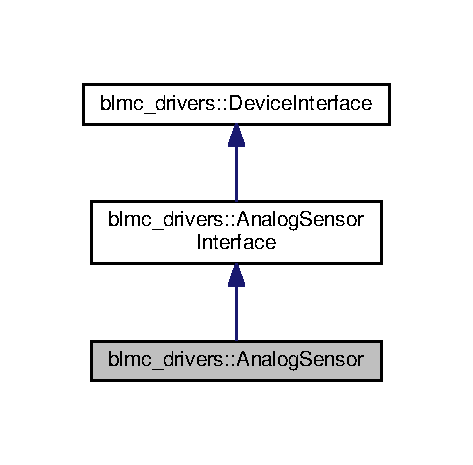
\includegraphics[width=227pt]{classblmc__drivers_1_1AnalogSensor__inherit__graph}
\end{center}
\end{figure}


Collaboration diagram for blmc\+\_\+drivers\+:\+:Analog\+Sensor\+:
\nopagebreak
\begin{figure}[H]
\begin{center}
\leavevmode
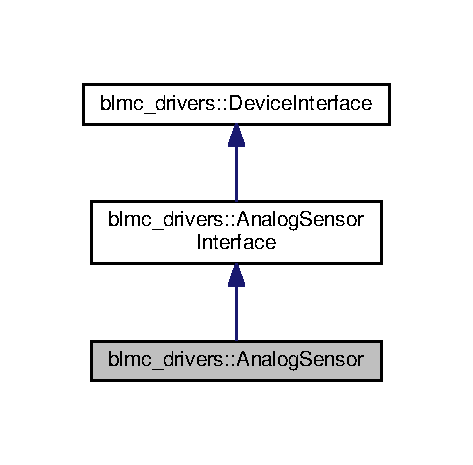
\includegraphics[width=227pt]{classblmc__drivers_1_1AnalogSensor__coll__graph}
\end{center}
\end{figure}
\subsection*{Public Member Functions}
\begin{DoxyCompactItemize}
\item 
\hyperlink{classblmc__drivers_1_1AnalogSensor_a3107ba6bba78d46e126ffc74c88f5a69}{Analog\+Sensor} (std\+::shared\+\_\+ptr$<$ \hyperlink{classblmc__drivers_1_1MotorBoardInterface}{Motor\+Board\+Interface} $>$ board, bool sensor\+\_\+id)
\begin{DoxyCompactList}\small\item\em Construct a new \hyperlink{classblmc__drivers_1_1AnalogSensor}{Analog\+Sensor} object. \end{DoxyCompactList}\item 
virtual std\+::shared\+\_\+ptr$<$ const \hyperlink{classblmc__drivers_1_1AnalogSensorInterface_a4e4a853aa044b7d3afbaa3fe20477602}{Scalar\+Timeseries} $>$ \hyperlink{classblmc__drivers_1_1AnalogSensor_ae6edd73f6625a940a05042bef9a4c264}{get\+\_\+measurement} () const 
\begin{DoxyCompactList}\small\item\em Get the measurement object which is the list of time stamped data. \end{DoxyCompactList}\end{DoxyCompactItemize}
\subsection*{Private Attributes}
\begin{DoxyCompactItemize}
\item 
std\+::shared\+\_\+ptr$<$ \hyperlink{classblmc__drivers_1_1MotorBoardInterface}{Motor\+Board\+Interface} $>$ \hyperlink{classblmc__drivers_1_1AnalogSensor_aba119f9ef91766777134c6df9f687b7c}{board\+\_\+}\hypertarget{classblmc__drivers_1_1AnalogSensor_aba119f9ef91766777134c6df9f687b7c}{}\label{classblmc__drivers_1_1AnalogSensor_aba119f9ef91766777134c6df9f687b7c}

\begin{DoxyCompactList}\small\item\em board\+\_\+ is the measurement object, it caontains the list of the timed stamped data \end{DoxyCompactList}\item 
size\+\_\+t \hyperlink{classblmc__drivers_1_1AnalogSensor_aaa093ae58c295f8da66bc23d1f241095}{sensor\+\_\+id\+\_\+}\hypertarget{classblmc__drivers_1_1AnalogSensor_aaa093ae58c295f8da66bc23d1f241095}{}\label{classblmc__drivers_1_1AnalogSensor_aaa093ae58c295f8da66bc23d1f241095}

\begin{DoxyCompactList}\small\item\em sensor\+\_\+id\+\_\+ is the identification number of the sensor on the control board, for now it is either 0 or 1 \end{DoxyCompactList}\end{DoxyCompactItemize}
\subsection*{Additional Inherited Members}


\subsection{Detailed Description}
\hyperlink{classblmc__drivers_1_1AnalogSensor}{Analog\+Sensor} class is the implementation of the above interface. 

\subsection{Constructor \& Destructor Documentation}
\index{blmc\+\_\+drivers\+::\+Analog\+Sensor@{blmc\+\_\+drivers\+::\+Analog\+Sensor}!Analog\+Sensor@{Analog\+Sensor}}
\index{Analog\+Sensor@{Analog\+Sensor}!blmc\+\_\+drivers\+::\+Analog\+Sensor@{blmc\+\_\+drivers\+::\+Analog\+Sensor}}
\subsubsection[{\texorpdfstring{Analog\+Sensor(std\+::shared\+\_\+ptr$<$ Motor\+Board\+Interface $>$ board, bool sensor\+\_\+id)}{AnalogSensor(std::shared_ptr< MotorBoardInterface > board, bool sensor_id)}}]{\setlength{\rightskip}{0pt plus 5cm}blmc\+\_\+drivers\+::\+Analog\+Sensor\+::\+Analog\+Sensor (
\begin{DoxyParamCaption}
\item[{std\+::shared\+\_\+ptr$<$ {\bf Motor\+Board\+Interface} $>$}]{board, }
\item[{bool}]{sensor\+\_\+id}
\end{DoxyParamCaption}
)}\hypertarget{classblmc__drivers_1_1AnalogSensor_a3107ba6bba78d46e126ffc74c88f5a69}{}\label{classblmc__drivers_1_1AnalogSensor_a3107ba6bba78d46e126ffc74c88f5a69}


Construct a new \hyperlink{classblmc__drivers_1_1AnalogSensor}{Analog\+Sensor} object. 


\begin{DoxyParams}{Parameters}
{\em board} & is a motor board which gives access to the motor sensors (position, velocity, current, etc) and to the motor cotrols. \\
\hline
{\em sensor\+\_\+id} & is the id of the sensor on the control board \\
\hline
\end{DoxyParams}


\subsection{Member Function Documentation}
\index{blmc\+\_\+drivers\+::\+Analog\+Sensor@{blmc\+\_\+drivers\+::\+Analog\+Sensor}!get\+\_\+measurement@{get\+\_\+measurement}}
\index{get\+\_\+measurement@{get\+\_\+measurement}!blmc\+\_\+drivers\+::\+Analog\+Sensor@{blmc\+\_\+drivers\+::\+Analog\+Sensor}}
\subsubsection[{\texorpdfstring{get\+\_\+measurement() const }{get_measurement() const }}]{\setlength{\rightskip}{0pt plus 5cm}std\+::shared\+\_\+ptr$<$ const {\bf Analog\+Sensor\+Interface\+::\+Scalar\+Timeseries} $>$ blmc\+\_\+drivers\+::\+Analog\+Sensor\+::get\+\_\+measurement (
\begin{DoxyParamCaption}
{}
\end{DoxyParamCaption}
) const\hspace{0.3cm}{\ttfamily [virtual]}}\hypertarget{classblmc__drivers_1_1AnalogSensor_ae6edd73f6625a940a05042bef9a4c264}{}\label{classblmc__drivers_1_1AnalogSensor_ae6edd73f6625a940a05042bef9a4c264}


Get the measurement object which is the list of time stamped data. 

\begin{DoxyReturn}{Returns}
std\+::shared\+\_\+ptr$<$const Scalar\+Timeseries$>$ which is a pointer to the a list of time stamped data 
\end{DoxyReturn}


Implements \hyperlink{classblmc__drivers_1_1AnalogSensorInterface_afd694f79c9fec5a35984d468f59f315c}{blmc\+\_\+drivers\+::\+Analog\+Sensor\+Interface}.



The documentation for this class was generated from the following files\+:\begin{DoxyCompactItemize}
\item 
include/blmc\+\_\+drivers/devices/\hyperlink{analog__sensor_8hpp}{analog\+\_\+sensor.\+hpp}\item 
src/\hyperlink{analog__sensors_8cpp}{analog\+\_\+sensors.\+cpp}\end{DoxyCompactItemize}

\hypertarget{classblmc__drivers_1_1AnalogSensorInterface}{}\section{blmc\+\_\+drivers\+:\+:Analog\+Sensor\+Interface Class Reference}
\label{classblmc__drivers_1_1AnalogSensorInterface}\index{blmc\+\_\+drivers\+::\+Analog\+Sensor\+Interface@{blmc\+\_\+drivers\+::\+Analog\+Sensor\+Interface}}


\hyperlink{classblmc__drivers_1_1AnalogSensorInterface}{Analog\+Sensor\+Interface} class is a simple abstract interface for using blmc analog measurements.  




{\ttfamily \#include $<$analog\+\_\+sensor.\+hpp$>$}



Inheritance diagram for blmc\+\_\+drivers\+:\+:Analog\+Sensor\+Interface\+:
\nopagebreak
\begin{figure}[H]
\begin{center}
\leavevmode
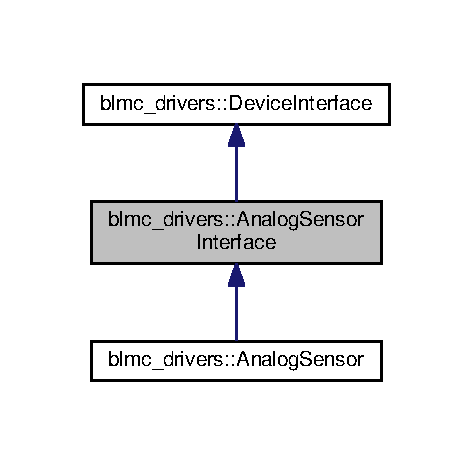
\includegraphics[width=227pt]{classblmc__drivers_1_1AnalogSensorInterface__inherit__graph}
\end{center}
\end{figure}


Collaboration diagram for blmc\+\_\+drivers\+:\+:Analog\+Sensor\+Interface\+:
\nopagebreak
\begin{figure}[H]
\begin{center}
\leavevmode
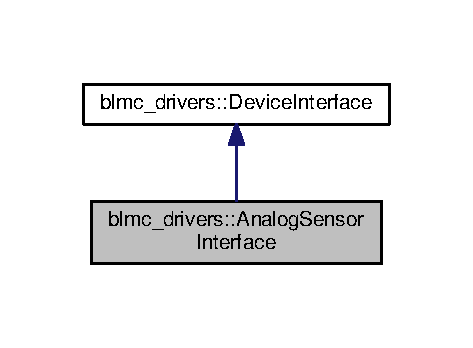
\includegraphics[width=227pt]{classblmc__drivers_1_1AnalogSensorInterface__coll__graph}
\end{center}
\end{figure}
\subsection*{Public Types}
\begin{DoxyCompactItemize}
\item 
typedef real\+\_\+time\+\_\+tools\+::\+Threadsafe\+Timeseries$<$ double $>$ \hyperlink{classblmc__drivers_1_1AnalogSensorInterface_a4e4a853aa044b7d3afbaa3fe20477602}{Scalar\+Timeseries}\hypertarget{classblmc__drivers_1_1AnalogSensorInterface_a4e4a853aa044b7d3afbaa3fe20477602}{}\label{classblmc__drivers_1_1AnalogSensorInterface_a4e4a853aa044b7d3afbaa3fe20477602}

\begin{DoxyCompactList}\small\item\em This is just a short cut for the time series types. \end{DoxyCompactList}\end{DoxyCompactItemize}
\subsection*{Public Member Functions}
\begin{DoxyCompactItemize}
\item 
virtual std\+::shared\+\_\+ptr$<$ const \hyperlink{classblmc__drivers_1_1AnalogSensorInterface_a4e4a853aa044b7d3afbaa3fe20477602}{Scalar\+Timeseries} $>$ \hyperlink{classblmc__drivers_1_1AnalogSensorInterface_afd694f79c9fec5a35984d468f59f315c}{get\+\_\+measurement} () const =0
\begin{DoxyCompactList}\small\item\em Get the measurement object which is the list of time stamped data. \end{DoxyCompactList}\item 
virtual \hyperlink{classblmc__drivers_1_1AnalogSensorInterface_a809cd9b86ae1cb9119a2ad025163afa9}{$\sim$\+Analog\+Sensor\+Interface} ()
\begin{DoxyCompactList}\small\item\em Destroy the \hyperlink{classblmc__drivers_1_1AnalogSensorInterface}{Analog\+Sensor\+Interface} object. \end{DoxyCompactList}\end{DoxyCompactItemize}


\subsection{Detailed Description}
\hyperlink{classblmc__drivers_1_1AnalogSensorInterface}{Analog\+Sensor\+Interface} class is a simple abstract interface for using blmc analog measurements. 

\subsection{Constructor \& Destructor Documentation}
\index{blmc\+\_\+drivers\+::\+Analog\+Sensor\+Interface@{blmc\+\_\+drivers\+::\+Analog\+Sensor\+Interface}!````~Analog\+Sensor\+Interface@{$\sim$\+Analog\+Sensor\+Interface}}
\index{````~Analog\+Sensor\+Interface@{$\sim$\+Analog\+Sensor\+Interface}!blmc\+\_\+drivers\+::\+Analog\+Sensor\+Interface@{blmc\+\_\+drivers\+::\+Analog\+Sensor\+Interface}}
\subsubsection[{\texorpdfstring{$\sim$\+Analog\+Sensor\+Interface()}{~AnalogSensorInterface()}}]{\setlength{\rightskip}{0pt plus 5cm}virtual blmc\+\_\+drivers\+::\+Analog\+Sensor\+Interface\+::$\sim$\+Analog\+Sensor\+Interface (
\begin{DoxyParamCaption}
{}
\end{DoxyParamCaption}
)\hspace{0.3cm}{\ttfamily [inline]}, {\ttfamily [virtual]}}\hypertarget{classblmc__drivers_1_1AnalogSensorInterface_a809cd9b86ae1cb9119a2ad025163afa9}{}\label{classblmc__drivers_1_1AnalogSensorInterface_a809cd9b86ae1cb9119a2ad025163afa9}


Destroy the \hyperlink{classblmc__drivers_1_1AnalogSensorInterface}{Analog\+Sensor\+Interface} object. 



\subsection{Member Function Documentation}
\index{blmc\+\_\+drivers\+::\+Analog\+Sensor\+Interface@{blmc\+\_\+drivers\+::\+Analog\+Sensor\+Interface}!get\+\_\+measurement@{get\+\_\+measurement}}
\index{get\+\_\+measurement@{get\+\_\+measurement}!blmc\+\_\+drivers\+::\+Analog\+Sensor\+Interface@{blmc\+\_\+drivers\+::\+Analog\+Sensor\+Interface}}
\subsubsection[{\texorpdfstring{get\+\_\+measurement() const =0}{get_measurement() const =0}}]{\setlength{\rightskip}{0pt plus 5cm}virtual std\+::shared\+\_\+ptr$<$const {\bf Scalar\+Timeseries}$>$ blmc\+\_\+drivers\+::\+Analog\+Sensor\+Interface\+::get\+\_\+measurement (
\begin{DoxyParamCaption}
{}
\end{DoxyParamCaption}
) const\hspace{0.3cm}{\ttfamily [pure virtual]}}\hypertarget{classblmc__drivers_1_1AnalogSensorInterface_afd694f79c9fec5a35984d468f59f315c}{}\label{classblmc__drivers_1_1AnalogSensorInterface_afd694f79c9fec5a35984d468f59f315c}


Get the measurement object which is the list of time stamped data. 

\begin{DoxyReturn}{Returns}
std\+::shared\+\_\+ptr$<$const Scalar\+Timeseries$>$ which is a pointer to the a list of time stamped data 
\end{DoxyReturn}


Implemented in \hyperlink{classblmc__drivers_1_1AnalogSensor_ae6edd73f6625a940a05042bef9a4c264}{blmc\+\_\+drivers\+::\+Analog\+Sensor}.



The documentation for this class was generated from the following file\+:\begin{DoxyCompactItemize}
\item 
include/blmc\+\_\+drivers/devices/\hyperlink{analog__sensor_8hpp}{analog\+\_\+sensor.\+hpp}\end{DoxyCompactItemize}

\hypertarget{classblmc__drivers_1_1CanBus}{}\section{blmc\+\_\+drivers\+:\+:Can\+Bus Class Reference}
\label{classblmc__drivers_1_1CanBus}\index{blmc\+\_\+drivers\+::\+Can\+Bus@{blmc\+\_\+drivers\+::\+Can\+Bus}}


\hyperlink{classblmc__drivers_1_1CanBus}{Can\+Bus} is the implementation of the \hyperlink{classblmc__drivers_1_1CanBusInterface}{Can\+Bus\+Interface}.  




{\ttfamily \#include $<$can\+\_\+bus.\+hpp$>$}



Inheritance diagram for blmc\+\_\+drivers\+:\+:Can\+Bus\+:
\nopagebreak
\begin{figure}[H]
\begin{center}
\leavevmode
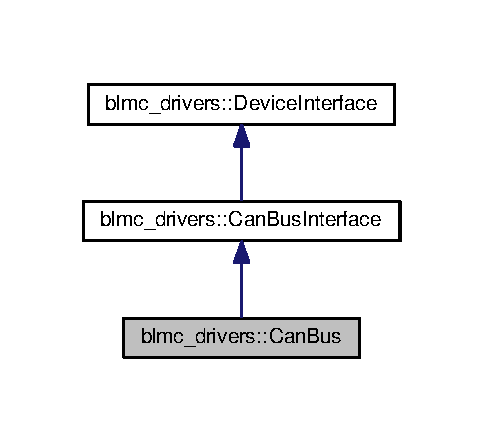
\includegraphics[width=232pt]{classblmc__drivers_1_1CanBus__inherit__graph}
\end{center}
\end{figure}


Collaboration diagram for blmc\+\_\+drivers\+:\+:Can\+Bus\+:
\nopagebreak
\begin{figure}[H]
\begin{center}
\leavevmode
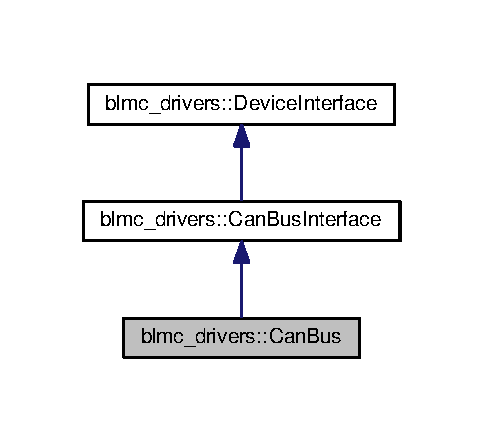
\includegraphics[width=232pt]{classblmc__drivers_1_1CanBus__coll__graph}
\end{center}
\end{figure}
\subsection*{Public Member Functions}
\begin{DoxyCompactItemize}
\item 
\hyperlink{classblmc__drivers_1_1CanBus_a7d376f1ebd6dd8bc3299f6fc9f3d42c6}{Can\+Bus} (const std\+::string \&can\+\_\+interface\+\_\+name, const size\+\_\+t \&history\+\_\+length=1000)
\begin{DoxyCompactList}\small\item\em Construct a new \hyperlink{classblmc__drivers_1_1CanBus}{Can\+Bus} object. \end{DoxyCompactList}\item 
virtual \hyperlink{classblmc__drivers_1_1CanBus_aa79afdda8d7f28ea63d32bf1a5a0f196}{$\sim$\+Can\+Bus} ()\hypertarget{classblmc__drivers_1_1CanBus_aa79afdda8d7f28ea63d32bf1a5a0f196}{}\label{classblmc__drivers_1_1CanBus_aa79afdda8d7f28ea63d32bf1a5a0f196}

\begin{DoxyCompactList}\small\item\em Destroy the \hyperlink{classblmc__drivers_1_1CanBus}{Can\+Bus} object. \end{DoxyCompactList}\item 
std\+::shared\+\_\+ptr$<$ const \hyperlink{classblmc__drivers_1_1CanBusInterface_a2da2627c961927f48359ae7d7e1aa4da}{Canframe\+Timeseries} $>$ \hyperlink{classblmc__drivers_1_1CanBus_a4504e6b71cba6d71de33925f9d401cb1}{get\+\_\+output\+\_\+frame} () const 
\begin{DoxyCompactList}\small\item\em Getters. \end{DoxyCompactList}\item 
virtual std\+::shared\+\_\+ptr$<$ const \hyperlink{classblmc__drivers_1_1CanBusInterface_a2da2627c961927f48359ae7d7e1aa4da}{Canframe\+Timeseries} $>$ \hyperlink{classblmc__drivers_1_1CanBus_a5b9282bc65bff196e6d6b393fbdc5891}{get\+\_\+input\+\_\+frame} ()
\begin{DoxyCompactList}\small\item\em Get the input frame. \end{DoxyCompactList}\item 
virtual std\+::shared\+\_\+ptr$<$ const \hyperlink{classblmc__drivers_1_1CanBusInterface_a2da2627c961927f48359ae7d7e1aa4da}{Canframe\+Timeseries} $>$ \hyperlink{classblmc__drivers_1_1CanBus_a862e9898a6607ac2e00e712c30e7f348}{get\+\_\+sent\+\_\+input\+\_\+frame} ()
\begin{DoxyCompactList}\small\item\em Get the input frame thas has been sent. \end{DoxyCompactList}\item 
virtual void \hyperlink{classblmc__drivers_1_1CanBus_ae4887644960c0a92fc82f8bdffbe9c48}{set\+\_\+input\+\_\+frame} (const \hyperlink{classblmc__drivers_1_1CanBusFrame}{Can\+Bus\+Frame} \&input\+\_\+frame)
\begin{DoxyCompactList}\small\item\em Setters. \end{DoxyCompactList}\item 
virtual void \hyperlink{classblmc__drivers_1_1CanBus_acf90b96ca5727f9ecb328ce20d7a2cbc}{send\+\_\+if\+\_\+input\+\_\+changed} ()
\begin{DoxyCompactList}\small\item\em Sender. \end{DoxyCompactList}\end{DoxyCompactItemize}
\subsection*{Private Member Functions}
\begin{DoxyCompactItemize}
\item 
void \hyperlink{classblmc__drivers_1_1CanBus_a65042f6d32e30c7c367d7e5780856a60}{loop} ()\hypertarget{classblmc__drivers_1_1CanBus_a65042f6d32e30c7c367d7e5780856a60}{}\label{classblmc__drivers_1_1CanBus_a65042f6d32e30c7c367d7e5780856a60}

\begin{DoxyCompactList}\small\item\em Execute the communication loop with the can bus. \end{DoxyCompactList}\item 
void \hyperlink{classblmc__drivers_1_1CanBus_ae445662e791d0b6149289d9df39e1ea0}{send\+\_\+frame} (const \hyperlink{classblmc__drivers_1_1CanBusFrame}{Can\+Bus\+Frame} \&unstamped\+\_\+can\+\_\+frame)
\begin{DoxyCompactList}\small\item\em Send input data. \end{DoxyCompactList}\item 
\hyperlink{classblmc__drivers_1_1CanBusFrame}{Can\+Bus\+Frame} \hyperlink{classblmc__drivers_1_1CanBus_ada25ff1dcd774666f423b23d4de664ea}{receive\+\_\+frame} ()
\begin{DoxyCompactList}\small\item\em Get the output frame from the bus. \end{DoxyCompactList}\item 
\hyperlink{classblmc__drivers_1_1CanBusConnection}{Can\+Bus\+Connection} \hyperlink{classblmc__drivers_1_1CanBus_a86826b4acc0833e041e6ea02824f8d48}{setup\+\_\+can} (std\+::string name, uint32\+\_\+t err\+\_\+mask)
\begin{DoxyCompactList}\small\item\em Setup and initialize the \hyperlink{classblmc__drivers_1_1CanBus}{Can\+Bus} object. \end{DoxyCompactList}\end{DoxyCompactItemize}
\subsection*{Static Private Member Functions}
\begin{DoxyCompactItemize}
\item 
static T\+H\+R\+E\+A\+D\+\_\+\+F\+U\+N\+C\+T\+I\+O\+N\+\_\+\+R\+E\+T\+U\+R\+N\+\_\+\+T\+Y\+PE \hyperlink{classblmc__drivers_1_1CanBus_ab39625e5a1fea7d25d0967b4a48de0b4}{loop} (void $\ast$instance\+\_\+pointer)
\begin{DoxyCompactList}\small\item\em private attributes and methods \end{DoxyCompactList}\end{DoxyCompactItemize}
\subsection*{Private Attributes}
\begin{DoxyCompactItemize}
\item 
real\+\_\+time\+\_\+tools\+::\+Singletype\+Threadsafe\+Object$<$ \hyperlink{classblmc__drivers_1_1CanBusConnection}{Can\+Bus\+Connection}, 1 $>$ \hyperlink{classblmc__drivers_1_1CanBus_a996c9b1bc46071b2d002de38d6e9f781}{can\+\_\+connection\+\_\+}
\begin{DoxyCompactList}\small\item\em Attributes. \end{DoxyCompactList}\item 
std\+::shared\+\_\+ptr$<$ real\+\_\+time\+\_\+tools\+::\+Threadsafe\+Timeseries$<$ \hyperlink{classblmc__drivers_1_1CanBusFrame}{Can\+Bus\+Frame} $>$ $>$ \hyperlink{classblmc__drivers_1_1CanBus_ab09707f2c5f6cb7eb98f82e8e190d3c4}{input\+\_\+}\hypertarget{classblmc__drivers_1_1CanBus_ab09707f2c5f6cb7eb98f82e8e190d3c4}{}\label{classblmc__drivers_1_1CanBus_ab09707f2c5f6cb7eb98f82e8e190d3c4}

\begin{DoxyCompactList}\small\item\em input\+\_\+ is a list of time stamped frame to be send to the can network. \end{DoxyCompactList}\item 
std\+::shared\+\_\+ptr$<$ real\+\_\+time\+\_\+tools\+::\+Threadsafe\+Timeseries$<$ \hyperlink{classblmc__drivers_1_1CanBusFrame}{Can\+Bus\+Frame} $>$ $>$ \hyperlink{classblmc__drivers_1_1CanBus_ae1ecf491b819c83eb999bb9cdde6fb21}{sent\+\_\+input\+\_\+}\hypertarget{classblmc__drivers_1_1CanBus_ae1ecf491b819c83eb999bb9cdde6fb21}{}\label{classblmc__drivers_1_1CanBus_ae1ecf491b819c83eb999bb9cdde6fb21}

\begin{DoxyCompactList}\small\item\em sent\+\_\+inupt\+\_\+ is the list of the input already sent to the network. \end{DoxyCompactList}\item 
std\+::shared\+\_\+ptr$<$ real\+\_\+time\+\_\+tools\+::\+Threadsafe\+Timeseries$<$ \hyperlink{classblmc__drivers_1_1CanBusFrame}{Can\+Bus\+Frame} $>$ $>$ \hyperlink{classblmc__drivers_1_1CanBus_ad9802d502698f202f9842a0c00372931}{output\+\_\+}\hypertarget{classblmc__drivers_1_1CanBus_ad9802d502698f202f9842a0c00372931}{}\label{classblmc__drivers_1_1CanBus_ad9802d502698f202f9842a0c00372931}

\begin{DoxyCompactList}\small\item\em output\+\_\+ is the list of the frames received from the can network. \end{DoxyCompactList}\item 
bool \hyperlink{classblmc__drivers_1_1CanBus_a85c9d5d9c6413c6871d48a247660ac20}{is\+\_\+loop\+\_\+active\+\_\+}\hypertarget{classblmc__drivers_1_1CanBus_a85c9d5d9c6413c6871d48a247660ac20}{}\label{classblmc__drivers_1_1CanBus_a85c9d5d9c6413c6871d48a247660ac20}

\begin{DoxyCompactList}\small\item\em This boolean makes sure that the loop is not active upon destruction of the current object. \end{DoxyCompactList}\item 
real\+\_\+time\+\_\+tools\+::\+Real\+Time\+Thread \hyperlink{classblmc__drivers_1_1CanBus_a906baf827eff3c2850728478764a4759}{rt\+\_\+thread\+\_\+}\hypertarget{classblmc__drivers_1_1CanBus_a906baf827eff3c2850728478764a4759}{}\label{classblmc__drivers_1_1CanBus_a906baf827eff3c2850728478764a4759}

\begin{DoxyCompactList}\small\item\em rt\+\_\+thread\+\_\+ is the thread object allowing us to spawn real-\/time threads. \end{DoxyCompactList}\item 
std\+::string \hyperlink{classblmc__drivers_1_1CanBus_aef341b0b36d3f02087047b5234ccbf79}{log\+\_\+dir\+\_\+}\hypertarget{classblmc__drivers_1_1CanBus_aef341b0b36d3f02087047b5234ccbf79}{}\label{classblmc__drivers_1_1CanBus_aef341b0b36d3f02087047b5234ccbf79}

\begin{DoxyCompactList}\small\item\em Log directory. \end{DoxyCompactList}\item 
std\+::string \hyperlink{classblmc__drivers_1_1CanBus_aa726bd0d63a783d2a3cc02e2ef9c929b}{name\+\_\+}\hypertarget{classblmc__drivers_1_1CanBus_aa726bd0d63a783d2a3cc02e2ef9c929b}{}\label{classblmc__drivers_1_1CanBus_aa726bd0d63a783d2a3cc02e2ef9c929b}

\begin{DoxyCompactList}\small\item\em time\+\_\+log\+\_\+name is the name of the loggin \end{DoxyCompactList}\end{DoxyCompactItemize}
\subsection*{Additional Inherited Members}


\subsection{Detailed Description}
\hyperlink{classblmc__drivers_1_1CanBus}{Can\+Bus} is the implementation of the \hyperlink{classblmc__drivers_1_1CanBusInterface}{Can\+Bus\+Interface}. 

\subsection{Constructor \& Destructor Documentation}
\index{blmc\+\_\+drivers\+::\+Can\+Bus@{blmc\+\_\+drivers\+::\+Can\+Bus}!Can\+Bus@{Can\+Bus}}
\index{Can\+Bus@{Can\+Bus}!blmc\+\_\+drivers\+::\+Can\+Bus@{blmc\+\_\+drivers\+::\+Can\+Bus}}
\subsubsection[{\texorpdfstring{Can\+Bus(const std\+::string \&can\+\_\+interface\+\_\+name, const size\+\_\+t \&history\+\_\+length=1000)}{CanBus(const std::string &can_interface_name, const size_t &history_length=1000)}}]{\setlength{\rightskip}{0pt plus 5cm}blmc\+\_\+drivers\+::\+Can\+Bus\+::\+Can\+Bus (
\begin{DoxyParamCaption}
\item[{const std\+::string \&}]{can\+\_\+interface\+\_\+name, }
\item[{const size\+\_\+t \&}]{history\+\_\+length = {\ttfamily 1000}}
\end{DoxyParamCaption}
)}\hypertarget{classblmc__drivers_1_1CanBus_a7d376f1ebd6dd8bc3299f6fc9f3d42c6}{}\label{classblmc__drivers_1_1CanBus_a7d376f1ebd6dd8bc3299f6fc9f3d42c6}


Construct a new \hyperlink{classblmc__drivers_1_1CanBus}{Can\+Bus} object. 


\begin{DoxyParams}{Parameters}
{\em can\+\_\+interface\+\_\+name} & \\
\hline
{\em history\+\_\+length} & \\
\hline
\end{DoxyParams}


\subsection{Member Function Documentation}
\index{blmc\+\_\+drivers\+::\+Can\+Bus@{blmc\+\_\+drivers\+::\+Can\+Bus}!get\+\_\+input\+\_\+frame@{get\+\_\+input\+\_\+frame}}
\index{get\+\_\+input\+\_\+frame@{get\+\_\+input\+\_\+frame}!blmc\+\_\+drivers\+::\+Can\+Bus@{blmc\+\_\+drivers\+::\+Can\+Bus}}
\subsubsection[{\texorpdfstring{get\+\_\+input\+\_\+frame()}{get_input_frame()}}]{\setlength{\rightskip}{0pt plus 5cm}virtual std\+::shared\+\_\+ptr$<$const {\bf Canframe\+Timeseries}$>$ blmc\+\_\+drivers\+::\+Can\+Bus\+::get\+\_\+input\+\_\+frame (
\begin{DoxyParamCaption}
{}
\end{DoxyParamCaption}
)\hspace{0.3cm}{\ttfamily [inline]}, {\ttfamily [virtual]}}\hypertarget{classblmc__drivers_1_1CanBus_a5b9282bc65bff196e6d6b393fbdc5891}{}\label{classblmc__drivers_1_1CanBus_a5b9282bc65bff196e6d6b393fbdc5891}


Get the input frame. 

\begin{DoxyReturn}{Returns}
std\+::shared\+\_\+ptr$<$const Canframe\+Timeseries$>$ 
\end{DoxyReturn}


Implements \hyperlink{classblmc__drivers_1_1CanBusInterface_a40b62805094dc0a454695a988ab0d403}{blmc\+\_\+drivers\+::\+Can\+Bus\+Interface}.

\index{blmc\+\_\+drivers\+::\+Can\+Bus@{blmc\+\_\+drivers\+::\+Can\+Bus}!get\+\_\+output\+\_\+frame@{get\+\_\+output\+\_\+frame}}
\index{get\+\_\+output\+\_\+frame@{get\+\_\+output\+\_\+frame}!blmc\+\_\+drivers\+::\+Can\+Bus@{blmc\+\_\+drivers\+::\+Can\+Bus}}
\subsubsection[{\texorpdfstring{get\+\_\+output\+\_\+frame() const }{get_output_frame() const }}]{\setlength{\rightskip}{0pt plus 5cm}std\+::shared\+\_\+ptr$<$const {\bf Canframe\+Timeseries}$>$ blmc\+\_\+drivers\+::\+Can\+Bus\+::get\+\_\+output\+\_\+frame (
\begin{DoxyParamCaption}
{}
\end{DoxyParamCaption}
) const\hspace{0.3cm}{\ttfamily [inline]}, {\ttfamily [virtual]}}\hypertarget{classblmc__drivers_1_1CanBus_a4504e6b71cba6d71de33925f9d401cb1}{}\label{classblmc__drivers_1_1CanBus_a4504e6b71cba6d71de33925f9d401cb1}


Getters. 

Get the output frame

\begin{DoxyReturn}{Returns}
std\+::shared\+\_\+ptr$<$const Canframe\+Timeseries$>$ 
\end{DoxyReturn}


Implements \hyperlink{classblmc__drivers_1_1CanBusInterface_ac169b1c119b707d2946a999b81fb5a46}{blmc\+\_\+drivers\+::\+Can\+Bus\+Interface}.

\index{blmc\+\_\+drivers\+::\+Can\+Bus@{blmc\+\_\+drivers\+::\+Can\+Bus}!get\+\_\+sent\+\_\+input\+\_\+frame@{get\+\_\+sent\+\_\+input\+\_\+frame}}
\index{get\+\_\+sent\+\_\+input\+\_\+frame@{get\+\_\+sent\+\_\+input\+\_\+frame}!blmc\+\_\+drivers\+::\+Can\+Bus@{blmc\+\_\+drivers\+::\+Can\+Bus}}
\subsubsection[{\texorpdfstring{get\+\_\+sent\+\_\+input\+\_\+frame()}{get_sent_input_frame()}}]{\setlength{\rightskip}{0pt plus 5cm}virtual std\+::shared\+\_\+ptr$<$const {\bf Canframe\+Timeseries}$>$ blmc\+\_\+drivers\+::\+Can\+Bus\+::get\+\_\+sent\+\_\+input\+\_\+frame (
\begin{DoxyParamCaption}
{}
\end{DoxyParamCaption}
)\hspace{0.3cm}{\ttfamily [inline]}, {\ttfamily [virtual]}}\hypertarget{classblmc__drivers_1_1CanBus_a862e9898a6607ac2e00e712c30e7f348}{}\label{classblmc__drivers_1_1CanBus_a862e9898a6607ac2e00e712c30e7f348}


Get the input frame thas has been sent. 

\begin{DoxyReturn}{Returns}
std\+::shared\+\_\+ptr$<$const Canframe\+Timeseries$>$ 
\end{DoxyReturn}


Implements \hyperlink{classblmc__drivers_1_1CanBusInterface_aca7e703983284a09c497c8182c0684d5}{blmc\+\_\+drivers\+::\+Can\+Bus\+Interface}.

\index{blmc\+\_\+drivers\+::\+Can\+Bus@{blmc\+\_\+drivers\+::\+Can\+Bus}!loop@{loop}}
\index{loop@{loop}!blmc\+\_\+drivers\+::\+Can\+Bus@{blmc\+\_\+drivers\+::\+Can\+Bus}}
\subsubsection[{\texorpdfstring{loop(void $\ast$instance\+\_\+pointer)}{loop(void *instance_pointer)}}]{\setlength{\rightskip}{0pt plus 5cm}static T\+H\+R\+E\+A\+D\+\_\+\+F\+U\+N\+C\+T\+I\+O\+N\+\_\+\+R\+E\+T\+U\+R\+N\+\_\+\+T\+Y\+PE blmc\+\_\+drivers\+::\+Can\+Bus\+::loop (
\begin{DoxyParamCaption}
\item[{void $\ast$}]{instance\+\_\+pointer}
\end{DoxyParamCaption}
)\hspace{0.3cm}{\ttfamily [inline]}, {\ttfamily [static]}, {\ttfamily [private]}}\hypertarget{classblmc__drivers_1_1CanBus_ab39625e5a1fea7d25d0967b4a48de0b4}{}\label{classblmc__drivers_1_1CanBus_ab39625e5a1fea7d25d0967b4a48de0b4}


private attributes and methods 

This function is an helper that allows us to launch real-\/time thread in xenaomai, ubunt, or rt-\/preempt seemlessly.


\begin{DoxyParams}{Parameters}
{\em instance\+\_\+pointer} & \\
\hline
\end{DoxyParams}
\begin{DoxyReturn}{Returns}
T\+H\+R\+E\+A\+D\+\_\+\+F\+U\+N\+C\+T\+I\+O\+N\+\_\+\+R\+E\+T\+U\+R\+N\+\_\+\+T\+Y\+PE (is void or void$\ast$ depending on the OS. 
\end{DoxyReturn}
\index{blmc\+\_\+drivers\+::\+Can\+Bus@{blmc\+\_\+drivers\+::\+Can\+Bus}!receive\+\_\+frame@{receive\+\_\+frame}}
\index{receive\+\_\+frame@{receive\+\_\+frame}!blmc\+\_\+drivers\+::\+Can\+Bus@{blmc\+\_\+drivers\+::\+Can\+Bus}}
\subsubsection[{\texorpdfstring{receive\+\_\+frame()}{receive_frame()}}]{\setlength{\rightskip}{0pt plus 5cm}{\bf Can\+Bus\+Frame} blmc\+\_\+drivers\+::\+Can\+Bus\+::receive\+\_\+frame (
\begin{DoxyParamCaption}
{}
\end{DoxyParamCaption}
)\hspace{0.3cm}{\ttfamily [private]}}\hypertarget{classblmc__drivers_1_1CanBus_ada25ff1dcd774666f423b23d4de664ea}{}\label{classblmc__drivers_1_1CanBus_ada25ff1dcd774666f423b23d4de664ea}


Get the output frame from the bus. 

\begin{DoxyReturn}{Returns}
\hyperlink{classblmc__drivers_1_1CanBusFrame}{Can\+Bus\+Frame} is the output frame data. 
\end{DoxyReturn}
\index{blmc\+\_\+drivers\+::\+Can\+Bus@{blmc\+\_\+drivers\+::\+Can\+Bus}!send\+\_\+frame@{send\+\_\+frame}}
\index{send\+\_\+frame@{send\+\_\+frame}!blmc\+\_\+drivers\+::\+Can\+Bus@{blmc\+\_\+drivers\+::\+Can\+Bus}}
\subsubsection[{\texorpdfstring{send\+\_\+frame(const Can\+Bus\+Frame \&unstamped\+\_\+can\+\_\+frame)}{send_frame(const CanBusFrame &unstamped_can_frame)}}]{\setlength{\rightskip}{0pt plus 5cm}void blmc\+\_\+drivers\+::\+Can\+Bus\+::send\+\_\+frame (
\begin{DoxyParamCaption}
\item[{const {\bf Can\+Bus\+Frame} \&}]{unstamped\+\_\+can\+\_\+frame}
\end{DoxyParamCaption}
)\hspace{0.3cm}{\ttfamily [private]}}\hypertarget{classblmc__drivers_1_1CanBus_ae445662e791d0b6149289d9df39e1ea0}{}\label{classblmc__drivers_1_1CanBus_ae445662e791d0b6149289d9df39e1ea0}


Send input data. 


\begin{DoxyParams}{Parameters}
{\em unstamped\+\_\+can\+\_\+frame} & is a frame without id nor time. \\
\hline
\end{DoxyParams}
\index{blmc\+\_\+drivers\+::\+Can\+Bus@{blmc\+\_\+drivers\+::\+Can\+Bus}!send\+\_\+if\+\_\+input\+\_\+changed@{send\+\_\+if\+\_\+input\+\_\+changed}}
\index{send\+\_\+if\+\_\+input\+\_\+changed@{send\+\_\+if\+\_\+input\+\_\+changed}!blmc\+\_\+drivers\+::\+Can\+Bus@{blmc\+\_\+drivers\+::\+Can\+Bus}}
\subsubsection[{\texorpdfstring{send\+\_\+if\+\_\+input\+\_\+changed()}{send_if_input_changed()}}]{\setlength{\rightskip}{0pt plus 5cm}void blmc\+\_\+drivers\+::\+Can\+Bus\+::send\+\_\+if\+\_\+input\+\_\+changed (
\begin{DoxyParamCaption}
{}
\end{DoxyParamCaption}
)\hspace{0.3cm}{\ttfamily [virtual]}}\hypertarget{classblmc__drivers_1_1CanBus_acf90b96ca5727f9ecb328ce20d7a2cbc}{}\label{classblmc__drivers_1_1CanBus_acf90b96ca5727f9ecb328ce20d7a2cbc}


Sender. 

Send the queue of message to the can network 

Implements \hyperlink{classblmc__drivers_1_1CanBusInterface_aa97ce2a204aa8354b8ea62af5f3820a2}{blmc\+\_\+drivers\+::\+Can\+Bus\+Interface}.

\index{blmc\+\_\+drivers\+::\+Can\+Bus@{blmc\+\_\+drivers\+::\+Can\+Bus}!set\+\_\+input\+\_\+frame@{set\+\_\+input\+\_\+frame}}
\index{set\+\_\+input\+\_\+frame@{set\+\_\+input\+\_\+frame}!blmc\+\_\+drivers\+::\+Can\+Bus@{blmc\+\_\+drivers\+::\+Can\+Bus}}
\subsubsection[{\texorpdfstring{set\+\_\+input\+\_\+frame(const Can\+Bus\+Frame \&input\+\_\+frame)}{set_input_frame(const CanBusFrame &input_frame)}}]{\setlength{\rightskip}{0pt plus 5cm}virtual void blmc\+\_\+drivers\+::\+Can\+Bus\+::set\+\_\+input\+\_\+frame (
\begin{DoxyParamCaption}
\item[{const {\bf Can\+Bus\+Frame} \&}]{input\+\_\+frame}
\end{DoxyParamCaption}
)\hspace{0.3cm}{\ttfamily [inline]}, {\ttfamily [virtual]}}\hypertarget{classblmc__drivers_1_1CanBus_ae4887644960c0a92fc82f8bdffbe9c48}{}\label{classblmc__drivers_1_1CanBus_ae4887644960c0a92fc82f8bdffbe9c48}


Setters. 

Set the input frame


\begin{DoxyParams}{Parameters}
{\em input\+\_\+frame} & \\
\hline
\end{DoxyParams}


Implements \hyperlink{classblmc__drivers_1_1CanBusInterface_acf9305b548421e837950a0988172d57a}{blmc\+\_\+drivers\+::\+Can\+Bus\+Interface}.

\index{blmc\+\_\+drivers\+::\+Can\+Bus@{blmc\+\_\+drivers\+::\+Can\+Bus}!setup\+\_\+can@{setup\+\_\+can}}
\index{setup\+\_\+can@{setup\+\_\+can}!blmc\+\_\+drivers\+::\+Can\+Bus@{blmc\+\_\+drivers\+::\+Can\+Bus}}
\subsubsection[{\texorpdfstring{setup\+\_\+can(std\+::string name, uint32\+\_\+t err\+\_\+mask)}{setup_can(std::string name, uint32_t err_mask)}}]{\setlength{\rightskip}{0pt plus 5cm}{\bf Can\+Bus\+Connection} blmc\+\_\+drivers\+::\+Can\+Bus\+::setup\+\_\+can (
\begin{DoxyParamCaption}
\item[{std\+::string}]{name, }
\item[{uint32\+\_\+t}]{err\+\_\+mask}
\end{DoxyParamCaption}
)\hspace{0.3cm}{\ttfamily [private]}}\hypertarget{classblmc__drivers_1_1CanBus_a86826b4acc0833e041e6ea02824f8d48}{}\label{classblmc__drivers_1_1CanBus_a86826b4acc0833e041e6ea02824f8d48}


Setup and initialize the \hyperlink{classblmc__drivers_1_1CanBus}{Can\+Bus} object. 

It connects to the can bus. This method is used once in the constructor.


\begin{DoxyParams}{Parameters}
{\em name} & is the can card name. \\
\hline
{\em err\+\_\+mask,always} & used with \char`\"{}0\char`\"{} so far (T\+O\+DO\+: Manuel explain) \\
\hline
\end{DoxyParams}
\begin{DoxyReturn}{Returns}
\hyperlink{classblmc__drivers_1_1CanBusConnection}{Can\+Bus\+Connection} 
\end{DoxyReturn}


\subsection{Member Data Documentation}
\index{blmc\+\_\+drivers\+::\+Can\+Bus@{blmc\+\_\+drivers\+::\+Can\+Bus}!can\+\_\+connection\+\_\+@{can\+\_\+connection\+\_\+}}
\index{can\+\_\+connection\+\_\+@{can\+\_\+connection\+\_\+}!blmc\+\_\+drivers\+::\+Can\+Bus@{blmc\+\_\+drivers\+::\+Can\+Bus}}
\subsubsection[{\texorpdfstring{can\+\_\+connection\+\_\+}{can_connection_}}]{\setlength{\rightskip}{0pt plus 5cm}real\+\_\+time\+\_\+tools\+::\+Singletype\+Threadsafe\+Object$<${\bf Can\+Bus\+Connection}, 1$>$ blmc\+\_\+drivers\+::\+Can\+Bus\+::can\+\_\+connection\+\_\+\hspace{0.3cm}{\ttfamily [private]}}\hypertarget{classblmc__drivers_1_1CanBus_a996c9b1bc46071b2d002de38d6e9f781}{}\label{classblmc__drivers_1_1CanBus_a996c9b1bc46071b2d002de38d6e9f781}


Attributes. 

can\+\_\+connection\+\_\+ is the communication object allowing to send or receive can frames. 

The documentation for this class was generated from the following files\+:\begin{DoxyCompactItemize}
\item 
include/blmc\+\_\+drivers/devices/\hyperlink{can__bus_8hpp}{can\+\_\+bus.\+hpp}\item 
src/\hyperlink{can__bus_8cpp}{can\+\_\+bus.\+cpp}\end{DoxyCompactItemize}

\hypertarget{classblmc__drivers_1_1CanBusConnection}{}\section{blmc\+\_\+drivers\+:\+:Can\+Bus\+Connection Class Reference}
\label{classblmc__drivers_1_1CanBusConnection}\index{blmc\+\_\+drivers\+::\+Can\+Bus\+Connection@{blmc\+\_\+drivers\+::\+Can\+Bus\+Connection}}


\hyperlink{classblmc__drivers_1_1CanBusConnection}{Can\+Bus\+Connection} is a data structure that contains the hardware details for the connection between to can cards.  




{\ttfamily \#include $<$can\+\_\+bus.\+hpp$>$}

\subsection*{Public Attributes}
\begin{DoxyCompactItemize}
\item 
struct sockaddr\+\_\+can \hyperlink{classblmc__drivers_1_1CanBusConnection_a9f9e0f2d59955798cfd66ed295b76797}{send\+\_\+addr}\hypertarget{classblmc__drivers_1_1CanBusConnection_a9f9e0f2d59955798cfd66ed295b76797}{}\label{classblmc__drivers_1_1CanBusConnection_a9f9e0f2d59955798cfd66ed295b76797}

\begin{DoxyCompactList}\small\item\em send\+\_\+addr is the ip address where to send the the messages. \end{DoxyCompactList}\item 
int \hyperlink{classblmc__drivers_1_1CanBusConnection_a864cc55d83145a1a54310ef5271f67ea}{socket}\hypertarget{classblmc__drivers_1_1CanBusConnection_a864cc55d83145a1a54310ef5271f67ea}{}\label{classblmc__drivers_1_1CanBusConnection_a864cc55d83145a1a54310ef5271f67ea}

\begin{DoxyCompactList}\small\item\em socket is the port through which the messages will be processed \end{DoxyCompactList}\end{DoxyCompactItemize}


\subsection{Detailed Description}
\hyperlink{classblmc__drivers_1_1CanBusConnection}{Can\+Bus\+Connection} is a data structure that contains the hardware details for the connection between to can cards. 

The documentation for this class was generated from the following file\+:\begin{DoxyCompactItemize}
\item 
include/blmc\+\_\+drivers/devices/\hyperlink{can__bus_8hpp}{can\+\_\+bus.\+hpp}\end{DoxyCompactItemize}

\hypertarget{classblmc__drivers_1_1CanBusFrame}{}\section{blmc\+\_\+drivers\+:\+:Can\+Bus\+Frame Class Reference}
\label{classblmc__drivers_1_1CanBusFrame}\index{blmc\+\_\+drivers\+::\+Can\+Bus\+Frame@{blmc\+\_\+drivers\+::\+Can\+Bus\+Frame}}


\hyperlink{classblmc__drivers_1_1CanBusFrame}{Can\+Bus\+Frame} is a class that contains a fixed sized amount of data to be send or received via the can bus.  




{\ttfamily \#include $<$can\+\_\+bus.\+hpp$>$}

\subsection*{Public Member Functions}
\begin{DoxyCompactItemize}
\item 
void {\bfseries print} () const \hypertarget{classblmc__drivers_1_1CanBusFrame_abac5531325f1c6f7bfc2599703208869}{}\label{classblmc__drivers_1_1CanBusFrame_abac5531325f1c6f7bfc2599703208869}

\end{DoxyCompactItemize}
\subsection*{Public Attributes}
\begin{DoxyCompactItemize}
\item 
std\+::array$<$ uint8\+\_\+t, 8 $>$ \hyperlink{classblmc__drivers_1_1CanBusFrame_a1a4cd54d31de4361b003e39dfdfa4cfe}{data}\hypertarget{classblmc__drivers_1_1CanBusFrame_a1a4cd54d31de4361b003e39dfdfa4cfe}{}\label{classblmc__drivers_1_1CanBusFrame_a1a4cd54d31de4361b003e39dfdfa4cfe}

\begin{DoxyCompactList}\small\item\em data is the acutal data to be sent/received. \end{DoxyCompactList}\item 
uint8\+\_\+t \hyperlink{classblmc__drivers_1_1CanBusFrame_ab5c88f0e6fa037ace23a059a3e75b30b}{dlc}\hypertarget{classblmc__drivers_1_1CanBusFrame_ab5c88f0e6fa037ace23a059a3e75b30b}{}\label{classblmc__drivers_1_1CanBusFrame_ab5c88f0e6fa037ace23a059a3e75b30b}

\begin{DoxyCompactList}\small\item\em dlc is the size of the message. \end{DoxyCompactList}\item 
\hyperlink{os__interface_8hpp_ab9491ad99890aa9ecf1785d1edd23d64}{can\+\_\+id\+\_\+t} \hyperlink{classblmc__drivers_1_1CanBusFrame_a5d204dce9fded6502c7d51f3aabbad61}{id}\hypertarget{classblmc__drivers_1_1CanBusFrame_a5d204dce9fded6502c7d51f3aabbad61}{}\label{classblmc__drivers_1_1CanBusFrame_a5d204dce9fded6502c7d51f3aabbad61}

\begin{DoxyCompactList}\small\item\em id is the id number return by the C\+AN bus. \end{DoxyCompactList}\end{DoxyCompactItemize}


\subsection{Detailed Description}
\hyperlink{classblmc__drivers_1_1CanBusFrame}{Can\+Bus\+Frame} is a class that contains a fixed sized amount of data to be send or received via the can bus. 

The documentation for this class was generated from the following file\+:\begin{DoxyCompactItemize}
\item 
include/blmc\+\_\+drivers/devices/\hyperlink{can__bus_8hpp}{can\+\_\+bus.\+hpp}\end{DoxyCompactItemize}

\hypertarget{classblmc__drivers_1_1CanBusInterface}{}\section{blmc\+\_\+drivers\+:\+:Can\+Bus\+Interface Class Reference}
\label{classblmc__drivers_1_1CanBusInterface}\index{blmc\+\_\+drivers\+::\+Can\+Bus\+Interface@{blmc\+\_\+drivers\+::\+Can\+Bus\+Interface}}


\hyperlink{classblmc__drivers_1_1CanBusInterface}{Can\+Bus\+Interface} is an abstract class that defines an A\+PI for the communication via Can bus.  




{\ttfamily \#include $<$can\+\_\+bus.\+hpp$>$}



Inheritance diagram for blmc\+\_\+drivers\+:\+:Can\+Bus\+Interface\+:
\nopagebreak
\begin{figure}[H]
\begin{center}
\leavevmode
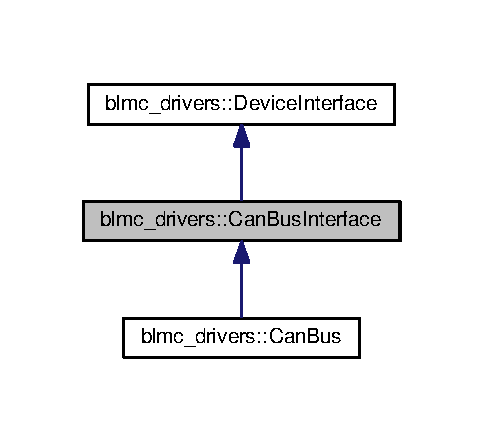
\includegraphics[width=232pt]{classblmc__drivers_1_1CanBusInterface__inherit__graph}
\end{center}
\end{figure}


Collaboration diagram for blmc\+\_\+drivers\+:\+:Can\+Bus\+Interface\+:
\nopagebreak
\begin{figure}[H]
\begin{center}
\leavevmode
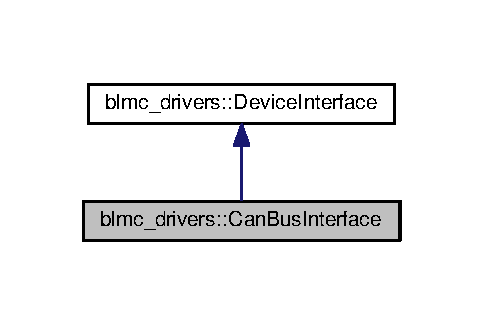
\includegraphics[width=232pt]{classblmc__drivers_1_1CanBusInterface__coll__graph}
\end{center}
\end{figure}
\subsection*{Public Types}
\begin{DoxyCompactItemize}
\item 
typedef real\+\_\+time\+\_\+tools\+::\+Threadsafe\+Timeseries$<$ \hyperlink{classblmc__drivers_1_1CanBusFrame}{Can\+Bus\+Frame} $>$ \hyperlink{classblmc__drivers_1_1CanBusInterface_a2da2627c961927f48359ae7d7e1aa4da}{Canframe\+Timeseries}\hypertarget{classblmc__drivers_1_1CanBusInterface_a2da2627c961927f48359ae7d7e1aa4da}{}\label{classblmc__drivers_1_1CanBusInterface_a2da2627c961927f48359ae7d7e1aa4da}

\begin{DoxyCompactList}\small\item\em Canframe\+Timeseries is a simple sohortcut. \end{DoxyCompactList}\end{DoxyCompactItemize}
\subsection*{Public Member Functions}
\begin{DoxyCompactItemize}
\item 
virtual \hyperlink{classblmc__drivers_1_1CanBusInterface_ac2c6e3ff3b49b04ad5f9f698eadc8690}{$\sim$\+Can\+Bus\+Interface} ()\hypertarget{classblmc__drivers_1_1CanBusInterface_ac2c6e3ff3b49b04ad5f9f698eadc8690}{}\label{classblmc__drivers_1_1CanBusInterface_ac2c6e3ff3b49b04ad5f9f698eadc8690}

\begin{DoxyCompactList}\small\item\em Destroy the \hyperlink{classblmc__drivers_1_1CanBusInterface}{Can\+Bus\+Interface} object. \end{DoxyCompactList}\item 
virtual std\+::shared\+\_\+ptr$<$ const \hyperlink{classblmc__drivers_1_1CanBusInterface_a2da2627c961927f48359ae7d7e1aa4da}{Canframe\+Timeseries} $>$ \hyperlink{classblmc__drivers_1_1CanBusInterface_ac169b1c119b707d2946a999b81fb5a46}{get\+\_\+output\+\_\+frame} () const =0
\begin{DoxyCompactList}\small\item\em getters \end{DoxyCompactList}\item 
virtual std\+::shared\+\_\+ptr$<$ const \hyperlink{classblmc__drivers_1_1CanBusInterface_a2da2627c961927f48359ae7d7e1aa4da}{Canframe\+Timeseries} $>$ \hyperlink{classblmc__drivers_1_1CanBusInterface_a40b62805094dc0a454695a988ab0d403}{get\+\_\+input\+\_\+frame} ()=0
\begin{DoxyCompactList}\small\item\em Get the input frame. \end{DoxyCompactList}\item 
virtual std\+::shared\+\_\+ptr$<$ const \hyperlink{classblmc__drivers_1_1CanBusInterface_a2da2627c961927f48359ae7d7e1aa4da}{Canframe\+Timeseries} $>$ \hyperlink{classblmc__drivers_1_1CanBusInterface_aca7e703983284a09c497c8182c0684d5}{get\+\_\+sent\+\_\+input\+\_\+frame} ()=0
\begin{DoxyCompactList}\small\item\em Get the sent input frame. \end{DoxyCompactList}\item 
virtual void \hyperlink{classblmc__drivers_1_1CanBusInterface_acf9305b548421e837950a0988172d57a}{set\+\_\+input\+\_\+frame} (const \hyperlink{classblmc__drivers_1_1CanBusFrame}{Can\+Bus\+Frame} \&input\+\_\+frame)=0
\begin{DoxyCompactList}\small\item\em setters \end{DoxyCompactList}\item 
virtual void \hyperlink{classblmc__drivers_1_1CanBusInterface_aa97ce2a204aa8354b8ea62af5f3820a2}{send\+\_\+if\+\_\+input\+\_\+changed} ()=0
\begin{DoxyCompactList}\small\item\em Sender. \end{DoxyCompactList}\end{DoxyCompactItemize}


\subsection{Detailed Description}
\hyperlink{classblmc__drivers_1_1CanBusInterface}{Can\+Bus\+Interface} is an abstract class that defines an A\+PI for the communication via Can bus. 

\subsection{Member Function Documentation}
\index{blmc\+\_\+drivers\+::\+Can\+Bus\+Interface@{blmc\+\_\+drivers\+::\+Can\+Bus\+Interface}!get\+\_\+input\+\_\+frame@{get\+\_\+input\+\_\+frame}}
\index{get\+\_\+input\+\_\+frame@{get\+\_\+input\+\_\+frame}!blmc\+\_\+drivers\+::\+Can\+Bus\+Interface@{blmc\+\_\+drivers\+::\+Can\+Bus\+Interface}}
\subsubsection[{\texorpdfstring{get\+\_\+input\+\_\+frame()=0}{get_input_frame()=0}}]{\setlength{\rightskip}{0pt plus 5cm}virtual std\+::shared\+\_\+ptr$<$const {\bf Canframe\+Timeseries}$>$ blmc\+\_\+drivers\+::\+Can\+Bus\+Interface\+::get\+\_\+input\+\_\+frame (
\begin{DoxyParamCaption}
{}
\end{DoxyParamCaption}
)\hspace{0.3cm}{\ttfamily [pure virtual]}}\hypertarget{classblmc__drivers_1_1CanBusInterface_a40b62805094dc0a454695a988ab0d403}{}\label{classblmc__drivers_1_1CanBusInterface_a40b62805094dc0a454695a988ab0d403}


Get the input frame. 

\begin{DoxyReturn}{Returns}
std\+::shared\+\_\+ptr$<$const Canframe\+Timeseries$>$ 
\end{DoxyReturn}


Implemented in \hyperlink{classblmc__drivers_1_1CanBus_a5b9282bc65bff196e6d6b393fbdc5891}{blmc\+\_\+drivers\+::\+Can\+Bus}.

\index{blmc\+\_\+drivers\+::\+Can\+Bus\+Interface@{blmc\+\_\+drivers\+::\+Can\+Bus\+Interface}!get\+\_\+output\+\_\+frame@{get\+\_\+output\+\_\+frame}}
\index{get\+\_\+output\+\_\+frame@{get\+\_\+output\+\_\+frame}!blmc\+\_\+drivers\+::\+Can\+Bus\+Interface@{blmc\+\_\+drivers\+::\+Can\+Bus\+Interface}}
\subsubsection[{\texorpdfstring{get\+\_\+output\+\_\+frame() const =0}{get_output_frame() const =0}}]{\setlength{\rightskip}{0pt plus 5cm}virtual std\+::shared\+\_\+ptr$<$const {\bf Canframe\+Timeseries}$>$ blmc\+\_\+drivers\+::\+Can\+Bus\+Interface\+::get\+\_\+output\+\_\+frame (
\begin{DoxyParamCaption}
{}
\end{DoxyParamCaption}
) const\hspace{0.3cm}{\ttfamily [pure virtual]}}\hypertarget{classblmc__drivers_1_1CanBusInterface_ac169b1c119b707d2946a999b81fb5a46}{}\label{classblmc__drivers_1_1CanBusInterface_ac169b1c119b707d2946a999b81fb5a46}


getters 

Get the output frame

\begin{DoxyReturn}{Returns}
std\+::shared\+\_\+ptr$<$const Canframe\+Timeseries$>$ 
\end{DoxyReturn}


Implemented in \hyperlink{classblmc__drivers_1_1CanBus_a4504e6b71cba6d71de33925f9d401cb1}{blmc\+\_\+drivers\+::\+Can\+Bus}.

\index{blmc\+\_\+drivers\+::\+Can\+Bus\+Interface@{blmc\+\_\+drivers\+::\+Can\+Bus\+Interface}!get\+\_\+sent\+\_\+input\+\_\+frame@{get\+\_\+sent\+\_\+input\+\_\+frame}}
\index{get\+\_\+sent\+\_\+input\+\_\+frame@{get\+\_\+sent\+\_\+input\+\_\+frame}!blmc\+\_\+drivers\+::\+Can\+Bus\+Interface@{blmc\+\_\+drivers\+::\+Can\+Bus\+Interface}}
\subsubsection[{\texorpdfstring{get\+\_\+sent\+\_\+input\+\_\+frame()=0}{get_sent_input_frame()=0}}]{\setlength{\rightskip}{0pt plus 5cm}virtual std\+::shared\+\_\+ptr$<$const {\bf Canframe\+Timeseries}$>$ blmc\+\_\+drivers\+::\+Can\+Bus\+Interface\+::get\+\_\+sent\+\_\+input\+\_\+frame (
\begin{DoxyParamCaption}
{}
\end{DoxyParamCaption}
)\hspace{0.3cm}{\ttfamily [pure virtual]}}\hypertarget{classblmc__drivers_1_1CanBusInterface_aca7e703983284a09c497c8182c0684d5}{}\label{classblmc__drivers_1_1CanBusInterface_aca7e703983284a09c497c8182c0684d5}


Get the sent input frame. 

\begin{DoxyReturn}{Returns}
std\+::shared\+\_\+ptr$<$const Canframe\+Timeseries$>$ 
\end{DoxyReturn}


Implemented in \hyperlink{classblmc__drivers_1_1CanBus_a862e9898a6607ac2e00e712c30e7f348}{blmc\+\_\+drivers\+::\+Can\+Bus}.

\index{blmc\+\_\+drivers\+::\+Can\+Bus\+Interface@{blmc\+\_\+drivers\+::\+Can\+Bus\+Interface}!send\+\_\+if\+\_\+input\+\_\+changed@{send\+\_\+if\+\_\+input\+\_\+changed}}
\index{send\+\_\+if\+\_\+input\+\_\+changed@{send\+\_\+if\+\_\+input\+\_\+changed}!blmc\+\_\+drivers\+::\+Can\+Bus\+Interface@{blmc\+\_\+drivers\+::\+Can\+Bus\+Interface}}
\subsubsection[{\texorpdfstring{send\+\_\+if\+\_\+input\+\_\+changed()=0}{send_if_input_changed()=0}}]{\setlength{\rightskip}{0pt plus 5cm}virtual void blmc\+\_\+drivers\+::\+Can\+Bus\+Interface\+::send\+\_\+if\+\_\+input\+\_\+changed (
\begin{DoxyParamCaption}
{}
\end{DoxyParamCaption}
)\hspace{0.3cm}{\ttfamily [pure virtual]}}\hypertarget{classblmc__drivers_1_1CanBusInterface_aa97ce2a204aa8354b8ea62af5f3820a2}{}\label{classblmc__drivers_1_1CanBusInterface_aa97ce2a204aa8354b8ea62af5f3820a2}


Sender. 

send all the input frame to the can network 

Implemented in \hyperlink{classblmc__drivers_1_1CanBus_acf90b96ca5727f9ecb328ce20d7a2cbc}{blmc\+\_\+drivers\+::\+Can\+Bus}.

\index{blmc\+\_\+drivers\+::\+Can\+Bus\+Interface@{blmc\+\_\+drivers\+::\+Can\+Bus\+Interface}!set\+\_\+input\+\_\+frame@{set\+\_\+input\+\_\+frame}}
\index{set\+\_\+input\+\_\+frame@{set\+\_\+input\+\_\+frame}!blmc\+\_\+drivers\+::\+Can\+Bus\+Interface@{blmc\+\_\+drivers\+::\+Can\+Bus\+Interface}}
\subsubsection[{\texorpdfstring{set\+\_\+input\+\_\+frame(const Can\+Bus\+Frame \&input\+\_\+frame)=0}{set_input_frame(const CanBusFrame &input_frame)=0}}]{\setlength{\rightskip}{0pt plus 5cm}virtual void blmc\+\_\+drivers\+::\+Can\+Bus\+Interface\+::set\+\_\+input\+\_\+frame (
\begin{DoxyParamCaption}
\item[{const {\bf Can\+Bus\+Frame} \&}]{input\+\_\+frame}
\end{DoxyParamCaption}
)\hspace{0.3cm}{\ttfamily [pure virtual]}}\hypertarget{classblmc__drivers_1_1CanBusInterface_acf9305b548421e837950a0988172d57a}{}\label{classblmc__drivers_1_1CanBusInterface_acf9305b548421e837950a0988172d57a}


setters 

Set the input frame saves the input frame to be sent in a queue.


\begin{DoxyParams}{Parameters}
{\em input\+\_\+frame} & \\
\hline
\end{DoxyParams}


Implemented in \hyperlink{classblmc__drivers_1_1CanBus_ae4887644960c0a92fc82f8bdffbe9c48}{blmc\+\_\+drivers\+::\+Can\+Bus}.



The documentation for this class was generated from the following file\+:\begin{DoxyCompactItemize}
\item 
include/blmc\+\_\+drivers/devices/\hyperlink{can__bus_8hpp}{can\+\_\+bus.\+hpp}\end{DoxyCompactItemize}

\hypertarget{classblmc__drivers_1_1CanBusMotorBoard}{}\section{blmc\+\_\+drivers\+:\+:Can\+Bus\+Motor\+Board Class Reference}
\label{classblmc__drivers_1_1CanBusMotorBoard}\index{blmc\+\_\+drivers\+::\+Can\+Bus\+Motor\+Board@{blmc\+\_\+drivers\+::\+Can\+Bus\+Motor\+Board}}


This class \hyperlink{classblmc__drivers_1_1CanBusMotorBoard}{Can\+Bus\+Motor\+Board} implements a \hyperlink{classblmc__drivers_1_1MotorBoardInterface}{Motor\+Board\+Interface} specific to C\+AN networks.  




{\ttfamily \#include $<$motor\+\_\+board.\+hpp$>$}



Inheritance diagram for blmc\+\_\+drivers\+:\+:Can\+Bus\+Motor\+Board\+:
\nopagebreak
\begin{figure}[H]
\begin{center}
\leavevmode
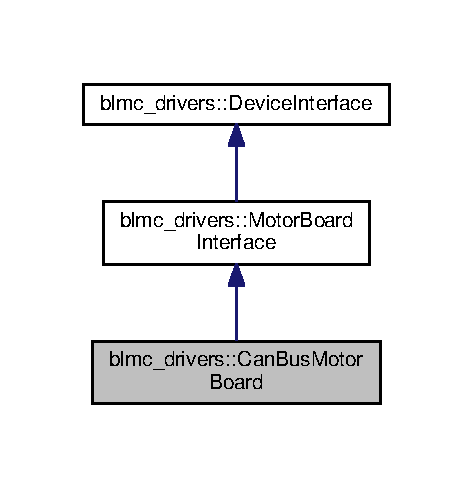
\includegraphics[width=227pt]{classblmc__drivers_1_1CanBusMotorBoard__inherit__graph}
\end{center}
\end{figure}


Collaboration diagram for blmc\+\_\+drivers\+:\+:Can\+Bus\+Motor\+Board\+:
\nopagebreak
\begin{figure}[H]
\begin{center}
\leavevmode
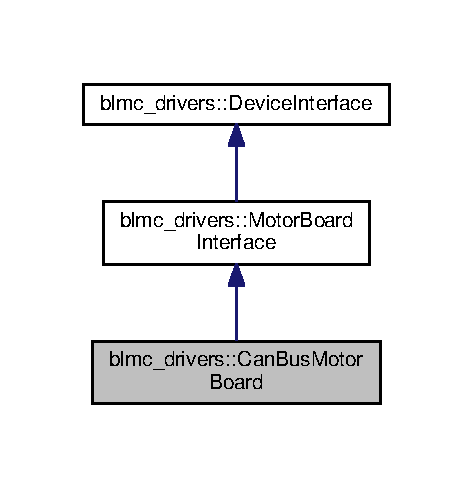
\includegraphics[width=227pt]{classblmc__drivers_1_1CanBusMotorBoard__coll__graph}
\end{center}
\end{figure}
\subsection*{Public Member Functions}
\begin{DoxyCompactItemize}
\item 
\hyperlink{classblmc__drivers_1_1CanBusMotorBoard_a43674811685fce4dbc3a9996e08454c9}{Can\+Bus\+Motor\+Board} (std\+::shared\+\_\+ptr$<$ \hyperlink{classblmc__drivers_1_1CanBusInterface}{Can\+Bus\+Interface} $>$ can\+\_\+bus, const size\+\_\+t \&history\+\_\+length=1000, const int \&control\+\_\+timeout\+\_\+ms=100)
\begin{DoxyCompactList}\small\item\em Construct a new \hyperlink{classblmc__drivers_1_1CanBusMotorBoard}{Can\+Bus\+Motor\+Board} object. \end{DoxyCompactList}\item 
\hyperlink{classblmc__drivers_1_1CanBusMotorBoard_a4099ee10765570b2bfb1f91a0670b11b}{$\sim$\+Can\+Bus\+Motor\+Board} ()\hypertarget{classblmc__drivers_1_1CanBusMotorBoard_a4099ee10765570b2bfb1f91a0670b11b}{}\label{classblmc__drivers_1_1CanBusMotorBoard_a4099ee10765570b2bfb1f91a0670b11b}

\begin{DoxyCompactList}\small\item\em Destroy the \hyperlink{classblmc__drivers_1_1CanBusMotorBoard}{Can\+Bus\+Motor\+Board} object. \end{DoxyCompactList}\item 
virtual \hyperlink{classblmc__drivers_1_1MotorBoardInterface_a6a733b7ed7a3a96f6b0712b6bb5307f8}{Ptr}$<$ const \hyperlink{classblmc__drivers_1_1MotorBoardInterface_a14e237254ba495a66091ea3a3a33fa75}{Scalar\+Timeseries} $>$ \hyperlink{classblmc__drivers_1_1CanBusMotorBoard_a38094207eed00f6b1d75cfe9b5b87046}{get\+\_\+measurement} (const int \&index) const 
\begin{DoxyCompactList}\small\item\em Getters. \end{DoxyCompactList}\item 
virtual \hyperlink{classblmc__drivers_1_1MotorBoardInterface_a6a733b7ed7a3a96f6b0712b6bb5307f8}{Ptr}$<$ const \hyperlink{classblmc__drivers_1_1MotorBoardInterface_ae3777e484dda60c4abe87f2b542ddfb8}{Status\+Timeseries} $>$ \hyperlink{classblmc__drivers_1_1CanBusMotorBoard_a04aef38d8490ed8ac0e12cb09ef313e4}{get\+\_\+status} () const 
\begin{DoxyCompactList}\small\item\em Get the status of the C\+AN card. \end{DoxyCompactList}\item 
virtual \hyperlink{classblmc__drivers_1_1MotorBoardInterface_a6a733b7ed7a3a96f6b0712b6bb5307f8}{Ptr}$<$ const \hyperlink{classblmc__drivers_1_1MotorBoardInterface_a14e237254ba495a66091ea3a3a33fa75}{Scalar\+Timeseries} $>$ \hyperlink{classblmc__drivers_1_1CanBusMotorBoard_a298403ab64585ed459eda57165057fef}{get\+\_\+control} (const int \&index) const 
\begin{DoxyCompactList}\small\item\em Get the controls to be sent. \end{DoxyCompactList}\item 
virtual \hyperlink{classblmc__drivers_1_1MotorBoardInterface_a6a733b7ed7a3a96f6b0712b6bb5307f8}{Ptr}$<$ const \hyperlink{classblmc__drivers_1_1MotorBoardInterface_ae2afe94a023d9f08a4c689e9b7660f15}{Command\+Timeseries} $>$ \hyperlink{classblmc__drivers_1_1CanBusMotorBoard_abc8f5d6a631dc01a236d623754362e7d}{get\+\_\+command} () const 
\begin{DoxyCompactList}\small\item\em Get the commands to be sent. \end{DoxyCompactList}\item 
virtual \hyperlink{classblmc__drivers_1_1MotorBoardInterface_a6a733b7ed7a3a96f6b0712b6bb5307f8}{Ptr}$<$ const \hyperlink{classblmc__drivers_1_1MotorBoardInterface_a14e237254ba495a66091ea3a3a33fa75}{Scalar\+Timeseries} $>$ \hyperlink{classblmc__drivers_1_1CanBusMotorBoard_a907629485fcf006e1e61b9739d3c94ec}{get\+\_\+sent\+\_\+control} (const int \&index) const 
\begin{DoxyCompactList}\small\item\em Get the already sent controls. \end{DoxyCompactList}\item 
virtual \hyperlink{classblmc__drivers_1_1MotorBoardInterface_a6a733b7ed7a3a96f6b0712b6bb5307f8}{Ptr}$<$ const \hyperlink{classblmc__drivers_1_1MotorBoardInterface_ae2afe94a023d9f08a4c689e9b7660f15}{Command\+Timeseries} $>$ \hyperlink{classblmc__drivers_1_1CanBusMotorBoard_a4e2920571e42aafa8045d1148f078a3a}{get\+\_\+sent\+\_\+command} () const 
\begin{DoxyCompactList}\small\item\em Get the already sent commands. \end{DoxyCompactList}\item 
virtual void \hyperlink{classblmc__drivers_1_1CanBusMotorBoard_a8dbd787fcfc25d68d5443e2f0bf21f64}{set\+\_\+control} (const double \&control, const int \&index)
\begin{DoxyCompactList}\small\item\em Setters. \end{DoxyCompactList}\item 
virtual void \hyperlink{classblmc__drivers_1_1CanBusMotorBoard_a4bb9c1f7f59507feed145111ccffc625}{set\+\_\+command} (const \hyperlink{classblmc__drivers_1_1MotorBoardCommand}{Motor\+Board\+Command} \&command)
\begin{DoxyCompactList}\small\item\em Set the commands, see \hyperlink{classblmc__drivers_1_1MotorBoardInterface_a86b4ff810ca652d6761090ceaff65621}{Motor\+Board\+Interface\+::set\+\_\+command}. \end{DoxyCompactList}\item 
virtual void \hyperlink{classblmc__drivers_1_1CanBusMotorBoard_a19ced11d06984528e6a2308c03ba83ac}{send\+\_\+if\+\_\+input\+\_\+changed} ()\hypertarget{classblmc__drivers_1_1CanBusMotorBoard_a19ced11d06984528e6a2308c03ba83ac}{}\label{classblmc__drivers_1_1CanBusMotorBoard_a19ced11d06984528e6a2308c03ba83ac}

\begin{DoxyCompactList}\small\item\em Send the actual command and controls. \end{DoxyCompactList}\item 
void \hyperlink{classblmc__drivers_1_1CanBusMotorBoard_a3c496f045d3ef68c02fe6dd5abbdc4eb}{wait\+\_\+until\+\_\+ready} ()\hypertarget{classblmc__drivers_1_1CanBusMotorBoard_a3c496f045d3ef68c02fe6dd5abbdc4eb}{}\label{classblmc__drivers_1_1CanBusMotorBoard_a3c496f045d3ef68c02fe6dd5abbdc4eb}

\begin{DoxyCompactList}\small\item\em returns only once board and motors are ready. \end{DoxyCompactList}\item 
bool {\bfseries is\+\_\+ready} ()\hypertarget{classblmc__drivers_1_1CanBusMotorBoard_aecd2ba0d3d1f40ffd38a0fd47b8da55d}{}\label{classblmc__drivers_1_1CanBusMotorBoard_aecd2ba0d3d1f40ffd38a0fd47b8da55d}

\item 
void \hyperlink{classblmc__drivers_1_1CanBusMotorBoard_a19ffd7d9ef9a441299164485e85ec6fd}{pause\+\_\+motors} ()
\item 
void \hyperlink{classblmc__drivers_1_1CanBusMotorBoard_a846382d2ad74d2087f5557ecd90937e3}{disable\+\_\+can\+\_\+recv\+\_\+timeout} ()\hypertarget{classblmc__drivers_1_1CanBusMotorBoard_a846382d2ad74d2087f5557ecd90937e3}{}\label{classblmc__drivers_1_1CanBusMotorBoard_a846382d2ad74d2087f5557ecd90937e3}

\begin{DoxyCompactList}\small\item\em Disable the can reciever timeout. \end{DoxyCompactList}\end{DoxyCompactItemize}
\subsection*{Private Types}
\begin{DoxyCompactItemize}
\item 
enum \hyperlink{classblmc__drivers_1_1CanBusMotorBoard_addbf32fe0b6fa57134546c1f6ec5eb80}{Canframe\+I\+Ds} \{ \\*
{\bfseries C\+O\+M\+M\+A\+N\+D\+\_\+\+ID} = 0x00, 
{\bfseries Iq\+Ref} = 0x05, 
{\bfseries S\+T\+A\+T\+U\+S\+M\+SG} = 0x10, 
{\bfseries Iq} = 0x20, 
\\*
{\bfseries P\+OS} = 0x30, 
{\bfseries S\+P\+E\+ED} = 0x40, 
{\bfseries A\+D\+C6} = 0x50, 
{\bfseries E\+N\+C\+\_\+\+I\+N\+D\+EX} = 0x60
 \}\hypertarget{classblmc__drivers_1_1CanBusMotorBoard_addbf32fe0b6fa57134546c1f6ec5eb80}{}\label{classblmc__drivers_1_1CanBusMotorBoard_addbf32fe0b6fa57134546c1f6ec5eb80}
\begin{DoxyCompactList}\small\item\em These are the frame I\+Ds that define the kind of data we acquiere from the C\+AN bus. \end{DoxyCompactList}
\end{DoxyCompactItemize}
\subsection*{Private Member Functions}
\begin{DoxyCompactItemize}
\item 
{\footnotesize template$<$typename T $>$ }\\int32\+\_\+t \hyperlink{classblmc__drivers_1_1CanBusMotorBoard_ae320518f2cf2c8af0e50220f11556b85}{bytes\+\_\+to\+\_\+int32} (T bytes)
\begin{DoxyCompactList}\small\item\em private methods ======================================================== \end{DoxyCompactList}\item 
float \hyperlink{classblmc__drivers_1_1CanBusMotorBoard_a05db7868ff7034289358cdb774b59720}{q24\+\_\+to\+\_\+float} (int32\+\_\+t qval)
\begin{DoxyCompactList}\small\item\em Convert from 24-\/bit normalized fixed-\/point to float. \end{DoxyCompactList}\item 
int32\+\_\+t \hyperlink{classblmc__drivers_1_1CanBusMotorBoard_ad6d91ccf867e9a3996492cce33270426}{float\+\_\+to\+\_\+q24} (float fval)
\begin{DoxyCompactList}\small\item\em Converts from float to 24-\/bit normalized fixed-\/point. \end{DoxyCompactList}\item 
{\footnotesize template$<$typename T $>$ }\\float \hyperlink{classblmc__drivers_1_1CanBusMotorBoard_ad2cee731d455d64d71014c9821219410}{qbytes\+\_\+to\+\_\+float} (T qbytes)
\begin{DoxyCompactList}\small\item\em Converts from qbytes to float. \end{DoxyCompactList}\item 
void \hyperlink{classblmc__drivers_1_1CanBusMotorBoard_a5ec842674fd543a8c834265433740387}{send\+\_\+newest\+\_\+controls} ()
\begin{DoxyCompactList}\small\item\em send the controls to the cards. \end{DoxyCompactList}\item 
void \hyperlink{classblmc__drivers_1_1CanBusMotorBoard_a9f74868318daf4a97a5266e4d8d6f556}{send\+\_\+newest\+\_\+command} ()\hypertarget{classblmc__drivers_1_1CanBusMotorBoard_a9f74868318daf4a97a5266e4d8d6f556}{}\label{classblmc__drivers_1_1CanBusMotorBoard_a9f74868318daf4a97a5266e4d8d6f556}

\begin{DoxyCompactList}\small\item\em send the latest commands to the cards. \end{DoxyCompactList}\item 
void \hyperlink{classblmc__drivers_1_1CanBusMotorBoard_a542f8df35ff34348976ed1d55797a15a}{loop} ()\hypertarget{classblmc__drivers_1_1CanBusMotorBoard_a542f8df35ff34348976ed1d55797a15a}{}\label{classblmc__drivers_1_1CanBusMotorBoard_a542f8df35ff34348976ed1d55797a15a}

\begin{DoxyCompactList}\small\item\em Is the loop that constently communicate with the network. \end{DoxyCompactList}\item 
void \hyperlink{classblmc__drivers_1_1CanBusMotorBoard_a43b773d56156d4855e6b3b7b7b00b350}{print\+\_\+status} ()\hypertarget{classblmc__drivers_1_1CanBusMotorBoard_a43b773d56156d4855e6b3b7b7b00b350}{}\label{classblmc__drivers_1_1CanBusMotorBoard_a43b773d56156d4855e6b3b7b7b00b350}

\begin{DoxyCompactList}\small\item\em Display details of this object. \end{DoxyCompactList}\end{DoxyCompactItemize}
\subsection*{Static Private Member Functions}
\begin{DoxyCompactItemize}
\item 
static T\+H\+R\+E\+A\+D\+\_\+\+F\+U\+N\+C\+T\+I\+O\+N\+\_\+\+R\+E\+T\+U\+R\+N\+\_\+\+T\+Y\+PE \hyperlink{classblmc__drivers_1_1CanBusMotorBoard_af6d242ea933e9ad23c37167ba848f017}{loop} (void $\ast$instance\+\_\+pointer)
\begin{DoxyCompactList}\small\item\em This is the helper function used for spawning the real time thread. \end{DoxyCompactList}\end{DoxyCompactItemize}
\subsection*{Private Attributes}
\begin{DoxyCompactItemize}
\item 
std\+::shared\+\_\+ptr$<$ \hyperlink{classblmc__drivers_1_1CanBusInterface}{Can\+Bus\+Interface} $>$ \hyperlink{classblmc__drivers_1_1CanBusMotorBoard_ab58dc93d9117503950fbe4d7a7c70914}{can\+\_\+bus\+\_\+}\hypertarget{classblmc__drivers_1_1CanBusMotorBoard_ab58dc93d9117503950fbe4d7a7c70914}{}\label{classblmc__drivers_1_1CanBusMotorBoard_ab58dc93d9117503950fbe4d7a7c70914}

\begin{DoxyCompactList}\small\item\em This is the pointer to the can bus to communicate with. \end{DoxyCompactList}\item 
\hyperlink{classblmc__drivers_1_1MotorBoardInterface_abeb474bef6d85dffcd5227e5ea965cc5}{Vector}$<$ \hyperlink{classblmc__drivers_1_1MotorBoardInterface_a6a733b7ed7a3a96f6b0712b6bb5307f8}{Ptr}$<$ \hyperlink{classblmc__drivers_1_1MotorBoardInterface_a14e237254ba495a66091ea3a3a33fa75}{Scalar\+Timeseries} $>$ $>$ \hyperlink{classblmc__drivers_1_1CanBusMotorBoard_abbba6ad698905e56101c516baa795b29}{measurement\+\_\+}
\begin{DoxyCompactList}\small\item\em Outputs. \end{DoxyCompactList}\item 
\hyperlink{classblmc__drivers_1_1MotorBoardInterface_a6a733b7ed7a3a96f6b0712b6bb5307f8}{Ptr}$<$ \hyperlink{classblmc__drivers_1_1MotorBoardInterface_ae3777e484dda60c4abe87f2b542ddfb8}{Status\+Timeseries} $>$ \hyperlink{classblmc__drivers_1_1CanBusMotorBoard_a5725ff23bb4f8407c5608cabfa49c692}{status\+\_\+}\hypertarget{classblmc__drivers_1_1CanBusMotorBoard_a5725ff23bb4f8407c5608cabfa49c692}{}\label{classblmc__drivers_1_1CanBusMotorBoard_a5725ff23bb4f8407c5608cabfa49c692}

\begin{DoxyCompactList}\small\item\em This is the status history of the C\+AN board. \end{DoxyCompactList}\item 
\hyperlink{classblmc__drivers_1_1MotorBoardInterface_abeb474bef6d85dffcd5227e5ea965cc5}{Vector}$<$ \hyperlink{classblmc__drivers_1_1MotorBoardInterface_a6a733b7ed7a3a96f6b0712b6bb5307f8}{Ptr}$<$ \hyperlink{classblmc__drivers_1_1MotorBoardInterface_a14e237254ba495a66091ea3a3a33fa75}{Scalar\+Timeseries} $>$ $>$ \hyperlink{classblmc__drivers_1_1CanBusMotorBoard_a65cfba005239247df1ea26795ff14a3f}{control\+\_\+}
\begin{DoxyCompactList}\small\item\em Inputs. \end{DoxyCompactList}\item 
\hyperlink{classblmc__drivers_1_1MotorBoardInterface_a6a733b7ed7a3a96f6b0712b6bb5307f8}{Ptr}$<$ \hyperlink{classblmc__drivers_1_1MotorBoardInterface_ae2afe94a023d9f08a4c689e9b7660f15}{Command\+Timeseries} $>$ \hyperlink{classblmc__drivers_1_1CanBusMotorBoard_a720c6300bf07245a739713a209799c02}{command\+\_\+}\hypertarget{classblmc__drivers_1_1CanBusMotorBoard_a720c6300bf07245a739713a209799c02}{}\label{classblmc__drivers_1_1CanBusMotorBoard_a720c6300bf07245a739713a209799c02}

\begin{DoxyCompactList}\small\item\em This is the buffer of the commands to be sent to the card. \end{DoxyCompactList}\item 
\hyperlink{classblmc__drivers_1_1MotorBoardInterface_abeb474bef6d85dffcd5227e5ea965cc5}{Vector}$<$ \hyperlink{classblmc__drivers_1_1MotorBoardInterface_a6a733b7ed7a3a96f6b0712b6bb5307f8}{Ptr}$<$ \hyperlink{classblmc__drivers_1_1MotorBoardInterface_a14e237254ba495a66091ea3a3a33fa75}{Scalar\+Timeseries} $>$ $>$ \hyperlink{classblmc__drivers_1_1CanBusMotorBoard_ab5296d55684d48b538844c3b96df6594}{sent\+\_\+control\+\_\+}
\begin{DoxyCompactList}\small\item\em Log. \end{DoxyCompactList}\item 
\hyperlink{classblmc__drivers_1_1MotorBoardInterface_a6a733b7ed7a3a96f6b0712b6bb5307f8}{Ptr}$<$ \hyperlink{classblmc__drivers_1_1MotorBoardInterface_ae2afe94a023d9f08a4c689e9b7660f15}{Command\+Timeseries} $>$ \hyperlink{classblmc__drivers_1_1CanBusMotorBoard_a27712df32104357ac31b97179f1e9211}{sent\+\_\+command\+\_\+}\hypertarget{classblmc__drivers_1_1CanBusMotorBoard_a27712df32104357ac31b97179f1e9211}{}\label{classblmc__drivers_1_1CanBusMotorBoard_a27712df32104357ac31b97179f1e9211}

\begin{DoxyCompactList}\small\item\em This is the history of the already sent commands. \end{DoxyCompactList}\item 
bool \hyperlink{classblmc__drivers_1_1CanBusMotorBoard_ae25808cc09839c2574d134a36b5b4d5d}{is\+\_\+loop\+\_\+active\+\_\+}
\begin{DoxyCompactList}\small\item\em Loop management. \end{DoxyCompactList}\item 
bool \hyperlink{classblmc__drivers_1_1CanBusMotorBoard_abdca3f76908ca197c4f12af814313a56}{motors\+\_\+are\+\_\+paused\+\_\+}\hypertarget{classblmc__drivers_1_1CanBusMotorBoard_abdca3f76908ca197c4f12af814313a56}{}\label{classblmc__drivers_1_1CanBusMotorBoard_abdca3f76908ca197c4f12af814313a56}

\begin{DoxyCompactList}\small\item\em Are motor in idle mode = 0 torques?  update this documentation with the actual behavior. \end{DoxyCompactList}\item 
int \hyperlink{classblmc__drivers_1_1CanBusMotorBoard_a4f9605b0a147ecd1dde41a0fb7b45d47}{control\+\_\+timeout\+\_\+ms\+\_\+}\hypertarget{classblmc__drivers_1_1CanBusMotorBoard_a4f9605b0a147ecd1dde41a0fb7b45d47}{}\label{classblmc__drivers_1_1CanBusMotorBoard_a4f9605b0a147ecd1dde41a0fb7b45d47}

\begin{DoxyCompactList}\small\item\em If no control is sent for more than control\+\_\+timeout\+\_\+ms\+\_\+ the board will shut down. \end{DoxyCompactList}\item 
real\+\_\+time\+\_\+tools\+::\+Real\+Time\+Thread \hyperlink{classblmc__drivers_1_1CanBusMotorBoard_a040b0b2f6c2691a54d82404f7a1badd6}{rt\+\_\+thread\+\_\+}\hypertarget{classblmc__drivers_1_1CanBusMotorBoard_a040b0b2f6c2691a54d82404f7a1badd6}{}\label{classblmc__drivers_1_1CanBusMotorBoard_a040b0b2f6c2691a54d82404f7a1badd6}

\begin{DoxyCompactList}\small\item\em This is the thread object that allow to spwan a real-\/time thread or not dependening on the current OS. \end{DoxyCompactList}\end{DoxyCompactItemize}
\subsection*{Additional Inherited Members}


\subsection{Detailed Description}
This class \hyperlink{classblmc__drivers_1_1CanBusMotorBoard}{Can\+Bus\+Motor\+Board} implements a \hyperlink{classblmc__drivers_1_1MotorBoardInterface}{Motor\+Board\+Interface} specific to C\+AN networks. 

\subsection{Constructor \& Destructor Documentation}
\index{blmc\+\_\+drivers\+::\+Can\+Bus\+Motor\+Board@{blmc\+\_\+drivers\+::\+Can\+Bus\+Motor\+Board}!Can\+Bus\+Motor\+Board@{Can\+Bus\+Motor\+Board}}
\index{Can\+Bus\+Motor\+Board@{Can\+Bus\+Motor\+Board}!blmc\+\_\+drivers\+::\+Can\+Bus\+Motor\+Board@{blmc\+\_\+drivers\+::\+Can\+Bus\+Motor\+Board}}
\subsubsection[{\texorpdfstring{Can\+Bus\+Motor\+Board(std\+::shared\+\_\+ptr$<$ Can\+Bus\+Interface $>$ can\+\_\+bus, const size\+\_\+t \&history\+\_\+length=1000, const int \&control\+\_\+timeout\+\_\+ms=100)}{CanBusMotorBoard(std::shared_ptr< CanBusInterface > can_bus, const size_t &history_length=1000, const int &control_timeout_ms=100)}}]{\setlength{\rightskip}{0pt plus 5cm}blmc\+\_\+drivers\+::\+Can\+Bus\+Motor\+Board\+::\+Can\+Bus\+Motor\+Board (
\begin{DoxyParamCaption}
\item[{std\+::shared\+\_\+ptr$<$ {\bf Can\+Bus\+Interface} $>$}]{can\+\_\+bus, }
\item[{const size\+\_\+t \&}]{history\+\_\+length = {\ttfamily 1000}, }
\item[{const int \&}]{control\+\_\+timeout\+\_\+ms = {\ttfamily 100}}
\end{DoxyParamCaption}
)}\hypertarget{classblmc__drivers_1_1CanBusMotorBoard_a43674811685fce4dbc3a9996e08454c9}{}\label{classblmc__drivers_1_1CanBusMotorBoard_a43674811685fce4dbc3a9996e08454c9}


Construct a new \hyperlink{classblmc__drivers_1_1CanBusMotorBoard}{Can\+Bus\+Motor\+Board} object. 


\begin{DoxyParams}{Parameters}
{\em can\+\_\+bus} & \\
\hline
{\em history\+\_\+length} & \\
\hline
\end{DoxyParams}


\subsection{Member Function Documentation}
\index{blmc\+\_\+drivers\+::\+Can\+Bus\+Motor\+Board@{blmc\+\_\+drivers\+::\+Can\+Bus\+Motor\+Board}!bytes\+\_\+to\+\_\+int32@{bytes\+\_\+to\+\_\+int32}}
\index{bytes\+\_\+to\+\_\+int32@{bytes\+\_\+to\+\_\+int32}!blmc\+\_\+drivers\+::\+Can\+Bus\+Motor\+Board@{blmc\+\_\+drivers\+::\+Can\+Bus\+Motor\+Board}}
\subsubsection[{\texorpdfstring{bytes\+\_\+to\+\_\+int32(\+T bytes)}{bytes_to_int32(T bytes)}}]{\setlength{\rightskip}{0pt plus 5cm}template$<$typename T $>$ int32\+\_\+t blmc\+\_\+drivers\+::\+Can\+Bus\+Motor\+Board\+::bytes\+\_\+to\+\_\+int32 (
\begin{DoxyParamCaption}
\item[{T}]{bytes}
\end{DoxyParamCaption}
)\hspace{0.3cm}{\ttfamily [inline]}, {\ttfamily [private]}}\hypertarget{classblmc__drivers_1_1CanBusMotorBoard_ae320518f2cf2c8af0e50220f11556b85}{}\label{classblmc__drivers_1_1CanBusMotorBoard_ae320518f2cf2c8af0e50220f11556b85}


private methods ======================================================== 

Useful converters Converts from bytes to int32.


\begin{DoxyTemplParams}{Template Parameters}
{\em T} & this is the type of the bytes convert. \\
\hline
\end{DoxyTemplParams}

\begin{DoxyParams}{Parameters}
{\em bytes} & The bytes value \\
\hline
\end{DoxyParams}
\begin{DoxyReturn}{Returns}
int32\+\_\+t the output integer in int32. 
\end{DoxyReturn}
\index{blmc\+\_\+drivers\+::\+Can\+Bus\+Motor\+Board@{blmc\+\_\+drivers\+::\+Can\+Bus\+Motor\+Board}!float\+\_\+to\+\_\+q24@{float\+\_\+to\+\_\+q24}}
\index{float\+\_\+to\+\_\+q24@{float\+\_\+to\+\_\+q24}!blmc\+\_\+drivers\+::\+Can\+Bus\+Motor\+Board@{blmc\+\_\+drivers\+::\+Can\+Bus\+Motor\+Board}}
\subsubsection[{\texorpdfstring{float\+\_\+to\+\_\+q24(float fval)}{float_to_q24(float fval)}}]{\setlength{\rightskip}{0pt plus 5cm}int32\+\_\+t blmc\+\_\+drivers\+::\+Can\+Bus\+Motor\+Board\+::float\+\_\+to\+\_\+q24 (
\begin{DoxyParamCaption}
\item[{float}]{fval}
\end{DoxyParamCaption}
)\hspace{0.3cm}{\ttfamily [inline]}, {\ttfamily [private]}}\hypertarget{classblmc__drivers_1_1CanBusMotorBoard_ad6d91ccf867e9a3996492cce33270426}{}\label{classblmc__drivers_1_1CanBusMotorBoard_ad6d91ccf867e9a3996492cce33270426}


Converts from float to 24-\/bit normalized fixed-\/point. 


\begin{DoxyParams}{Parameters}
{\em fval} & \\
\hline
\end{DoxyParams}
\begin{DoxyReturn}{Returns}
int32\+\_\+t 
\end{DoxyReturn}
\index{blmc\+\_\+drivers\+::\+Can\+Bus\+Motor\+Board@{blmc\+\_\+drivers\+::\+Can\+Bus\+Motor\+Board}!get\+\_\+command@{get\+\_\+command}}
\index{get\+\_\+command@{get\+\_\+command}!blmc\+\_\+drivers\+::\+Can\+Bus\+Motor\+Board@{blmc\+\_\+drivers\+::\+Can\+Bus\+Motor\+Board}}
\subsubsection[{\texorpdfstring{get\+\_\+command() const }{get_command() const }}]{\setlength{\rightskip}{0pt plus 5cm}virtual {\bf Ptr}$<$const {\bf Command\+Timeseries}$>$ blmc\+\_\+drivers\+::\+Can\+Bus\+Motor\+Board\+::get\+\_\+command (
\begin{DoxyParamCaption}
{}
\end{DoxyParamCaption}
) const\hspace{0.3cm}{\ttfamily [inline]}, {\ttfamily [virtual]}}\hypertarget{classblmc__drivers_1_1CanBusMotorBoard_abc8f5d6a631dc01a236d623754362e7d}{}\label{classblmc__drivers_1_1CanBusMotorBoard_abc8f5d6a631dc01a236d623754362e7d}


Get the commands to be sent. 

\begin{DoxyReturn}{Returns}
Ptr$<$const Command\+Timeseries$>$ is the list of the command to be sent. 
\end{DoxyReturn}


Implements \hyperlink{classblmc__drivers_1_1MotorBoardInterface_a4913308c1eacc98475aeb8647447c997}{blmc\+\_\+drivers\+::\+Motor\+Board\+Interface}.

\index{blmc\+\_\+drivers\+::\+Can\+Bus\+Motor\+Board@{blmc\+\_\+drivers\+::\+Can\+Bus\+Motor\+Board}!get\+\_\+control@{get\+\_\+control}}
\index{get\+\_\+control@{get\+\_\+control}!blmc\+\_\+drivers\+::\+Can\+Bus\+Motor\+Board@{blmc\+\_\+drivers\+::\+Can\+Bus\+Motor\+Board}}
\subsubsection[{\texorpdfstring{get\+\_\+control(const int \&index) const }{get_control(const int &index) const }}]{\setlength{\rightskip}{0pt plus 5cm}virtual {\bf Ptr}$<$const {\bf Scalar\+Timeseries}$>$ blmc\+\_\+drivers\+::\+Can\+Bus\+Motor\+Board\+::get\+\_\+control (
\begin{DoxyParamCaption}
\item[{const int \&}]{index}
\end{DoxyParamCaption}
) const\hspace{0.3cm}{\ttfamily [inline]}, {\ttfamily [virtual]}}\hypertarget{classblmc__drivers_1_1CanBusMotorBoard_a298403ab64585ed459eda57165057fef}{}\label{classblmc__drivers_1_1CanBusMotorBoard_a298403ab64585ed459eda57165057fef}


Get the controls to be sent. 


\begin{DoxyParams}{Parameters}
{\em index} & the kind of control we are interested in. \\
\hline
\end{DoxyParams}
\begin{DoxyReturn}{Returns}
Ptr$<$const Scalar\+Timeseries$>$ is the list of the control to be sent. 
\end{DoxyReturn}


Implements \hyperlink{classblmc__drivers_1_1MotorBoardInterface_aa5eeed12c851993f2e2c93f5479df9de}{blmc\+\_\+drivers\+::\+Motor\+Board\+Interface}.

\index{blmc\+\_\+drivers\+::\+Can\+Bus\+Motor\+Board@{blmc\+\_\+drivers\+::\+Can\+Bus\+Motor\+Board}!get\+\_\+measurement@{get\+\_\+measurement}}
\index{get\+\_\+measurement@{get\+\_\+measurement}!blmc\+\_\+drivers\+::\+Can\+Bus\+Motor\+Board@{blmc\+\_\+drivers\+::\+Can\+Bus\+Motor\+Board}}
\subsubsection[{\texorpdfstring{get\+\_\+measurement(const int \&index) const }{get_measurement(const int &index) const }}]{\setlength{\rightskip}{0pt plus 5cm}virtual {\bf Ptr}$<$const {\bf Scalar\+Timeseries}$>$ blmc\+\_\+drivers\+::\+Can\+Bus\+Motor\+Board\+::get\+\_\+measurement (
\begin{DoxyParamCaption}
\item[{const int \&}]{index}
\end{DoxyParamCaption}
) const\hspace{0.3cm}{\ttfamily [inline]}, {\ttfamily [virtual]}}\hypertarget{classblmc__drivers_1_1CanBusMotorBoard_a38094207eed00f6b1d75cfe9b5b87046}{}\label{classblmc__drivers_1_1CanBusMotorBoard_a38094207eed00f6b1d75cfe9b5b87046}


Getters. 

Get the measurement data.


\begin{DoxyParams}{Parameters}
{\em index} & is the kind of measurement we are insterested in. \\
\hline
\end{DoxyParams}
\begin{DoxyReturn}{Returns}
Ptr$<$const Scalar\+Timeseries$>$ is the list of the last measurements acquiered from the C\+AN card. 
\end{DoxyReturn}


Implements \hyperlink{classblmc__drivers_1_1MotorBoardInterface_a34828a0375a3bd1fede4deb4fc74c04d}{blmc\+\_\+drivers\+::\+Motor\+Board\+Interface}.

\index{blmc\+\_\+drivers\+::\+Can\+Bus\+Motor\+Board@{blmc\+\_\+drivers\+::\+Can\+Bus\+Motor\+Board}!get\+\_\+sent\+\_\+command@{get\+\_\+sent\+\_\+command}}
\index{get\+\_\+sent\+\_\+command@{get\+\_\+sent\+\_\+command}!blmc\+\_\+drivers\+::\+Can\+Bus\+Motor\+Board@{blmc\+\_\+drivers\+::\+Can\+Bus\+Motor\+Board}}
\subsubsection[{\texorpdfstring{get\+\_\+sent\+\_\+command() const }{get_sent_command() const }}]{\setlength{\rightskip}{0pt plus 5cm}virtual {\bf Ptr}$<$const {\bf Command\+Timeseries}$>$ blmc\+\_\+drivers\+::\+Can\+Bus\+Motor\+Board\+::get\+\_\+sent\+\_\+command (
\begin{DoxyParamCaption}
{}
\end{DoxyParamCaption}
) const\hspace{0.3cm}{\ttfamily [inline]}, {\ttfamily [virtual]}}\hypertarget{classblmc__drivers_1_1CanBusMotorBoard_a4e2920571e42aafa8045d1148f078a3a}{}\label{classblmc__drivers_1_1CanBusMotorBoard_a4e2920571e42aafa8045d1148f078a3a}


Get the already sent commands. 

\begin{DoxyReturn}{Returns}
Ptr$<$const Command\+Timeseries$>$ is the list of the sent cotnrols. 
\end{DoxyReturn}


Implements \hyperlink{classblmc__drivers_1_1MotorBoardInterface_afd3de58f7a900347154b8d323f1c1d94}{blmc\+\_\+drivers\+::\+Motor\+Board\+Interface}.

\index{blmc\+\_\+drivers\+::\+Can\+Bus\+Motor\+Board@{blmc\+\_\+drivers\+::\+Can\+Bus\+Motor\+Board}!get\+\_\+sent\+\_\+control@{get\+\_\+sent\+\_\+control}}
\index{get\+\_\+sent\+\_\+control@{get\+\_\+sent\+\_\+control}!blmc\+\_\+drivers\+::\+Can\+Bus\+Motor\+Board@{blmc\+\_\+drivers\+::\+Can\+Bus\+Motor\+Board}}
\subsubsection[{\texorpdfstring{get\+\_\+sent\+\_\+control(const int \&index) const }{get_sent_control(const int &index) const }}]{\setlength{\rightskip}{0pt plus 5cm}virtual {\bf Ptr}$<$const {\bf Scalar\+Timeseries}$>$ blmc\+\_\+drivers\+::\+Can\+Bus\+Motor\+Board\+::get\+\_\+sent\+\_\+control (
\begin{DoxyParamCaption}
\item[{const int \&}]{index}
\end{DoxyParamCaption}
) const\hspace{0.3cm}{\ttfamily [inline]}, {\ttfamily [virtual]}}\hypertarget{classblmc__drivers_1_1CanBusMotorBoard_a907629485fcf006e1e61b9739d3c94ec}{}\label{classblmc__drivers_1_1CanBusMotorBoard_a907629485fcf006e1e61b9739d3c94ec}


Get the already sent controls. 


\begin{DoxyParams}{Parameters}
{\em index} & the kind of control we are interested in. \\
\hline
\end{DoxyParams}
\begin{DoxyReturn}{Returns}
Ptr$<$const Scalar\+Timeseries$>$ is the list of the sent cotnrols. 
\end{DoxyReturn}


Implements \hyperlink{classblmc__drivers_1_1MotorBoardInterface_a8dc6222e915fc96d89b13cbb0fcb0cda}{blmc\+\_\+drivers\+::\+Motor\+Board\+Interface}.

\index{blmc\+\_\+drivers\+::\+Can\+Bus\+Motor\+Board@{blmc\+\_\+drivers\+::\+Can\+Bus\+Motor\+Board}!get\+\_\+status@{get\+\_\+status}}
\index{get\+\_\+status@{get\+\_\+status}!blmc\+\_\+drivers\+::\+Can\+Bus\+Motor\+Board@{blmc\+\_\+drivers\+::\+Can\+Bus\+Motor\+Board}}
\subsubsection[{\texorpdfstring{get\+\_\+status() const }{get_status() const }}]{\setlength{\rightskip}{0pt plus 5cm}virtual {\bf Ptr}$<$const {\bf Status\+Timeseries}$>$ blmc\+\_\+drivers\+::\+Can\+Bus\+Motor\+Board\+::get\+\_\+status (
\begin{DoxyParamCaption}
{}
\end{DoxyParamCaption}
) const\hspace{0.3cm}{\ttfamily [inline]}, {\ttfamily [virtual]}}\hypertarget{classblmc__drivers_1_1CanBusMotorBoard_a04aef38d8490ed8ac0e12cb09ef313e4}{}\label{classblmc__drivers_1_1CanBusMotorBoard_a04aef38d8490ed8ac0e12cb09ef313e4}


Get the status of the C\+AN card. 

\begin{DoxyReturn}{Returns}
Ptr$<$const Status\+Timeseries$>$ is the list of last acquiered status. 
\end{DoxyReturn}


Implements \hyperlink{classblmc__drivers_1_1MotorBoardInterface_a13b1ffa7d10c1c753d76eaf5368714e3}{blmc\+\_\+drivers\+::\+Motor\+Board\+Interface}.

\index{blmc\+\_\+drivers\+::\+Can\+Bus\+Motor\+Board@{blmc\+\_\+drivers\+::\+Can\+Bus\+Motor\+Board}!loop@{loop}}
\index{loop@{loop}!blmc\+\_\+drivers\+::\+Can\+Bus\+Motor\+Board@{blmc\+\_\+drivers\+::\+Can\+Bus\+Motor\+Board}}
\subsubsection[{\texorpdfstring{loop(void $\ast$instance\+\_\+pointer)}{loop(void *instance_pointer)}}]{\setlength{\rightskip}{0pt plus 5cm}static T\+H\+R\+E\+A\+D\+\_\+\+F\+U\+N\+C\+T\+I\+O\+N\+\_\+\+R\+E\+T\+U\+R\+N\+\_\+\+T\+Y\+PE blmc\+\_\+drivers\+::\+Can\+Bus\+Motor\+Board\+::loop (
\begin{DoxyParamCaption}
\item[{void $\ast$}]{instance\+\_\+pointer}
\end{DoxyParamCaption}
)\hspace{0.3cm}{\ttfamily [inline]}, {\ttfamily [static]}, {\ttfamily [private]}}\hypertarget{classblmc__drivers_1_1CanBusMotorBoard_af6d242ea933e9ad23c37167ba848f017}{}\label{classblmc__drivers_1_1CanBusMotorBoard_af6d242ea933e9ad23c37167ba848f017}


This is the helper function used for spawning the real time thread. 


\begin{DoxyParams}{Parameters}
{\em instance\+\_\+pointer} & is the current object in this case. \\
\hline
\end{DoxyParams}
\begin{DoxyReturn}{Returns}
T\+H\+R\+E\+A\+D\+\_\+\+F\+U\+N\+C\+T\+I\+O\+N\+\_\+\+R\+E\+T\+U\+R\+N\+\_\+\+T\+Y\+PE depends on the current OS. 
\end{DoxyReturn}
\index{blmc\+\_\+drivers\+::\+Can\+Bus\+Motor\+Board@{blmc\+\_\+drivers\+::\+Can\+Bus\+Motor\+Board}!pause\+\_\+motors@{pause\+\_\+motors}}
\index{pause\+\_\+motors@{pause\+\_\+motors}!blmc\+\_\+drivers\+::\+Can\+Bus\+Motor\+Board@{blmc\+\_\+drivers\+::\+Can\+Bus\+Motor\+Board}}
\subsubsection[{\texorpdfstring{pause\+\_\+motors()}{pause_motors()}}]{\setlength{\rightskip}{0pt plus 5cm}void blmc\+\_\+drivers\+::\+Can\+Bus\+Motor\+Board\+::pause\+\_\+motors (
\begin{DoxyParamCaption}
{}
\end{DoxyParamCaption}
)}\hypertarget{classblmc__drivers_1_1CanBusMotorBoard_a19ffd7d9ef9a441299164485e85ec6fd}{}\label{classblmc__drivers_1_1CanBusMotorBoard_a19ffd7d9ef9a441299164485e85ec6fd}
\begin{DoxyRefDesc}{Todo}
\item[\hyperlink{todo__todo000003}{Todo}]\+: this function should go away, and we should add somewhere a warning in case there is a timeout \end{DoxyRefDesc}
\index{blmc\+\_\+drivers\+::\+Can\+Bus\+Motor\+Board@{blmc\+\_\+drivers\+::\+Can\+Bus\+Motor\+Board}!q24\+\_\+to\+\_\+float@{q24\+\_\+to\+\_\+float}}
\index{q24\+\_\+to\+\_\+float@{q24\+\_\+to\+\_\+float}!blmc\+\_\+drivers\+::\+Can\+Bus\+Motor\+Board@{blmc\+\_\+drivers\+::\+Can\+Bus\+Motor\+Board}}
\subsubsection[{\texorpdfstring{q24\+\_\+to\+\_\+float(int32\+\_\+t qval)}{q24_to_float(int32_t qval)}}]{\setlength{\rightskip}{0pt plus 5cm}float blmc\+\_\+drivers\+::\+Can\+Bus\+Motor\+Board\+::q24\+\_\+to\+\_\+float (
\begin{DoxyParamCaption}
\item[{int32\+\_\+t}]{qval}
\end{DoxyParamCaption}
)\hspace{0.3cm}{\ttfamily [inline]}, {\ttfamily [private]}}\hypertarget{classblmc__drivers_1_1CanBusMotorBoard_a05db7868ff7034289358cdb774b59720}{}\label{classblmc__drivers_1_1CanBusMotorBoard_a05db7868ff7034289358cdb774b59720}


Convert from 24-\/bit normalized fixed-\/point to float. 


\begin{DoxyParams}{Parameters}
{\em qval} & is the floating base point. \\
\hline
\end{DoxyParams}
\begin{DoxyReturn}{Returns}
float is the converted value 
\end{DoxyReturn}
\index{blmc\+\_\+drivers\+::\+Can\+Bus\+Motor\+Board@{blmc\+\_\+drivers\+::\+Can\+Bus\+Motor\+Board}!qbytes\+\_\+to\+\_\+float@{qbytes\+\_\+to\+\_\+float}}
\index{qbytes\+\_\+to\+\_\+float@{qbytes\+\_\+to\+\_\+float}!blmc\+\_\+drivers\+::\+Can\+Bus\+Motor\+Board@{blmc\+\_\+drivers\+::\+Can\+Bus\+Motor\+Board}}
\subsubsection[{\texorpdfstring{qbytes\+\_\+to\+\_\+float(\+T qbytes)}{qbytes_to_float(T qbytes)}}]{\setlength{\rightskip}{0pt plus 5cm}template$<$typename T $>$ float blmc\+\_\+drivers\+::\+Can\+Bus\+Motor\+Board\+::qbytes\+\_\+to\+\_\+float (
\begin{DoxyParamCaption}
\item[{T}]{qbytes}
\end{DoxyParamCaption}
)\hspace{0.3cm}{\ttfamily [inline]}, {\ttfamily [private]}}\hypertarget{classblmc__drivers_1_1CanBusMotorBoard_ad2cee731d455d64d71014c9821219410}{}\label{classblmc__drivers_1_1CanBusMotorBoard_ad2cee731d455d64d71014c9821219410}


Converts from qbytes to float. 


\begin{DoxyTemplParams}{Template Parameters}
{\em T} & the type of byte to manage \\
\hline
\end{DoxyTemplParams}

\begin{DoxyParams}{Parameters}
{\em qbytes} & the input value in bytes \\
\hline
\end{DoxyParams}
\begin{DoxyReturn}{Returns}
float the output value. 
\end{DoxyReturn}
\index{blmc\+\_\+drivers\+::\+Can\+Bus\+Motor\+Board@{blmc\+\_\+drivers\+::\+Can\+Bus\+Motor\+Board}!send\+\_\+newest\+\_\+controls@{send\+\_\+newest\+\_\+controls}}
\index{send\+\_\+newest\+\_\+controls@{send\+\_\+newest\+\_\+controls}!blmc\+\_\+drivers\+::\+Can\+Bus\+Motor\+Board@{blmc\+\_\+drivers\+::\+Can\+Bus\+Motor\+Board}}
\subsubsection[{\texorpdfstring{send\+\_\+newest\+\_\+controls()}{send_newest_controls()}}]{\setlength{\rightskip}{0pt plus 5cm}void blmc\+\_\+drivers\+::\+Can\+Bus\+Motor\+Board\+::send\+\_\+newest\+\_\+controls (
\begin{DoxyParamCaption}
{}
\end{DoxyParamCaption}
)\hspace{0.3cm}{\ttfamily [private]}}\hypertarget{classblmc__drivers_1_1CanBusMotorBoard_a5ec842674fd543a8c834265433740387}{}\label{classblmc__drivers_1_1CanBusMotorBoard_a5ec842674fd543a8c834265433740387}


send the controls to the cards. 


\begin{DoxyParams}{Parameters}
{\em controls} & are the controls to be sent. \\
\hline
\end{DoxyParams}
\index{blmc\+\_\+drivers\+::\+Can\+Bus\+Motor\+Board@{blmc\+\_\+drivers\+::\+Can\+Bus\+Motor\+Board}!set\+\_\+command@{set\+\_\+command}}
\index{set\+\_\+command@{set\+\_\+command}!blmc\+\_\+drivers\+::\+Can\+Bus\+Motor\+Board@{blmc\+\_\+drivers\+::\+Can\+Bus\+Motor\+Board}}
\subsubsection[{\texorpdfstring{set\+\_\+command(const Motor\+Board\+Command \&command)}{set_command(const MotorBoardCommand &command)}}]{\setlength{\rightskip}{0pt plus 5cm}virtual void blmc\+\_\+drivers\+::\+Can\+Bus\+Motor\+Board\+::set\+\_\+command (
\begin{DoxyParamCaption}
\item[{const {\bf Motor\+Board\+Command} \&}]{command}
\end{DoxyParamCaption}
)\hspace{0.3cm}{\ttfamily [inline]}, {\ttfamily [virtual]}}\hypertarget{classblmc__drivers_1_1CanBusMotorBoard_a4bb9c1f7f59507feed145111ccffc625}{}\label{classblmc__drivers_1_1CanBusMotorBoard_a4bb9c1f7f59507feed145111ccffc625}


Set the commands, see \hyperlink{classblmc__drivers_1_1MotorBoardInterface_a86b4ff810ca652d6761090ceaff65621}{Motor\+Board\+Interface\+::set\+\_\+command}. 


\begin{DoxyParams}{Parameters}
{\em command} & \\
\hline
\end{DoxyParams}


Implements \hyperlink{classblmc__drivers_1_1MotorBoardInterface_a86b4ff810ca652d6761090ceaff65621}{blmc\+\_\+drivers\+::\+Motor\+Board\+Interface}.

\index{blmc\+\_\+drivers\+::\+Can\+Bus\+Motor\+Board@{blmc\+\_\+drivers\+::\+Can\+Bus\+Motor\+Board}!set\+\_\+control@{set\+\_\+control}}
\index{set\+\_\+control@{set\+\_\+control}!blmc\+\_\+drivers\+::\+Can\+Bus\+Motor\+Board@{blmc\+\_\+drivers\+::\+Can\+Bus\+Motor\+Board}}
\subsubsection[{\texorpdfstring{set\+\_\+control(const double \&control, const int \&index)}{set_control(const double &control, const int &index)}}]{\setlength{\rightskip}{0pt plus 5cm}virtual void blmc\+\_\+drivers\+::\+Can\+Bus\+Motor\+Board\+::set\+\_\+control (
\begin{DoxyParamCaption}
\item[{const double \&}]{control, }
\item[{const int \&}]{index}
\end{DoxyParamCaption}
)\hspace{0.3cm}{\ttfamily [inline]}, {\ttfamily [virtual]}}\hypertarget{classblmc__drivers_1_1CanBusMotorBoard_a8dbd787fcfc25d68d5443e2f0bf21f64}{}\label{classblmc__drivers_1_1CanBusMotorBoard_a8dbd787fcfc25d68d5443e2f0bf21f64}


Setters. 

Set the controls, see \hyperlink{classblmc__drivers_1_1MotorBoardInterface_a3ace57ba3e09b9b3120d09303ff39a61}{Motor\+Board\+Interface\+::set\+\_\+control}


\begin{DoxyParams}{Parameters}
{\em control} & \\
\hline
{\em index} & \\
\hline
\end{DoxyParams}


Implements \hyperlink{classblmc__drivers_1_1MotorBoardInterface_a3ace57ba3e09b9b3120d09303ff39a61}{blmc\+\_\+drivers\+::\+Motor\+Board\+Interface}.



\subsection{Member Data Documentation}
\index{blmc\+\_\+drivers\+::\+Can\+Bus\+Motor\+Board@{blmc\+\_\+drivers\+::\+Can\+Bus\+Motor\+Board}!control\+\_\+@{control\+\_\+}}
\index{control\+\_\+@{control\+\_\+}!blmc\+\_\+drivers\+::\+Can\+Bus\+Motor\+Board@{blmc\+\_\+drivers\+::\+Can\+Bus\+Motor\+Board}}
\subsubsection[{\texorpdfstring{control\+\_\+}{control_}}]{\setlength{\rightskip}{0pt plus 5cm}{\bf Vector}$<${\bf Ptr}$<${\bf Scalar\+Timeseries}$>$ $>$ blmc\+\_\+drivers\+::\+Can\+Bus\+Motor\+Board\+::control\+\_\+\hspace{0.3cm}{\ttfamily [private]}}\hypertarget{classblmc__drivers_1_1CanBusMotorBoard_a65cfba005239247df1ea26795ff14a3f}{}\label{classblmc__drivers_1_1CanBusMotorBoard_a65cfba005239247df1ea26795ff14a3f}


Inputs. 

This is the buffer of the controls to be sent to card. \index{blmc\+\_\+drivers\+::\+Can\+Bus\+Motor\+Board@{blmc\+\_\+drivers\+::\+Can\+Bus\+Motor\+Board}!is\+\_\+loop\+\_\+active\+\_\+@{is\+\_\+loop\+\_\+active\+\_\+}}
\index{is\+\_\+loop\+\_\+active\+\_\+@{is\+\_\+loop\+\_\+active\+\_\+}!blmc\+\_\+drivers\+::\+Can\+Bus\+Motor\+Board@{blmc\+\_\+drivers\+::\+Can\+Bus\+Motor\+Board}}
\subsubsection[{\texorpdfstring{is\+\_\+loop\+\_\+active\+\_\+}{is_loop_active_}}]{\setlength{\rightskip}{0pt plus 5cm}bool blmc\+\_\+drivers\+::\+Can\+Bus\+Motor\+Board\+::is\+\_\+loop\+\_\+active\+\_\+\hspace{0.3cm}{\ttfamily [private]}}\hypertarget{classblmc__drivers_1_1CanBusMotorBoard_ae25808cc09839c2574d134a36b5b4d5d}{}\label{classblmc__drivers_1_1CanBusMotorBoard_ae25808cc09839c2574d134a36b5b4d5d}


Loop management. 

This boolean makes sure that the loop is stopped upon destruction of this object. \index{blmc\+\_\+drivers\+::\+Can\+Bus\+Motor\+Board@{blmc\+\_\+drivers\+::\+Can\+Bus\+Motor\+Board}!measurement\+\_\+@{measurement\+\_\+}}
\index{measurement\+\_\+@{measurement\+\_\+}!blmc\+\_\+drivers\+::\+Can\+Bus\+Motor\+Board@{blmc\+\_\+drivers\+::\+Can\+Bus\+Motor\+Board}}
\subsubsection[{\texorpdfstring{measurement\+\_\+}{measurement_}}]{\setlength{\rightskip}{0pt plus 5cm}{\bf Vector}$<${\bf Ptr}$<${\bf Scalar\+Timeseries}$>$ $>$ blmc\+\_\+drivers\+::\+Can\+Bus\+Motor\+Board\+::measurement\+\_\+\hspace{0.3cm}{\ttfamily [private]}}\hypertarget{classblmc__drivers_1_1CanBusMotorBoard_abbba6ad698905e56101c516baa795b29}{}\label{classblmc__drivers_1_1CanBusMotorBoard_abbba6ad698905e56101c516baa795b29}


Outputs. 

measurement\+\_\+ contains all the measurements acquiered from the C\+AN board. \index{blmc\+\_\+drivers\+::\+Can\+Bus\+Motor\+Board@{blmc\+\_\+drivers\+::\+Can\+Bus\+Motor\+Board}!sent\+\_\+control\+\_\+@{sent\+\_\+control\+\_\+}}
\index{sent\+\_\+control\+\_\+@{sent\+\_\+control\+\_\+}!blmc\+\_\+drivers\+::\+Can\+Bus\+Motor\+Board@{blmc\+\_\+drivers\+::\+Can\+Bus\+Motor\+Board}}
\subsubsection[{\texorpdfstring{sent\+\_\+control\+\_\+}{sent_control_}}]{\setlength{\rightskip}{0pt plus 5cm}{\bf Vector}$<${\bf Ptr}$<${\bf Scalar\+Timeseries}$>$ $>$ blmc\+\_\+drivers\+::\+Can\+Bus\+Motor\+Board\+::sent\+\_\+control\+\_\+\hspace{0.3cm}{\ttfamily [private]}}\hypertarget{classblmc__drivers_1_1CanBusMotorBoard_ab5296d55684d48b538844c3b96df6594}{}\label{classblmc__drivers_1_1CanBusMotorBoard_ab5296d55684d48b538844c3b96df6594}


Log. 

This is the history of the already sent controls. 

The documentation for this class was generated from the following files\+:\begin{DoxyCompactItemize}
\item 
include/blmc\+\_\+drivers/devices/\hyperlink{motor__board_8hpp}{motor\+\_\+board.\+hpp}\item 
src/\hyperlink{motor__board_8cpp}{motor\+\_\+board.\+cpp}\end{DoxyCompactItemize}

\hypertarget{classblmc__drivers_1_1ConstTorqueControl}{}\section{blmc\+\_\+drivers\+:\+:Const\+Torque\+Control Class Reference}
\label{classblmc__drivers_1_1ConstTorqueControl}\index{blmc\+\_\+drivers\+::\+Const\+Torque\+Control@{blmc\+\_\+drivers\+::\+Const\+Torque\+Control}}


This is a basic PD controller to be used in the demos of this package.  




{\ttfamily \#include $<$const\+\_\+torque\+\_\+control.\+hpp$>$}

\subsection*{Public Member Functions}
\begin{DoxyCompactItemize}
\item 
\hyperlink{classblmc__drivers_1_1ConstTorqueControl_a2253fc0273462fa35c21f1424dcc919c}{Const\+Torque\+Control} (std\+::vector$<$ \hyperlink{namespaceblmc__drivers_ab975c3be3c53a93a10c491f07a132e2b}{Safe\+Motor\+\_\+ptr} $>$ motor\+\_\+list)
\begin{DoxyCompactList}\small\item\em Construct a new \hyperlink{classblmc__drivers_1_1ConstTorqueControl}{Const\+Torque\+Control} object. \end{DoxyCompactList}\item 
\hyperlink{classblmc__drivers_1_1ConstTorqueControl_a19dab80ddeb10158d1ad17cdcfd0cc47}{$\sim$\+Const\+Torque\+Control} ()\hypertarget{classblmc__drivers_1_1ConstTorqueControl_a19dab80ddeb10158d1ad17cdcfd0cc47}{}\label{classblmc__drivers_1_1ConstTorqueControl_a19dab80ddeb10158d1ad17cdcfd0cc47}

\begin{DoxyCompactList}\small\item\em Destroy the \hyperlink{classblmc__drivers_1_1ConstTorqueControl}{Const\+Torque\+Control} object. \end{DoxyCompactList}\item 
void \hyperlink{classblmc__drivers_1_1ConstTorqueControl_aa5e7bae477c05904c00f4e843d635c14}{start\+\_\+loop} ()\hypertarget{classblmc__drivers_1_1ConstTorqueControl_aa5e7bae477c05904c00f4e843d635c14}{}\label{classblmc__drivers_1_1ConstTorqueControl_aa5e7bae477c05904c00f4e843d635c14}

\begin{DoxyCompactList}\small\item\em This method is a helper to start the thread loop. \end{DoxyCompactList}\item 
void \hyperlink{classblmc__drivers_1_1ConstTorqueControl_aeb954986cb31a9cb0796f6bee9b22b1a}{stop\+\_\+loop} ()\hypertarget{classblmc__drivers_1_1ConstTorqueControl_aeb954986cb31a9cb0796f6bee9b22b1a}{}\label{classblmc__drivers_1_1ConstTorqueControl_aeb954986cb31a9cb0796f6bee9b22b1a}

\begin{DoxyCompactList}\small\item\em Stop the control and dump the data. \end{DoxyCompactList}\end{DoxyCompactItemize}
\subsection*{Private Member Functions}
\begin{DoxyCompactItemize}
\item 
void \hyperlink{classblmc__drivers_1_1ConstTorqueControl_a82a2bc2327fc6fb6a10a4ae88d01e87f}{loop} ()
\begin{DoxyCompactList}\small\item\em this is a simple control loop which runs at a kilohertz. \end{DoxyCompactList}\end{DoxyCompactItemize}
\subsection*{Static Private Member Functions}
\begin{DoxyCompactItemize}
\item 
static T\+H\+R\+E\+A\+D\+\_\+\+F\+U\+N\+C\+T\+I\+O\+N\+\_\+\+R\+E\+T\+U\+R\+N\+\_\+\+T\+Y\+PE \hyperlink{classblmc__drivers_1_1ConstTorqueControl_a8598e9ab1701eb978bf1155fc38c8736}{loop} (void $\ast$instance\+\_\+pointer)\hypertarget{classblmc__drivers_1_1ConstTorqueControl_a8598e9ab1701eb978bf1155fc38c8736}{}\label{classblmc__drivers_1_1ConstTorqueControl_a8598e9ab1701eb978bf1155fc38c8736}

\begin{DoxyCompactList}\small\item\em this function is just a wrapper around the actual loop function, such that it can be spawned as a posix thread. \end{DoxyCompactList}\end{DoxyCompactItemize}
\subsection*{Private Attributes}
\begin{DoxyCompactItemize}
\item 
std\+::vector$<$ \hyperlink{namespaceblmc__drivers_ab975c3be3c53a93a10c491f07a132e2b}{Safe\+Motor\+\_\+ptr} $>$ \hyperlink{classblmc__drivers_1_1ConstTorqueControl_a0833792423b525088e94d51c830f9d91}{motor\+\_\+list\+\_\+}\hypertarget{classblmc__drivers_1_1ConstTorqueControl_a0833792423b525088e94d51c830f9d91}{}\label{classblmc__drivers_1_1ConstTorqueControl_a0833792423b525088e94d51c830f9d91}

\begin{DoxyCompactList}\small\item\em This is list of motors. \end{DoxyCompactList}\item 
real\+\_\+time\+\_\+tools\+::\+Real\+Time\+Thread \hyperlink{classblmc__drivers_1_1ConstTorqueControl_a2367f5e138d88c0dfd8ce063e62d64c5}{rt\+\_\+thread\+\_\+}\hypertarget{classblmc__drivers_1_1ConstTorqueControl_a2367f5e138d88c0dfd8ce063e62d64c5}{}\label{classblmc__drivers_1_1ConstTorqueControl_a2367f5e138d88c0dfd8ce063e62d64c5}

\begin{DoxyCompactList}\small\item\em This is the real time thread object. \end{DoxyCompactList}\item 
bool \hyperlink{classblmc__drivers_1_1ConstTorqueControl_a18fb1033acd14e7e03a6cccc3f11674b}{stop\+\_\+loop\+\_\+}\hypertarget{classblmc__drivers_1_1ConstTorqueControl_a18fb1033acd14e7e03a6cccc3f11674b}{}\label{classblmc__drivers_1_1ConstTorqueControl_a18fb1033acd14e7e03a6cccc3f11674b}

\begin{DoxyCompactList}\small\item\em managing the stopping of the loop \end{DoxyCompactList}\item 
unsigned \hyperlink{classblmc__drivers_1_1ConstTorqueControl_a3f54bb926eb80b9b78e3e70b96468fa3}{memory\+\_\+buffer\+\_\+size\+\_\+}\hypertarget{classblmc__drivers_1_1ConstTorqueControl_a3f54bb926eb80b9b78e3e70b96468fa3}{}\label{classblmc__drivers_1_1ConstTorqueControl_a3f54bb926eb80b9b78e3e70b96468fa3}

\begin{DoxyCompactList}\small\item\em memory\+\_\+buffer\+\_\+size\+\_\+ is the max size of the memory buffer. \end{DoxyCompactList}\item 
std\+::vector$<$ std\+::deque$<$ double $>$ $>$ \hyperlink{classblmc__drivers_1_1ConstTorqueControl_a109a0b7342daf335e5a535cbd68b800a}{encoders\+\_\+}\hypertarget{classblmc__drivers_1_1ConstTorqueControl_a109a0b7342daf335e5a535cbd68b800a}{}\label{classblmc__drivers_1_1ConstTorqueControl_a109a0b7342daf335e5a535cbd68b800a}

\begin{DoxyCompactList}\small\item\em Encoder data. \end{DoxyCompactList}\item 
std\+::vector$<$ std\+::deque$<$ double $>$ $>$ \hyperlink{classblmc__drivers_1_1ConstTorqueControl_adb46410fc955b4232e0b11c9081409b5}{velocities\+\_\+}\hypertarget{classblmc__drivers_1_1ConstTorqueControl_adb46410fc955b4232e0b11c9081409b5}{}\label{classblmc__drivers_1_1ConstTorqueControl_adb46410fc955b4232e0b11c9081409b5}

\begin{DoxyCompactList}\small\item\em Velocity data. \end{DoxyCompactList}\item 
std\+::vector$<$ std\+::deque$<$ double $>$ $>$ \hyperlink{classblmc__drivers_1_1ConstTorqueControl_aec86c0a1864866b3169af7d9938cd518}{currents\+\_\+}\hypertarget{classblmc__drivers_1_1ConstTorqueControl_aec86c0a1864866b3169af7d9938cd518}{}\label{classblmc__drivers_1_1ConstTorqueControl_aec86c0a1864866b3169af7d9938cd518}

\begin{DoxyCompactList}\small\item\em current data \end{DoxyCompactList}\item 
std\+::vector$<$ std\+::deque$<$ double $>$ $>$ \hyperlink{classblmc__drivers_1_1ConstTorqueControl_a90f61569eda4245f7ed01569a42d0ef1}{control\+\_\+buffer\+\_\+}\hypertarget{classblmc__drivers_1_1ConstTorqueControl_a90f61569eda4245f7ed01569a42d0ef1}{}\label{classblmc__drivers_1_1ConstTorqueControl_a90f61569eda4245f7ed01569a42d0ef1}

\begin{DoxyCompactList}\small\item\em control\+\_\+buffer\+\_\+ \end{DoxyCompactList}\end{DoxyCompactItemize}


\subsection{Detailed Description}
This is a basic PD controller to be used in the demos of this package. 

\subsection{Constructor \& Destructor Documentation}
\index{blmc\+\_\+drivers\+::\+Const\+Torque\+Control@{blmc\+\_\+drivers\+::\+Const\+Torque\+Control}!Const\+Torque\+Control@{Const\+Torque\+Control}}
\index{Const\+Torque\+Control@{Const\+Torque\+Control}!blmc\+\_\+drivers\+::\+Const\+Torque\+Control@{blmc\+\_\+drivers\+::\+Const\+Torque\+Control}}
\subsubsection[{\texorpdfstring{Const\+Torque\+Control(std\+::vector$<$ Safe\+Motor\+\_\+ptr $>$ motor\+\_\+list)}{ConstTorqueControl(std::vector< SafeMotor_ptr > motor_list)}}]{\setlength{\rightskip}{0pt plus 5cm}blmc\+\_\+drivers\+::\+Const\+Torque\+Control\+::\+Const\+Torque\+Control (
\begin{DoxyParamCaption}
\item[{std\+::vector$<$ {\bf Safe\+Motor\+\_\+ptr} $>$}]{motor\+\_\+list}
\end{DoxyParamCaption}
)\hspace{0.3cm}{\ttfamily [inline]}}\hypertarget{classblmc__drivers_1_1ConstTorqueControl_a2253fc0273462fa35c21f1424dcc919c}{}\label{classblmc__drivers_1_1ConstTorqueControl_a2253fc0273462fa35c21f1424dcc919c}


Construct a new \hyperlink{classblmc__drivers_1_1ConstTorqueControl}{Const\+Torque\+Control} object. 


\begin{DoxyParams}{Parameters}
{\em motor\+\_\+slider\+\_\+pairs} & \\
\hline
\end{DoxyParams}


\subsection{Member Function Documentation}
\index{blmc\+\_\+drivers\+::\+Const\+Torque\+Control@{blmc\+\_\+drivers\+::\+Const\+Torque\+Control}!loop@{loop}}
\index{loop@{loop}!blmc\+\_\+drivers\+::\+Const\+Torque\+Control@{blmc\+\_\+drivers\+::\+Const\+Torque\+Control}}
\subsubsection[{\texorpdfstring{loop()}{loop()}}]{\setlength{\rightskip}{0pt plus 5cm}void blmc\+\_\+drivers\+::\+Const\+Torque\+Control\+::loop (
\begin{DoxyParamCaption}
{}
\end{DoxyParamCaption}
)\hspace{0.3cm}{\ttfamily [private]}}\hypertarget{classblmc__drivers_1_1ConstTorqueControl_a82a2bc2327fc6fb6a10a4ae88d01e87f}{}\label{classblmc__drivers_1_1ConstTorqueControl_a82a2bc2327fc6fb6a10a4ae88d01e87f}


this is a simple control loop which runs at a kilohertz. 

it reads the measurement from the analog sensor, in this case the slider. then it scales it and sends it as the current target to the motor. 

The documentation for this class was generated from the following files\+:\begin{DoxyCompactItemize}
\item 
demos/\hyperlink{const__torque__control_8hpp}{const\+\_\+torque\+\_\+control.\+hpp}\item 
demos/\hyperlink{const__torque__control_8cpp}{const\+\_\+torque\+\_\+control.\+cpp}\end{DoxyCompactItemize}

\hypertarget{classController}{}\section{Controller Class Reference}
\label{classController}\index{Controller@{Controller}}


This is a simple PD control on one motor and one slider.  


\subsection*{Public Member Functions}
\begin{DoxyCompactItemize}
\item 
\hyperlink{classController_aceedb7c8fbd0fab8080fd7273d9dc65d}{Controller} (std\+::shared\+\_\+ptr$<$ \hyperlink{classblmc__drivers_1_1Motor}{blmc\+\_\+drivers\+::\+Motor} $>$ motor, std\+::shared\+\_\+ptr$<$ \hyperlink{classblmc__drivers_1_1AnalogSensor}{blmc\+\_\+drivers\+::\+Analog\+Sensor} $>$ analog\+\_\+sensor)
\begin{DoxyCompactList}\small\item\em Construct a new \hyperlink{classController}{Controller} object. \end{DoxyCompactList}\item 
void \hyperlink{classController_a63abf4d0c948dca6887de01050491f8d}{start\+\_\+loop} ()\hypertarget{classController_a63abf4d0c948dca6887de01050491f8d}{}\label{classController_a63abf4d0c948dca6887de01050491f8d}

\begin{DoxyCompactList}\small\item\em main control loop \end{DoxyCompactList}\end{DoxyCompactItemize}
\subsection*{Static Public Member Functions}
\begin{DoxyCompactItemize}
\item 
static T\+H\+R\+E\+A\+D\+\_\+\+F\+U\+N\+C\+T\+I\+O\+N\+\_\+\+R\+E\+T\+U\+R\+N\+\_\+\+T\+Y\+PE \hyperlink{classController_a596a9a35dcda61307e36bb2d8c4f067e}{loop} (void $\ast$instance\+\_\+pointer)\hypertarget{classController_a596a9a35dcda61307e36bb2d8c4f067e}{}\label{classController_a596a9a35dcda61307e36bb2d8c4f067e}

\begin{DoxyCompactList}\small\item\em this function is just a wrapper around the actual loop function, such that it can be spawned as a posix thread. \end{DoxyCompactList}\end{DoxyCompactItemize}
\subsection*{Private Member Functions}
\begin{DoxyCompactItemize}
\item 
void \hyperlink{classController_a9ec8c2d4a68acccd118537c36894e516}{loop} ()
\begin{DoxyCompactList}\small\item\em this is a simple control loop which runs at a kilohertz. \end{DoxyCompactList}\end{DoxyCompactItemize}
\subsection*{Private Attributes}
\begin{DoxyCompactItemize}
\item 
std\+::shared\+\_\+ptr$<$ \hyperlink{classblmc__drivers_1_1Motor}{blmc\+\_\+drivers\+::\+Motor} $>$ \hyperlink{classController_abad7e0e003f885504b2de5e929afd187}{motor\+\_\+}\hypertarget{classController_abad7e0e003f885504b2de5e929afd187}{}\label{classController_abad7e0e003f885504b2de5e929afd187}

\begin{DoxyCompactList}\small\item\em one motor. \end{DoxyCompactList}\item 
std\+::shared\+\_\+ptr$<$ \hyperlink{classblmc__drivers_1_1AnalogSensor}{blmc\+\_\+drivers\+::\+Analog\+Sensor} $>$ \hyperlink{classController_a33ba57988a9da049562e61572ae53a05}{analog\+\_\+sensor\+\_\+}\hypertarget{classController_a33ba57988a9da049562e61572ae53a05}{}\label{classController_a33ba57988a9da049562e61572ae53a05}

\begin{DoxyCompactList}\small\item\em one slider. \end{DoxyCompactList}\item 
real\+\_\+time\+\_\+tools\+::\+Real\+Time\+Thread \hyperlink{classController_abef4676ee65620e3e61fd2fb6107c00e}{rt\+\_\+thread\+\_\+}\hypertarget{classController_abef4676ee65620e3e61fd2fb6107c00e}{}\label{classController_abef4676ee65620e3e61fd2fb6107c00e}

\begin{DoxyCompactList}\small\item\em the realt time thread object. \end{DoxyCompactList}\end{DoxyCompactItemize}


\subsection{Detailed Description}
This is a simple PD control on one motor and one slider. 

\subsection{Constructor \& Destructor Documentation}
\index{Controller@{Controller}!Controller@{Controller}}
\index{Controller@{Controller}!Controller@{Controller}}
\subsubsection[{\texorpdfstring{Controller(std\+::shared\+\_\+ptr$<$ blmc\+\_\+drivers\+::\+Motor $>$ motor, std\+::shared\+\_\+ptr$<$ blmc\+\_\+drivers\+::\+Analog\+Sensor $>$ analog\+\_\+sensor)}{Controller(std::shared_ptr< blmc_drivers::Motor > motor, std::shared_ptr< blmc_drivers::AnalogSensor > analog_sensor)}}]{\setlength{\rightskip}{0pt plus 5cm}Controller\+::\+Controller (
\begin{DoxyParamCaption}
\item[{std\+::shared\+\_\+ptr$<$ {\bf blmc\+\_\+drivers\+::\+Motor} $>$}]{motor, }
\item[{std\+::shared\+\_\+ptr$<$ {\bf blmc\+\_\+drivers\+::\+Analog\+Sensor} $>$}]{analog\+\_\+sensor}
\end{DoxyParamCaption}
)\hspace{0.3cm}{\ttfamily [inline]}}\hypertarget{classController_aceedb7c8fbd0fab8080fd7273d9dc65d}{}\label{classController_aceedb7c8fbd0fab8080fd7273d9dc65d}


Construct a new \hyperlink{classController}{Controller} object. 


\begin{DoxyParams}{Parameters}
{\em motor} & \\
\hline
{\em analog\+\_\+sensor} & \\
\hline
\end{DoxyParams}


\subsection{Member Function Documentation}
\index{Controller@{Controller}!loop@{loop}}
\index{loop@{loop}!Controller@{Controller}}
\subsubsection[{\texorpdfstring{loop()}{loop()}}]{\setlength{\rightskip}{0pt plus 5cm}void Controller\+::loop (
\begin{DoxyParamCaption}
{}
\end{DoxyParamCaption}
)\hspace{0.3cm}{\ttfamily [inline]}, {\ttfamily [private]}}\hypertarget{classController_a9ec8c2d4a68acccd118537c36894e516}{}\label{classController_a9ec8c2d4a68acccd118537c36894e516}


this is a simple control loop which runs at a kilohertz. 

it reads the measurement from the analog sensor, in this case the slider. then it scales it and sends it as the current target to the motor. 

The documentation for this class was generated from the following file\+:\begin{DoxyCompactItemize}
\item 
demos/\hyperlink{demo__leg_8cpp}{demo\+\_\+leg.\+cpp}\end{DoxyCompactItemize}

\hypertarget{classblmc__drivers_1_1DeviceInterface}{}\section{blmc\+\_\+drivers\+:\+:Device\+Interface Class Reference}
\label{classblmc__drivers_1_1DeviceInterface}\index{blmc\+\_\+drivers\+::\+Device\+Interface@{blmc\+\_\+drivers\+::\+Device\+Interface}}


this class exists purely for logical reasons, it does not in itself implement anything.  




{\ttfamily \#include $<$device\+\_\+interface.\+hpp$>$}



Inheritance diagram for blmc\+\_\+drivers\+:\+:Device\+Interface\+:
\nopagebreak
\begin{figure}[H]
\begin{center}
\leavevmode
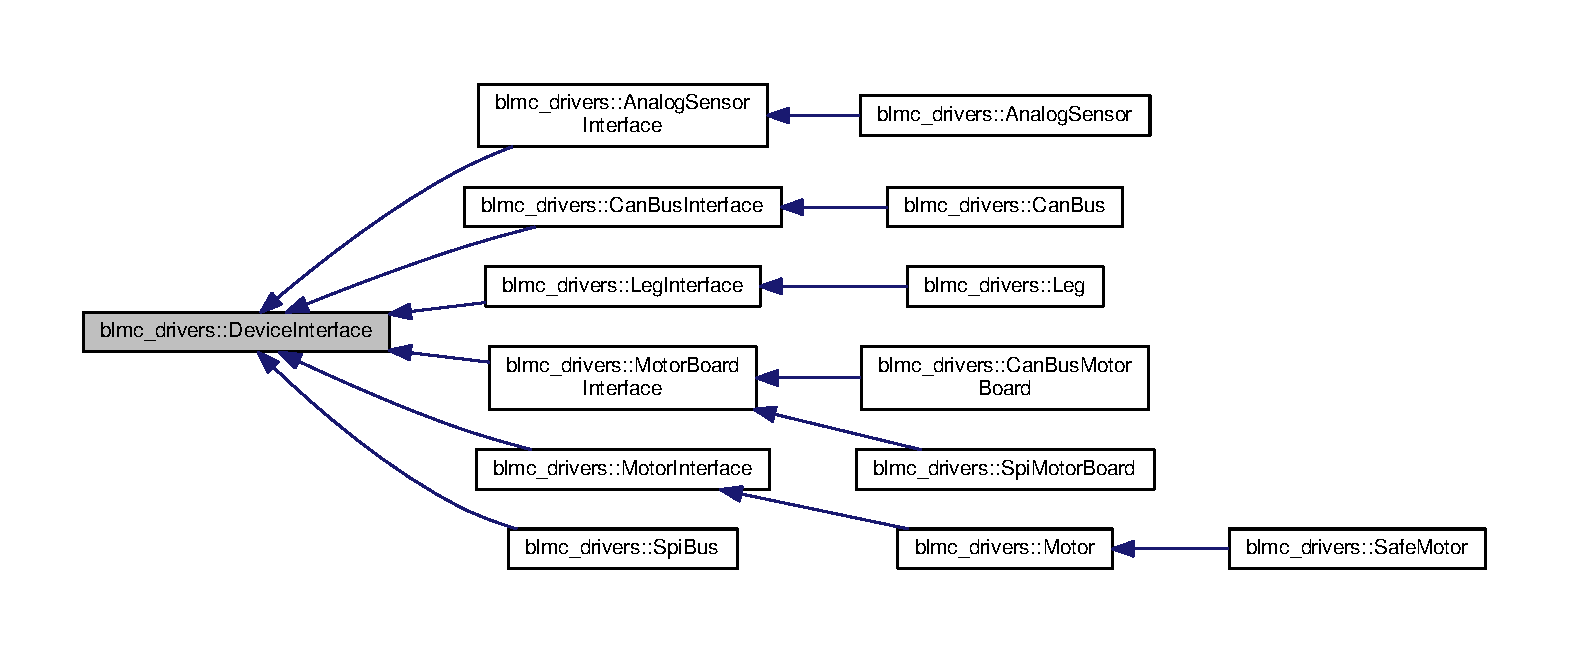
\includegraphics[width=350pt]{classblmc__drivers_1_1DeviceInterface__inherit__graph}
\end{center}
\end{figure}


\subsection{Detailed Description}
this class exists purely for logical reasons, it does not in itself implement anything. 

the purpose of this class is to provide guidelines how a device should be implemented. any device has a number of inputs and outputs, see the following diagram for an example with two inputs and outputs.  generally, we expect the following functions to be implemented\+:
\begin{DoxyItemize}
\item a set function for each input (several inputs may share a set function which takes an index argument).
\item a send\+\_\+if\+\_\+input\+\_\+changed() function which will send the inputs to the device if any of them have changed.
\item functions to access the current inputs and outputs, as well as the inputs which have been sent to the device. rather than just returning the latest elements, these function should return a Threadsafe\+Timeseries of these objects, such that the user can synchronize (e.\+g. wait for the next element or step through them one by one such that none of them is missed) 
\end{DoxyItemize}

The documentation for this class was generated from the following file\+:\begin{DoxyCompactItemize}
\item 
include/blmc\+\_\+drivers/devices/\hyperlink{device__interface_8hpp}{device\+\_\+interface.\+hpp}\end{DoxyCompactItemize}

\hypertarget{structHardware}{}\section{Hardware Struct Reference}
\label{structHardware}\index{Hardware@{Hardware}}
\subsection*{Public Attributes}
\begin{DoxyCompactItemize}
\item 
std\+::shared\+\_\+ptr$<$ \hyperlink{classblmc__drivers_1_1CanBusInterface}{blmc\+\_\+drivers\+::\+Can\+Bus\+Interface} $>$ {\bfseries can\+\_\+bus}\hypertarget{structHardware_af6014d03d5d50bacf8c96e841cf8184d}{}\label{structHardware_af6014d03d5d50bacf8c96e841cf8184d}

\item 
std\+::shared\+\_\+ptr$<$ \hyperlink{classblmc__drivers_1_1MotorBoardInterface}{blmc\+\_\+drivers\+::\+Motor\+Board\+Interface} $>$ {\bfseries motor\+\_\+board}\hypertarget{structHardware_a6882a74056ffaa2a946b0f9b98d00b02}{}\label{structHardware_a6882a74056ffaa2a946b0f9b98d00b02}

\item 
std\+::shared\+\_\+ptr$<$ \hyperlink{classblmc__drivers_1_1MotorInterface}{blmc\+\_\+drivers\+::\+Motor\+Interface} $>$ {\bfseries motor}\hypertarget{structHardware_a78675cea76da541862144708a3996dcc}{}\label{structHardware_a78675cea76da541862144708a3996dcc}

\item 
std\+::shared\+\_\+ptr$<$ \hyperlink{classblmc__drivers_1_1AnalogSensorInterface}{blmc\+\_\+drivers\+::\+Analog\+Sensor\+Interface} $>$ {\bfseries slider}\hypertarget{structHardware_ac10da22a00e796b078624795da7e835d}{}\label{structHardware_ac10da22a00e796b078624795da7e835d}

\end{DoxyCompactItemize}


The documentation for this struct was generated from the following files\+:\begin{DoxyCompactItemize}
\item 
demos/\hyperlink{demo__1__motor_8cpp}{demo\+\_\+1\+\_\+motor.\+cpp}\item 
demos/\hyperlink{demo__1__motor__print__everything_8cpp}{demo\+\_\+1\+\_\+motor\+\_\+print\+\_\+everything.\+cpp}\end{DoxyCompactItemize}

\hypertarget{classblmc__drivers_1_1Leg}{}\section{blmc\+\_\+drivers\+:\+:Leg Class Reference}
\label{classblmc__drivers_1_1Leg}\index{blmc\+\_\+drivers\+::\+Leg@{blmc\+\_\+drivers\+::\+Leg}}


The leg class is the implementation of the \hyperlink{classblmc__drivers_1_1LegInterface}{Leg\+Interface}.  




{\ttfamily \#include $<$leg.\+hpp$>$}



Inheritance diagram for blmc\+\_\+drivers\+:\+:Leg\+:
\nopagebreak
\begin{figure}[H]
\begin{center}
\leavevmode
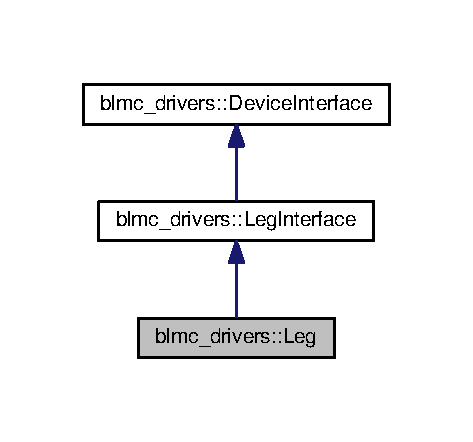
\includegraphics[width=227pt]{classblmc__drivers_1_1Leg__inherit__graph}
\end{center}
\end{figure}


Collaboration diagram for blmc\+\_\+drivers\+:\+:Leg\+:
\nopagebreak
\begin{figure}[H]
\begin{center}
\leavevmode
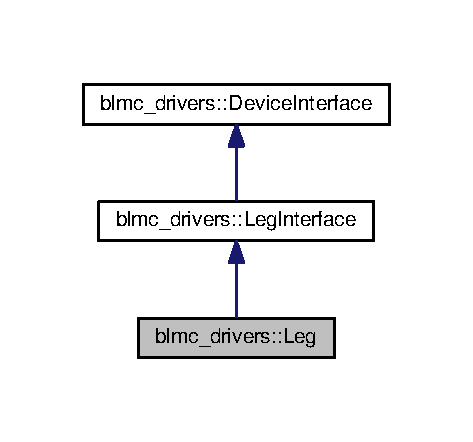
\includegraphics[width=227pt]{classblmc__drivers_1_1Leg__coll__graph}
\end{center}
\end{figure}
\subsection*{Public Member Functions}
\begin{DoxyCompactItemize}
\item 
\hyperlink{classblmc__drivers_1_1Leg_aaa53f0583fcfd7f4e8aa32889aaa2f85}{Leg} (std\+::shared\+\_\+ptr$<$ \hyperlink{classblmc__drivers_1_1MotorInterface}{Motor\+Interface} $>$ hip\+\_\+motor, std\+::shared\+\_\+ptr$<$ \hyperlink{classblmc__drivers_1_1MotorInterface}{Motor\+Interface} $>$ knee\+\_\+motor)
\begin{DoxyCompactList}\small\item\em Construct a new \hyperlink{classblmc__drivers_1_1Leg}{Leg} object. \end{DoxyCompactList}\item 
virtual \hyperlink{classblmc__drivers_1_1Leg_add76148d01d09ecb505bb23ce34d45c8}{$\sim$\+Leg} ()\hypertarget{classblmc__drivers_1_1Leg_add76148d01d09ecb505bb23ce34d45c8}{}\label{classblmc__drivers_1_1Leg_add76148d01d09ecb505bb23ce34d45c8}

\begin{DoxyCompactList}\small\item\em Destroy the \hyperlink{classblmc__drivers_1_1Leg}{Leg} object. \end{DoxyCompactList}\item 
virtual \hyperlink{classblmc__drivers_1_1LegInterface_ac5af9e6514abff5ee918813925a8e42d}{Ptr}$<$ const \hyperlink{classblmc__drivers_1_1LegInterface_a57a35b64a76fb4225637828d1b1c35a6}{Scalar\+Timeseries} $>$ \hyperlink{classblmc__drivers_1_1Leg_a585436aebc39562a5d1a486810b8b9ce}{get\+\_\+motor\+\_\+measurement} (const int \&motor\+\_\+index, const int \&measurement\+\_\+index) const 
\begin{DoxyCompactList}\small\item\em Getters. \end{DoxyCompactList}\item 
virtual \hyperlink{classblmc__drivers_1_1LegInterface_ac5af9e6514abff5ee918813925a8e42d}{Ptr}$<$ const \hyperlink{classblmc__drivers_1_1LegInterface_a57a35b64a76fb4225637828d1b1c35a6}{Scalar\+Timeseries} $>$ \hyperlink{classblmc__drivers_1_1Leg_af4428c8734c5b393df8072a14850d9b1}{get\+\_\+current\+\_\+target} (const int \&motor\+\_\+index) const 
\begin{DoxyCompactList}\small\item\em Get the actual target current. \end{DoxyCompactList}\item 
virtual \hyperlink{classblmc__drivers_1_1LegInterface_ac5af9e6514abff5ee918813925a8e42d}{Ptr}$<$ const \hyperlink{classblmc__drivers_1_1LegInterface_a57a35b64a76fb4225637828d1b1c35a6}{Scalar\+Timeseries} $>$ \hyperlink{classblmc__drivers_1_1Leg_a353253074a39f566055121c2cb4adc6a}{get\+\_\+sent\+\_\+current\+\_\+target} (const int \&motor\+\_\+index) const 
\begin{DoxyCompactList}\small\item\em Get the last sent target current. \end{DoxyCompactList}\item 
virtual void \hyperlink{classblmc__drivers_1_1Leg_a05415969ef111f86837b34bdaecb7320}{set\+\_\+current\+\_\+target} (const double \&current\+\_\+target, const int \&motor\+\_\+index)\hypertarget{classblmc__drivers_1_1Leg_a05415969ef111f86837b34bdaecb7320}{}\label{classblmc__drivers_1_1Leg_a05415969ef111f86837b34bdaecb7320}

\begin{DoxyCompactList}\small\item\em setters ================================================================ \end{DoxyCompactList}\item 
virtual void \hyperlink{classblmc__drivers_1_1Leg_a82bb681e4c5047babf699cff559e9488}{send\+\_\+if\+\_\+input\+\_\+changed} ()\hypertarget{classblmc__drivers_1_1Leg_a82bb681e4c5047babf699cff559e9488}{}\label{classblmc__drivers_1_1Leg_a82bb681e4c5047babf699cff559e9488}

\begin{DoxyCompactList}\small\item\em sender ================================================================= \end{DoxyCompactList}\end{DoxyCompactItemize}
\subsection*{Private Attributes}
\begin{DoxyCompactItemize}
\item 
std\+::array$<$ std\+::shared\+\_\+ptr$<$ \hyperlink{classblmc__drivers_1_1MotorInterface}{Motor\+Interface} $>$, 2 $>$ \hyperlink{classblmc__drivers_1_1Leg_a78289d4c19fc35dbc3e7dd849e57479e}{motors\+\_\+}
\begin{DoxyCompactList}\small\item\em ======================================================================== \end{DoxyCompactList}\end{DoxyCompactItemize}
\subsection*{Additional Inherited Members}


\subsection{Detailed Description}
The leg class is the implementation of the \hyperlink{classblmc__drivers_1_1LegInterface}{Leg\+Interface}. 

This is the decalartion and the definition of the class as it is very simple. 

\subsection{Constructor \& Destructor Documentation}
\index{blmc\+\_\+drivers\+::\+Leg@{blmc\+\_\+drivers\+::\+Leg}!Leg@{Leg}}
\index{Leg@{Leg}!blmc\+\_\+drivers\+::\+Leg@{blmc\+\_\+drivers\+::\+Leg}}
\subsubsection[{\texorpdfstring{Leg(std\+::shared\+\_\+ptr$<$ Motor\+Interface $>$ hip\+\_\+motor, std\+::shared\+\_\+ptr$<$ Motor\+Interface $>$ knee\+\_\+motor)}{Leg(std::shared_ptr< MotorInterface > hip_motor, std::shared_ptr< MotorInterface > knee_motor)}}]{\setlength{\rightskip}{0pt plus 5cm}blmc\+\_\+drivers\+::\+Leg\+::\+Leg (
\begin{DoxyParamCaption}
\item[{std\+::shared\+\_\+ptr$<$ {\bf Motor\+Interface} $>$}]{hip\+\_\+motor, }
\item[{std\+::shared\+\_\+ptr$<$ {\bf Motor\+Interface} $>$}]{knee\+\_\+motor}
\end{DoxyParamCaption}
)\hspace{0.3cm}{\ttfamily [inline]}}\hypertarget{classblmc__drivers_1_1Leg_aaa53f0583fcfd7f4e8aa32889aaa2f85}{}\label{classblmc__drivers_1_1Leg_aaa53f0583fcfd7f4e8aa32889aaa2f85}


Construct a new \hyperlink{classblmc__drivers_1_1Leg}{Leg} object. 


\begin{DoxyParams}{Parameters}
{\em hip\+\_\+motor} & is the pointer to the hip motor \\
\hline
{\em knee\+\_\+motor} & is the pointer to the knee motor \\
\hline
\end{DoxyParams}


\subsection{Member Function Documentation}
\index{blmc\+\_\+drivers\+::\+Leg@{blmc\+\_\+drivers\+::\+Leg}!get\+\_\+current\+\_\+target@{get\+\_\+current\+\_\+target}}
\index{get\+\_\+current\+\_\+target@{get\+\_\+current\+\_\+target}!blmc\+\_\+drivers\+::\+Leg@{blmc\+\_\+drivers\+::\+Leg}}
\subsubsection[{\texorpdfstring{get\+\_\+current\+\_\+target(const int \&motor\+\_\+index) const }{get_current_target(const int &motor_index) const }}]{\setlength{\rightskip}{0pt plus 5cm}virtual {\bf Ptr}$<$const {\bf Scalar\+Timeseries}$>$ blmc\+\_\+drivers\+::\+Leg\+::get\+\_\+current\+\_\+target (
\begin{DoxyParamCaption}
\item[{const int \&}]{motor\+\_\+index}
\end{DoxyParamCaption}
) const\hspace{0.3cm}{\ttfamily [inline]}, {\ttfamily [virtual]}}\hypertarget{classblmc__drivers_1_1Leg_af4428c8734c5b393df8072a14850d9b1}{}\label{classblmc__drivers_1_1Leg_af4428c8734c5b393df8072a14850d9b1}


Get the actual target current. 


\begin{DoxyParams}[1]{Parameters}
\mbox{\tt in}  & {\em motor\+\_\+index} & designate the motor from which we want the data from. \\
\hline
\end{DoxyParams}
\begin{DoxyReturn}{Returns}
Ptr$<$const Scalar\+Timeseries$>$ is the list of the lasts time stamped acquiered. 
\end{DoxyReturn}


Implements \hyperlink{classblmc__drivers_1_1LegInterface_a44bac5c9a6015f0e08370b3bc9957512}{blmc\+\_\+drivers\+::\+Leg\+Interface}.

\index{blmc\+\_\+drivers\+::\+Leg@{blmc\+\_\+drivers\+::\+Leg}!get\+\_\+motor\+\_\+measurement@{get\+\_\+motor\+\_\+measurement}}
\index{get\+\_\+motor\+\_\+measurement@{get\+\_\+motor\+\_\+measurement}!blmc\+\_\+drivers\+::\+Leg@{blmc\+\_\+drivers\+::\+Leg}}
\subsubsection[{\texorpdfstring{get\+\_\+motor\+\_\+measurement(const int \&motor\+\_\+index, const int \&measurement\+\_\+index) const }{get_motor_measurement(const int &motor_index, const int &measurement_index) const }}]{\setlength{\rightskip}{0pt plus 5cm}virtual {\bf Ptr}$<$const {\bf Scalar\+Timeseries}$>$ blmc\+\_\+drivers\+::\+Leg\+::get\+\_\+motor\+\_\+measurement (
\begin{DoxyParamCaption}
\item[{const int \&}]{motor\+\_\+index, }
\item[{const int \&}]{measurement\+\_\+index}
\end{DoxyParamCaption}
) const\hspace{0.3cm}{\ttfamily [inline]}, {\ttfamily [virtual]}}\hypertarget{classblmc__drivers_1_1Leg_a585436aebc39562a5d1a486810b8b9ce}{}\label{classblmc__drivers_1_1Leg_a585436aebc39562a5d1a486810b8b9ce}


Getters. 

Get the motor measurements.


\begin{DoxyParams}{Parameters}
{\em motor\+\_\+index} & \\
\hline
{\em measurement\+\_\+index} & \\
\hline
\end{DoxyParams}
\begin{DoxyReturn}{Returns}
Ptr$<$const Scalar\+Timeseries$>$ 
\end{DoxyReturn}


Implements \hyperlink{classblmc__drivers_1_1LegInterface_ae653c7ee0ab7aa9d16a6bfce01580200}{blmc\+\_\+drivers\+::\+Leg\+Interface}.

\index{blmc\+\_\+drivers\+::\+Leg@{blmc\+\_\+drivers\+::\+Leg}!get\+\_\+sent\+\_\+current\+\_\+target@{get\+\_\+sent\+\_\+current\+\_\+target}}
\index{get\+\_\+sent\+\_\+current\+\_\+target@{get\+\_\+sent\+\_\+current\+\_\+target}!blmc\+\_\+drivers\+::\+Leg@{blmc\+\_\+drivers\+::\+Leg}}
\subsubsection[{\texorpdfstring{get\+\_\+sent\+\_\+current\+\_\+target(const int \&motor\+\_\+index) const }{get_sent_current_target(const int &motor_index) const }}]{\setlength{\rightskip}{0pt plus 5cm}virtual {\bf Ptr}$<$const {\bf Scalar\+Timeseries}$>$ blmc\+\_\+drivers\+::\+Leg\+::get\+\_\+sent\+\_\+current\+\_\+target (
\begin{DoxyParamCaption}
\item[{const int \&}]{motor\+\_\+index}
\end{DoxyParamCaption}
) const\hspace{0.3cm}{\ttfamily [inline]}, {\ttfamily [virtual]}}\hypertarget{classblmc__drivers_1_1Leg_a353253074a39f566055121c2cb4adc6a}{}\label{classblmc__drivers_1_1Leg_a353253074a39f566055121c2cb4adc6a}


Get the last sent target current. 


\begin{DoxyParams}[1]{Parameters}
\mbox{\tt in}  & {\em motor\+\_\+index} & designate the motor from which we want the data from. \\
\hline
\end{DoxyParams}
\begin{DoxyReturn}{Returns}
Ptr$<$const Scalar\+Timeseries$>$ is the list of the lasts time stamped acquiered. 
\end{DoxyReturn}


Implements \hyperlink{classblmc__drivers_1_1LegInterface_ab724283c8eeadca0e7b8829de64f4f44}{blmc\+\_\+drivers\+::\+Leg\+Interface}.



\subsection{Member Data Documentation}
\index{blmc\+\_\+drivers\+::\+Leg@{blmc\+\_\+drivers\+::\+Leg}!motors\+\_\+@{motors\+\_\+}}
\index{motors\+\_\+@{motors\+\_\+}!blmc\+\_\+drivers\+::\+Leg@{blmc\+\_\+drivers\+::\+Leg}}
\subsubsection[{\texorpdfstring{motors\+\_\+}{motors_}}]{\setlength{\rightskip}{0pt plus 5cm}std\+::array$<$std\+::shared\+\_\+ptr$<${\bf Motor\+Interface}$>$, 2$>$ blmc\+\_\+drivers\+::\+Leg\+::motors\+\_\+\hspace{0.3cm}{\ttfamily [private]}}\hypertarget{classblmc__drivers_1_1Leg_a78289d4c19fc35dbc3e7dd849e57479e}{}\label{classblmc__drivers_1_1Leg_a78289d4c19fc35dbc3e7dd849e57479e}


======================================================================== 

This list contains pointers to two motors. This motors are respectively the hip and the knee of the leg. 

The documentation for this class was generated from the following file\+:\begin{DoxyCompactItemize}
\item 
include/blmc\+\_\+drivers/devices/\hyperlink{leg_8hpp}{leg.\+hpp}\end{DoxyCompactItemize}

\hypertarget{classLegController}{}\section{Leg\+Controller Class Reference}
\label{classLegController}\index{Leg\+Controller@{Leg\+Controller}}


Simple PD control on the leg.  


\subsection*{Public Member Functions}
\begin{DoxyCompactItemize}
\item 
\hyperlink{classLegController_a9d1253c4c70fe6b83e449830c7328b58}{Leg\+Controller} (std\+::shared\+\_\+ptr$<$ \hyperlink{classblmc__drivers_1_1Leg}{blmc\+\_\+drivers\+::\+Leg} $>$ leg, std\+::shared\+\_\+ptr$<$ \hyperlink{classblmc__drivers_1_1AnalogSensor}{blmc\+\_\+drivers\+::\+Analog\+Sensor} $>$ analog\+\_\+sensor)
\begin{DoxyCompactList}\small\item\em Construct a new \hyperlink{classLegController}{Leg\+Controller} object. \end{DoxyCompactList}\item 
\hyperlink{classLegController_ad7f3068767ed754bbefd1744463764d0}{$\sim$\+Leg\+Controller} ()\hypertarget{classLegController_ad7f3068767ed754bbefd1744463764d0}{}\label{classLegController_ad7f3068767ed754bbefd1744463764d0}

\begin{DoxyCompactList}\small\item\em Destroy the \hyperlink{classLegController}{Leg\+Controller} object. \end{DoxyCompactList}\item 
void \hyperlink{classLegController_adacfe6a1709021da8cd7009672d01440}{start\+\_\+loop} ()\hypertarget{classLegController_adacfe6a1709021da8cd7009672d01440}{}\label{classLegController_adacfe6a1709021da8cd7009672d01440}

\begin{DoxyCompactList}\small\item\em helper to strat the real time thread. \end{DoxyCompactList}\end{DoxyCompactItemize}
\subsection*{Static Public Member Functions}
\begin{DoxyCompactItemize}
\item 
static T\+H\+R\+E\+A\+D\+\_\+\+F\+U\+N\+C\+T\+I\+O\+N\+\_\+\+R\+E\+T\+U\+R\+N\+\_\+\+T\+Y\+PE \hyperlink{classLegController_a87bba6942e6f8ba649f595e871d0d379}{loop} (void $\ast$instance\+\_\+pointer)\hypertarget{classLegController_a87bba6942e6f8ba649f595e871d0d379}{}\label{classLegController_a87bba6942e6f8ba649f595e871d0d379}

\begin{DoxyCompactList}\small\item\em this function is just a wrapper around the actual loop function, such that it can be spawned as a posix thread. \end{DoxyCompactList}\end{DoxyCompactItemize}
\subsection*{Private Member Functions}
\begin{DoxyCompactItemize}
\item 
void \hyperlink{classLegController_a00000dd7bbaa4f1e05a9ea16f05e73e8}{loop} ()
\begin{DoxyCompactList}\small\item\em this is a simple control loop which runs at a kilohertz. \end{DoxyCompactList}\end{DoxyCompactItemize}
\subsection*{Private Attributes}
\begin{DoxyCompactItemize}
\item 
std\+::shared\+\_\+ptr$<$ \hyperlink{classblmc__drivers_1_1Leg}{blmc\+\_\+drivers\+::\+Leg} $>$ \hyperlink{classLegController_af2abd6d8c18c9653813bb231a0688a54}{leg\+\_\+}\hypertarget{classLegController_af2abd6d8c18c9653813bb231a0688a54}{}\label{classLegController_af2abd6d8c18c9653813bb231a0688a54}

\begin{DoxyCompactList}\small\item\em is the leg to control \end{DoxyCompactList}\item 
std\+::shared\+\_\+ptr$<$ \hyperlink{classblmc__drivers_1_1AnalogSensor}{blmc\+\_\+drivers\+::\+Analog\+Sensor} $>$ \hyperlink{classLegController_a1a05529b6f3f40c7d3da6e6a9fa94cea}{analog\+\_\+sensor\+\_\+}\hypertarget{classLegController_a1a05529b6f3f40c7d3da6e6a9fa94cea}{}\label{classLegController_a1a05529b6f3f40c7d3da6e6a9fa94cea}

\begin{DoxyCompactList}\small\item\em is the list of sliders \end{DoxyCompactList}\item 
real\+\_\+time\+\_\+tools\+::\+Real\+Time\+Thread \hyperlink{classLegController_a34aac27ee8efb204f98203b553094588}{rt\+\_\+thread\+\_\+}\hypertarget{classLegController_a34aac27ee8efb204f98203b553094588}{}\label{classLegController_a34aac27ee8efb204f98203b553094588}

\begin{DoxyCompactList}\small\item\em is the real time thread object. \end{DoxyCompactList}\item 
bool \hyperlink{classLegController_a991995e57f3581074b9c0eec32966e35}{stop\+\_\+loop\+\_\+}\hypertarget{classLegController_a991995e57f3581074b9c0eec32966e35}{}\label{classLegController_a991995e57f3581074b9c0eec32966e35}

\begin{DoxyCompactList}\small\item\em manages the shutdown of the controller \end{DoxyCompactList}\end{DoxyCompactItemize}


\subsection{Detailed Description}
Simple PD control on the leg. 

\subsection{Constructor \& Destructor Documentation}
\index{Leg\+Controller@{Leg\+Controller}!Leg\+Controller@{Leg\+Controller}}
\index{Leg\+Controller@{Leg\+Controller}!Leg\+Controller@{Leg\+Controller}}
\subsubsection[{\texorpdfstring{Leg\+Controller(std\+::shared\+\_\+ptr$<$ blmc\+\_\+drivers\+::\+Leg $>$ leg, std\+::shared\+\_\+ptr$<$ blmc\+\_\+drivers\+::\+Analog\+Sensor $>$ analog\+\_\+sensor)}{LegController(std::shared_ptr< blmc_drivers::Leg > leg, std::shared_ptr< blmc_drivers::AnalogSensor > analog_sensor)}}]{\setlength{\rightskip}{0pt plus 5cm}Leg\+Controller\+::\+Leg\+Controller (
\begin{DoxyParamCaption}
\item[{std\+::shared\+\_\+ptr$<$ {\bf blmc\+\_\+drivers\+::\+Leg} $>$}]{leg, }
\item[{std\+::shared\+\_\+ptr$<$ {\bf blmc\+\_\+drivers\+::\+Analog\+Sensor} $>$}]{analog\+\_\+sensor}
\end{DoxyParamCaption}
)\hspace{0.3cm}{\ttfamily [inline]}}\hypertarget{classLegController_a9d1253c4c70fe6b83e449830c7328b58}{}\label{classLegController_a9d1253c4c70fe6b83e449830c7328b58}


Construct a new \hyperlink{classLegController}{Leg\+Controller} object. 


\begin{DoxyParams}{Parameters}
{\em leg} & \\
\hline
{\em analog\+\_\+sensor} & \\
\hline
\end{DoxyParams}


\subsection{Member Function Documentation}
\index{Leg\+Controller@{Leg\+Controller}!loop@{loop}}
\index{loop@{loop}!Leg\+Controller@{Leg\+Controller}}
\subsubsection[{\texorpdfstring{loop()}{loop()}}]{\setlength{\rightskip}{0pt plus 5cm}void Leg\+Controller\+::loop (
\begin{DoxyParamCaption}
{}
\end{DoxyParamCaption}
)\hspace{0.3cm}{\ttfamily [inline]}, {\ttfamily [private]}}\hypertarget{classLegController_a00000dd7bbaa4f1e05a9ea16f05e73e8}{}\label{classLegController_a00000dd7bbaa4f1e05a9ea16f05e73e8}


this is a simple control loop which runs at a kilohertz. 

it reads the measurement from the analog sensor, in this case the slider. then it scales it and sends it as the current target to the motor. 

The documentation for this class was generated from the following file\+:\begin{DoxyCompactItemize}
\item 
demos/\hyperlink{demo__leg_8cpp}{demo\+\_\+leg.\+cpp}\end{DoxyCompactItemize}

\hypertarget{classblmc__drivers_1_1LegInterface}{}\section{blmc\+\_\+drivers\+:\+:Leg\+Interface Class Reference}
\label{classblmc__drivers_1_1LegInterface}\index{blmc\+\_\+drivers\+::\+Leg\+Interface@{blmc\+\_\+drivers\+::\+Leg\+Interface}}


This class defines an interface to control a leg.  




{\ttfamily \#include $<$leg.\+hpp$>$}



Inheritance diagram for blmc\+\_\+drivers\+:\+:Leg\+Interface\+:
\nopagebreak
\begin{figure}[H]
\begin{center}
\leavevmode
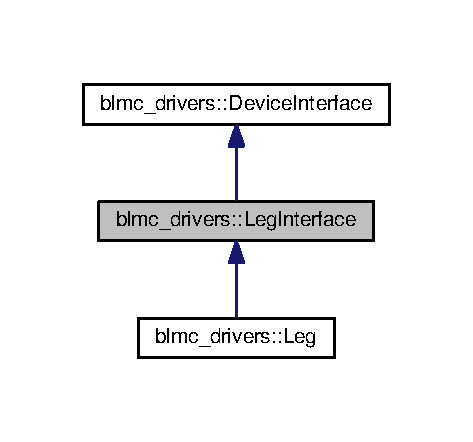
\includegraphics[width=227pt]{classblmc__drivers_1_1LegInterface__inherit__graph}
\end{center}
\end{figure}


Collaboration diagram for blmc\+\_\+drivers\+:\+:Leg\+Interface\+:
\nopagebreak
\begin{figure}[H]
\begin{center}
\leavevmode
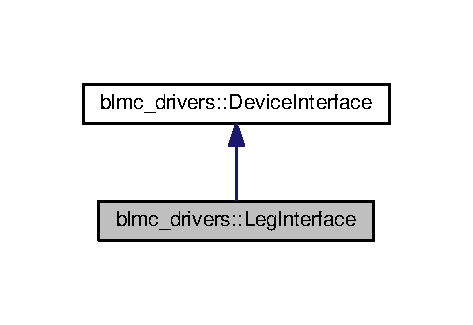
\includegraphics[width=227pt]{classblmc__drivers_1_1LegInterface__coll__graph}
\end{center}
\end{figure}
\subsection*{Public Types}
\begin{DoxyCompactItemize}
\item 
enum \hyperlink{classblmc__drivers_1_1LegInterface_a9335cf8bf2595f70716159927d927346}{Motor\+Measurement\+Indexing} \{ \\*
{\bfseries current}, 
{\bfseries position}, 
{\bfseries velocity}, 
{\bfseries encoder\+\_\+index}, 
\\*
{\bfseries motor\+\_\+measurement\+\_\+count}
 \}\hypertarget{classblmc__drivers_1_1LegInterface_a9335cf8bf2595f70716159927d927346}{}\label{classblmc__drivers_1_1LegInterface_a9335cf8bf2595f70716159927d927346}
\begin{DoxyCompactList}\small\item\em Motor\+Measurement\+Indexing this enum allow to access the different kind of sensor measurements in an understandable way in the code. \end{DoxyCompactList}
\item 
enum \hyperlink{classblmc__drivers_1_1LegInterface_a2a11567617debfdb731ac06e2938712c}{Motor\+Indexing} \{ {\bfseries hip}, 
{\bfseries knee}, 
{\bfseries motor\+\_\+count}
 \}\hypertarget{classblmc__drivers_1_1LegInterface_a2a11567617debfdb731ac06e2938712c}{}\label{classblmc__drivers_1_1LegInterface_a2a11567617debfdb731ac06e2938712c}
\begin{DoxyCompactList}\small\item\em This enum list the motors in the leg. \end{DoxyCompactList}
\item 
typedef real\+\_\+time\+\_\+tools\+::\+Threadsafe\+Timeseries$<$ double $>$ \hyperlink{classblmc__drivers_1_1LegInterface_a57a35b64a76fb4225637828d1b1c35a6}{Scalar\+Timeseries}\hypertarget{classblmc__drivers_1_1LegInterface_a57a35b64a76fb4225637828d1b1c35a6}{}\label{classblmc__drivers_1_1LegInterface_a57a35b64a76fb4225637828d1b1c35a6}

\begin{DoxyCompactList}\small\item\em Scalar\+Timeseries is a simple shortcut for more intelligible code. \end{DoxyCompactList}\item 
{\footnotesize template$<$typename Type $>$ }\\using \hyperlink{classblmc__drivers_1_1LegInterface_ac5af9e6514abff5ee918813925a8e42d}{Ptr} = std\+::shared\+\_\+ptr$<$ Type $>$
\begin{DoxyCompactList}\small\item\em This is a shortcut for creating shared pointer in a simpler writting expression. \end{DoxyCompactList}\end{DoxyCompactItemize}
\subsection*{Public Member Functions}
\begin{DoxyCompactItemize}
\item 
virtual \hyperlink{classblmc__drivers_1_1LegInterface_afe46102b0ce1c790e921d71f86868066}{$\sim$\+Leg\+Interface} ()\hypertarget{classblmc__drivers_1_1LegInterface_afe46102b0ce1c790e921d71f86868066}{}\label{classblmc__drivers_1_1LegInterface_afe46102b0ce1c790e921d71f86868066}

\begin{DoxyCompactList}\small\item\em Destroy the \hyperlink{classblmc__drivers_1_1LegInterface}{Leg\+Interface} object. \end{DoxyCompactList}\item 
virtual \hyperlink{classblmc__drivers_1_1LegInterface_ac5af9e6514abff5ee918813925a8e42d}{Ptr}$<$ const \hyperlink{classblmc__drivers_1_1LegInterface_a57a35b64a76fb4225637828d1b1c35a6}{Scalar\+Timeseries} $>$ \hyperlink{classblmc__drivers_1_1LegInterface_ae653c7ee0ab7aa9d16a6bfce01580200}{get\+\_\+motor\+\_\+measurement} (const int \&motor\+\_\+index, const int \&measurement\+\_\+index) const =0
\begin{DoxyCompactList}\small\item\em Getters. \end{DoxyCompactList}\item 
virtual \hyperlink{classblmc__drivers_1_1LegInterface_ac5af9e6514abff5ee918813925a8e42d}{Ptr}$<$ const \hyperlink{classblmc__drivers_1_1LegInterface_a57a35b64a76fb4225637828d1b1c35a6}{Scalar\+Timeseries} $>$ \hyperlink{classblmc__drivers_1_1LegInterface_a44bac5c9a6015f0e08370b3bc9957512}{get\+\_\+current\+\_\+target} (const int \&motor\+\_\+index) const =0
\begin{DoxyCompactList}\small\item\em Get the actual target current. \end{DoxyCompactList}\item 
virtual \hyperlink{classblmc__drivers_1_1LegInterface_ac5af9e6514abff5ee918813925a8e42d}{Ptr}$<$ const \hyperlink{classblmc__drivers_1_1LegInterface_a57a35b64a76fb4225637828d1b1c35a6}{Scalar\+Timeseries} $>$ \hyperlink{classblmc__drivers_1_1LegInterface_ab724283c8eeadca0e7b8829de64f4f44}{get\+\_\+sent\+\_\+current\+\_\+target} (const int \&motor\+\_\+index) const =0
\begin{DoxyCompactList}\small\item\em Get the last sent target current. \end{DoxyCompactList}\item 
virtual void \hyperlink{classblmc__drivers_1_1LegInterface_a6917a158f12589c9ee6aa45304fdafce}{set\+\_\+current\+\_\+target} (const double \&current\+\_\+target, const int \&motor\+\_\+index)=0
\begin{DoxyCompactList}\small\item\em Setters. \end{DoxyCompactList}\item 
virtual void \hyperlink{classblmc__drivers_1_1LegInterface_aaf3d3759b63a3ffe7e9cee360302f9b7}{send\+\_\+if\+\_\+input\+\_\+changed} ()=0
\begin{DoxyCompactList}\small\item\em Sender. \end{DoxyCompactList}\end{DoxyCompactItemize}


\subsection{Detailed Description}
This class defines an interface to control a leg. 

This legg is composed of 2 motor, one for the hip and one for the knee. 

\subsection{Member Typedef Documentation}
\index{blmc\+\_\+drivers\+::\+Leg\+Interface@{blmc\+\_\+drivers\+::\+Leg\+Interface}!Ptr@{Ptr}}
\index{Ptr@{Ptr}!blmc\+\_\+drivers\+::\+Leg\+Interface@{blmc\+\_\+drivers\+::\+Leg\+Interface}}
\subsubsection[{\texorpdfstring{Ptr}{Ptr}}]{\setlength{\rightskip}{0pt plus 5cm}template$<$typename Type $>$ using {\bf blmc\+\_\+drivers\+::\+Leg\+Interface\+::\+Ptr} =  std\+::shared\+\_\+ptr$<$Type$>$}\hypertarget{classblmc__drivers_1_1LegInterface_ac5af9e6514abff5ee918813925a8e42d}{}\label{classblmc__drivers_1_1LegInterface_ac5af9e6514abff5ee918813925a8e42d}


This is a shortcut for creating shared pointer in a simpler writting expression. 


\begin{DoxyTemplParams}{Template Parameters}
{\em Type} & is the template paramer of the shared pointer. \\
\hline
\end{DoxyTemplParams}


\subsection{Member Function Documentation}
\index{blmc\+\_\+drivers\+::\+Leg\+Interface@{blmc\+\_\+drivers\+::\+Leg\+Interface}!get\+\_\+current\+\_\+target@{get\+\_\+current\+\_\+target}}
\index{get\+\_\+current\+\_\+target@{get\+\_\+current\+\_\+target}!blmc\+\_\+drivers\+::\+Leg\+Interface@{blmc\+\_\+drivers\+::\+Leg\+Interface}}
\subsubsection[{\texorpdfstring{get\+\_\+current\+\_\+target(const int \&motor\+\_\+index) const =0}{get_current_target(const int &motor_index) const =0}}]{\setlength{\rightskip}{0pt plus 5cm}virtual {\bf Ptr}$<$const {\bf Scalar\+Timeseries}$>$ blmc\+\_\+drivers\+::\+Leg\+Interface\+::get\+\_\+current\+\_\+target (
\begin{DoxyParamCaption}
\item[{const int \&}]{motor\+\_\+index}
\end{DoxyParamCaption}
) const\hspace{0.3cm}{\ttfamily [pure virtual]}}\hypertarget{classblmc__drivers_1_1LegInterface_a44bac5c9a6015f0e08370b3bc9957512}{}\label{classblmc__drivers_1_1LegInterface_a44bac5c9a6015f0e08370b3bc9957512}


Get the actual target current. 


\begin{DoxyParams}[1]{Parameters}
\mbox{\tt in}  & {\em motor\+\_\+index} & designate the motor from which we want the data from. \\
\hline
\end{DoxyParams}
\begin{DoxyReturn}{Returns}
Ptr$<$const Scalar\+Timeseries$>$ is the list of the lasts time stamped acquiered. 
\end{DoxyReturn}


Implemented in \hyperlink{classblmc__drivers_1_1Leg_af4428c8734c5b393df8072a14850d9b1}{blmc\+\_\+drivers\+::\+Leg}.

\index{blmc\+\_\+drivers\+::\+Leg\+Interface@{blmc\+\_\+drivers\+::\+Leg\+Interface}!get\+\_\+motor\+\_\+measurement@{get\+\_\+motor\+\_\+measurement}}
\index{get\+\_\+motor\+\_\+measurement@{get\+\_\+motor\+\_\+measurement}!blmc\+\_\+drivers\+::\+Leg\+Interface@{blmc\+\_\+drivers\+::\+Leg\+Interface}}
\subsubsection[{\texorpdfstring{get\+\_\+motor\+\_\+measurement(const int \&motor\+\_\+index, const int \&measurement\+\_\+index) const =0}{get_motor_measurement(const int &motor_index, const int &measurement_index) const =0}}]{\setlength{\rightskip}{0pt plus 5cm}virtual {\bf Ptr}$<$const {\bf Scalar\+Timeseries}$>$ blmc\+\_\+drivers\+::\+Leg\+Interface\+::get\+\_\+motor\+\_\+measurement (
\begin{DoxyParamCaption}
\item[{const int \&}]{motor\+\_\+index, }
\item[{const int \&}]{measurement\+\_\+index}
\end{DoxyParamCaption}
) const\hspace{0.3cm}{\ttfamily [pure virtual]}}\hypertarget{classblmc__drivers_1_1LegInterface_ae653c7ee0ab7aa9d16a6bfce01580200}{}\label{classblmc__drivers_1_1LegInterface_ae653c7ee0ab7aa9d16a6bfce01580200}


Getters. 

Get the device output


\begin{DoxyParams}[1]{Parameters}
\mbox{\tt in}  & {\em motor\+\_\+index} & designate the motor from which we want the data from. \\
\hline
\mbox{\tt in}  & {\em measurement\+\_\+index} & is teh kind of data we are looking for. \\
\hline
\end{DoxyParams}
\begin{DoxyReturn}{Returns}
Ptr$<$const Scalar\+Timeseries$>$ is the list of the lasts time stamped acquiered. 
\end{DoxyReturn}


Implemented in \hyperlink{classblmc__drivers_1_1Leg_a585436aebc39562a5d1a486810b8b9ce}{blmc\+\_\+drivers\+::\+Leg}.

\index{blmc\+\_\+drivers\+::\+Leg\+Interface@{blmc\+\_\+drivers\+::\+Leg\+Interface}!get\+\_\+sent\+\_\+current\+\_\+target@{get\+\_\+sent\+\_\+current\+\_\+target}}
\index{get\+\_\+sent\+\_\+current\+\_\+target@{get\+\_\+sent\+\_\+current\+\_\+target}!blmc\+\_\+drivers\+::\+Leg\+Interface@{blmc\+\_\+drivers\+::\+Leg\+Interface}}
\subsubsection[{\texorpdfstring{get\+\_\+sent\+\_\+current\+\_\+target(const int \&motor\+\_\+index) const =0}{get_sent_current_target(const int &motor_index) const =0}}]{\setlength{\rightskip}{0pt plus 5cm}virtual {\bf Ptr}$<$const {\bf Scalar\+Timeseries}$>$ blmc\+\_\+drivers\+::\+Leg\+Interface\+::get\+\_\+sent\+\_\+current\+\_\+target (
\begin{DoxyParamCaption}
\item[{const int \&}]{motor\+\_\+index}
\end{DoxyParamCaption}
) const\hspace{0.3cm}{\ttfamily [pure virtual]}}\hypertarget{classblmc__drivers_1_1LegInterface_ab724283c8eeadca0e7b8829de64f4f44}{}\label{classblmc__drivers_1_1LegInterface_ab724283c8eeadca0e7b8829de64f4f44}


Get the last sent target current. 


\begin{DoxyParams}[1]{Parameters}
\mbox{\tt in}  & {\em motor\+\_\+index} & designate the motor from which we want the data from. \\
\hline
\end{DoxyParams}
\begin{DoxyReturn}{Returns}
Ptr$<$const Scalar\+Timeseries$>$ is the list of the lasts time stamped acquiered. 
\end{DoxyReturn}


Implemented in \hyperlink{classblmc__drivers_1_1Leg_a353253074a39f566055121c2cb4adc6a}{blmc\+\_\+drivers\+::\+Leg}.

\index{blmc\+\_\+drivers\+::\+Leg\+Interface@{blmc\+\_\+drivers\+::\+Leg\+Interface}!send\+\_\+if\+\_\+input\+\_\+changed@{send\+\_\+if\+\_\+input\+\_\+changed}}
\index{send\+\_\+if\+\_\+input\+\_\+changed@{send\+\_\+if\+\_\+input\+\_\+changed}!blmc\+\_\+drivers\+::\+Leg\+Interface@{blmc\+\_\+drivers\+::\+Leg\+Interface}}
\subsubsection[{\texorpdfstring{send\+\_\+if\+\_\+input\+\_\+changed()=0}{send_if_input_changed()=0}}]{\setlength{\rightskip}{0pt plus 5cm}virtual void blmc\+\_\+drivers\+::\+Leg\+Interface\+::send\+\_\+if\+\_\+input\+\_\+changed (
\begin{DoxyParamCaption}
{}
\end{DoxyParamCaption}
)\hspace{0.3cm}{\ttfamily [pure virtual]}}\hypertarget{classblmc__drivers_1_1LegInterface_aaf3d3759b63a3ffe7e9cee360302f9b7}{}\label{classblmc__drivers_1_1LegInterface_aaf3d3759b63a3ffe7e9cee360302f9b7}


Sender. 

Actually send the target current to the motor cards. 

Implemented in \hyperlink{classblmc__drivers_1_1Leg_a82bb681e4c5047babf699cff559e9488}{blmc\+\_\+drivers\+::\+Leg}.

\index{blmc\+\_\+drivers\+::\+Leg\+Interface@{blmc\+\_\+drivers\+::\+Leg\+Interface}!set\+\_\+current\+\_\+target@{set\+\_\+current\+\_\+target}}
\index{set\+\_\+current\+\_\+target@{set\+\_\+current\+\_\+target}!blmc\+\_\+drivers\+::\+Leg\+Interface@{blmc\+\_\+drivers\+::\+Leg\+Interface}}
\subsubsection[{\texorpdfstring{set\+\_\+current\+\_\+target(const double \&current\+\_\+target, const int \&motor\+\_\+index)=0}{set_current_target(const double &current_target, const int &motor_index)=0}}]{\setlength{\rightskip}{0pt plus 5cm}virtual void blmc\+\_\+drivers\+::\+Leg\+Interface\+::set\+\_\+current\+\_\+target (
\begin{DoxyParamCaption}
\item[{const double \&}]{current\+\_\+target, }
\item[{const int \&}]{motor\+\_\+index}
\end{DoxyParamCaption}
)\hspace{0.3cm}{\ttfamily [pure virtual]}}\hypertarget{classblmc__drivers_1_1LegInterface_a6917a158f12589c9ee6aa45304fdafce}{}\label{classblmc__drivers_1_1LegInterface_a6917a158f12589c9ee6aa45304fdafce}


Setters. 

Set the current target saves internally the desired current. This data is not send to the motor yet. Please call send\+\_\+if\+\_\+input\+\_\+changed in order to actually send the data to the card.


\begin{DoxyParams}{Parameters}
{\em current\+\_\+target} & is the current to achieve on the motor card. \\
\hline
{\em motor\+\_\+index} & is the motor to control. \\
\hline
\end{DoxyParams}


Implemented in \hyperlink{classblmc__drivers_1_1Leg_a05415969ef111f86837b34bdaecb7320}{blmc\+\_\+drivers\+::\+Leg}.



The documentation for this class was generated from the following file\+:\begin{DoxyCompactItemize}
\item 
include/blmc\+\_\+drivers/devices/\hyperlink{leg_8hpp}{leg.\+hpp}\end{DoxyCompactItemize}

\hypertarget{classblmc__drivers_1_1Motor}{}\section{blmc\+\_\+drivers\+:\+:Motor Class Reference}
\label{classblmc__drivers_1_1Motor}\index{blmc\+\_\+drivers\+::\+Motor@{blmc\+\_\+drivers\+::\+Motor}}


This class implements the \hyperlink{classblmc__drivers_1_1MotorInterface}{Motor\+Interface}.  




{\ttfamily \#include $<$motor.\+hpp$>$}



Inheritance diagram for blmc\+\_\+drivers\+:\+:Motor\+:
\nopagebreak
\begin{figure}[H]
\begin{center}
\leavevmode
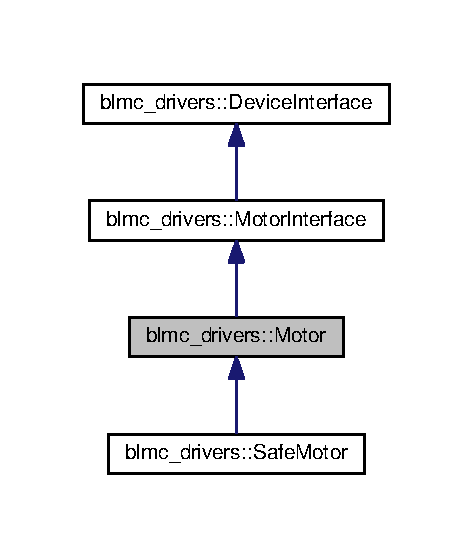
\includegraphics[width=227pt]{classblmc__drivers_1_1Motor__inherit__graph}
\end{center}
\end{figure}


Collaboration diagram for blmc\+\_\+drivers\+:\+:Motor\+:
\nopagebreak
\begin{figure}[H]
\begin{center}
\leavevmode
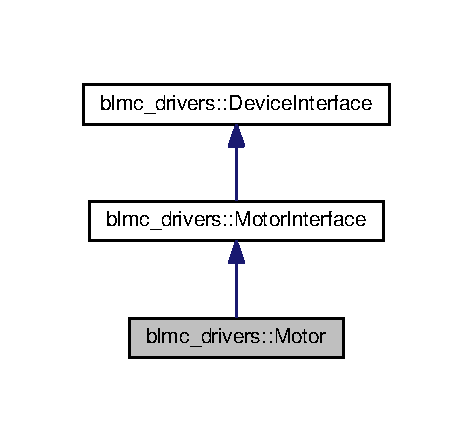
\includegraphics[width=227pt]{classblmc__drivers_1_1Motor__coll__graph}
\end{center}
\end{figure}
\subsection*{Public Member Functions}
\begin{DoxyCompactItemize}
\item 
\hyperlink{classblmc__drivers_1_1Motor_a923be3c8e5027cdead1006f3878b6ec3}{Motor} (\hyperlink{classblmc__drivers_1_1MotorInterface_ae31f230b9da3674a05543023c90b124c}{Ptr}$<$ \hyperlink{classblmc__drivers_1_1MotorBoardInterface}{Motor\+Board\+Interface} $>$ board, bool motor\+\_\+id)
\begin{DoxyCompactList}\small\item\em Construct a new \hyperlink{classblmc__drivers_1_1Motor}{Motor} object. \end{DoxyCompactList}\item 
virtual \hyperlink{classblmc__drivers_1_1Motor_ad93b64d54b40ff12df7081e009c71239}{$\sim$\+Motor} ()
\begin{DoxyCompactList}\small\item\em Destroy the \hyperlink{classblmc__drivers_1_1Motor}{Motor} object. \end{DoxyCompactList}\item 
virtual void \hyperlink{classblmc__drivers_1_1Motor_acf7389e09918c1955986a641efd4f032}{send\+\_\+if\+\_\+input\+\_\+changed} ()\hypertarget{classblmc__drivers_1_1Motor_acf7389e09918c1955986a641efd4f032}{}\label{classblmc__drivers_1_1Motor_acf7389e09918c1955986a641efd4f032}

\begin{DoxyCompactList}\small\item\em Actually send the command and controls via the network, See \hyperlink{classblmc__drivers_1_1MotorInterface}{Motor\+Interface} for more information. \end{DoxyCompactList}\item 
virtual \hyperlink{classblmc__drivers_1_1MotorInterface_ae31f230b9da3674a05543023c90b124c}{Ptr}$<$ const \hyperlink{classblmc__drivers_1_1MotorInterface_a49b8fc916b9f9debbd7b0988463db5cd}{Scalar\+Timeseries} $>$ \hyperlink{classblmc__drivers_1_1Motor_a919cb2f48cfc8550fabd5d3c5d7d0cf0}{get\+\_\+measurement} (const int \&index=0) const 
\begin{DoxyCompactList}\small\item\em Getters. \end{DoxyCompactList}\item 
virtual \hyperlink{classblmc__drivers_1_1MotorInterface_ae31f230b9da3674a05543023c90b124c}{Ptr}$<$ const \hyperlink{classblmc__drivers_1_1MotorInterface_a49b8fc916b9f9debbd7b0988463db5cd}{Scalar\+Timeseries} $>$ \hyperlink{classblmc__drivers_1_1Motor_ac1c0c4f1faa125bc0b245fdbe2590575}{get\+\_\+current\+\_\+target} () const 
\begin{DoxyCompactList}\small\item\em Get the current target to be sent. \end{DoxyCompactList}\item 
virtual \hyperlink{classblmc__drivers_1_1MotorInterface_ae31f230b9da3674a05543023c90b124c}{Ptr}$<$ const \hyperlink{classblmc__drivers_1_1MotorInterface_a49b8fc916b9f9debbd7b0988463db5cd}{Scalar\+Timeseries} $>$ \hyperlink{classblmc__drivers_1_1Motor_aa629114982c99453b4563a0ec06b9eea}{get\+\_\+sent\+\_\+current\+\_\+target} () const 
\begin{DoxyCompactList}\small\item\em Get the already sent current target values. \end{DoxyCompactList}\item 
virtual void \hyperlink{classblmc__drivers_1_1Motor_a48801c9858a7b1784b0a0ac4272fdaf5}{set\+\_\+current\+\_\+target} (const double \&current\+\_\+target)
\begin{DoxyCompactList}\small\item\em Setters. \end{DoxyCompactList}\item 
virtual void \hyperlink{classblmc__drivers_1_1Motor_a4af56df5466d011fc2a567dd815a6c1b}{set\+\_\+command} (const \hyperlink{classblmc__drivers_1_1MotorBoardCommand}{Motor\+Board\+Command} \&command)
\begin{DoxyCompactList}\small\item\em Set the command. \end{DoxyCompactList}\item 
virtual void \hyperlink{classblmc__drivers_1_1Motor_a26d75604f92c85ba127d690d0b7fdd59}{print} () const 
\begin{DoxyCompactList}\small\item\em Print the motor status and state. \end{DoxyCompactList}\end{DoxyCompactItemize}
\subsection*{Protected Attributes}
\begin{DoxyCompactItemize}
\item 
\hyperlink{classblmc__drivers_1_1MotorInterface_ae31f230b9da3674a05543023c90b124c}{Ptr}$<$ \hyperlink{classblmc__drivers_1_1MotorBoardInterface}{Motor\+Board\+Interface} $>$ \hyperlink{classblmc__drivers_1_1Motor_a779365c022edb7d4beb4060dcdb7dd72}{board\+\_\+}\hypertarget{classblmc__drivers_1_1Motor_a779365c022edb7d4beb4060dcdb7dd72}{}\label{classblmc__drivers_1_1Motor_a779365c022edb7d4beb4060dcdb7dd72}

\begin{DoxyCompactList}\small\item\em The Motor\+Board to be used for the communication. \end{DoxyCompactList}\item 
bool \hyperlink{classblmc__drivers_1_1Motor_a614903579bd6001169d11b72bc17042b}{motor\+\_\+id\+\_\+}\hypertarget{classblmc__drivers_1_1Motor_a614903579bd6001169d11b72bc17042b}{}\label{classblmc__drivers_1_1Motor_a614903579bd6001169d11b72bc17042b}

\begin{DoxyCompactList}\small\item\em The id of the motor on the Motor\+Board. \end{DoxyCompactList}\end{DoxyCompactItemize}
\subsection*{Additional Inherited Members}


\subsection{Detailed Description}
This class implements the \hyperlink{classblmc__drivers_1_1MotorInterface}{Motor\+Interface}. 

\subsection{Constructor \& Destructor Documentation}
\index{blmc\+\_\+drivers\+::\+Motor@{blmc\+\_\+drivers\+::\+Motor}!Motor@{Motor}}
\index{Motor@{Motor}!blmc\+\_\+drivers\+::\+Motor@{blmc\+\_\+drivers\+::\+Motor}}
\subsubsection[{\texorpdfstring{Motor(\+Ptr$<$ Motor\+Board\+Interface $>$ board, bool motor\+\_\+id)}{Motor(Ptr< MotorBoardInterface > board, bool motor_id)}}]{\setlength{\rightskip}{0pt plus 5cm}blmc\+\_\+drivers\+::\+Motor\+::\+Motor (
\begin{DoxyParamCaption}
\item[{{\bf Ptr}$<$ {\bf Motor\+Board\+Interface} $>$}]{board, }
\item[{bool}]{motor\+\_\+id}
\end{DoxyParamCaption}
)}\hypertarget{classblmc__drivers_1_1Motor_a923be3c8e5027cdead1006f3878b6ec3}{}\label{classblmc__drivers_1_1Motor_a923be3c8e5027cdead1006f3878b6ec3}


Construct a new \hyperlink{classblmc__drivers_1_1Motor}{Motor} object. 


\begin{DoxyParams}{Parameters}
{\em board} & is the Motor\+Board to be used. \\
\hline
{\em motor\+\_\+id} & is the id of the motor on the on-\/board card \\
\hline
\end{DoxyParams}
\index{blmc\+\_\+drivers\+::\+Motor@{blmc\+\_\+drivers\+::\+Motor}!````~Motor@{$\sim$\+Motor}}
\index{````~Motor@{$\sim$\+Motor}!blmc\+\_\+drivers\+::\+Motor@{blmc\+\_\+drivers\+::\+Motor}}
\subsubsection[{\texorpdfstring{$\sim$\+Motor()}{~Motor()}}]{\setlength{\rightskip}{0pt plus 5cm}virtual blmc\+\_\+drivers\+::\+Motor\+::$\sim$\+Motor (
\begin{DoxyParamCaption}
{}
\end{DoxyParamCaption}
)\hspace{0.3cm}{\ttfamily [inline]}, {\ttfamily [virtual]}}\hypertarget{classblmc__drivers_1_1Motor_ad93b64d54b40ff12df7081e009c71239}{}\label{classblmc__drivers_1_1Motor_ad93b64d54b40ff12df7081e009c71239}


Destroy the \hyperlink{classblmc__drivers_1_1Motor}{Motor} object. 



\subsection{Member Function Documentation}
\index{blmc\+\_\+drivers\+::\+Motor@{blmc\+\_\+drivers\+::\+Motor}!get\+\_\+current\+\_\+target@{get\+\_\+current\+\_\+target}}
\index{get\+\_\+current\+\_\+target@{get\+\_\+current\+\_\+target}!blmc\+\_\+drivers\+::\+Motor@{blmc\+\_\+drivers\+::\+Motor}}
\subsubsection[{\texorpdfstring{get\+\_\+current\+\_\+target() const }{get_current_target() const }}]{\setlength{\rightskip}{0pt plus 5cm}{\bf Motor\+::\+Ptr}$<$ const {\bf Motor\+::\+Scalar\+Timeseries} $>$ blmc\+\_\+drivers\+::\+Motor\+::get\+\_\+current\+\_\+target (
\begin{DoxyParamCaption}
{}
\end{DoxyParamCaption}
) const\hspace{0.3cm}{\ttfamily [virtual]}}\hypertarget{classblmc__drivers_1_1Motor_ac1c0c4f1faa125bc0b245fdbe2590575}{}\label{classblmc__drivers_1_1Motor_ac1c0c4f1faa125bc0b245fdbe2590575}


Get the current target to be sent. 

\begin{DoxyReturn}{Returns}
Ptr$<$const Scalar\+Timeseries$>$ the list of current values to be sent. 
\end{DoxyReturn}


Implements \hyperlink{classblmc__drivers_1_1MotorInterface_a167ffe5df0412b9abcac9a93861e58d2}{blmc\+\_\+drivers\+::\+Motor\+Interface}.



Reimplemented in \hyperlink{classblmc__drivers_1_1SafeMotor_a2c938b6289e41a7d3ab8a19a045382e0}{blmc\+\_\+drivers\+::\+Safe\+Motor}.

\index{blmc\+\_\+drivers\+::\+Motor@{blmc\+\_\+drivers\+::\+Motor}!get\+\_\+measurement@{get\+\_\+measurement}}
\index{get\+\_\+measurement@{get\+\_\+measurement}!blmc\+\_\+drivers\+::\+Motor@{blmc\+\_\+drivers\+::\+Motor}}
\subsubsection[{\texorpdfstring{get\+\_\+measurement(const int \&index=0) const }{get_measurement(const int &index=0) const }}]{\setlength{\rightskip}{0pt plus 5cm}{\bf Motor\+::\+Ptr}$<$ const {\bf Motor\+::\+Scalar\+Timeseries} $>$ blmc\+\_\+drivers\+::\+Motor\+::get\+\_\+measurement (
\begin{DoxyParamCaption}
\item[{const int \&}]{index = {\ttfamily 0}}
\end{DoxyParamCaption}
) const\hspace{0.3cm}{\ttfamily [virtual]}}\hypertarget{classblmc__drivers_1_1Motor_a919cb2f48cfc8550fabd5d3c5d7d0cf0}{}\label{classblmc__drivers_1_1Motor_a919cb2f48cfc8550fabd5d3c5d7d0cf0}


Getters. 

Get the measurements


\begin{DoxyParams}{Parameters}
{\em index} & is the kind of measurement we are instersted in. see \hyperlink{classblmc__drivers_1_1MotorInterface_a35c1217dd295078c67bacc2cba08ab33}{Motor\+Interface\+::\+Measurement\+Index}. \\
\hline
\end{DoxyParams}
\begin{DoxyReturn}{Returns}
Ptr$<$const Scalar\+Timeseries$>$ The history of the measurement 
\end{DoxyReturn}


Implements \hyperlink{classblmc__drivers_1_1MotorInterface_a7f6afed670f078518ccb46e1e3b44892}{blmc\+\_\+drivers\+::\+Motor\+Interface}.

\index{blmc\+\_\+drivers\+::\+Motor@{blmc\+\_\+drivers\+::\+Motor}!get\+\_\+sent\+\_\+current\+\_\+target@{get\+\_\+sent\+\_\+current\+\_\+target}}
\index{get\+\_\+sent\+\_\+current\+\_\+target@{get\+\_\+sent\+\_\+current\+\_\+target}!blmc\+\_\+drivers\+::\+Motor@{blmc\+\_\+drivers\+::\+Motor}}
\subsubsection[{\texorpdfstring{get\+\_\+sent\+\_\+current\+\_\+target() const }{get_sent_current_target() const }}]{\setlength{\rightskip}{0pt plus 5cm}{\bf Motor\+::\+Ptr}$<$ const {\bf Motor\+::\+Scalar\+Timeseries} $>$ blmc\+\_\+drivers\+::\+Motor\+::get\+\_\+sent\+\_\+current\+\_\+target (
\begin{DoxyParamCaption}
{}
\end{DoxyParamCaption}
) const\hspace{0.3cm}{\ttfamily [virtual]}}\hypertarget{classblmc__drivers_1_1Motor_aa629114982c99453b4563a0ec06b9eea}{}\label{classblmc__drivers_1_1Motor_aa629114982c99453b4563a0ec06b9eea}


Get the already sent current target values. 

\begin{DoxyReturn}{Returns}
Ptr$<$const Scalar\+Timeseries$>$ 
\end{DoxyReturn}


Implements \hyperlink{classblmc__drivers_1_1MotorInterface_a709804e11aa22fbb3107e781c9799bdb}{blmc\+\_\+drivers\+::\+Motor\+Interface}.

\index{blmc\+\_\+drivers\+::\+Motor@{blmc\+\_\+drivers\+::\+Motor}!print@{print}}
\index{print@{print}!blmc\+\_\+drivers\+::\+Motor@{blmc\+\_\+drivers\+::\+Motor}}
\subsubsection[{\texorpdfstring{print() const }{print() const }}]{\setlength{\rightskip}{0pt plus 5cm}void blmc\+\_\+drivers\+::\+Motor\+::print (
\begin{DoxyParamCaption}
{}
\end{DoxyParamCaption}
) const\hspace{0.3cm}{\ttfamily [virtual]}}\hypertarget{classblmc__drivers_1_1Motor_a26d75604f92c85ba127d690d0b7fdd59}{}\label{classblmc__drivers_1_1Motor_a26d75604f92c85ba127d690d0b7fdd59}


Print the motor status and state. 

\index{blmc\+\_\+drivers\+::\+Motor@{blmc\+\_\+drivers\+::\+Motor}!set\+\_\+command@{set\+\_\+command}}
\index{set\+\_\+command@{set\+\_\+command}!blmc\+\_\+drivers\+::\+Motor@{blmc\+\_\+drivers\+::\+Motor}}
\subsubsection[{\texorpdfstring{set\+\_\+command(const Motor\+Board\+Command \&command)}{set_command(const MotorBoardCommand &command)}}]{\setlength{\rightskip}{0pt plus 5cm}virtual void blmc\+\_\+drivers\+::\+Motor\+::set\+\_\+command (
\begin{DoxyParamCaption}
\item[{const {\bf Motor\+Board\+Command} \&}]{command}
\end{DoxyParamCaption}
)\hspace{0.3cm}{\ttfamily [inline]}, {\ttfamily [virtual]}}\hypertarget{classblmc__drivers_1_1Motor_a4af56df5466d011fc2a567dd815a6c1b}{}\label{classblmc__drivers_1_1Motor_a4af56df5466d011fc2a567dd815a6c1b}


Set the command. 

See \hyperlink{classblmc__drivers_1_1MotorInterface}{Motor\+Interface} for more information.


\begin{DoxyParams}{Parameters}
{\em command} & \\
\hline
\end{DoxyParams}


Implements \hyperlink{classblmc__drivers_1_1MotorInterface_a723a772b2be5beb0f07097a5b3e00a89}{blmc\+\_\+drivers\+::\+Motor\+Interface}.

\index{blmc\+\_\+drivers\+::\+Motor@{blmc\+\_\+drivers\+::\+Motor}!set\+\_\+current\+\_\+target@{set\+\_\+current\+\_\+target}}
\index{set\+\_\+current\+\_\+target@{set\+\_\+current\+\_\+target}!blmc\+\_\+drivers\+::\+Motor@{blmc\+\_\+drivers\+::\+Motor}}
\subsubsection[{\texorpdfstring{set\+\_\+current\+\_\+target(const double \&current\+\_\+target)}{set_current_target(const double &current_target)}}]{\setlength{\rightskip}{0pt plus 5cm}void blmc\+\_\+drivers\+::\+Motor\+::set\+\_\+current\+\_\+target (
\begin{DoxyParamCaption}
\item[{const double \&}]{current\+\_\+target}
\end{DoxyParamCaption}
)\hspace{0.3cm}{\ttfamily [virtual]}}\hypertarget{classblmc__drivers_1_1Motor_a48801c9858a7b1784b0a0ac4272fdaf5}{}\label{classblmc__drivers_1_1Motor_a48801c9858a7b1784b0a0ac4272fdaf5}


Setters. 

Set the current (Ampere) target. See \hyperlink{classblmc__drivers_1_1MotorInterface}{Motor\+Interface} for more information.


\begin{DoxyParams}{Parameters}
{\em current\+\_\+target} & in Ampere \\
\hline
\end{DoxyParams}


Implements \hyperlink{classblmc__drivers_1_1MotorInterface_a76b49a1228ad549fa407a54c8da14d13}{blmc\+\_\+drivers\+::\+Motor\+Interface}.



Reimplemented in \hyperlink{classblmc__drivers_1_1SafeMotor_adedaee24408b94b3d1ed8f856e218b12}{blmc\+\_\+drivers\+::\+Safe\+Motor}.



The documentation for this class was generated from the following files\+:\begin{DoxyCompactItemize}
\item 
include/blmc\+\_\+drivers/devices/\hyperlink{motor_8hpp}{motor.\+hpp}\item 
src/\hyperlink{motor_8cpp}{motor.\+cpp}\end{DoxyCompactItemize}

\hypertarget{classblmc__drivers_1_1MotorBoardCommand}{}\section{blmc\+\_\+drivers\+:\+:Motor\+Board\+Command Class Reference}
\label{classblmc__drivers_1_1MotorBoardCommand}\index{blmc\+\_\+drivers\+::\+Motor\+Board\+Command@{blmc\+\_\+drivers\+::\+Motor\+Board\+Command}}


This \hyperlink{classblmc__drivers_1_1MotorBoardCommand}{Motor\+Board\+Command} class is a data structurs that defines a command.  




{\ttfamily \#include $<$motor\+\_\+board.\+hpp$>$}

\subsection*{Public Types}
\begin{DoxyCompactItemize}
\item 
enum \hyperlink{classblmc__drivers_1_1MotorBoardCommand_abdbd6eb70164938ea91ae02000ccf7b2}{I\+Ds} \{ \\*
{\bfseries E\+N\+A\+B\+L\+E\+\_\+\+S\+YS} = 1, 
{\bfseries E\+N\+A\+B\+L\+E\+\_\+\+M\+T\+R1} = 2, 
{\bfseries E\+N\+A\+B\+L\+E\+\_\+\+M\+T\+R2} = 3, 
{\bfseries E\+N\+A\+B\+L\+E\+\_\+\+V\+S\+P\+R\+I\+N\+G1} = 4, 
\\*
{\bfseries E\+N\+A\+B\+L\+E\+\_\+\+V\+S\+P\+R\+I\+N\+G2} = 5, 
{\bfseries S\+E\+N\+D\+\_\+\+C\+U\+R\+R\+E\+NT} = 12, 
{\bfseries S\+E\+N\+D\+\_\+\+P\+O\+S\+I\+T\+I\+ON} = 13, 
{\bfseries S\+E\+N\+D\+\_\+\+V\+E\+L\+O\+C\+I\+TY} = 14, 
\\*
{\bfseries S\+E\+N\+D\+\_\+\+A\+D\+C6} = 15, 
{\bfseries S\+E\+N\+D\+\_\+\+E\+N\+C\+\_\+\+I\+N\+D\+EX} = 16, 
{\bfseries S\+E\+N\+D\+\_\+\+A\+LL} = 20, 
{\bfseries S\+E\+T\+\_\+\+C\+A\+N\+\_\+\+R\+E\+C\+V\+\_\+\+T\+I\+M\+E\+O\+UT} = 30, 
\\*
{\bfseries E\+N\+A\+B\+L\+E\+\_\+\+P\+O\+S\+\_\+\+R\+O\+L\+L\+O\+V\+E\+R\+\_\+\+E\+R\+R\+OR} = 31
 \}\hypertarget{classblmc__drivers_1_1MotorBoardCommand_abdbd6eb70164938ea91ae02000ccf7b2}{}\label{classblmc__drivers_1_1MotorBoardCommand_abdbd6eb70164938ea91ae02000ccf7b2}
\begin{DoxyCompactList}\small\item\em I\+Ds are the different implemented commands that one can send to the Motor\+Board. \end{DoxyCompactList}
\item 
enum \hyperlink{classblmc__drivers_1_1MotorBoardCommand_ad61acf8dcb8f6fcb382fc5cbc1e44615}{Contents} \{ {\bfseries E\+N\+A\+B\+LE} = 1, 
{\bfseries D\+I\+S\+A\+B\+LE} = 0
 \}\hypertarget{classblmc__drivers_1_1MotorBoardCommand_ad61acf8dcb8f6fcb382fc5cbc1e44615}{}\label{classblmc__drivers_1_1MotorBoardCommand_ad61acf8dcb8f6fcb382fc5cbc1e44615}
\begin{DoxyCompactList}\small\item\em Is the different command status. \end{DoxyCompactList}
\end{DoxyCompactItemize}
\subsection*{Public Member Functions}
\begin{DoxyCompactItemize}
\item 
\hyperlink{classblmc__drivers_1_1MotorBoardCommand_ad5ac32071cbf2854135fee7bb89acf4e}{Motor\+Board\+Command} ()\hypertarget{classblmc__drivers_1_1MotorBoardCommand_ad5ac32071cbf2854135fee7bb89acf4e}{}\label{classblmc__drivers_1_1MotorBoardCommand_ad5ac32071cbf2854135fee7bb89acf4e}

\begin{DoxyCompactList}\small\item\em Construct a new \hyperlink{classblmc__drivers_1_1MotorBoardCommand}{Motor\+Board\+Command} object. \end{DoxyCompactList}\item 
\hyperlink{classblmc__drivers_1_1MotorBoardCommand_ae7cf695d2600d84929729befc3cb29f9}{Motor\+Board\+Command} (uint32\+\_\+t id, int32\+\_\+t content)
\begin{DoxyCompactList}\small\item\em Construct a new \hyperlink{classblmc__drivers_1_1MotorBoardCommand}{Motor\+Board\+Command} object. \end{DoxyCompactList}\item 
void \hyperlink{classblmc__drivers_1_1MotorBoardCommand_aa8a54ff3faa6c2b4ce50c13a0d83bcb3}{print} () const \hypertarget{classblmc__drivers_1_1MotorBoardCommand_aa8a54ff3faa6c2b4ce50c13a0d83bcb3}{}\label{classblmc__drivers_1_1MotorBoardCommand_aa8a54ff3faa6c2b4ce50c13a0d83bcb3}

\begin{DoxyCompactList}\small\item\em Display on a terminal the status of the message. \end{DoxyCompactList}\end{DoxyCompactItemize}
\subsection*{Public Attributes}
\begin{DoxyCompactItemize}
\item 
uint32\+\_\+t \hyperlink{classblmc__drivers_1_1MotorBoardCommand_a31bfcc3cb1b2c35cbd5349123d884af4}{id\+\_\+}\hypertarget{classblmc__drivers_1_1MotorBoardCommand_a31bfcc3cb1b2c35cbd5349123d884af4}{}\label{classblmc__drivers_1_1MotorBoardCommand_a31bfcc3cb1b2c35cbd5349123d884af4}

\begin{DoxyCompactList}\small\item\em id\+\_\+ is the command to be modifies on the card. \end{DoxyCompactList}\item 
int32\+\_\+t \hyperlink{classblmc__drivers_1_1MotorBoardCommand_ac417b63a8cc8801a6757f4dce3b0810c}{content\+\_\+}\hypertarget{classblmc__drivers_1_1MotorBoardCommand_ac417b63a8cc8801a6757f4dce3b0810c}{}\label{classblmc__drivers_1_1MotorBoardCommand_ac417b63a8cc8801a6757f4dce3b0810c}

\begin{DoxyCompactList}\small\item\em content\+\_\+ is the value of teh command to be sent to the cards. \end{DoxyCompactList}\end{DoxyCompactItemize}


\subsection{Detailed Description}
This \hyperlink{classblmc__drivers_1_1MotorBoardCommand}{Motor\+Board\+Command} class is a data structurs that defines a command. 

\subsection{Constructor \& Destructor Documentation}
\index{blmc\+\_\+drivers\+::\+Motor\+Board\+Command@{blmc\+\_\+drivers\+::\+Motor\+Board\+Command}!Motor\+Board\+Command@{Motor\+Board\+Command}}
\index{Motor\+Board\+Command@{Motor\+Board\+Command}!blmc\+\_\+drivers\+::\+Motor\+Board\+Command@{blmc\+\_\+drivers\+::\+Motor\+Board\+Command}}
\subsubsection[{\texorpdfstring{Motor\+Board\+Command(uint32\+\_\+t id, int32\+\_\+t content)}{MotorBoardCommand(uint32_t id, int32_t content)}}]{\setlength{\rightskip}{0pt plus 5cm}blmc\+\_\+drivers\+::\+Motor\+Board\+Command\+::\+Motor\+Board\+Command (
\begin{DoxyParamCaption}
\item[{uint32\+\_\+t}]{id, }
\item[{int32\+\_\+t}]{content}
\end{DoxyParamCaption}
)\hspace{0.3cm}{\ttfamily [inline]}}\hypertarget{classblmc__drivers_1_1MotorBoardCommand_ae7cf695d2600d84929729befc3cb29f9}{}\label{classblmc__drivers_1_1MotorBoardCommand_ae7cf695d2600d84929729befc3cb29f9}


Construct a new \hyperlink{classblmc__drivers_1_1MotorBoardCommand}{Motor\+Board\+Command} object. 


\begin{DoxyParams}{Parameters}
{\em id} & defines the command to apply. \\
\hline
{\em content} & defines of the command is enabled or disabled. \\
\hline
\end{DoxyParams}


The documentation for this class was generated from the following file\+:\begin{DoxyCompactItemize}
\item 
include/blmc\+\_\+drivers/devices/\hyperlink{motor__board_8hpp}{motor\+\_\+board.\+hpp}\end{DoxyCompactItemize}

\hypertarget{classblmc__drivers_1_1MotorBoardInterface}{}\section{blmc\+\_\+drivers\+:\+:Motor\+Board\+Interface Class Reference}
\label{classblmc__drivers_1_1MotorBoardInterface}\index{blmc\+\_\+drivers\+::\+Motor\+Board\+Interface@{blmc\+\_\+drivers\+::\+Motor\+Board\+Interface}}


\hyperlink{classblmc__drivers_1_1MotorBoardInterface}{Motor\+Board\+Interface} declares an A\+PI to inacte with a Motor\+Board.  




{\ttfamily \#include $<$motor\+\_\+board.\+hpp$>$}



Inheritance diagram for blmc\+\_\+drivers\+:\+:Motor\+Board\+Interface\+:
\nopagebreak
\begin{figure}[H]
\begin{center}
\leavevmode
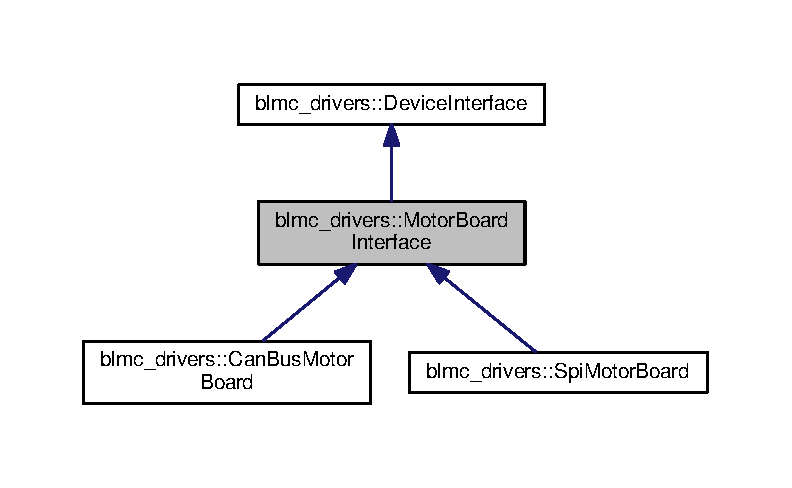
\includegraphics[width=350pt]{classblmc__drivers_1_1MotorBoardInterface__inherit__graph}
\end{center}
\end{figure}


Collaboration diagram for blmc\+\_\+drivers\+:\+:Motor\+Board\+Interface\+:
\nopagebreak
\begin{figure}[H]
\begin{center}
\leavevmode
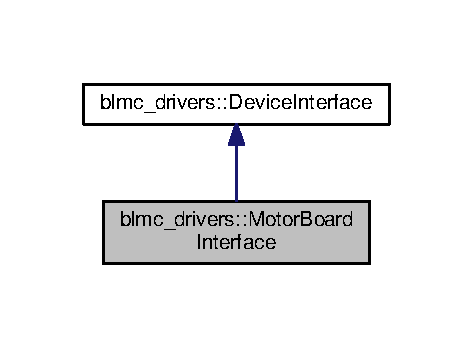
\includegraphics[width=227pt]{classblmc__drivers_1_1MotorBoardInterface__coll__graph}
\end{center}
\end{figure}
\subsection*{Public Types}
\begin{DoxyCompactItemize}
\item 
enum \hyperlink{classblmc__drivers_1_1MotorBoardInterface_a8e869cbdb9fcc872ba5a33813e0dfafb}{Measurement\+Index} \{ \\*
{\bfseries current\+\_\+0}, 
{\bfseries current\+\_\+1}, 
{\bfseries position\+\_\+0}, 
{\bfseries position\+\_\+1}, 
\\*
{\bfseries velocity\+\_\+0}, 
{\bfseries velocity\+\_\+1}, 
{\bfseries analog\+\_\+0}, 
{\bfseries analog\+\_\+1}, 
\\*
{\bfseries encoder\+\_\+index\+\_\+0}, 
{\bfseries encoder\+\_\+index\+\_\+1}, 
{\bfseries measurement\+\_\+count}
 \}\hypertarget{classblmc__drivers_1_1MotorBoardInterface_a8e869cbdb9fcc872ba5a33813e0dfafb}{}\label{classblmc__drivers_1_1MotorBoardInterface_a8e869cbdb9fcc872ba5a33813e0dfafb}
\begin{DoxyCompactList}\small\item\em This is the list of the measurement we can access. \end{DoxyCompactList}
\item 
enum \hyperlink{classblmc__drivers_1_1MotorBoardInterface_a82ed4d0fa527521707281396095a88ca}{Control\+Index} \{ {\bfseries current\+\_\+target\+\_\+0}, 
{\bfseries current\+\_\+target\+\_\+1}, 
{\bfseries control\+\_\+count}
 \}\hypertarget{classblmc__drivers_1_1MotorBoardInterface_a82ed4d0fa527521707281396095a88ca}{}\label{classblmc__drivers_1_1MotorBoardInterface_a82ed4d0fa527521707281396095a88ca}
\begin{DoxyCompactList}\small\item\em This is the list of the controls we can send. \end{DoxyCompactList}
\item 
typedef real\+\_\+time\+\_\+tools\+::\+Threadsafe\+Timeseries$<$ double $>$ \hyperlink{classblmc__drivers_1_1MotorBoardInterface_a14e237254ba495a66091ea3a3a33fa75}{Scalar\+Timeseries}\hypertarget{classblmc__drivers_1_1MotorBoardInterface_a14e237254ba495a66091ea3a3a33fa75}{}\label{classblmc__drivers_1_1MotorBoardInterface_a14e237254ba495a66091ea3a3a33fa75}

\begin{DoxyCompactList}\small\item\em A useful shortcut. \end{DoxyCompactList}\item 
typedef Scalar\+Timeseries\+::\+Index \hyperlink{classblmc__drivers_1_1MotorBoardInterface_ab0e201396fe808cbc480b69768c81fa2}{Index}\hypertarget{classblmc__drivers_1_1MotorBoardInterface_ab0e201396fe808cbc480b69768c81fa2}{}\label{classblmc__drivers_1_1MotorBoardInterface_ab0e201396fe808cbc480b69768c81fa2}

\begin{DoxyCompactList}\small\item\em A useful shortcut. \end{DoxyCompactList}\item 
typedef real\+\_\+time\+\_\+tools\+::\+Threadsafe\+Timeseries$<$ \hyperlink{classblmc__drivers_1_1MotorBoardInterface_ab0e201396fe808cbc480b69768c81fa2}{Index} $>$ \hyperlink{classblmc__drivers_1_1MotorBoardInterface_aef0ca990410b130b67abce74d20d58a5}{Index\+Timeseries}\hypertarget{classblmc__drivers_1_1MotorBoardInterface_aef0ca990410b130b67abce74d20d58a5}{}\label{classblmc__drivers_1_1MotorBoardInterface_aef0ca990410b130b67abce74d20d58a5}

\begin{DoxyCompactList}\small\item\em A useful shortcut. \end{DoxyCompactList}\item 
typedef real\+\_\+time\+\_\+tools\+::\+Threadsafe\+Timeseries$<$ \hyperlink{classblmc__drivers_1_1MotorBoardStatus}{Motor\+Board\+Status} $>$ \hyperlink{classblmc__drivers_1_1MotorBoardInterface_ae3777e484dda60c4abe87f2b542ddfb8}{Status\+Timeseries}\hypertarget{classblmc__drivers_1_1MotorBoardInterface_ae3777e484dda60c4abe87f2b542ddfb8}{}\label{classblmc__drivers_1_1MotorBoardInterface_ae3777e484dda60c4abe87f2b542ddfb8}

\begin{DoxyCompactList}\small\item\em A useful shortcut. \end{DoxyCompactList}\item 
typedef real\+\_\+time\+\_\+tools\+::\+Threadsafe\+Timeseries$<$ \hyperlink{classblmc__drivers_1_1MotorBoardCommand}{Motor\+Board\+Command} $>$ \hyperlink{classblmc__drivers_1_1MotorBoardInterface_ae2afe94a023d9f08a4c689e9b7660f15}{Command\+Timeseries}\hypertarget{classblmc__drivers_1_1MotorBoardInterface_ae2afe94a023d9f08a4c689e9b7660f15}{}\label{classblmc__drivers_1_1MotorBoardInterface_ae2afe94a023d9f08a4c689e9b7660f15}

\begin{DoxyCompactList}\small\item\em A useful shortcut. \end{DoxyCompactList}\item 
{\footnotesize template$<$typename Type $>$ }\\using \hyperlink{classblmc__drivers_1_1MotorBoardInterface_a6a733b7ed7a3a96f6b0712b6bb5307f8}{Ptr} = std\+::shared\+\_\+ptr$<$ Type $>$\hypertarget{classblmc__drivers_1_1MotorBoardInterface_a6a733b7ed7a3a96f6b0712b6bb5307f8}{}\label{classblmc__drivers_1_1MotorBoardInterface_a6a733b7ed7a3a96f6b0712b6bb5307f8}

\begin{DoxyCompactList}\small\item\em A useful shortcut. \end{DoxyCompactList}\item 
{\footnotesize template$<$typename Type $>$ }\\using \hyperlink{classblmc__drivers_1_1MotorBoardInterface_abeb474bef6d85dffcd5227e5ea965cc5}{Vector} = std\+::vector$<$ Type $>$\hypertarget{classblmc__drivers_1_1MotorBoardInterface_abeb474bef6d85dffcd5227e5ea965cc5}{}\label{classblmc__drivers_1_1MotorBoardInterface_abeb474bef6d85dffcd5227e5ea965cc5}

\begin{DoxyCompactList}\small\item\em A useful shortcut. \end{DoxyCompactList}\end{DoxyCompactItemize}
\subsection*{Public Member Functions}
\begin{DoxyCompactItemize}
\item 
virtual \hyperlink{classblmc__drivers_1_1MotorBoardInterface_aecd23682c4a8c0df8e57b4c752e1d9ee}{$\sim$\+Motor\+Board\+Interface} ()\hypertarget{classblmc__drivers_1_1MotorBoardInterface_aecd23682c4a8c0df8e57b4c752e1d9ee}{}\label{classblmc__drivers_1_1MotorBoardInterface_aecd23682c4a8c0df8e57b4c752e1d9ee}

\begin{DoxyCompactList}\small\item\em Destroy the \hyperlink{classblmc__drivers_1_1MotorBoardInterface}{Motor\+Board\+Interface} object. \end{DoxyCompactList}\item 
virtual \hyperlink{classblmc__drivers_1_1MotorBoardInterface_a6a733b7ed7a3a96f6b0712b6bb5307f8}{Ptr}$<$ const \hyperlink{classblmc__drivers_1_1MotorBoardInterface_a14e237254ba495a66091ea3a3a33fa75}{Scalar\+Timeseries} $>$ \hyperlink{classblmc__drivers_1_1MotorBoardInterface_a34828a0375a3bd1fede4deb4fc74c04d}{get\+\_\+measurement} (const int \&index) const =0
\begin{DoxyCompactList}\small\item\em Getters. \end{DoxyCompactList}\item 
virtual \hyperlink{classblmc__drivers_1_1MotorBoardInterface_a6a733b7ed7a3a96f6b0712b6bb5307f8}{Ptr}$<$ const \hyperlink{classblmc__drivers_1_1MotorBoardInterface_ae3777e484dda60c4abe87f2b542ddfb8}{Status\+Timeseries} $>$ \hyperlink{classblmc__drivers_1_1MotorBoardInterface_a13b1ffa7d10c1c753d76eaf5368714e3}{get\+\_\+status} () const =0
\begin{DoxyCompactList}\small\item\em Get the status of the motor board. \end{DoxyCompactList}\item 
virtual \hyperlink{classblmc__drivers_1_1MotorBoardInterface_a6a733b7ed7a3a96f6b0712b6bb5307f8}{Ptr}$<$ const \hyperlink{classblmc__drivers_1_1MotorBoardInterface_a14e237254ba495a66091ea3a3a33fa75}{Scalar\+Timeseries} $>$ \hyperlink{classblmc__drivers_1_1MotorBoardInterface_aa5eeed12c851993f2e2c93f5479df9de}{get\+\_\+control} (const int \&index) const =0
\begin{DoxyCompactList}\small\item\em input logs \end{DoxyCompactList}\item 
virtual \hyperlink{classblmc__drivers_1_1MotorBoardInterface_a6a733b7ed7a3a96f6b0712b6bb5307f8}{Ptr}$<$ const \hyperlink{classblmc__drivers_1_1MotorBoardInterface_ae2afe94a023d9f08a4c689e9b7660f15}{Command\+Timeseries} $>$ \hyperlink{classblmc__drivers_1_1MotorBoardInterface_a4913308c1eacc98475aeb8647447c997}{get\+\_\+command} () const =0
\begin{DoxyCompactList}\small\item\em Get the commands to be send. \end{DoxyCompactList}\item 
virtual \hyperlink{classblmc__drivers_1_1MotorBoardInterface_a6a733b7ed7a3a96f6b0712b6bb5307f8}{Ptr}$<$ const \hyperlink{classblmc__drivers_1_1MotorBoardInterface_a14e237254ba495a66091ea3a3a33fa75}{Scalar\+Timeseries} $>$ \hyperlink{classblmc__drivers_1_1MotorBoardInterface_a8dc6222e915fc96d89b13cbb0fcb0cda}{get\+\_\+sent\+\_\+control} (const int \&index) const =0
\begin{DoxyCompactList}\small\item\em Get the sent controls. \end{DoxyCompactList}\item 
virtual \hyperlink{classblmc__drivers_1_1MotorBoardInterface_a6a733b7ed7a3a96f6b0712b6bb5307f8}{Ptr}$<$ const \hyperlink{classblmc__drivers_1_1MotorBoardInterface_ae2afe94a023d9f08a4c689e9b7660f15}{Command\+Timeseries} $>$ \hyperlink{classblmc__drivers_1_1MotorBoardInterface_afd3de58f7a900347154b8d323f1c1d94}{get\+\_\+sent\+\_\+command} () const =0
\begin{DoxyCompactList}\small\item\em Get the sent commands. \end{DoxyCompactList}\item 
virtual void \hyperlink{classblmc__drivers_1_1MotorBoardInterface_a3ace57ba3e09b9b3120d09303ff39a61}{set\+\_\+control} (const double \&control, const int \&index)=0
\begin{DoxyCompactList}\small\item\em Setters. \end{DoxyCompactList}\item 
virtual void \hyperlink{classblmc__drivers_1_1MotorBoardInterface_a86b4ff810ca652d6761090ceaff65621}{set\+\_\+command} (const \hyperlink{classblmc__drivers_1_1MotorBoardCommand}{Motor\+Board\+Command} \&command)=0
\begin{DoxyCompactList}\small\item\em set\+\_\+command save the command internally. \end{DoxyCompactList}\item 
virtual void \hyperlink{classblmc__drivers_1_1MotorBoardInterface_a79afd172c736718868f4d269125f2581}{send\+\_\+if\+\_\+input\+\_\+changed} ()=0\hypertarget{classblmc__drivers_1_1MotorBoardInterface_a79afd172c736718868f4d269125f2581}{}\label{classblmc__drivers_1_1MotorBoardInterface_a79afd172c736718868f4d269125f2581}

\begin{DoxyCompactList}\small\item\em Actually send the commands and the controls. \end{DoxyCompactList}\end{DoxyCompactItemize}


\subsection{Detailed Description}
\hyperlink{classblmc__drivers_1_1MotorBoardInterface}{Motor\+Board\+Interface} declares an A\+PI to inacte with a Motor\+Board. 

\subsection{Member Function Documentation}
\index{blmc\+\_\+drivers\+::\+Motor\+Board\+Interface@{blmc\+\_\+drivers\+::\+Motor\+Board\+Interface}!get\+\_\+command@{get\+\_\+command}}
\index{get\+\_\+command@{get\+\_\+command}!blmc\+\_\+drivers\+::\+Motor\+Board\+Interface@{blmc\+\_\+drivers\+::\+Motor\+Board\+Interface}}
\subsubsection[{\texorpdfstring{get\+\_\+command() const =0}{get_command() const =0}}]{\setlength{\rightskip}{0pt plus 5cm}virtual {\bf Ptr}$<$const {\bf Command\+Timeseries}$>$ blmc\+\_\+drivers\+::\+Motor\+Board\+Interface\+::get\+\_\+command (
\begin{DoxyParamCaption}
{}
\end{DoxyParamCaption}
) const\hspace{0.3cm}{\ttfamily [pure virtual]}}\hypertarget{classblmc__drivers_1_1MotorBoardInterface_a4913308c1eacc98475aeb8647447c997}{}\label{classblmc__drivers_1_1MotorBoardInterface_a4913308c1eacc98475aeb8647447c997}


Get the commands to be send. 

\begin{DoxyReturn}{Returns}
Ptr$<$const Command\+Timeseries$>$ is the list of the commands to be send. 
\end{DoxyReturn}


Implemented in \hyperlink{classblmc__drivers_1_1CanBusMotorBoard_abc8f5d6a631dc01a236d623754362e7d}{blmc\+\_\+drivers\+::\+Can\+Bus\+Motor\+Board}, and \hyperlink{classblmc__drivers_1_1SpiMotorBoard_a3a3b3b043762c2a232d7e724aea8a6ff}{blmc\+\_\+drivers\+::\+Spi\+Motor\+Board}.

\index{blmc\+\_\+drivers\+::\+Motor\+Board\+Interface@{blmc\+\_\+drivers\+::\+Motor\+Board\+Interface}!get\+\_\+control@{get\+\_\+control}}
\index{get\+\_\+control@{get\+\_\+control}!blmc\+\_\+drivers\+::\+Motor\+Board\+Interface@{blmc\+\_\+drivers\+::\+Motor\+Board\+Interface}}
\subsubsection[{\texorpdfstring{get\+\_\+control(const int \&index) const =0}{get_control(const int &index) const =0}}]{\setlength{\rightskip}{0pt plus 5cm}virtual {\bf Ptr}$<$const {\bf Scalar\+Timeseries}$>$ blmc\+\_\+drivers\+::\+Motor\+Board\+Interface\+::get\+\_\+control (
\begin{DoxyParamCaption}
\item[{const int \&}]{index}
\end{DoxyParamCaption}
) const\hspace{0.3cm}{\ttfamily [pure virtual]}}\hypertarget{classblmc__drivers_1_1MotorBoardInterface_aa5eeed12c851993f2e2c93f5479df9de}{}\label{classblmc__drivers_1_1MotorBoardInterface_aa5eeed12c851993f2e2c93f5479df9de}


input logs 

Get the controls to be send.


\begin{DoxyParams}{Parameters}
{\em index} & define the kind of control we are looking for. \\
\hline
\end{DoxyParams}
\begin{DoxyReturn}{Returns}
Ptr$<$const Scalar\+Timeseries$>$ is the list of the controls to be send. 
\end{DoxyReturn}


Implemented in \hyperlink{classblmc__drivers_1_1CanBusMotorBoard_a298403ab64585ed459eda57165057fef}{blmc\+\_\+drivers\+::\+Can\+Bus\+Motor\+Board}, and \hyperlink{classblmc__drivers_1_1SpiMotorBoard_a1b145982a241e234118269c7eeea8d42}{blmc\+\_\+drivers\+::\+Spi\+Motor\+Board}.

\index{blmc\+\_\+drivers\+::\+Motor\+Board\+Interface@{blmc\+\_\+drivers\+::\+Motor\+Board\+Interface}!get\+\_\+measurement@{get\+\_\+measurement}}
\index{get\+\_\+measurement@{get\+\_\+measurement}!blmc\+\_\+drivers\+::\+Motor\+Board\+Interface@{blmc\+\_\+drivers\+::\+Motor\+Board\+Interface}}
\subsubsection[{\texorpdfstring{get\+\_\+measurement(const int \&index) const =0}{get_measurement(const int &index) const =0}}]{\setlength{\rightskip}{0pt plus 5cm}virtual {\bf Ptr}$<$const {\bf Scalar\+Timeseries}$>$ blmc\+\_\+drivers\+::\+Motor\+Board\+Interface\+::get\+\_\+measurement (
\begin{DoxyParamCaption}
\item[{const int \&}]{index}
\end{DoxyParamCaption}
) const\hspace{0.3cm}{\ttfamily [pure virtual]}}\hypertarget{classblmc__drivers_1_1MotorBoardInterface_a34828a0375a3bd1fede4deb4fc74c04d}{}\label{classblmc__drivers_1_1MotorBoardInterface_a34828a0375a3bd1fede4deb4fc74c04d}


Getters. 

Get the measurements


\begin{DoxyParams}{Parameters}
{\em index} & is the kind of measurement we are looking for. \\
\hline
\end{DoxyParams}
\begin{DoxyReturn}{Returns}
Ptr$<$const Scalar\+Timeseries$>$ is the list of the last time stamped measurement acquiered. 
\end{DoxyReturn}


Implemented in \hyperlink{classblmc__drivers_1_1CanBusMotorBoard_a38094207eed00f6b1d75cfe9b5b87046}{blmc\+\_\+drivers\+::\+Can\+Bus\+Motor\+Board}, and \hyperlink{classblmc__drivers_1_1SpiMotorBoard_ae0979b63fe72f5717a156fe670df6b32}{blmc\+\_\+drivers\+::\+Spi\+Motor\+Board}.

\index{blmc\+\_\+drivers\+::\+Motor\+Board\+Interface@{blmc\+\_\+drivers\+::\+Motor\+Board\+Interface}!get\+\_\+sent\+\_\+command@{get\+\_\+sent\+\_\+command}}
\index{get\+\_\+sent\+\_\+command@{get\+\_\+sent\+\_\+command}!blmc\+\_\+drivers\+::\+Motor\+Board\+Interface@{blmc\+\_\+drivers\+::\+Motor\+Board\+Interface}}
\subsubsection[{\texorpdfstring{get\+\_\+sent\+\_\+command() const =0}{get_sent_command() const =0}}]{\setlength{\rightskip}{0pt plus 5cm}virtual {\bf Ptr}$<$const {\bf Command\+Timeseries}$>$ blmc\+\_\+drivers\+::\+Motor\+Board\+Interface\+::get\+\_\+sent\+\_\+command (
\begin{DoxyParamCaption}
{}
\end{DoxyParamCaption}
) const\hspace{0.3cm}{\ttfamily [pure virtual]}}\hypertarget{classblmc__drivers_1_1MotorBoardInterface_afd3de58f7a900347154b8d323f1c1d94}{}\label{classblmc__drivers_1_1MotorBoardInterface_afd3de58f7a900347154b8d323f1c1d94}


Get the sent commands. 

\begin{DoxyReturn}{Returns}
Ptr$<$const Command\+Timeseries$>$ is the list of the commands sent recently. 
\end{DoxyReturn}


Implemented in \hyperlink{classblmc__drivers_1_1CanBusMotorBoard_a4e2920571e42aafa8045d1148f078a3a}{blmc\+\_\+drivers\+::\+Can\+Bus\+Motor\+Board}, and \hyperlink{classblmc__drivers_1_1SpiMotorBoard_a187c15b804f4e7b49f2cd21625ae2512}{blmc\+\_\+drivers\+::\+Spi\+Motor\+Board}.

\index{blmc\+\_\+drivers\+::\+Motor\+Board\+Interface@{blmc\+\_\+drivers\+::\+Motor\+Board\+Interface}!get\+\_\+sent\+\_\+control@{get\+\_\+sent\+\_\+control}}
\index{get\+\_\+sent\+\_\+control@{get\+\_\+sent\+\_\+control}!blmc\+\_\+drivers\+::\+Motor\+Board\+Interface@{blmc\+\_\+drivers\+::\+Motor\+Board\+Interface}}
\subsubsection[{\texorpdfstring{get\+\_\+sent\+\_\+control(const int \&index) const =0}{get_sent_control(const int &index) const =0}}]{\setlength{\rightskip}{0pt plus 5cm}virtual {\bf Ptr}$<$const {\bf Scalar\+Timeseries}$>$ blmc\+\_\+drivers\+::\+Motor\+Board\+Interface\+::get\+\_\+sent\+\_\+control (
\begin{DoxyParamCaption}
\item[{const int \&}]{index}
\end{DoxyParamCaption}
) const\hspace{0.3cm}{\ttfamily [pure virtual]}}\hypertarget{classblmc__drivers_1_1MotorBoardInterface_a8dc6222e915fc96d89b13cbb0fcb0cda}{}\label{classblmc__drivers_1_1MotorBoardInterface_a8dc6222e915fc96d89b13cbb0fcb0cda}


Get the sent controls. 


\begin{DoxyParams}{Parameters}
{\em index} & define the kind of control we are looking for. \\
\hline
\end{DoxyParams}
\begin{DoxyReturn}{Returns}
Ptr$<$const Scalar\+Timeseries$>$ is the list of the controls sent recently. 
\end{DoxyReturn}


Implemented in \hyperlink{classblmc__drivers_1_1CanBusMotorBoard_a907629485fcf006e1e61b9739d3c94ec}{blmc\+\_\+drivers\+::\+Can\+Bus\+Motor\+Board}, and \hyperlink{classblmc__drivers_1_1SpiMotorBoard_a26b6e07529dfdbae891a61d6823e3bdb}{blmc\+\_\+drivers\+::\+Spi\+Motor\+Board}.

\index{blmc\+\_\+drivers\+::\+Motor\+Board\+Interface@{blmc\+\_\+drivers\+::\+Motor\+Board\+Interface}!get\+\_\+status@{get\+\_\+status}}
\index{get\+\_\+status@{get\+\_\+status}!blmc\+\_\+drivers\+::\+Motor\+Board\+Interface@{blmc\+\_\+drivers\+::\+Motor\+Board\+Interface}}
\subsubsection[{\texorpdfstring{get\+\_\+status() const =0}{get_status() const =0}}]{\setlength{\rightskip}{0pt plus 5cm}virtual {\bf Ptr}$<$const {\bf Status\+Timeseries}$>$ blmc\+\_\+drivers\+::\+Motor\+Board\+Interface\+::get\+\_\+status (
\begin{DoxyParamCaption}
{}
\end{DoxyParamCaption}
) const\hspace{0.3cm}{\ttfamily [pure virtual]}}\hypertarget{classblmc__drivers_1_1MotorBoardInterface_a13b1ffa7d10c1c753d76eaf5368714e3}{}\label{classblmc__drivers_1_1MotorBoardInterface_a13b1ffa7d10c1c753d76eaf5368714e3}


Get the status of the motor board. 

\begin{DoxyReturn}{Returns}
Ptr$<$const Status\+Timeseries$>$ is the list of the last status of the card. 
\end{DoxyReturn}


Implemented in \hyperlink{classblmc__drivers_1_1CanBusMotorBoard_a04aef38d8490ed8ac0e12cb09ef313e4}{blmc\+\_\+drivers\+::\+Can\+Bus\+Motor\+Board}, and \hyperlink{classblmc__drivers_1_1SpiMotorBoard_a74e1b0e71721f72769870b7c857f6d92}{blmc\+\_\+drivers\+::\+Spi\+Motor\+Board}.

\index{blmc\+\_\+drivers\+::\+Motor\+Board\+Interface@{blmc\+\_\+drivers\+::\+Motor\+Board\+Interface}!set\+\_\+command@{set\+\_\+command}}
\index{set\+\_\+command@{set\+\_\+command}!blmc\+\_\+drivers\+::\+Motor\+Board\+Interface@{blmc\+\_\+drivers\+::\+Motor\+Board\+Interface}}
\subsubsection[{\texorpdfstring{set\+\_\+command(const Motor\+Board\+Command \&command)=0}{set_command(const MotorBoardCommand &command)=0}}]{\setlength{\rightskip}{0pt plus 5cm}virtual void blmc\+\_\+drivers\+::\+Motor\+Board\+Interface\+::set\+\_\+command (
\begin{DoxyParamCaption}
\item[{const {\bf Motor\+Board\+Command} \&}]{command}
\end{DoxyParamCaption}
)\hspace{0.3cm}{\ttfamily [pure virtual]}}\hypertarget{classblmc__drivers_1_1MotorBoardInterface_a86b4ff810ca652d6761090ceaff65621}{}\label{classblmc__drivers_1_1MotorBoardInterface_a86b4ff810ca652d6761090ceaff65621}


set\+\_\+command save the command internally. 

In order to actaully send the controls to the network please call \char`\"{}send\+\_\+if\+\_\+input\+\_\+changed\char`\"{}


\begin{DoxyParams}{Parameters}
{\em command} & is the command to be sent. \\
\hline
\end{DoxyParams}


Implemented in \hyperlink{classblmc__drivers_1_1CanBusMotorBoard_a4bb9c1f7f59507feed145111ccffc625}{blmc\+\_\+drivers\+::\+Can\+Bus\+Motor\+Board}, and \hyperlink{classblmc__drivers_1_1SpiMotorBoard_a6b626225af993444bdee397952281772}{blmc\+\_\+drivers\+::\+Spi\+Motor\+Board}.

\index{blmc\+\_\+drivers\+::\+Motor\+Board\+Interface@{blmc\+\_\+drivers\+::\+Motor\+Board\+Interface}!set\+\_\+control@{set\+\_\+control}}
\index{set\+\_\+control@{set\+\_\+control}!blmc\+\_\+drivers\+::\+Motor\+Board\+Interface@{blmc\+\_\+drivers\+::\+Motor\+Board\+Interface}}
\subsubsection[{\texorpdfstring{set\+\_\+control(const double \&control, const int \&index)=0}{set_control(const double &control, const int &index)=0}}]{\setlength{\rightskip}{0pt plus 5cm}virtual void blmc\+\_\+drivers\+::\+Motor\+Board\+Interface\+::set\+\_\+control (
\begin{DoxyParamCaption}
\item[{const double \&}]{control, }
\item[{const int \&}]{index}
\end{DoxyParamCaption}
)\hspace{0.3cm}{\ttfamily [pure virtual]}}\hypertarget{classblmc__drivers_1_1MotorBoardInterface_a3ace57ba3e09b9b3120d09303ff39a61}{}\label{classblmc__drivers_1_1MotorBoardInterface_a3ace57ba3e09b9b3120d09303ff39a61}


Setters. 

set\+\_\+control save the control internally. In order to actaully send the controls to the network please call \char`\"{}send\+\_\+if\+\_\+input\+\_\+changed\char`\"{}


\begin{DoxyParams}{Parameters}
{\em control} & is the value of the control. \\
\hline
{\em index} & define the kind of control we want to send. \\
\hline
\end{DoxyParams}


Implemented in \hyperlink{classblmc__drivers_1_1CanBusMotorBoard_a8dbd787fcfc25d68d5443e2f0bf21f64}{blmc\+\_\+drivers\+::\+Can\+Bus\+Motor\+Board}, and \hyperlink{classblmc__drivers_1_1SpiMotorBoard_ae11c5382665adfa718bcc43ec1e84b6e}{blmc\+\_\+drivers\+::\+Spi\+Motor\+Board}.



The documentation for this class was generated from the following file\+:\begin{DoxyCompactItemize}
\item 
include/blmc\+\_\+drivers/devices/\hyperlink{motor__board_8hpp}{motor\+\_\+board.\+hpp}\end{DoxyCompactItemize}

\hypertarget{classblmc__drivers_1_1MotorBoardStatus}{}\section{blmc\+\_\+drivers\+:\+:Motor\+Board\+Status Class Reference}
\label{classblmc__drivers_1_1MotorBoardStatus}\index{blmc\+\_\+drivers\+::\+Motor\+Board\+Status@{blmc\+\_\+drivers\+::\+Motor\+Board\+Status}}


This class represent a 8 bits message that describe the state (enable/disabled) of the card and the two motors.  




{\ttfamily \#include $<$motor\+\_\+board.\+hpp$>$}

\subsection*{Public Types}
\begin{DoxyCompactItemize}
\item 
enum \hyperlink{classblmc__drivers_1_1MotorBoardStatus_a9fd931e24550f5e5877d7a6cf499f6cf}{Error\+Codes} \{ \\*
\hyperlink{classblmc__drivers_1_1MotorBoardStatus_a9fd931e24550f5e5877d7a6cf499f6cfa99d623b3894cfb91a0626b56d0583f84}{N\+O\+NE} = 0, 
\hyperlink{classblmc__drivers_1_1MotorBoardStatus_a9fd931e24550f5e5877d7a6cf499f6cfab3a0b4c22659f24593503e41fce561d0}{E\+N\+C\+O\+D\+ER} = 1, 
\hyperlink{classblmc__drivers_1_1MotorBoardStatus_a9fd931e24550f5e5877d7a6cf499f6cfa25dd0ce676d69449a6fe0a02fa6e6a5d}{C\+A\+N\+\_\+\+R\+E\+C\+V\+\_\+\+T\+I\+M\+E\+O\+UT} = 2, 
\hyperlink{classblmc__drivers_1_1MotorBoardStatus_a9fd931e24550f5e5877d7a6cf499f6cfa43b0778d39a1aa2c193e2b511f2fe511}{C\+R\+I\+T\+\_\+\+T\+E\+MP} = 3, 
\\*
\hyperlink{classblmc__drivers_1_1MotorBoardStatus_a9fd931e24550f5e5877d7a6cf499f6cfa3134cc4a15dfbbeccd1305ad7f0e56cf}{P\+O\+S\+C\+O\+NV} = 4, 
\hyperlink{classblmc__drivers_1_1MotorBoardStatus_a9fd931e24550f5e5877d7a6cf499f6cfa87717db1d2ce92549a0bd95890c45f63}{P\+O\+S\+\_\+\+R\+O\+L\+L\+O\+V\+ER} = 5, 
\hyperlink{classblmc__drivers_1_1MotorBoardStatus_a9fd931e24550f5e5877d7a6cf499f6cfa2b6b3fa06a4bf24105805b604aff7280}{O\+T\+H\+ER} = 7
 \}\begin{DoxyCompactList}\small\item\em This is the list of the error codes. \end{DoxyCompactList}
\end{DoxyCompactItemize}
\subsection*{Public Member Functions}
\begin{DoxyCompactItemize}
\item 
void \hyperlink{classblmc__drivers_1_1MotorBoardStatus_ac050ae0cdf1c6e56ebd241c41330a42d}{print} () const \hypertarget{classblmc__drivers_1_1MotorBoardStatus_ac050ae0cdf1c6e56ebd241c41330a42d}{}\label{classblmc__drivers_1_1MotorBoardStatus_ac050ae0cdf1c6e56ebd241c41330a42d}

\begin{DoxyCompactList}\small\item\em Simply print the status of the motor board. \end{DoxyCompactList}\item 
bool \hyperlink{classblmc__drivers_1_1MotorBoardStatus_a1da75ba70f6ad31fa7c880b5c673cc89}{is\+\_\+ready} ()
\begin{DoxyCompactList}\small\item\em Check if the all status are green. \end{DoxyCompactList}\end{DoxyCompactItemize}
\subsection*{Public Attributes}
\begin{DoxyCompactItemize}
\item 
uint8\+\_\+t \hyperlink{classblmc__drivers_1_1MotorBoardStatus_a9984f10f289f1a853dd4e34544be2c9d}{system\+\_\+enabled}\+:1
\begin{DoxyCompactList}\small\item\em These are the list of bits of the message. \end{DoxyCompactList}\item 
uint8\+\_\+t \hyperlink{classblmc__drivers_1_1MotorBoardStatus_ae571da09a338790e07847efb068168af}{motor1\+\_\+enabled}\+:1\hypertarget{classblmc__drivers_1_1MotorBoardStatus_ae571da09a338790e07847efb068168af}{}\label{classblmc__drivers_1_1MotorBoardStatus_ae571da09a338790e07847efb068168af}

\begin{DoxyCompactList}\small\item\em Bits 1 enables/disable of the motor 1. \end{DoxyCompactList}\item 
uint8\+\_\+t \hyperlink{classblmc__drivers_1_1MotorBoardStatus_a223efb9b461331c2e80b922ec29458cf}{motor1\+\_\+ready}\+:1\hypertarget{classblmc__drivers_1_1MotorBoardStatus_a223efb9b461331c2e80b922ec29458cf}{}\label{classblmc__drivers_1_1MotorBoardStatus_a223efb9b461331c2e80b922ec29458cf}

\begin{DoxyCompactList}\small\item\em Bits 2 checks if the motor 1 is ready or not. \end{DoxyCompactList}\item 
uint8\+\_\+t \hyperlink{classblmc__drivers_1_1MotorBoardStatus_a3f21330096dc12e6ef6fa2cd2d628c06}{motor2\+\_\+enabled}\+:1\hypertarget{classblmc__drivers_1_1MotorBoardStatus_a3f21330096dc12e6ef6fa2cd2d628c06}{}\label{classblmc__drivers_1_1MotorBoardStatus_a3f21330096dc12e6ef6fa2cd2d628c06}

\begin{DoxyCompactList}\small\item\em Bits 3 enables/disable of the motor 2. \end{DoxyCompactList}\item 
uint8\+\_\+t \hyperlink{classblmc__drivers_1_1MotorBoardStatus_a4f0191a042a1968c8938177ad13fb760}{motor2\+\_\+ready}\+:1\hypertarget{classblmc__drivers_1_1MotorBoardStatus_a4f0191a042a1968c8938177ad13fb760}{}\label{classblmc__drivers_1_1MotorBoardStatus_a4f0191a042a1968c8938177ad13fb760}

\begin{DoxyCompactList}\small\item\em Bits 4 checks if the motor 2 is ready or not. \end{DoxyCompactList}\item 
uint8\+\_\+t \hyperlink{classblmc__drivers_1_1MotorBoardStatus_ad1a5cb78d86e76a60750c0e3e6b34b7e}{error\+\_\+code}\+:3
\begin{DoxyCompactList}\small\item\em This encodes the error codes. \end{DoxyCompactList}\end{DoxyCompactItemize}


\subsection{Detailed Description}
This class represent a 8 bits message that describe the state (enable/disabled) of the card and the two motors. 

\subsection{Member Enumeration Documentation}
\index{blmc\+\_\+drivers\+::\+Motor\+Board\+Status@{blmc\+\_\+drivers\+::\+Motor\+Board\+Status}!Error\+Codes@{Error\+Codes}}
\index{Error\+Codes@{Error\+Codes}!blmc\+\_\+drivers\+::\+Motor\+Board\+Status@{blmc\+\_\+drivers\+::\+Motor\+Board\+Status}}
\subsubsection[{\texorpdfstring{Error\+Codes}{ErrorCodes}}]{\setlength{\rightskip}{0pt plus 5cm}enum {\bf blmc\+\_\+drivers\+::\+Motor\+Board\+Status\+::\+Error\+Codes}}\hypertarget{classblmc__drivers_1_1MotorBoardStatus_a9fd931e24550f5e5877d7a6cf499f6cf}{}\label{classblmc__drivers_1_1MotorBoardStatus_a9fd931e24550f5e5877d7a6cf499f6cf}


This is the list of the error codes. 

\begin{Desc}
\item[Enumerator]\par
\begin{description}
\index{N\+O\+NE@{N\+O\+NE}!blmc\+\_\+drivers\+::\+Motor\+Board\+Status@{blmc\+\_\+drivers\+::\+Motor\+Board\+Status}}\index{blmc\+\_\+drivers\+::\+Motor\+Board\+Status@{blmc\+\_\+drivers\+::\+Motor\+Board\+Status}!N\+O\+NE@{N\+O\+NE}}\item[{\em 
N\+O\+NE\hypertarget{classblmc__drivers_1_1MotorBoardStatus_a9fd931e24550f5e5877d7a6cf499f6cfa99d623b3894cfb91a0626b56d0583f84}{}\label{classblmc__drivers_1_1MotorBoardStatus_a9fd931e24550f5e5877d7a6cf499f6cfa99d623b3894cfb91a0626b56d0583f84}
}]No error. \index{E\+N\+C\+O\+D\+ER@{E\+N\+C\+O\+D\+ER}!blmc\+\_\+drivers\+::\+Motor\+Board\+Status@{blmc\+\_\+drivers\+::\+Motor\+Board\+Status}}\index{blmc\+\_\+drivers\+::\+Motor\+Board\+Status@{blmc\+\_\+drivers\+::\+Motor\+Board\+Status}!E\+N\+C\+O\+D\+ER@{E\+N\+C\+O\+D\+ER}}\item[{\em 
E\+N\+C\+O\+D\+ER\hypertarget{classblmc__drivers_1_1MotorBoardStatus_a9fd931e24550f5e5877d7a6cf499f6cfab3a0b4c22659f24593503e41fce561d0}{}\label{classblmc__drivers_1_1MotorBoardStatus_a9fd931e24550f5e5877d7a6cf499f6cfab3a0b4c22659f24593503e41fce561d0}
}]Encoder error too high. \index{C\+A\+N\+\_\+\+R\+E\+C\+V\+\_\+\+T\+I\+M\+E\+O\+UT@{C\+A\+N\+\_\+\+R\+E\+C\+V\+\_\+\+T\+I\+M\+E\+O\+UT}!blmc\+\_\+drivers\+::\+Motor\+Board\+Status@{blmc\+\_\+drivers\+::\+Motor\+Board\+Status}}\index{blmc\+\_\+drivers\+::\+Motor\+Board\+Status@{blmc\+\_\+drivers\+::\+Motor\+Board\+Status}!C\+A\+N\+\_\+\+R\+E\+C\+V\+\_\+\+T\+I\+M\+E\+O\+UT@{C\+A\+N\+\_\+\+R\+E\+C\+V\+\_\+\+T\+I\+M\+E\+O\+UT}}\item[{\em 
C\+A\+N\+\_\+\+R\+E\+C\+V\+\_\+\+T\+I\+M\+E\+O\+UT\hypertarget{classblmc__drivers_1_1MotorBoardStatus_a9fd931e24550f5e5877d7a6cf499f6cfa25dd0ce676d69449a6fe0a02fa6e6a5d}{}\label{classblmc__drivers_1_1MotorBoardStatus_a9fd931e24550f5e5877d7a6cf499f6cfa25dd0ce676d69449a6fe0a02fa6e6a5d}
}]Timeout for receiving current references exceeded. \index{C\+R\+I\+T\+\_\+\+T\+E\+MP@{C\+R\+I\+T\+\_\+\+T\+E\+MP}!blmc\+\_\+drivers\+::\+Motor\+Board\+Status@{blmc\+\_\+drivers\+::\+Motor\+Board\+Status}}\index{blmc\+\_\+drivers\+::\+Motor\+Board\+Status@{blmc\+\_\+drivers\+::\+Motor\+Board\+Status}!C\+R\+I\+T\+\_\+\+T\+E\+MP@{C\+R\+I\+T\+\_\+\+T\+E\+MP}}\item[{\em 
C\+R\+I\+T\+\_\+\+T\+E\+MP\hypertarget{classblmc__drivers_1_1MotorBoardStatus_a9fd931e24550f5e5877d7a6cf499f6cfa43b0778d39a1aa2c193e2b511f2fe511}{}\label{classblmc__drivers_1_1MotorBoardStatus_a9fd931e24550f5e5877d7a6cf499f6cfa43b0778d39a1aa2c193e2b511f2fe511}
}]\hyperlink{classblmc__drivers_1_1Motor}{Motor} temperature reached critical value. \begin{DoxyNote}{Note}
This is currently unused as no temperature sensing is done. 
\end{DoxyNote}
\index{P\+O\+S\+C\+O\+NV@{P\+O\+S\+C\+O\+NV}!blmc\+\_\+drivers\+::\+Motor\+Board\+Status@{blmc\+\_\+drivers\+::\+Motor\+Board\+Status}}\index{blmc\+\_\+drivers\+::\+Motor\+Board\+Status@{blmc\+\_\+drivers\+::\+Motor\+Board\+Status}!P\+O\+S\+C\+O\+NV@{P\+O\+S\+C\+O\+NV}}\item[{\em 
P\+O\+S\+C\+O\+NV\hypertarget{classblmc__drivers_1_1MotorBoardStatus_a9fd931e24550f5e5877d7a6cf499f6cfa3134cc4a15dfbbeccd1305ad7f0e56cf}{}\label{classblmc__drivers_1_1MotorBoardStatus_a9fd931e24550f5e5877d7a6cf499f6cfa3134cc4a15dfbbeccd1305ad7f0e56cf}
}]Some error in the Spin\+T\+AC Position Convert module. \index{P\+O\+S\+\_\+\+R\+O\+L\+L\+O\+V\+ER@{P\+O\+S\+\_\+\+R\+O\+L\+L\+O\+V\+ER}!blmc\+\_\+drivers\+::\+Motor\+Board\+Status@{blmc\+\_\+drivers\+::\+Motor\+Board\+Status}}\index{blmc\+\_\+drivers\+::\+Motor\+Board\+Status@{blmc\+\_\+drivers\+::\+Motor\+Board\+Status}!P\+O\+S\+\_\+\+R\+O\+L\+L\+O\+V\+ER@{P\+O\+S\+\_\+\+R\+O\+L\+L\+O\+V\+ER}}\item[{\em 
P\+O\+S\+\_\+\+R\+O\+L\+L\+O\+V\+ER\hypertarget{classblmc__drivers_1_1MotorBoardStatus_a9fd931e24550f5e5877d7a6cf499f6cfa87717db1d2ce92549a0bd95890c45f63}{}\label{classblmc__drivers_1_1MotorBoardStatus_a9fd931e24550f5e5877d7a6cf499f6cfa87717db1d2ce92549a0bd95890c45f63}
}]Position Rollover occured. \index{O\+T\+H\+ER@{O\+T\+H\+ER}!blmc\+\_\+drivers\+::\+Motor\+Board\+Status@{blmc\+\_\+drivers\+::\+Motor\+Board\+Status}}\index{blmc\+\_\+drivers\+::\+Motor\+Board\+Status@{blmc\+\_\+drivers\+::\+Motor\+Board\+Status}!O\+T\+H\+ER@{O\+T\+H\+ER}}\item[{\em 
O\+T\+H\+ER\hypertarget{classblmc__drivers_1_1MotorBoardStatus_a9fd931e24550f5e5877d7a6cf499f6cfa2b6b3fa06a4bf24105805b604aff7280}{}\label{classblmc__drivers_1_1MotorBoardStatus_a9fd931e24550f5e5877d7a6cf499f6cfa2b6b3fa06a4bf24105805b604aff7280}
}]Some other error. \end{description}
\end{Desc}


\subsection{Member Function Documentation}
\index{blmc\+\_\+drivers\+::\+Motor\+Board\+Status@{blmc\+\_\+drivers\+::\+Motor\+Board\+Status}!is\+\_\+ready@{is\+\_\+ready}}
\index{is\+\_\+ready@{is\+\_\+ready}!blmc\+\_\+drivers\+::\+Motor\+Board\+Status@{blmc\+\_\+drivers\+::\+Motor\+Board\+Status}}
\subsubsection[{\texorpdfstring{is\+\_\+ready()}{is_ready()}}]{\setlength{\rightskip}{0pt plus 5cm}bool blmc\+\_\+drivers\+::\+Motor\+Board\+Status\+::is\+\_\+ready (
\begin{DoxyParamCaption}
{}
\end{DoxyParamCaption}
)\hspace{0.3cm}{\ttfamily [inline]}}\hypertarget{classblmc__drivers_1_1MotorBoardStatus_a1da75ba70f6ad31fa7c880b5c673cc89}{}\label{classblmc__drivers_1_1MotorBoardStatus_a1da75ba70f6ad31fa7c880b5c673cc89}


Check if the all status are green. 

\begin{DoxyReturn}{Returns}
true 

false 
\end{DoxyReturn}


\subsection{Member Data Documentation}
\index{blmc\+\_\+drivers\+::\+Motor\+Board\+Status@{blmc\+\_\+drivers\+::\+Motor\+Board\+Status}!error\+\_\+code@{error\+\_\+code}}
\index{error\+\_\+code@{error\+\_\+code}!blmc\+\_\+drivers\+::\+Motor\+Board\+Status@{blmc\+\_\+drivers\+::\+Motor\+Board\+Status}}
\subsubsection[{\texorpdfstring{error\+\_\+code}{error_code}}]{\setlength{\rightskip}{0pt plus 5cm}uint8\+\_\+t blmc\+\_\+drivers\+::\+Motor\+Board\+Status\+::error\+\_\+code}\hypertarget{classblmc__drivers_1_1MotorBoardStatus_ad1a5cb78d86e76a60750c0e3e6b34b7e}{}\label{classblmc__drivers_1_1MotorBoardStatus_ad1a5cb78d86e76a60750c0e3e6b34b7e}


This encodes the error codes. 

See \char`\"{}\+Error\+Codes\char`\"{} for more details. \index{blmc\+\_\+drivers\+::\+Motor\+Board\+Status@{blmc\+\_\+drivers\+::\+Motor\+Board\+Status}!system\+\_\+enabled@{system\+\_\+enabled}}
\index{system\+\_\+enabled@{system\+\_\+enabled}!blmc\+\_\+drivers\+::\+Motor\+Board\+Status@{blmc\+\_\+drivers\+::\+Motor\+Board\+Status}}
\subsubsection[{\texorpdfstring{system\+\_\+enabled}{system_enabled}}]{\setlength{\rightskip}{0pt plus 5cm}uint8\+\_\+t blmc\+\_\+drivers\+::\+Motor\+Board\+Status\+::system\+\_\+enabled}\hypertarget{classblmc__drivers_1_1MotorBoardStatus_a9984f10f289f1a853dd4e34544be2c9d}{}\label{classblmc__drivers_1_1MotorBoardStatus_a9984f10f289f1a853dd4e34544be2c9d}


These are the list of bits of the message. 

Bits 0 enables/disable of the system (motor board). 

The documentation for this class was generated from the following file\+:\begin{DoxyCompactItemize}
\item 
include/blmc\+\_\+drivers/devices/\hyperlink{motor__board_8hpp}{motor\+\_\+board.\+hpp}\end{DoxyCompactItemize}

\hypertarget{classblmc__drivers_1_1MotorInterface}{}\section{blmc\+\_\+drivers\+:\+:Motor\+Interface Class Reference}
\label{classblmc__drivers_1_1MotorInterface}\index{blmc\+\_\+drivers\+::\+Motor\+Interface@{blmc\+\_\+drivers\+::\+Motor\+Interface}}


This class declares an interface to the motor.  




{\ttfamily \#include $<$motor.\+hpp$>$}



Inheritance diagram for blmc\+\_\+drivers\+:\+:Motor\+Interface\+:
\nopagebreak
\begin{figure}[H]
\begin{center}
\leavevmode
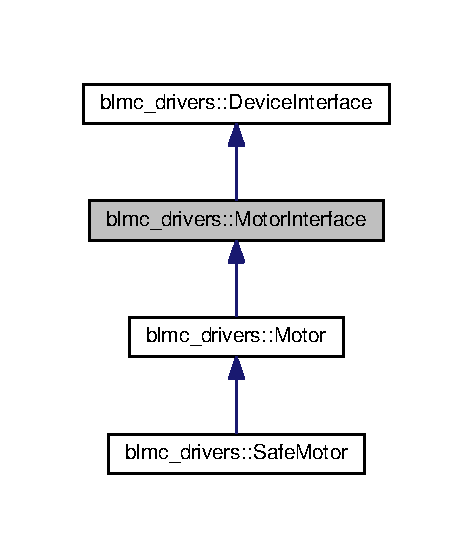
\includegraphics[width=227pt]{classblmc__drivers_1_1MotorInterface__inherit__graph}
\end{center}
\end{figure}


Collaboration diagram for blmc\+\_\+drivers\+:\+:Motor\+Interface\+:
\nopagebreak
\begin{figure}[H]
\begin{center}
\leavevmode
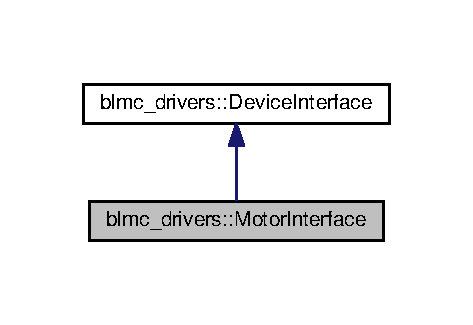
\includegraphics[width=227pt]{classblmc__drivers_1_1MotorInterface__coll__graph}
\end{center}
\end{figure}
\subsection*{Public Types}
\begin{DoxyCompactItemize}
\item 
enum \hyperlink{classblmc__drivers_1_1MotorInterface_a35c1217dd295078c67bacc2cba08ab33}{Measurement\+Index} \{ \\*
{\bfseries current}, 
{\bfseries position}, 
{\bfseries velocity}, 
{\bfseries encoder\+\_\+index}, 
\\*
{\bfseries measurement\+\_\+count}
 \}\hypertarget{classblmc__drivers_1_1MotorInterface_a35c1217dd295078c67bacc2cba08ab33}{}\label{classblmc__drivers_1_1MotorInterface_a35c1217dd295078c67bacc2cba08ab33}
\begin{DoxyCompactList}\small\item\em Here is a list of the different measurement available on the blmc card. \end{DoxyCompactList}
\item 
typedef real\+\_\+time\+\_\+tools\+::\+Threadsafe\+Timeseries$<$ double $>$ \hyperlink{classblmc__drivers_1_1MotorInterface_a49b8fc916b9f9debbd7b0988463db5cd}{Scalar\+Timeseries}\hypertarget{classblmc__drivers_1_1MotorInterface_a49b8fc916b9f9debbd7b0988463db5cd}{}\label{classblmc__drivers_1_1MotorInterface_a49b8fc916b9f9debbd7b0988463db5cd}

\begin{DoxyCompactList}\small\item\em This is a useful alias. \end{DoxyCompactList}\item 
{\footnotesize template$<$typename Type $>$ }\\using \hyperlink{classblmc__drivers_1_1MotorInterface_ae31f230b9da3674a05543023c90b124c}{Ptr} = std\+::shared\+\_\+ptr$<$ Type $>$
\begin{DoxyCompactList}\small\item\em This a useful alias for the shared Pointer creation. \end{DoxyCompactList}\end{DoxyCompactItemize}
\subsection*{Public Member Functions}
\begin{DoxyCompactItemize}
\item 
virtual \hyperlink{classblmc__drivers_1_1MotorInterface_a1f535a7de62ae8246f44541216254da5}{$\sim$\+Motor\+Interface} ()\hypertarget{classblmc__drivers_1_1MotorInterface_a1f535a7de62ae8246f44541216254da5}{}\label{classblmc__drivers_1_1MotorInterface_a1f535a7de62ae8246f44541216254da5}

\begin{DoxyCompactList}\small\item\em Destroy the \hyperlink{classblmc__drivers_1_1MotorInterface}{Motor\+Interface} object. \end{DoxyCompactList}\item 
virtual void \hyperlink{classblmc__drivers_1_1MotorInterface_a7ac16ddd18d76781612714a485dcb6bd}{send\+\_\+if\+\_\+input\+\_\+changed} ()=0\hypertarget{classblmc__drivers_1_1MotorInterface_a7ac16ddd18d76781612714a485dcb6bd}{}\label{classblmc__drivers_1_1MotorInterface_a7ac16ddd18d76781612714a485dcb6bd}

\begin{DoxyCompactList}\small\item\em Actually send the commands and controls. \end{DoxyCompactList}\item 
virtual \hyperlink{classblmc__drivers_1_1MotorInterface_ae31f230b9da3674a05543023c90b124c}{Ptr}$<$ const \hyperlink{classblmc__drivers_1_1MotorInterface_a49b8fc916b9f9debbd7b0988463db5cd}{Scalar\+Timeseries} $>$ \hyperlink{classblmc__drivers_1_1MotorInterface_a7f6afed670f078518ccb46e1e3b44892}{get\+\_\+measurement} (const int \&index=0) const =0
\begin{DoxyCompactList}\small\item\em Getters. \end{DoxyCompactList}\item 
virtual \hyperlink{classblmc__drivers_1_1MotorInterface_ae31f230b9da3674a05543023c90b124c}{Ptr}$<$ const \hyperlink{classblmc__drivers_1_1MotorInterface_a49b8fc916b9f9debbd7b0988463db5cd}{Scalar\+Timeseries} $>$ \hyperlink{classblmc__drivers_1_1MotorInterface_a167ffe5df0412b9abcac9a93861e58d2}{get\+\_\+current\+\_\+target} () const =0
\begin{DoxyCompactList}\small\item\em Get the current target object. \end{DoxyCompactList}\item 
virtual \hyperlink{classblmc__drivers_1_1MotorInterface_ae31f230b9da3674a05543023c90b124c}{Ptr}$<$ const \hyperlink{classblmc__drivers_1_1MotorInterface_a49b8fc916b9f9debbd7b0988463db5cd}{Scalar\+Timeseries} $>$ \hyperlink{classblmc__drivers_1_1MotorInterface_a709804e11aa22fbb3107e781c9799bdb}{get\+\_\+sent\+\_\+current\+\_\+target} () const =0
\begin{DoxyCompactList}\small\item\em Get the history of the sent current targets. \end{DoxyCompactList}\item 
virtual void \hyperlink{classblmc__drivers_1_1MotorInterface_a76b49a1228ad549fa407a54c8da14d13}{set\+\_\+current\+\_\+target} (const double \&current\+\_\+target)=0
\begin{DoxyCompactList}\small\item\em Setters. \end{DoxyCompactList}\item 
virtual void \hyperlink{classblmc__drivers_1_1MotorInterface_a723a772b2be5beb0f07097a5b3e00a89}{set\+\_\+command} (const \hyperlink{classblmc__drivers_1_1MotorBoardCommand}{Motor\+Board\+Command} \&command)=0
\begin{DoxyCompactList}\small\item\em Set the command. \end{DoxyCompactList}\end{DoxyCompactItemize}


\subsection{Detailed Description}
This class declares an interface to the motor. 

It allows the user to access the sensors data as well as sending controls. The only control supported for now is the current. 

\subsection{Member Typedef Documentation}
\index{blmc\+\_\+drivers\+::\+Motor\+Interface@{blmc\+\_\+drivers\+::\+Motor\+Interface}!Ptr@{Ptr}}
\index{Ptr@{Ptr}!blmc\+\_\+drivers\+::\+Motor\+Interface@{blmc\+\_\+drivers\+::\+Motor\+Interface}}
\subsubsection[{\texorpdfstring{Ptr}{Ptr}}]{\setlength{\rightskip}{0pt plus 5cm}template$<$typename Type $>$ using {\bf blmc\+\_\+drivers\+::\+Motor\+Interface\+::\+Ptr} =  std\+::shared\+\_\+ptr$<$Type$>$}\hypertarget{classblmc__drivers_1_1MotorInterface_ae31f230b9da3674a05543023c90b124c}{}\label{classblmc__drivers_1_1MotorInterface_ae31f230b9da3674a05543023c90b124c}


This a useful alias for the shared Pointer creation. 


\begin{DoxyTemplParams}{Template Parameters}
{\em Type} & is the Class to crate the pointer from. \\
\hline
\end{DoxyTemplParams}


\subsection{Member Function Documentation}
\index{blmc\+\_\+drivers\+::\+Motor\+Interface@{blmc\+\_\+drivers\+::\+Motor\+Interface}!get\+\_\+current\+\_\+target@{get\+\_\+current\+\_\+target}}
\index{get\+\_\+current\+\_\+target@{get\+\_\+current\+\_\+target}!blmc\+\_\+drivers\+::\+Motor\+Interface@{blmc\+\_\+drivers\+::\+Motor\+Interface}}
\subsubsection[{\texorpdfstring{get\+\_\+current\+\_\+target() const =0}{get_current_target() const =0}}]{\setlength{\rightskip}{0pt plus 5cm}virtual {\bf Ptr}$<$const {\bf Scalar\+Timeseries}$>$ blmc\+\_\+drivers\+::\+Motor\+Interface\+::get\+\_\+current\+\_\+target (
\begin{DoxyParamCaption}
{}
\end{DoxyParamCaption}
) const\hspace{0.3cm}{\ttfamily [pure virtual]}}\hypertarget{classblmc__drivers_1_1MotorInterface_a167ffe5df0412b9abcac9a93861e58d2}{}\label{classblmc__drivers_1_1MotorInterface_a167ffe5df0412b9abcac9a93861e58d2}


Get the current target object. 

\begin{DoxyReturn}{Returns}
Ptr$<$const Scalar\+Timeseries$>$ the list of the current values to be sent. 
\end{DoxyReturn}


Implemented in \hyperlink{classblmc__drivers_1_1SafeMotor_a2c938b6289e41a7d3ab8a19a045382e0}{blmc\+\_\+drivers\+::\+Safe\+Motor}, and \hyperlink{classblmc__drivers_1_1Motor_ac1c0c4f1faa125bc0b245fdbe2590575}{blmc\+\_\+drivers\+::\+Motor}.

\index{blmc\+\_\+drivers\+::\+Motor\+Interface@{blmc\+\_\+drivers\+::\+Motor\+Interface}!get\+\_\+measurement@{get\+\_\+measurement}}
\index{get\+\_\+measurement@{get\+\_\+measurement}!blmc\+\_\+drivers\+::\+Motor\+Interface@{blmc\+\_\+drivers\+::\+Motor\+Interface}}
\subsubsection[{\texorpdfstring{get\+\_\+measurement(const int \&index=0) const =0}{get_measurement(const int &index=0) const =0}}]{\setlength{\rightskip}{0pt plus 5cm}virtual {\bf Ptr}$<$const {\bf Scalar\+Timeseries}$>$ blmc\+\_\+drivers\+::\+Motor\+Interface\+::get\+\_\+measurement (
\begin{DoxyParamCaption}
\item[{const int \&}]{index = {\ttfamily 0}}
\end{DoxyParamCaption}
) const\hspace{0.3cm}{\ttfamily [pure virtual]}}\hypertarget{classblmc__drivers_1_1MotorInterface_a7f6afed670f078518ccb46e1e3b44892}{}\label{classblmc__drivers_1_1MotorInterface_a7f6afed670f078518ccb46e1e3b44892}


Getters. 

Get the measurements.


\begin{DoxyParams}{Parameters}
{\em index} & \\
\hline
\end{DoxyParams}
\begin{DoxyReturn}{Returns}
Ptr$<$const Scalar\+Timeseries$>$ the pointer to the desired measurement history. 
\end{DoxyReturn}


Implemented in \hyperlink{classblmc__drivers_1_1Motor_a919cb2f48cfc8550fabd5d3c5d7d0cf0}{blmc\+\_\+drivers\+::\+Motor}.

\index{blmc\+\_\+drivers\+::\+Motor\+Interface@{blmc\+\_\+drivers\+::\+Motor\+Interface}!get\+\_\+sent\+\_\+current\+\_\+target@{get\+\_\+sent\+\_\+current\+\_\+target}}
\index{get\+\_\+sent\+\_\+current\+\_\+target@{get\+\_\+sent\+\_\+current\+\_\+target}!blmc\+\_\+drivers\+::\+Motor\+Interface@{blmc\+\_\+drivers\+::\+Motor\+Interface}}
\subsubsection[{\texorpdfstring{get\+\_\+sent\+\_\+current\+\_\+target() const =0}{get_sent_current_target() const =0}}]{\setlength{\rightskip}{0pt plus 5cm}virtual {\bf Ptr}$<$const {\bf Scalar\+Timeseries}$>$ blmc\+\_\+drivers\+::\+Motor\+Interface\+::get\+\_\+sent\+\_\+current\+\_\+target (
\begin{DoxyParamCaption}
{}
\end{DoxyParamCaption}
) const\hspace{0.3cm}{\ttfamily [pure virtual]}}\hypertarget{classblmc__drivers_1_1MotorInterface_a709804e11aa22fbb3107e781c9799bdb}{}\label{classblmc__drivers_1_1MotorInterface_a709804e11aa22fbb3107e781c9799bdb}


Get the history of the sent current targets. 

\begin{DoxyReturn}{Returns}
Ptr$<$const Scalar\+Timeseries$>$ 
\end{DoxyReturn}


Implemented in \hyperlink{classblmc__drivers_1_1Motor_aa629114982c99453b4563a0ec06b9eea}{blmc\+\_\+drivers\+::\+Motor}.

\index{blmc\+\_\+drivers\+::\+Motor\+Interface@{blmc\+\_\+drivers\+::\+Motor\+Interface}!set\+\_\+command@{set\+\_\+command}}
\index{set\+\_\+command@{set\+\_\+command}!blmc\+\_\+drivers\+::\+Motor\+Interface@{blmc\+\_\+drivers\+::\+Motor\+Interface}}
\subsubsection[{\texorpdfstring{set\+\_\+command(const Motor\+Board\+Command \&command)=0}{set_command(const MotorBoardCommand &command)=0}}]{\setlength{\rightskip}{0pt plus 5cm}virtual void blmc\+\_\+drivers\+::\+Motor\+Interface\+::set\+\_\+command (
\begin{DoxyParamCaption}
\item[{const {\bf Motor\+Board\+Command} \&}]{command}
\end{DoxyParamCaption}
)\hspace{0.3cm}{\ttfamily [pure virtual]}}\hypertarget{classblmc__drivers_1_1MotorInterface_a723a772b2be5beb0f07097a5b3e00a89}{}\label{classblmc__drivers_1_1MotorInterface_a723a772b2be5beb0f07097a5b3e00a89}


Set the command. 

Save internally a command to be apply by the motor board. This function save the command internally. Please call \hyperlink{classblmc__drivers_1_1MotorInterface_a7ac16ddd18d76781612714a485dcb6bd}{send\+\_\+if\+\_\+input\+\_\+changed()} to actually send the data.


\begin{DoxyParams}{Parameters}
{\em command} & \\
\hline
\end{DoxyParams}


Implemented in \hyperlink{classblmc__drivers_1_1Motor_a4af56df5466d011fc2a567dd815a6c1b}{blmc\+\_\+drivers\+::\+Motor}.

\index{blmc\+\_\+drivers\+::\+Motor\+Interface@{blmc\+\_\+drivers\+::\+Motor\+Interface}!set\+\_\+current\+\_\+target@{set\+\_\+current\+\_\+target}}
\index{set\+\_\+current\+\_\+target@{set\+\_\+current\+\_\+target}!blmc\+\_\+drivers\+::\+Motor\+Interface@{blmc\+\_\+drivers\+::\+Motor\+Interface}}
\subsubsection[{\texorpdfstring{set\+\_\+current\+\_\+target(const double \&current\+\_\+target)=0}{set_current_target(const double &current_target)=0}}]{\setlength{\rightskip}{0pt plus 5cm}virtual void blmc\+\_\+drivers\+::\+Motor\+Interface\+::set\+\_\+current\+\_\+target (
\begin{DoxyParamCaption}
\item[{const double \&}]{current\+\_\+target}
\end{DoxyParamCaption}
)\hspace{0.3cm}{\ttfamily [pure virtual]}}\hypertarget{classblmc__drivers_1_1MotorInterface_a76b49a1228ad549fa407a54c8da14d13}{}\label{classblmc__drivers_1_1MotorInterface_a76b49a1228ad549fa407a54c8da14d13}


Setters. 

Set the current target. This function saves the data internally. Please call \hyperlink{classblmc__drivers_1_1MotorInterface_a7ac16ddd18d76781612714a485dcb6bd}{send\+\_\+if\+\_\+input\+\_\+changed()} to actually send the data.


\begin{DoxyParams}{Parameters}
{\em current\+\_\+target} & \\
\hline
\end{DoxyParams}


Implemented in \hyperlink{classblmc__drivers_1_1SafeMotor_adedaee24408b94b3d1ed8f856e218b12}{blmc\+\_\+drivers\+::\+Safe\+Motor}, and \hyperlink{classblmc__drivers_1_1Motor_a48801c9858a7b1784b0a0ac4272fdaf5}{blmc\+\_\+drivers\+::\+Motor}.



The documentation for this class was generated from the following file\+:\begin{DoxyCompactItemize}
\item 
include/blmc\+\_\+drivers/devices/\hyperlink{motor_8hpp}{motor.\+hpp}\end{DoxyCompactItemize}

\hypertarget{classblmc__drivers_1_1PDController}{}\section{blmc\+\_\+drivers\+:\+:P\+D\+Controller Class Reference}
\label{classblmc__drivers_1_1PDController}\index{blmc\+\_\+drivers\+::\+P\+D\+Controller@{blmc\+\_\+drivers\+::\+P\+D\+Controller}}


This is a basic PD controller to be used in the demos of this package.  




{\ttfamily \#include $<$pd\+\_\+control.\+hpp$>$}

\subsection*{Public Member Functions}
\begin{DoxyCompactItemize}
\item 
\hyperlink{classblmc__drivers_1_1PDController_a78e3d01f6bcc263b20b81a7525d072cf}{P\+D\+Controller} (std\+::vector$<$ \hyperlink{namespaceblmc__drivers_a134270c90d29a9a28b64ab0e5f7158f7}{Pair\+Motor\+Slider} $>$ motor\+\_\+slider\+\_\+pairs)
\begin{DoxyCompactList}\small\item\em Construct a new \hyperlink{classblmc__drivers_1_1PDController}{P\+D\+Controller} object. \end{DoxyCompactList}\item 
\hyperlink{classblmc__drivers_1_1PDController_aed8ffc7914eb5976f95936315bcd9c47}{$\sim$\+P\+D\+Controller} ()\hypertarget{classblmc__drivers_1_1PDController_aed8ffc7914eb5976f95936315bcd9c47}{}\label{classblmc__drivers_1_1PDController_aed8ffc7914eb5976f95936315bcd9c47}

\begin{DoxyCompactList}\small\item\em Destroy the \hyperlink{classblmc__drivers_1_1PDController}{P\+D\+Controller} object. \end{DoxyCompactList}\item 
void \hyperlink{classblmc__drivers_1_1PDController_a9c9258e9f1af0f4ca00d2ede682ad511}{start\+\_\+loop} ()\hypertarget{classblmc__drivers_1_1PDController_a9c9258e9f1af0f4ca00d2ede682ad511}{}\label{classblmc__drivers_1_1PDController_a9c9258e9f1af0f4ca00d2ede682ad511}

\begin{DoxyCompactList}\small\item\em This method is a helper to start the thread loop. \end{DoxyCompactList}\end{DoxyCompactItemize}
\subsection*{Private Member Functions}
\begin{DoxyCompactItemize}
\item 
void \hyperlink{classblmc__drivers_1_1PDController_ae00d08095b9ff6b6dfd550c59ba2857a}{loop} ()
\begin{DoxyCompactList}\small\item\em this is a simple control loop which runs at a kilohertz. \end{DoxyCompactList}\end{DoxyCompactItemize}
\subsection*{Static Private Member Functions}
\begin{DoxyCompactItemize}
\item 
static T\+H\+R\+E\+A\+D\+\_\+\+F\+U\+N\+C\+T\+I\+O\+N\+\_\+\+R\+E\+T\+U\+R\+N\+\_\+\+T\+Y\+PE \hyperlink{classblmc__drivers_1_1PDController_aaae22ea8cb0324570926c16b43885948}{loop} (void $\ast$instance\+\_\+pointer)\hypertarget{classblmc__drivers_1_1PDController_aaae22ea8cb0324570926c16b43885948}{}\label{classblmc__drivers_1_1PDController_aaae22ea8cb0324570926c16b43885948}

\begin{DoxyCompactList}\small\item\em this function is just a wrapper around the actual loop function, such that it can be spawned as a posix thread. \end{DoxyCompactList}\end{DoxyCompactItemize}
\subsection*{Private Attributes}
\begin{DoxyCompactItemize}
\item 
std\+::vector$<$ \hyperlink{namespaceblmc__drivers_a134270c90d29a9a28b64ab0e5f7158f7}{Pair\+Motor\+Slider} $>$ \hyperlink{classblmc__drivers_1_1PDController_a11b0e1df638bc792b752349f39187a67}{motor\+\_\+slider\+\_\+pairs\+\_\+}\hypertarget{classblmc__drivers_1_1PDController_a11b0e1df638bc792b752349f39187a67}{}\label{classblmc__drivers_1_1PDController_a11b0e1df638bc792b752349f39187a67}

\begin{DoxyCompactList}\small\item\em This is a pair of motor and sliders so that we associate one with the other. \end{DoxyCompactList}\item 
real\+\_\+time\+\_\+tools\+::\+Real\+Time\+Thread \hyperlink{classblmc__drivers_1_1PDController_a425d7f9c093a0c586ef608d4c11c8889}{rt\+\_\+thread\+\_\+}\hypertarget{classblmc__drivers_1_1PDController_a425d7f9c093a0c586ef608d4c11c8889}{}\label{classblmc__drivers_1_1PDController_a425d7f9c093a0c586ef608d4c11c8889}

\begin{DoxyCompactList}\small\item\em This is the real time thread object. \end{DoxyCompactList}\item 
bool \hyperlink{classblmc__drivers_1_1PDController_a3520dd968bde954399bf3ef4508c3d54}{stop\+\_\+loop}\hypertarget{classblmc__drivers_1_1PDController_a3520dd968bde954399bf3ef4508c3d54}{}\label{classblmc__drivers_1_1PDController_a3520dd968bde954399bf3ef4508c3d54}

\begin{DoxyCompactList}\small\item\em managing the stopping of the loop \end{DoxyCompactList}\end{DoxyCompactItemize}


\subsection{Detailed Description}
This is a basic PD controller to be used in the demos of this package. 

\subsection{Constructor \& Destructor Documentation}
\index{blmc\+\_\+drivers\+::\+P\+D\+Controller@{blmc\+\_\+drivers\+::\+P\+D\+Controller}!P\+D\+Controller@{P\+D\+Controller}}
\index{P\+D\+Controller@{P\+D\+Controller}!blmc\+\_\+drivers\+::\+P\+D\+Controller@{blmc\+\_\+drivers\+::\+P\+D\+Controller}}
\subsubsection[{\texorpdfstring{P\+D\+Controller(std\+::vector$<$ Pair\+Motor\+Slider $>$ motor\+\_\+slider\+\_\+pairs)}{PDController(std::vector< PairMotorSlider > motor_slider_pairs)}}]{\setlength{\rightskip}{0pt plus 5cm}blmc\+\_\+drivers\+::\+P\+D\+Controller\+::\+P\+D\+Controller (
\begin{DoxyParamCaption}
\item[{std\+::vector$<$ {\bf Pair\+Motor\+Slider} $>$}]{motor\+\_\+slider\+\_\+pairs}
\end{DoxyParamCaption}
)\hspace{0.3cm}{\ttfamily [inline]}}\hypertarget{classblmc__drivers_1_1PDController_a78e3d01f6bcc263b20b81a7525d072cf}{}\label{classblmc__drivers_1_1PDController_a78e3d01f6bcc263b20b81a7525d072cf}


Construct a new \hyperlink{classblmc__drivers_1_1PDController}{P\+D\+Controller} object. 


\begin{DoxyParams}{Parameters}
{\em motor\+\_\+slider\+\_\+pairs} & \\
\hline
\end{DoxyParams}


\subsection{Member Function Documentation}
\index{blmc\+\_\+drivers\+::\+P\+D\+Controller@{blmc\+\_\+drivers\+::\+P\+D\+Controller}!loop@{loop}}
\index{loop@{loop}!blmc\+\_\+drivers\+::\+P\+D\+Controller@{blmc\+\_\+drivers\+::\+P\+D\+Controller}}
\subsubsection[{\texorpdfstring{loop()}{loop()}}]{\setlength{\rightskip}{0pt plus 5cm}void blmc\+\_\+drivers\+::\+P\+D\+Controller\+::loop (
\begin{DoxyParamCaption}
{}
\end{DoxyParamCaption}
)\hspace{0.3cm}{\ttfamily [private]}}\hypertarget{classblmc__drivers_1_1PDController_ae00d08095b9ff6b6dfd550c59ba2857a}{}\label{classblmc__drivers_1_1PDController_ae00d08095b9ff6b6dfd550c59ba2857a}


this is a simple control loop which runs at a kilohertz. 

it reads the measurement from the analog sensor, in this case the slider. then it scales it and sends it as the current target to the motor. 

The documentation for this class was generated from the following files\+:\begin{DoxyCompactItemize}
\item 
demos/\hyperlink{pd__control_8hpp}{pd\+\_\+control.\+hpp}\item 
demos/\hyperlink{pd__control_8cpp}{pd\+\_\+control.\+cpp}\end{DoxyCompactItemize}

\hypertarget{classblmc__drivers_1_1SafeMotor}{}\section{blmc\+\_\+drivers\+:\+:Safe\+Motor Class Reference}
\label{classblmc__drivers_1_1SafeMotor}\index{blmc\+\_\+drivers\+::\+Safe\+Motor@{blmc\+\_\+drivers\+::\+Safe\+Motor}}


This class is a safe implementation of the \hyperlink{classblmc__drivers_1_1Motor}{Motor} class.  




{\ttfamily \#include $<$motor.\+hpp$>$}



Inheritance diagram for blmc\+\_\+drivers\+:\+:Safe\+Motor\+:
\nopagebreak
\begin{figure}[H]
\begin{center}
\leavevmode
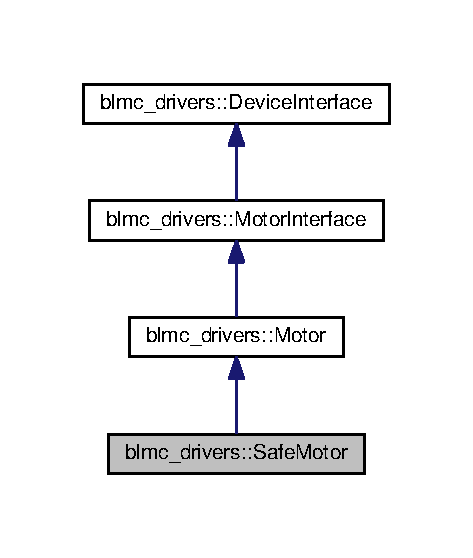
\includegraphics[width=227pt]{classblmc__drivers_1_1SafeMotor__inherit__graph}
\end{center}
\end{figure}


Collaboration diagram for blmc\+\_\+drivers\+:\+:Safe\+Motor\+:
\nopagebreak
\begin{figure}[H]
\begin{center}
\leavevmode
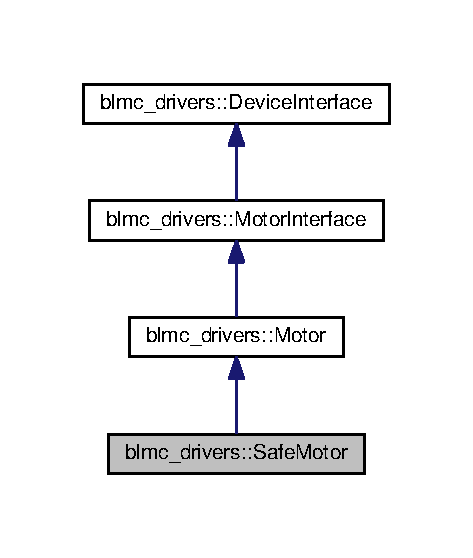
\includegraphics[width=227pt]{classblmc__drivers_1_1SafeMotor__coll__graph}
\end{center}
\end{figure}
\subsection*{Public Member Functions}
\begin{DoxyCompactItemize}
\item 
\hyperlink{classblmc__drivers_1_1SafeMotor_a6e9cda054c161d28f062955d97e73f82}{Safe\+Motor} (\hyperlink{classblmc__drivers_1_1MotorInterface_ae31f230b9da3674a05543023c90b124c}{Ptr}$<$ \hyperlink{classblmc__drivers_1_1MotorBoardInterface}{Motor\+Board\+Interface} $>$ board, bool motor\+\_\+id, const double \&max\+\_\+current\+\_\+target=2.\+0, const size\+\_\+t \&history\+\_\+length=1000, const double \&max\+\_\+velocity=std\+::numeric\+\_\+limits$<$ double $>$\+::quiet\+\_\+\+NaN())
\begin{DoxyCompactList}\small\item\em Construct a new \hyperlink{classblmc__drivers_1_1SafeMotor}{Safe\+Motor} object. \end{DoxyCompactList}\item 
virtual \hyperlink{classblmc__drivers_1_1MotorInterface_ae31f230b9da3674a05543023c90b124c}{Ptr}$<$ const \hyperlink{classblmc__drivers_1_1MotorInterface_a49b8fc916b9f9debbd7b0988463db5cd}{Scalar\+Timeseries} $>$ \hyperlink{classblmc__drivers_1_1SafeMotor_a2c938b6289e41a7d3ab8a19a045382e0}{get\+\_\+current\+\_\+target} () const 
\begin{DoxyCompactList}\small\item\em Getters. \end{DoxyCompactList}\item 
virtual void \hyperlink{classblmc__drivers_1_1SafeMotor_adedaee24408b94b3d1ed8f856e218b12}{set\+\_\+current\+\_\+target} (const double \&current\+\_\+target)
\begin{DoxyCompactList}\small\item\em Setters. \end{DoxyCompactList}\item 
void \hyperlink{classblmc__drivers_1_1SafeMotor_ad4f4bb531e2a9e7f965b319afb53d43c}{set\+\_\+max\+\_\+current} (double max\+\_\+current\+\_\+target)
\begin{DoxyCompactList}\small\item\em Set the max\+\_\+current\+\_\+target\+\_\+ object. \end{DoxyCompactList}\item 
void \hyperlink{classblmc__drivers_1_1SafeMotor_aaa0083a39d815d7b3cd38c680bfea48a}{set\+\_\+max\+\_\+velocity} (double max\+\_\+velocity)
\begin{DoxyCompactList}\small\item\em Set the max\+\_\+velocity\+\_\+ constant. \end{DoxyCompactList}\end{DoxyCompactItemize}
\subsection*{Private Attributes}
\begin{DoxyCompactItemize}
\item 
double \hyperlink{classblmc__drivers_1_1SafeMotor_ae58230855ac502d9c702304d785eb833}{max\+\_\+current\+\_\+target\+\_\+}\hypertarget{classblmc__drivers_1_1SafeMotor_ae58230855ac502d9c702304d785eb833}{}\label{classblmc__drivers_1_1SafeMotor_ae58230855ac502d9c702304d785eb833}

\begin{DoxyCompactList}\small\item\em max\+\_\+current\+\_\+target\+\_\+ is the limit of the current. \end{DoxyCompactList}\item 
double \hyperlink{classblmc__drivers_1_1SafeMotor_a1885b2a1c298765cae0a7ccda75d5f3f}{max\+\_\+velocity\+\_\+}\hypertarget{classblmc__drivers_1_1SafeMotor_a1885b2a1c298765cae0a7ccda75d5f3f}{}\label{classblmc__drivers_1_1SafeMotor_a1885b2a1c298765cae0a7ccda75d5f3f}

\begin{DoxyCompactList}\small\item\em max\+\_\+velocity\+\_\+ limits the motor velocity. \end{DoxyCompactList}\item 
\hyperlink{classblmc__drivers_1_1MotorInterface_ae31f230b9da3674a05543023c90b124c}{Ptr}$<$ \hyperlink{classblmc__drivers_1_1MotorInterface_a49b8fc916b9f9debbd7b0988463db5cd}{Scalar\+Timeseries} $>$ \hyperlink{classblmc__drivers_1_1SafeMotor_af79e6910868177f18a498ea83b350e3f}{current\+\_\+target\+\_\+}\hypertarget{classblmc__drivers_1_1SafeMotor_af79e6910868177f18a498ea83b350e3f}{}\label{classblmc__drivers_1_1SafeMotor_af79e6910868177f18a498ea83b350e3f}

\begin{DoxyCompactList}\small\item\em History of the target current sent. \end{DoxyCompactList}\end{DoxyCompactItemize}
\subsection*{Additional Inherited Members}


\subsection{Detailed Description}
This class is a safe implementation of the \hyperlink{classblmc__drivers_1_1Motor}{Motor} class. 

It contains utilities to bound the control input. It could also contains some velocity limits at the motor level and why not some temperature management.

\begin{DoxyRefDesc}{Todo}
\item[\hyperlink{todo__todo000002}{Todo}]the velocity limit should be implemented in a smoother way, and the parameters should be passed in the constructor. \end{DoxyRefDesc}


\subsection{Constructor \& Destructor Documentation}
\index{blmc\+\_\+drivers\+::\+Safe\+Motor@{blmc\+\_\+drivers\+::\+Safe\+Motor}!Safe\+Motor@{Safe\+Motor}}
\index{Safe\+Motor@{Safe\+Motor}!blmc\+\_\+drivers\+::\+Safe\+Motor@{blmc\+\_\+drivers\+::\+Safe\+Motor}}
\subsubsection[{\texorpdfstring{Safe\+Motor(\+Ptr$<$ Motor\+Board\+Interface $>$ board, bool motor\+\_\+id, const double \&max\+\_\+current\+\_\+target=2.\+0, const size\+\_\+t \&history\+\_\+length=1000, const double \&max\+\_\+velocity=std\+::numeric\+\_\+limits$<$ double $>$\+::quiet\+\_\+\+Na\+N())}{SafeMotor(Ptr< MotorBoardInterface > board, bool motor_id, const double &max_current_target=2.0, const size_t &history_length=1000, const double &max_velocity=std::numeric_limits< double >::quiet_NaN())}}]{\setlength{\rightskip}{0pt plus 5cm}blmc\+\_\+drivers\+::\+Safe\+Motor\+::\+Safe\+Motor (
\begin{DoxyParamCaption}
\item[{{\bf Motor\+::\+Ptr}$<$ {\bf Motor\+Board\+Interface} $>$}]{board, }
\item[{bool}]{motor\+\_\+id, }
\item[{const double \&}]{max\+\_\+current\+\_\+target = {\ttfamily 2.0}, }
\item[{const size\+\_\+t \&}]{history\+\_\+length = {\ttfamily 1000}, }
\item[{const double \&}]{max\+\_\+velocity = {\ttfamily std\+:\+:numeric\+\_\+limits$<$~double$>$\+:\+:quiet\+\_\+NaN()}}
\end{DoxyParamCaption}
)}\hypertarget{classblmc__drivers_1_1SafeMotor_a6e9cda054c161d28f062955d97e73f82}{}\label{classblmc__drivers_1_1SafeMotor_a6e9cda054c161d28f062955d97e73f82}


Construct a new \hyperlink{classblmc__drivers_1_1SafeMotor}{Safe\+Motor} object. 


\begin{DoxyParams}{Parameters}
{\em board} & \\
\hline
{\em motor\+\_\+id} & \\
\hline
{\em max\+\_\+current\+\_\+target} & \\
\hline
{\em history\+\_\+length} & \\
\hline
\end{DoxyParams}


\subsection{Member Function Documentation}
\index{blmc\+\_\+drivers\+::\+Safe\+Motor@{blmc\+\_\+drivers\+::\+Safe\+Motor}!get\+\_\+current\+\_\+target@{get\+\_\+current\+\_\+target}}
\index{get\+\_\+current\+\_\+target@{get\+\_\+current\+\_\+target}!blmc\+\_\+drivers\+::\+Safe\+Motor@{blmc\+\_\+drivers\+::\+Safe\+Motor}}
\subsubsection[{\texorpdfstring{get\+\_\+current\+\_\+target() const }{get_current_target() const }}]{\setlength{\rightskip}{0pt plus 5cm}virtual {\bf Ptr}$<$const {\bf Scalar\+Timeseries}$>$ blmc\+\_\+drivers\+::\+Safe\+Motor\+::get\+\_\+current\+\_\+target (
\begin{DoxyParamCaption}
{}
\end{DoxyParamCaption}
) const\hspace{0.3cm}{\ttfamily [inline]}, {\ttfamily [virtual]}}\hypertarget{classblmc__drivers_1_1SafeMotor_a2c938b6289e41a7d3ab8a19a045382e0}{}\label{classblmc__drivers_1_1SafeMotor_a2c938b6289e41a7d3ab8a19a045382e0}


Getters. 

Get the \+\_\+current\+\_\+target object

\begin{DoxyReturn}{Returns}
Ptr$<$const Scalar\+Timeseries$>$ 
\end{DoxyReturn}


Reimplemented from \hyperlink{classblmc__drivers_1_1Motor_ac1c0c4f1faa125bc0b245fdbe2590575}{blmc\+\_\+drivers\+::\+Motor}.

\index{blmc\+\_\+drivers\+::\+Safe\+Motor@{blmc\+\_\+drivers\+::\+Safe\+Motor}!set\+\_\+current\+\_\+target@{set\+\_\+current\+\_\+target}}
\index{set\+\_\+current\+\_\+target@{set\+\_\+current\+\_\+target}!blmc\+\_\+drivers\+::\+Safe\+Motor@{blmc\+\_\+drivers\+::\+Safe\+Motor}}
\subsubsection[{\texorpdfstring{set\+\_\+current\+\_\+target(const double \&current\+\_\+target)}{set_current_target(const double &current_target)}}]{\setlength{\rightskip}{0pt plus 5cm}void blmc\+\_\+drivers\+::\+Safe\+Motor\+::set\+\_\+current\+\_\+target (
\begin{DoxyParamCaption}
\item[{const double \&}]{current\+\_\+target}
\end{DoxyParamCaption}
)\hspace{0.3cm}{\ttfamily [virtual]}}\hypertarget{classblmc__drivers_1_1SafeMotor_adedaee24408b94b3d1ed8f856e218b12}{}\label{classblmc__drivers_1_1SafeMotor_adedaee24408b94b3d1ed8f856e218b12}


Setters. 

Set the current target (Ampere)


\begin{DoxyParams}{Parameters}
{\em current\+\_\+target} & \\
\hline
\end{DoxyParams}


Reimplemented from \hyperlink{classblmc__drivers_1_1Motor_a48801c9858a7b1784b0a0ac4272fdaf5}{blmc\+\_\+drivers\+::\+Motor}.

\index{blmc\+\_\+drivers\+::\+Safe\+Motor@{blmc\+\_\+drivers\+::\+Safe\+Motor}!set\+\_\+max\+\_\+current@{set\+\_\+max\+\_\+current}}
\index{set\+\_\+max\+\_\+current@{set\+\_\+max\+\_\+current}!blmc\+\_\+drivers\+::\+Safe\+Motor@{blmc\+\_\+drivers\+::\+Safe\+Motor}}
\subsubsection[{\texorpdfstring{set\+\_\+max\+\_\+current(double max\+\_\+current\+\_\+target)}{set_max_current(double max_current_target)}}]{\setlength{\rightskip}{0pt plus 5cm}void blmc\+\_\+drivers\+::\+Safe\+Motor\+::set\+\_\+max\+\_\+current (
\begin{DoxyParamCaption}
\item[{double}]{max\+\_\+current\+\_\+target}
\end{DoxyParamCaption}
)\hspace{0.3cm}{\ttfamily [inline]}}\hypertarget{classblmc__drivers_1_1SafeMotor_ad4f4bb531e2a9e7f965b319afb53d43c}{}\label{classblmc__drivers_1_1SafeMotor_ad4f4bb531e2a9e7f965b319afb53d43c}


Set the max\+\_\+current\+\_\+target\+\_\+ object. 


\begin{DoxyParams}{Parameters}
{\em max\+\_\+current\+\_\+target} & \\
\hline
\end{DoxyParams}
\index{blmc\+\_\+drivers\+::\+Safe\+Motor@{blmc\+\_\+drivers\+::\+Safe\+Motor}!set\+\_\+max\+\_\+velocity@{set\+\_\+max\+\_\+velocity}}
\index{set\+\_\+max\+\_\+velocity@{set\+\_\+max\+\_\+velocity}!blmc\+\_\+drivers\+::\+Safe\+Motor@{blmc\+\_\+drivers\+::\+Safe\+Motor}}
\subsubsection[{\texorpdfstring{set\+\_\+max\+\_\+velocity(double max\+\_\+velocity)}{set_max_velocity(double max_velocity)}}]{\setlength{\rightskip}{0pt plus 5cm}void blmc\+\_\+drivers\+::\+Safe\+Motor\+::set\+\_\+max\+\_\+velocity (
\begin{DoxyParamCaption}
\item[{double}]{max\+\_\+velocity}
\end{DoxyParamCaption}
)\hspace{0.3cm}{\ttfamily [inline]}}\hypertarget{classblmc__drivers_1_1SafeMotor_aaa0083a39d815d7b3cd38c680bfea48a}{}\label{classblmc__drivers_1_1SafeMotor_aaa0083a39d815d7b3cd38c680bfea48a}


Set the max\+\_\+velocity\+\_\+ constant. 


\begin{DoxyParams}{Parameters}
{\em max\+\_\+velocity} & \\
\hline
\end{DoxyParams}


The documentation for this class was generated from the following files\+:\begin{DoxyCompactItemize}
\item 
include/blmc\+\_\+drivers/devices/\hyperlink{motor_8hpp}{motor.\+hpp}\item 
src/\hyperlink{motor_8cpp}{motor.\+cpp}\end{DoxyCompactItemize}

\hypertarget{classblmc__drivers_1_1SerialReader}{}\section{blmc\+\_\+drivers\+:\+:Serial\+Reader Class Reference}
\label{classblmc__drivers_1_1SerialReader}\index{blmc\+\_\+drivers\+::\+Serial\+Reader@{blmc\+\_\+drivers\+::\+Serial\+Reader}}
\subsection*{Public Member Functions}
\begin{DoxyCompactItemize}
\item 
\hyperlink{classblmc__drivers_1_1SerialReader_a894216b6799b0ea9945f8a1cf98f9801}{Serial\+Reader} (const std\+::string \&serial\+\_\+port, const int \&num\+\_\+values)
\item 
int \hyperlink{classblmc__drivers_1_1SerialReader_aa590c82f97cfa6d9222bc3d19952f166}{fill\+\_\+vector} (std\+::vector$<$ int $>$ \&values)
\begin{DoxyCompactList}\small\item\em Fills a vector with the latest values. \end{DoxyCompactList}\end{DoxyCompactItemize}
\subsection*{Private Member Functions}
\begin{DoxyCompactItemize}
\item 
void \hyperlink{classblmc__drivers_1_1SerialReader_a24a8f28fa8e56934baa1d0b9fef7a045}{loop} ()\hypertarget{classblmc__drivers_1_1SerialReader_a24a8f28fa8e56934baa1d0b9fef7a045}{}\label{classblmc__drivers_1_1SerialReader_a24a8f28fa8e56934baa1d0b9fef7a045}

\begin{DoxyCompactList}\small\item\em This is the real time thread that streams the data to/from the main board. \end{DoxyCompactList}\end{DoxyCompactItemize}
\subsection*{Static Private Member Functions}
\begin{DoxyCompactItemize}
\item 
static T\+H\+R\+E\+A\+D\+\_\+\+F\+U\+N\+C\+T\+I\+O\+N\+\_\+\+R\+E\+T\+U\+R\+N\+\_\+\+T\+Y\+PE \hyperlink{classblmc__drivers_1_1SerialReader_aaa18311d9c274b0ac8a8bd86a311d3fc}{loop} (void $\ast$instance\+\_\+pointer)
\begin{DoxyCompactList}\small\item\em This is the helper function used for spawning the real time thread. \end{DoxyCompactList}\end{DoxyCompactItemize}
\subsection*{Private Attributes}
\begin{DoxyCompactItemize}
\item 
bool \hyperlink{classblmc__drivers_1_1SerialReader_a37e1129c27b41cd9f5b4317081b217d8}{is\+\_\+loop\+\_\+active\+\_\+}\hypertarget{classblmc__drivers_1_1SerialReader_a37e1129c27b41cd9f5b4317081b217d8}{}\label{classblmc__drivers_1_1SerialReader_a37e1129c27b41cd9f5b4317081b217d8}

\begin{DoxyCompactList}\small\item\em This boolean makes sure that the loop is stopped upon destruction of this object. \end{DoxyCompactList}\item 
real\+\_\+time\+\_\+tools\+::\+Real\+Time\+Thread \hyperlink{classblmc__drivers_1_1SerialReader_a89a2a93d8a9e59738f41d8b69cb112d0}{rt\+\_\+thread\+\_\+}\hypertarget{classblmc__drivers_1_1SerialReader_a89a2a93d8a9e59738f41d8b69cb112d0}{}\label{classblmc__drivers_1_1SerialReader_a89a2a93d8a9e59738f41d8b69cb112d0}

\begin{DoxyCompactList}\small\item\em This is the thread object that allow to spwan a real-\/time thread or not dependening on the current OS. \end{DoxyCompactList}\item 
int \hyperlink{classblmc__drivers_1_1SerialReader_abf30ca34b8f61706a763a431dff68e94}{fd\+\_\+}\hypertarget{classblmc__drivers_1_1SerialReader_abf30ca34b8f61706a763a431dff68e94}{}\label{classblmc__drivers_1_1SerialReader_abf30ca34b8f61706a763a431dff68e94}

\begin{DoxyCompactList}\small\item\em Holds the device serial port. \end{DoxyCompactList}\item 
bool \hyperlink{classblmc__drivers_1_1SerialReader_abb0700e8e752917876798db18a0421db}{has\+\_\+error\+\_\+}\hypertarget{classblmc__drivers_1_1SerialReader_abb0700e8e752917876798db18a0421db}{}\label{classblmc__drivers_1_1SerialReader_abb0700e8e752917876798db18a0421db}

\begin{DoxyCompactList}\small\item\em If false, the communication is workinng as expected. \end{DoxyCompactList}\item 
bool \hyperlink{classblmc__drivers_1_1SerialReader_abf6fd962e185be25e6c61c63f8eb0cc9}{is\+\_\+active\+\_\+}\hypertarget{classblmc__drivers_1_1SerialReader_abf6fd962e185be25e6c61c63f8eb0cc9}{}\label{classblmc__drivers_1_1SerialReader_abf6fd962e185be25e6c61c63f8eb0cc9}

\begin{DoxyCompactList}\small\item\em If the communication is active. \end{DoxyCompactList}\item 
int {\bfseries new\+\_\+data\+\_\+counter\+\_\+}\hypertarget{classblmc__drivers_1_1SerialReader_a862829c3e7f3c59b1e3be49b61e6cfb5}{}\label{classblmc__drivers_1_1SerialReader_a862829c3e7f3c59b1e3be49b61e6cfb5}

\item 
int {\bfseries missed\+\_\+data\+\_\+counter\+\_\+}\hypertarget{classblmc__drivers_1_1SerialReader_a516bbec3112f46bb6442858d2d9446bf}{}\label{classblmc__drivers_1_1SerialReader_a516bbec3112f46bb6442858d2d9446bf}

\item 
std\+::vector$<$ int $>$ \hyperlink{classblmc__drivers_1_1SerialReader_ac6f46fc37c9ce41908ad76b012d2160b}{latest\+\_\+values\+\_\+}\hypertarget{classblmc__drivers_1_1SerialReader_ac6f46fc37c9ce41908ad76b012d2160b}{}\label{classblmc__drivers_1_1SerialReader_ac6f46fc37c9ce41908ad76b012d2160b}

\begin{DoxyCompactList}\small\item\em Holds vector with the latest double values. \end{DoxyCompactList}\item 
std\+::mutex \hyperlink{classblmc__drivers_1_1SerialReader_a38d2ba095d199db4ae9858b888ef20de}{mutex\+\_\+}\hypertarget{classblmc__drivers_1_1SerialReader_a38d2ba095d199db4ae9858b888ef20de}{}\label{classblmc__drivers_1_1SerialReader_a38d2ba095d199db4ae9858b888ef20de}

\begin{DoxyCompactList}\small\item\em mutex\+\_\+ multithreading safety \end{DoxyCompactList}\end{DoxyCompactItemize}


\subsection{Constructor \& Destructor Documentation}
\index{blmc\+\_\+drivers\+::\+Serial\+Reader@{blmc\+\_\+drivers\+::\+Serial\+Reader}!Serial\+Reader@{Serial\+Reader}}
\index{Serial\+Reader@{Serial\+Reader}!blmc\+\_\+drivers\+::\+Serial\+Reader@{blmc\+\_\+drivers\+::\+Serial\+Reader}}
\subsubsection[{\texorpdfstring{Serial\+Reader(const std\+::string \&serial\+\_\+port, const int \&num\+\_\+values)}{SerialReader(const std::string &serial_port, const int &num_values)}}]{\setlength{\rightskip}{0pt plus 5cm}blmc\+\_\+drivers\+::\+Serial\+Reader\+::\+Serial\+Reader (
\begin{DoxyParamCaption}
\item[{const std\+::string \&}]{serial\+\_\+port, }
\item[{const int \&}]{num\+\_\+values}
\end{DoxyParamCaption}
)}\hypertarget{classblmc__drivers_1_1SerialReader_a894216b6799b0ea9945f8a1cf98f9801}{}\label{classblmc__drivers_1_1SerialReader_a894216b6799b0ea9945f8a1cf98f9801}

\begin{DoxyParams}{Parameters}
{\em serial\+\_\+port} & The address of the serial port to use.  num\+\_\+values The number of values to read in each line. \\
\hline
\end{DoxyParams}


\subsection{Member Function Documentation}
\index{blmc\+\_\+drivers\+::\+Serial\+Reader@{blmc\+\_\+drivers\+::\+Serial\+Reader}!fill\+\_\+vector@{fill\+\_\+vector}}
\index{fill\+\_\+vector@{fill\+\_\+vector}!blmc\+\_\+drivers\+::\+Serial\+Reader@{blmc\+\_\+drivers\+::\+Serial\+Reader}}
\subsubsection[{\texorpdfstring{fill\+\_\+vector(std\+::vector$<$ int $>$ \&values)}{fill_vector(std::vector< int > &values)}}]{\setlength{\rightskip}{0pt plus 5cm}int blmc\+\_\+drivers\+::\+Serial\+Reader\+::fill\+\_\+vector (
\begin{DoxyParamCaption}
\item[{std\+::vector$<$ int $>$ \&}]{values}
\end{DoxyParamCaption}
)}\hypertarget{classblmc__drivers_1_1SerialReader_aa590c82f97cfa6d9222bc3d19952f166}{}\label{classblmc__drivers_1_1SerialReader_aa590c82f97cfa6d9222bc3d19952f166}


Fills a vector with the latest values. 


\begin{DoxyParams}{Parameters}
{\em values} & Vector to place values into. \\
\hline
\end{DoxyParams}
\begin{DoxyReturn}{Returns}
How often fill\+\_\+vector was called without new data. 
\end{DoxyReturn}
\index{blmc\+\_\+drivers\+::\+Serial\+Reader@{blmc\+\_\+drivers\+::\+Serial\+Reader}!loop@{loop}}
\index{loop@{loop}!blmc\+\_\+drivers\+::\+Serial\+Reader@{blmc\+\_\+drivers\+::\+Serial\+Reader}}
\subsubsection[{\texorpdfstring{loop(void $\ast$instance\+\_\+pointer)}{loop(void *instance_pointer)}}]{\setlength{\rightskip}{0pt plus 5cm}static T\+H\+R\+E\+A\+D\+\_\+\+F\+U\+N\+C\+T\+I\+O\+N\+\_\+\+R\+E\+T\+U\+R\+N\+\_\+\+T\+Y\+PE blmc\+\_\+drivers\+::\+Serial\+Reader\+::loop (
\begin{DoxyParamCaption}
\item[{void $\ast$}]{instance\+\_\+pointer}
\end{DoxyParamCaption}
)\hspace{0.3cm}{\ttfamily [inline]}, {\ttfamily [static]}, {\ttfamily [private]}}\hypertarget{classblmc__drivers_1_1SerialReader_aaa18311d9c274b0ac8a8bd86a311d3fc}{}\label{classblmc__drivers_1_1SerialReader_aaa18311d9c274b0ac8a8bd86a311d3fc}


This is the helper function used for spawning the real time thread. 


\begin{DoxyParams}{Parameters}
{\em instance\+\_\+pointer} & is the current object in this case. \\
\hline
\end{DoxyParams}
\begin{DoxyReturn}{Returns}
T\+H\+R\+E\+A\+D\+\_\+\+F\+U\+N\+C\+T\+I\+O\+N\+\_\+\+R\+E\+T\+U\+R\+N\+\_\+\+T\+Y\+PE depends on the current OS. 
\end{DoxyReturn}


The documentation for this class was generated from the following files\+:\begin{DoxyCompactItemize}
\item 
include/blmc\+\_\+drivers/\hyperlink{serial__reader_8hpp}{serial\+\_\+reader.\+hpp}\item 
src/\hyperlink{serial__reader_8cpp}{serial\+\_\+reader.\+cpp}\end{DoxyCompactItemize}

\hypertarget{classblmc__drivers_1_1SinePositionControl}{}\section{blmc\+\_\+drivers\+:\+:Sine\+Position\+Control Class Reference}
\label{classblmc__drivers_1_1SinePositionControl}\index{blmc\+\_\+drivers\+::\+Sine\+Position\+Control@{blmc\+\_\+drivers\+::\+Sine\+Position\+Control}}


This is a basic PD controller to be used in the demos of this package.  




{\ttfamily \#include $<$sine\+\_\+position\+\_\+control.\+hpp$>$}

\subsection*{Public Member Functions}
\begin{DoxyCompactItemize}
\item 
\hyperlink{classblmc__drivers_1_1SinePositionControl_a6f5a006338c7975f9aeef5987384c661}{Sine\+Position\+Control} (std\+::vector$<$ \hyperlink{namespaceblmc__drivers_ab975c3be3c53a93a10c491f07a132e2b}{Safe\+Motor\+\_\+ptr} $>$ motor\+\_\+list)
\begin{DoxyCompactList}\small\item\em Construct a new \hyperlink{classblmc__drivers_1_1SinePositionControl}{Sine\+Position\+Control} object. \end{DoxyCompactList}\item 
\hyperlink{classblmc__drivers_1_1SinePositionControl_a35004249215059c73863e71680b977a8}{$\sim$\+Sine\+Position\+Control} ()\hypertarget{classblmc__drivers_1_1SinePositionControl_a35004249215059c73863e71680b977a8}{}\label{classblmc__drivers_1_1SinePositionControl_a35004249215059c73863e71680b977a8}

\begin{DoxyCompactList}\small\item\em Destroy the \hyperlink{classblmc__drivers_1_1SinePositionControl}{Sine\+Position\+Control} object. \end{DoxyCompactList}\item 
void \hyperlink{classblmc__drivers_1_1SinePositionControl_a0766604ca7e58200e97547e61e0f4cc8}{start\+\_\+loop} ()\hypertarget{classblmc__drivers_1_1SinePositionControl_a0766604ca7e58200e97547e61e0f4cc8}{}\label{classblmc__drivers_1_1SinePositionControl_a0766604ca7e58200e97547e61e0f4cc8}

\begin{DoxyCompactList}\small\item\em This method is a helper to start the thread loop. \end{DoxyCompactList}\item 
void \hyperlink{classblmc__drivers_1_1SinePositionControl_a61875cedee870d5cc0cb5e10799b1c24}{stop\+\_\+loop} ()\hypertarget{classblmc__drivers_1_1SinePositionControl_a61875cedee870d5cc0cb5e10799b1c24}{}\label{classblmc__drivers_1_1SinePositionControl_a61875cedee870d5cc0cb5e10799b1c24}

\begin{DoxyCompactList}\small\item\em Stop the control and dump the data. \end{DoxyCompactList}\item 
void {\bfseries set\+\_\+gains} (double kp, double kd)\hypertarget{classblmc__drivers_1_1SinePositionControl_a0a86810773b5a172cbc5f407fa59df4d}{}\label{classblmc__drivers_1_1SinePositionControl_a0a86810773b5a172cbc5f407fa59df4d}

\end{DoxyCompactItemize}
\subsection*{Private Member Functions}
\begin{DoxyCompactItemize}
\item 
void \hyperlink{classblmc__drivers_1_1SinePositionControl_a1e5ab43762ca2511a6badc7065f47e4b}{loop} ()
\begin{DoxyCompactList}\small\item\em this is a simple control loop which runs at a kilohertz. \end{DoxyCompactList}\end{DoxyCompactItemize}
\subsection*{Static Private Member Functions}
\begin{DoxyCompactItemize}
\item 
static T\+H\+R\+E\+A\+D\+\_\+\+F\+U\+N\+C\+T\+I\+O\+N\+\_\+\+R\+E\+T\+U\+R\+N\+\_\+\+T\+Y\+PE \hyperlink{classblmc__drivers_1_1SinePositionControl_ad24e437d64cd1ac1fca2bc5428c844f4}{loop} (void $\ast$instance\+\_\+pointer)\hypertarget{classblmc__drivers_1_1SinePositionControl_ad24e437d64cd1ac1fca2bc5428c844f4}{}\label{classblmc__drivers_1_1SinePositionControl_ad24e437d64cd1ac1fca2bc5428c844f4}

\begin{DoxyCompactList}\small\item\em this function is just a wrapper around the actual loop function, such that it can be spawned as a posix thread. \end{DoxyCompactList}\end{DoxyCompactItemize}
\subsection*{Private Attributes}
\begin{DoxyCompactItemize}
\item 
std\+::vector$<$ \hyperlink{namespaceblmc__drivers_ab975c3be3c53a93a10c491f07a132e2b}{Safe\+Motor\+\_\+ptr} $>$ \hyperlink{classblmc__drivers_1_1SinePositionControl_af210bec9cf5b60d5f6a481449e65112b}{motor\+\_\+list\+\_\+}\hypertarget{classblmc__drivers_1_1SinePositionControl_af210bec9cf5b60d5f6a481449e65112b}{}\label{classblmc__drivers_1_1SinePositionControl_af210bec9cf5b60d5f6a481449e65112b}

\begin{DoxyCompactList}\small\item\em This is list of motors. \end{DoxyCompactList}\item 
real\+\_\+time\+\_\+tools\+::\+Real\+Time\+Thread \hyperlink{classblmc__drivers_1_1SinePositionControl_a89c0d71051efbc318f80833b3dc50b55}{rt\+\_\+thread\+\_\+}\hypertarget{classblmc__drivers_1_1SinePositionControl_a89c0d71051efbc318f80833b3dc50b55}{}\label{classblmc__drivers_1_1SinePositionControl_a89c0d71051efbc318f80833b3dc50b55}

\begin{DoxyCompactList}\small\item\em This is the real time thread object. \end{DoxyCompactList}\item 
bool \hyperlink{classblmc__drivers_1_1SinePositionControl_a65b832cf1c7762140b79bbac39f42a09}{stop\+\_\+loop\+\_\+}\hypertarget{classblmc__drivers_1_1SinePositionControl_a65b832cf1c7762140b79bbac39f42a09}{}\label{classblmc__drivers_1_1SinePositionControl_a65b832cf1c7762140b79bbac39f42a09}

\begin{DoxyCompactList}\small\item\em managing the stopping of the loop \end{DoxyCompactList}\item 
unsigned \hyperlink{classblmc__drivers_1_1SinePositionControl_a6d934043fd7ef066c5cd680e0c055b58}{memory\+\_\+buffer\+\_\+size\+\_\+}\hypertarget{classblmc__drivers_1_1SinePositionControl_a6d934043fd7ef066c5cd680e0c055b58}{}\label{classblmc__drivers_1_1SinePositionControl_a6d934043fd7ef066c5cd680e0c055b58}

\begin{DoxyCompactList}\small\item\em memory\+\_\+buffer\+\_\+size\+\_\+ is the max size of the memory buffer. \end{DoxyCompactList}\item 
std\+::vector$<$ std\+::deque$<$ double $>$ $>$ \hyperlink{classblmc__drivers_1_1SinePositionControl_a8d9d600b107301dfec87f04615e3721a}{encoders\+\_\+}\hypertarget{classblmc__drivers_1_1SinePositionControl_a8d9d600b107301dfec87f04615e3721a}{}\label{classblmc__drivers_1_1SinePositionControl_a8d9d600b107301dfec87f04615e3721a}

\begin{DoxyCompactList}\small\item\em Encoder data. \end{DoxyCompactList}\item 
std\+::vector$<$ std\+::deque$<$ double $>$ $>$ \hyperlink{classblmc__drivers_1_1SinePositionControl_a1ad95cec3a68d2dff06219dff5f83ab8}{velocities\+\_\+}\hypertarget{classblmc__drivers_1_1SinePositionControl_a1ad95cec3a68d2dff06219dff5f83ab8}{}\label{classblmc__drivers_1_1SinePositionControl_a1ad95cec3a68d2dff06219dff5f83ab8}

\begin{DoxyCompactList}\small\item\em Velocity data. \end{DoxyCompactList}\item 
std\+::vector$<$ std\+::deque$<$ double $>$ $>$ \hyperlink{classblmc__drivers_1_1SinePositionControl_ab7903dd177f6dcaa7efa00591ad656d9}{currents\+\_\+}\hypertarget{classblmc__drivers_1_1SinePositionControl_ab7903dd177f6dcaa7efa00591ad656d9}{}\label{classblmc__drivers_1_1SinePositionControl_ab7903dd177f6dcaa7efa00591ad656d9}

\begin{DoxyCompactList}\small\item\em current data \end{DoxyCompactList}\item 
std\+::vector$<$ std\+::deque$<$ double $>$ $>$ \hyperlink{classblmc__drivers_1_1SinePositionControl_a29bd0da456de8a71467de12a3ab42265}{control\+\_\+buffer\+\_\+}\hypertarget{classblmc__drivers_1_1SinePositionControl_a29bd0da456de8a71467de12a3ab42265}{}\label{classblmc__drivers_1_1SinePositionControl_a29bd0da456de8a71467de12a3ab42265}

\begin{DoxyCompactList}\small\item\em control\+\_\+buffer\+\_\+ \end{DoxyCompactList}\item 
double \hyperlink{classblmc__drivers_1_1SinePositionControl_a1b9b44bf55c548c937b4a8ff06d0102d}{kp\+\_\+}\hypertarget{classblmc__drivers_1_1SinePositionControl_a1b9b44bf55c548c937b4a8ff06d0102d}{}\label{classblmc__drivers_1_1SinePositionControl_a1b9b44bf55c548c937b4a8ff06d0102d}

\begin{DoxyCompactList}\small\item\em \hyperlink{classController}{Controller} proportional gain. \end{DoxyCompactList}\item 
double \hyperlink{classblmc__drivers_1_1SinePositionControl_ab48d1f5927551b7856474b92a84859e9}{kd\+\_\+}\hypertarget{classblmc__drivers_1_1SinePositionControl_ab48d1f5927551b7856474b92a84859e9}{}\label{classblmc__drivers_1_1SinePositionControl_ab48d1f5927551b7856474b92a84859e9}

\begin{DoxyCompactList}\small\item\em \hyperlink{classController}{Controller} derivative gain. \end{DoxyCompactList}\end{DoxyCompactItemize}


\subsection{Detailed Description}
This is a basic PD controller to be used in the demos of this package. 

\subsection{Constructor \& Destructor Documentation}
\index{blmc\+\_\+drivers\+::\+Sine\+Position\+Control@{blmc\+\_\+drivers\+::\+Sine\+Position\+Control}!Sine\+Position\+Control@{Sine\+Position\+Control}}
\index{Sine\+Position\+Control@{Sine\+Position\+Control}!blmc\+\_\+drivers\+::\+Sine\+Position\+Control@{blmc\+\_\+drivers\+::\+Sine\+Position\+Control}}
\subsubsection[{\texorpdfstring{Sine\+Position\+Control(std\+::vector$<$ Safe\+Motor\+\_\+ptr $>$ motor\+\_\+list)}{SinePositionControl(std::vector< SafeMotor_ptr > motor_list)}}]{\setlength{\rightskip}{0pt plus 5cm}blmc\+\_\+drivers\+::\+Sine\+Position\+Control\+::\+Sine\+Position\+Control (
\begin{DoxyParamCaption}
\item[{std\+::vector$<$ {\bf Safe\+Motor\+\_\+ptr} $>$}]{motor\+\_\+list}
\end{DoxyParamCaption}
)\hspace{0.3cm}{\ttfamily [inline]}}\hypertarget{classblmc__drivers_1_1SinePositionControl_a6f5a006338c7975f9aeef5987384c661}{}\label{classblmc__drivers_1_1SinePositionControl_a6f5a006338c7975f9aeef5987384c661}


Construct a new \hyperlink{classblmc__drivers_1_1SinePositionControl}{Sine\+Position\+Control} object. 


\begin{DoxyParams}{Parameters}
{\em motor\+\_\+slider\+\_\+pairs} & \\
\hline
\end{DoxyParams}


\subsection{Member Function Documentation}
\index{blmc\+\_\+drivers\+::\+Sine\+Position\+Control@{blmc\+\_\+drivers\+::\+Sine\+Position\+Control}!loop@{loop}}
\index{loop@{loop}!blmc\+\_\+drivers\+::\+Sine\+Position\+Control@{blmc\+\_\+drivers\+::\+Sine\+Position\+Control}}
\subsubsection[{\texorpdfstring{loop()}{loop()}}]{\setlength{\rightskip}{0pt plus 5cm}void blmc\+\_\+drivers\+::\+Sine\+Position\+Control\+::loop (
\begin{DoxyParamCaption}
{}
\end{DoxyParamCaption}
)\hspace{0.3cm}{\ttfamily [private]}}\hypertarget{classblmc__drivers_1_1SinePositionControl_a1e5ab43762ca2511a6badc7065f47e4b}{}\label{classblmc__drivers_1_1SinePositionControl_a1e5ab43762ca2511a6badc7065f47e4b}


this is a simple control loop which runs at a kilohertz. 

it reads the measurement from the analog sensor, in this case the slider. then it scales it and sends it as the current target to the motor. 

The documentation for this class was generated from the following files\+:\begin{DoxyCompactItemize}
\item 
demos/\hyperlink{sine__position__control_8hpp}{sine\+\_\+position\+\_\+control.\+hpp}\item 
demos/\hyperlink{sine__position__control_8cpp}{sine\+\_\+position\+\_\+control.\+cpp}\end{DoxyCompactItemize}

\hypertarget{classblmc__drivers_1_1SineTorqueControl}{}\section{blmc\+\_\+drivers\+:\+:Sine\+Torque\+Control Class Reference}
\label{classblmc__drivers_1_1SineTorqueControl}\index{blmc\+\_\+drivers\+::\+Sine\+Torque\+Control@{blmc\+\_\+drivers\+::\+Sine\+Torque\+Control}}


This is a basic PD controller to be used in the demos of this package.  




{\ttfamily \#include $<$sine\+\_\+torque\+\_\+control.\+hpp$>$}

\subsection*{Public Member Functions}
\begin{DoxyCompactItemize}
\item 
\hyperlink{classblmc__drivers_1_1SineTorqueControl_ab3fcdb73429a6e4a664dc294f80e6d3c}{Sine\+Torque\+Control} (std\+::vector$<$ \hyperlink{namespaceblmc__drivers_ab975c3be3c53a93a10c491f07a132e2b}{Safe\+Motor\+\_\+ptr} $>$ motor\+\_\+list)
\begin{DoxyCompactList}\small\item\em Construct a new \hyperlink{classblmc__drivers_1_1SineTorqueControl}{Sine\+Torque\+Control} object. \end{DoxyCompactList}\item 
\hyperlink{classblmc__drivers_1_1SineTorqueControl_ae66565e4a8be3eb93d84f6dc0c825ce6}{$\sim$\+Sine\+Torque\+Control} ()\hypertarget{classblmc__drivers_1_1SineTorqueControl_ae66565e4a8be3eb93d84f6dc0c825ce6}{}\label{classblmc__drivers_1_1SineTorqueControl_ae66565e4a8be3eb93d84f6dc0c825ce6}

\begin{DoxyCompactList}\small\item\em Destroy the \hyperlink{classblmc__drivers_1_1SineTorqueControl}{Sine\+Torque\+Control} object. \end{DoxyCompactList}\item 
void \hyperlink{classblmc__drivers_1_1SineTorqueControl_aa884278b4fc524c8e6d93b23630aa967}{start\+\_\+loop} ()\hypertarget{classblmc__drivers_1_1SineTorqueControl_aa884278b4fc524c8e6d93b23630aa967}{}\label{classblmc__drivers_1_1SineTorqueControl_aa884278b4fc524c8e6d93b23630aa967}

\begin{DoxyCompactList}\small\item\em This method is a helper to start the thread loop. \end{DoxyCompactList}\item 
void \hyperlink{classblmc__drivers_1_1SineTorqueControl_a1ecff8c52b3a8b0f6ece6818c42ec94a}{stop\+\_\+loop} ()\hypertarget{classblmc__drivers_1_1SineTorqueControl_a1ecff8c52b3a8b0f6ece6818c42ec94a}{}\label{classblmc__drivers_1_1SineTorqueControl_a1ecff8c52b3a8b0f6ece6818c42ec94a}

\begin{DoxyCompactList}\small\item\em Stop the control and dump the data. \end{DoxyCompactList}\end{DoxyCompactItemize}
\subsection*{Private Member Functions}
\begin{DoxyCompactItemize}
\item 
void \hyperlink{classblmc__drivers_1_1SineTorqueControl_a9f5f27389db0a303e2bae2f9c5135417}{loop} ()
\begin{DoxyCompactList}\small\item\em this is a simple control loop which runs at a kilohertz. \end{DoxyCompactList}\end{DoxyCompactItemize}
\subsection*{Static Private Member Functions}
\begin{DoxyCompactItemize}
\item 
static T\+H\+R\+E\+A\+D\+\_\+\+F\+U\+N\+C\+T\+I\+O\+N\+\_\+\+R\+E\+T\+U\+R\+N\+\_\+\+T\+Y\+PE \hyperlink{classblmc__drivers_1_1SineTorqueControl_a6882e509d6e81f09a70aa4214aeadf16}{loop} (void $\ast$instance\+\_\+pointer)\hypertarget{classblmc__drivers_1_1SineTorqueControl_a6882e509d6e81f09a70aa4214aeadf16}{}\label{classblmc__drivers_1_1SineTorqueControl_a6882e509d6e81f09a70aa4214aeadf16}

\begin{DoxyCompactList}\small\item\em this function is just a wrapper around the actual loop function, such that it can be spawned as a posix thread. \end{DoxyCompactList}\end{DoxyCompactItemize}
\subsection*{Private Attributes}
\begin{DoxyCompactItemize}
\item 
std\+::vector$<$ \hyperlink{namespaceblmc__drivers_ab975c3be3c53a93a10c491f07a132e2b}{Safe\+Motor\+\_\+ptr} $>$ \hyperlink{classblmc__drivers_1_1SineTorqueControl_a9c0d1d276c8c1e6e483ca257ccd12c73}{motor\+\_\+list\+\_\+}\hypertarget{classblmc__drivers_1_1SineTorqueControl_a9c0d1d276c8c1e6e483ca257ccd12c73}{}\label{classblmc__drivers_1_1SineTorqueControl_a9c0d1d276c8c1e6e483ca257ccd12c73}

\begin{DoxyCompactList}\small\item\em This is list of motors. \end{DoxyCompactList}\item 
real\+\_\+time\+\_\+tools\+::\+Real\+Time\+Thread \hyperlink{classblmc__drivers_1_1SineTorqueControl_a526b5a28129d498481c948edec6f4639}{rt\+\_\+thread\+\_\+}\hypertarget{classblmc__drivers_1_1SineTorqueControl_a526b5a28129d498481c948edec6f4639}{}\label{classblmc__drivers_1_1SineTorqueControl_a526b5a28129d498481c948edec6f4639}

\begin{DoxyCompactList}\small\item\em This is the real time thread object. \end{DoxyCompactList}\item 
bool \hyperlink{classblmc__drivers_1_1SineTorqueControl_a96ab17f38eb5dba5792f1dfd0f5fac35}{stop\+\_\+loop\+\_\+}\hypertarget{classblmc__drivers_1_1SineTorqueControl_a96ab17f38eb5dba5792f1dfd0f5fac35}{}\label{classblmc__drivers_1_1SineTorqueControl_a96ab17f38eb5dba5792f1dfd0f5fac35}

\begin{DoxyCompactList}\small\item\em managing the stopping of the loop \end{DoxyCompactList}\item 
unsigned \hyperlink{classblmc__drivers_1_1SineTorqueControl_a3dcbc9b83ae5e2956e7172a9197c7964}{memory\+\_\+buffer\+\_\+size\+\_\+}\hypertarget{classblmc__drivers_1_1SineTorqueControl_a3dcbc9b83ae5e2956e7172a9197c7964}{}\label{classblmc__drivers_1_1SineTorqueControl_a3dcbc9b83ae5e2956e7172a9197c7964}

\begin{DoxyCompactList}\small\item\em memory\+\_\+buffer\+\_\+size\+\_\+ is the max size of the memory buffer. \end{DoxyCompactList}\item 
std\+::vector$<$ std\+::deque$<$ double $>$ $>$ \hyperlink{classblmc__drivers_1_1SineTorqueControl_a501ea19e046c51d747b638f13fafae96}{encoders\+\_\+}\hypertarget{classblmc__drivers_1_1SineTorqueControl_a501ea19e046c51d747b638f13fafae96}{}\label{classblmc__drivers_1_1SineTorqueControl_a501ea19e046c51d747b638f13fafae96}

\begin{DoxyCompactList}\small\item\em Encoder data. \end{DoxyCompactList}\item 
std\+::vector$<$ std\+::deque$<$ double $>$ $>$ \hyperlink{classblmc__drivers_1_1SineTorqueControl_a93eed363c979a64cfe93fb19916c3a75}{velocities\+\_\+}\hypertarget{classblmc__drivers_1_1SineTorqueControl_a93eed363c979a64cfe93fb19916c3a75}{}\label{classblmc__drivers_1_1SineTorqueControl_a93eed363c979a64cfe93fb19916c3a75}

\begin{DoxyCompactList}\small\item\em Velocity data. \end{DoxyCompactList}\item 
std\+::vector$<$ std\+::deque$<$ double $>$ $>$ \hyperlink{classblmc__drivers_1_1SineTorqueControl_a1519f05faec9972e15f48b3084debbc2}{currents\+\_\+}\hypertarget{classblmc__drivers_1_1SineTorqueControl_a1519f05faec9972e15f48b3084debbc2}{}\label{classblmc__drivers_1_1SineTorqueControl_a1519f05faec9972e15f48b3084debbc2}

\begin{DoxyCompactList}\small\item\em current data \end{DoxyCompactList}\item 
std\+::vector$<$ std\+::deque$<$ double $>$ $>$ \hyperlink{classblmc__drivers_1_1SineTorqueControl_a41969250f8847160f590a688bdf1e026}{control\+\_\+buffer\+\_\+}\hypertarget{classblmc__drivers_1_1SineTorqueControl_a41969250f8847160f590a688bdf1e026}{}\label{classblmc__drivers_1_1SineTorqueControl_a41969250f8847160f590a688bdf1e026}

\begin{DoxyCompactList}\small\item\em control\+\_\+buffer\+\_\+ \end{DoxyCompactList}\end{DoxyCompactItemize}


\subsection{Detailed Description}
This is a basic PD controller to be used in the demos of this package. 

\subsection{Constructor \& Destructor Documentation}
\index{blmc\+\_\+drivers\+::\+Sine\+Torque\+Control@{blmc\+\_\+drivers\+::\+Sine\+Torque\+Control}!Sine\+Torque\+Control@{Sine\+Torque\+Control}}
\index{Sine\+Torque\+Control@{Sine\+Torque\+Control}!blmc\+\_\+drivers\+::\+Sine\+Torque\+Control@{blmc\+\_\+drivers\+::\+Sine\+Torque\+Control}}
\subsubsection[{\texorpdfstring{Sine\+Torque\+Control(std\+::vector$<$ Safe\+Motor\+\_\+ptr $>$ motor\+\_\+list)}{SineTorqueControl(std::vector< SafeMotor_ptr > motor_list)}}]{\setlength{\rightskip}{0pt plus 5cm}blmc\+\_\+drivers\+::\+Sine\+Torque\+Control\+::\+Sine\+Torque\+Control (
\begin{DoxyParamCaption}
\item[{std\+::vector$<$ {\bf Safe\+Motor\+\_\+ptr} $>$}]{motor\+\_\+list}
\end{DoxyParamCaption}
)\hspace{0.3cm}{\ttfamily [inline]}}\hypertarget{classblmc__drivers_1_1SineTorqueControl_ab3fcdb73429a6e4a664dc294f80e6d3c}{}\label{classblmc__drivers_1_1SineTorqueControl_ab3fcdb73429a6e4a664dc294f80e6d3c}


Construct a new \hyperlink{classblmc__drivers_1_1SineTorqueControl}{Sine\+Torque\+Control} object. 


\begin{DoxyParams}{Parameters}
{\em motor\+\_\+slider\+\_\+pairs} & \\
\hline
\end{DoxyParams}


\subsection{Member Function Documentation}
\index{blmc\+\_\+drivers\+::\+Sine\+Torque\+Control@{blmc\+\_\+drivers\+::\+Sine\+Torque\+Control}!loop@{loop}}
\index{loop@{loop}!blmc\+\_\+drivers\+::\+Sine\+Torque\+Control@{blmc\+\_\+drivers\+::\+Sine\+Torque\+Control}}
\subsubsection[{\texorpdfstring{loop()}{loop()}}]{\setlength{\rightskip}{0pt plus 5cm}void blmc\+\_\+drivers\+::\+Sine\+Torque\+Control\+::loop (
\begin{DoxyParamCaption}
{}
\end{DoxyParamCaption}
)\hspace{0.3cm}{\ttfamily [private]}}\hypertarget{classblmc__drivers_1_1SineTorqueControl_a9f5f27389db0a303e2bae2f9c5135417}{}\label{classblmc__drivers_1_1SineTorqueControl_a9f5f27389db0a303e2bae2f9c5135417}


this is a simple control loop which runs at a kilohertz. 

it reads the measurement from the analog sensor, in this case the slider. then it scales it and sends it as the current target to the motor. 

The documentation for this class was generated from the following files\+:\begin{DoxyCompactItemize}
\item 
demos/\hyperlink{sine__torque__control_8hpp}{sine\+\_\+torque\+\_\+control.\+hpp}\item 
demos/\hyperlink{sine__torque__control_8cpp}{sine\+\_\+torque\+\_\+control.\+cpp}\end{DoxyCompactItemize}

\hypertarget{classblmc__drivers_1_1SpiBus}{}\section{blmc\+\_\+drivers\+:\+:Spi\+Bus Class Reference}
\label{classblmc__drivers_1_1SpiBus}\index{blmc\+\_\+drivers\+::\+Spi\+Bus@{blmc\+\_\+drivers\+::\+Spi\+Bus}}


Inheritance diagram for blmc\+\_\+drivers\+:\+:Spi\+Bus\+:
\nopagebreak
\begin{figure}[H]
\begin{center}
\leavevmode
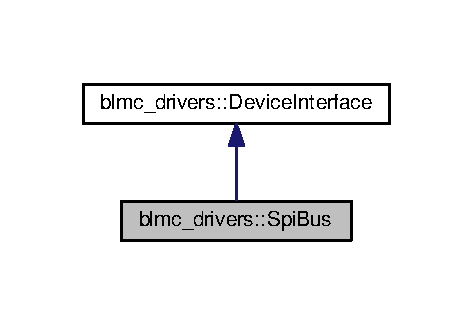
\includegraphics[width=227pt]{classblmc__drivers_1_1SpiBus__inherit__graph}
\end{center}
\end{figure}


Collaboration diagram for blmc\+\_\+drivers\+:\+:Spi\+Bus\+:
\nopagebreak
\begin{figure}[H]
\begin{center}
\leavevmode
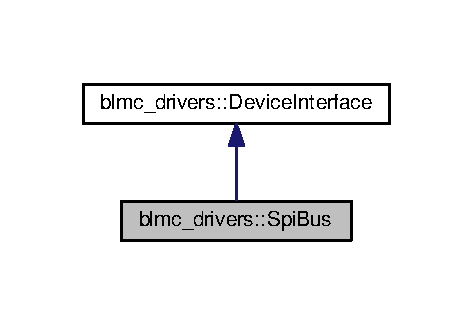
\includegraphics[width=227pt]{classblmc__drivers_1_1SpiBus__coll__graph}
\end{center}
\end{figure}
\subsection*{Public Member Functions}
\begin{DoxyCompactItemize}
\item 
\hyperlink{classblmc__drivers_1_1SpiBus_a020b550fdd3c00a5361f0bee0382dbe2}{Spi\+Bus} (std\+::shared\+\_\+ptr$<$ Master\+Board\+Interface $>$ main\+\_\+board\+\_\+interface, const size\+\_\+t \&nb\+\_\+udrivers, const size\+\_\+t \&history\+\_\+length=1000)
\begin{DoxyCompactList}\small\item\em Construct a new \hyperlink{classblmc__drivers_1_1SpiBus}{Spi\+Bus} object. \end{DoxyCompactList}\item 
\hyperlink{classblmc__drivers_1_1SpiBus_a0c711c24c403c532c5d5bccfa5c1dc68}{$\sim$\+Spi\+Bus} ()
\begin{DoxyCompactList}\small\item\em Destroy the \hyperlink{classblmc__drivers_1_1SpiBus}{Spi\+Bus} object. \end{DoxyCompactList}\item 
virtual std\+::shared\+\_\+ptr$<$ const \hyperlink{classblmc__drivers_1_1MotorInterface_a49b8fc916b9f9debbd7b0988463db5cd}{Motor\+Interface\+::\+Scalar\+Timeseries} $>$ \hyperlink{classblmc__drivers_1_1SpiBus_a57e12fc52e0d499344a7fc858256118e}{get\+\_\+measurement} (const size\+\_\+t udriver\+\_\+id, const \hyperlink{classblmc__drivers_1_1MotorBoardInterface_a8e869cbdb9fcc872ba5a33813e0dfafb}{Motor\+Board\+Interface\+::\+Measurement\+Index} \&index) const 
\begin{DoxyCompactList}\small\item\em Output and status. \end{DoxyCompactList}\item 
virtual std\+::shared\+\_\+ptr$<$ const \hyperlink{classblmc__drivers_1_1MotorBoardInterface_ae3777e484dda60c4abe87f2b542ddfb8}{Motor\+Board\+Interface\+::\+Status\+Timeseries} $>$ \hyperlink{classblmc__drivers_1_1SpiBus_a573b8d5797abaec646a6f14e019f9c24}{get\+\_\+status} (const size\+\_\+t udriver\+\_\+id) const 
\begin{DoxyCompactList}\small\item\em Get the status of the motor board. \end{DoxyCompactList}\item 
virtual std\+::shared\+\_\+ptr$<$ const \hyperlink{classblmc__drivers_1_1MotorInterface_a49b8fc916b9f9debbd7b0988463db5cd}{Motor\+Interface\+::\+Scalar\+Timeseries} $>$ \hyperlink{classblmc__drivers_1_1SpiBus_a237dcb74daf33f6ec7c930573ce4d17d}{get\+\_\+control} (const size\+\_\+t udriver\+\_\+id, const \hyperlink{classblmc__drivers_1_1MotorBoardInterface_a82ed4d0fa527521707281396095a88ca}{Motor\+Board\+Interface\+::\+Control\+Index} \&index) const 
\begin{DoxyCompactList}\small\item\em input logs \end{DoxyCompactList}\item 
virtual std\+::shared\+\_\+ptr$<$ const \hyperlink{classblmc__drivers_1_1MotorBoardInterface_ae2afe94a023d9f08a4c689e9b7660f15}{Motor\+Board\+Interface\+::\+Command\+Timeseries} $>$ \hyperlink{classblmc__drivers_1_1SpiBus_ae6a1f926abf8232f468db4fde35a8f68}{get\+\_\+command} (const size\+\_\+t udriver\+\_\+id) const 
\begin{DoxyCompactList}\small\item\em Get the commands to be send. \end{DoxyCompactList}\item 
virtual std\+::shared\+\_\+ptr$<$ const \hyperlink{classblmc__drivers_1_1MotorInterface_a49b8fc916b9f9debbd7b0988463db5cd}{Motor\+Interface\+::\+Scalar\+Timeseries} $>$ \hyperlink{classblmc__drivers_1_1SpiBus_a7ad1599bdccf5a044b532252951ef774}{get\+\_\+sent\+\_\+control} (const size\+\_\+t udriver\+\_\+id, const \hyperlink{classblmc__drivers_1_1MotorBoardInterface_a82ed4d0fa527521707281396095a88ca}{Motor\+Board\+Interface\+::\+Control\+Index} \&index) const 
\begin{DoxyCompactList}\small\item\em Get the sent controls. \end{DoxyCompactList}\item 
virtual std\+::shared\+\_\+ptr$<$ const \hyperlink{classblmc__drivers_1_1MotorBoardInterface_ae2afe94a023d9f08a4c689e9b7660f15}{Motor\+Board\+Interface\+::\+Command\+Timeseries} $>$ \hyperlink{classblmc__drivers_1_1SpiBus_ad869c7ebcb9c1f028e8ed6afcf20f982}{get\+\_\+sent\+\_\+command} (const size\+\_\+t udriver\+\_\+id) const 
\begin{DoxyCompactList}\small\item\em Get the sent commands. \end{DoxyCompactList}\item 
virtual void \hyperlink{classblmc__drivers_1_1SpiBus_a9cf14c27b226c454795cc1e508ae9a2f}{set\+\_\+control} (const size\+\_\+t udriver\+\_\+id, const double \&control, const \hyperlink{classblmc__drivers_1_1MotorBoardInterface_a82ed4d0fa527521707281396095a88ca}{Motor\+Board\+Interface\+::\+Control\+Index} \&index)
\begin{DoxyCompactList}\small\item\em Setters. \end{DoxyCompactList}\item 
virtual void \hyperlink{classblmc__drivers_1_1SpiBus_af5ca19baccb36befbbc697cdd2e2922c}{set\+\_\+command} (const size\+\_\+t udriver\+\_\+id, const \hyperlink{classblmc__drivers_1_1MotorBoardCommand}{Motor\+Board\+Command} \&command)
\begin{DoxyCompactList}\small\item\em set\+\_\+command save the command internally. \end{DoxyCompactList}\item 
virtual void \hyperlink{classblmc__drivers_1_1SpiBus_ab3802bb10a387b14c7cedc9175823421}{send\+\_\+if\+\_\+input\+\_\+changed} ()
\begin{DoxyCompactList}\small\item\em Actually send the commands and the controls. \end{DoxyCompactList}\item 
bool \hyperlink{classblmc__drivers_1_1SpiBus_ac8c8047626990074b5203ea8010f4570}{is\+\_\+ready} ()\hypertarget{classblmc__drivers_1_1SpiBus_ac8c8047626990074b5203ea8010f4570}{}\label{classblmc__drivers_1_1SpiBus_ac8c8047626990074b5203ea8010f4570}

\begin{DoxyCompactList}\small\item\em return s only once board and motors are ready. \end{DoxyCompactList}\item 
void \hyperlink{classblmc__drivers_1_1SpiBus_a1ff5ba883178951fdd4cc2c5d41d2342}{wait\+\_\+until\+\_\+ready} ()\hypertarget{classblmc__drivers_1_1SpiBus_a1ff5ba883178951fdd4cc2c5d41d2342}{}\label{classblmc__drivers_1_1SpiBus_a1ff5ba883178951fdd4cc2c5d41d2342}

\begin{DoxyCompactList}\small\item\em Wait until the robot is ready. \end{DoxyCompactList}\end{DoxyCompactItemize}
\subsection*{Private Member Functions}
\begin{DoxyCompactItemize}
\item 
void \hyperlink{classblmc__drivers_1_1SpiBus_a21b3790ae435d8845c1a47e31d628cc9}{loop} ()\hypertarget{classblmc__drivers_1_1SpiBus_a21b3790ae435d8845c1a47e31d628cc9}{}\label{classblmc__drivers_1_1SpiBus_a21b3790ae435d8845c1a47e31d628cc9}

\begin{DoxyCompactList}\small\item\em This is the real time thread that streams the data to/from the main board. \end{DoxyCompactList}\item 
void \hyperlink{classblmc__drivers_1_1SpiBus_ad1332260ea455812464723ede9f2c1d1}{send\+\_\+newest\+\_\+command} ()
\begin{DoxyCompactList}\small\item\em Send the newest control stored in the time series. \end{DoxyCompactList}\item 
void \hyperlink{classblmc__drivers_1_1SpiBus_adedb766b0bcc857f3aa53e3468d4c02a}{send\+\_\+newest\+\_\+controls} ()\hypertarget{classblmc__drivers_1_1SpiBus_adedb766b0bcc857f3aa53e3468d4c02a}{}\label{classblmc__drivers_1_1SpiBus_adedb766b0bcc857f3aa53e3468d4c02a}

\begin{DoxyCompactList}\small\item\em Send the newest control stored in the time series. \end{DoxyCompactList}\end{DoxyCompactItemize}
\subsection*{Static Private Member Functions}
\begin{DoxyCompactItemize}
\item 
static T\+H\+R\+E\+A\+D\+\_\+\+F\+U\+N\+C\+T\+I\+O\+N\+\_\+\+R\+E\+T\+U\+R\+N\+\_\+\+T\+Y\+PE \hyperlink{classblmc__drivers_1_1SpiBus_a1838b3861afd142bb5db570841baada1}{loop} (void $\ast$instance\+\_\+pointer)
\begin{DoxyCompactList}\small\item\em Private methods. \end{DoxyCompactList}\end{DoxyCompactItemize}
\subsection*{Private Attributes}
\begin{DoxyCompactItemize}
\item 
std\+::shared\+\_\+ptr$<$ Master\+Board\+Interface $>$ \hyperlink{classblmc__drivers_1_1SpiBus_aa5505729650a363fc5ea2d03c27f0b90}{main\+\_\+board\+\_\+interface\+\_\+}
\begin{DoxyCompactList}\small\item\em Communication related attributes. \end{DoxyCompactList}\item 
size\+\_\+t \hyperlink{classblmc__drivers_1_1SpiBus_ad6f453d80f7c40994d7c2d770e0bcb7a}{nb\+\_\+udrivers\+\_\+}\hypertarget{classblmc__drivers_1_1SpiBus_ad6f453d80f7c40994d7c2d770e0bcb7a}{}\label{classblmc__drivers_1_1SpiBus_ad6f453d80f7c40994d7c2d770e0bcb7a}

\begin{DoxyCompactList}\small\item\em nb\+\_\+udrivers\+\_\+ is the number of the udriver controlled by the main board. \end{DoxyCompactList}\item 
std\+::vector$<$ std\+::shared\+\_\+ptr$<$ \hyperlink{classblmc__drivers_1_1MotorInterface_a49b8fc916b9f9debbd7b0988463db5cd}{Motor\+Interface\+::\+Scalar\+Timeseries} $>$ $>$ \hyperlink{classblmc__drivers_1_1SpiBus_ae3ad20f9cd7e06585b3af84697870cfa}{measurement\+\_\+}
\begin{DoxyCompactList}\small\item\em Outputs. \end{DoxyCompactList}\item 
std\+::vector$<$ std\+::shared\+\_\+ptr$<$ \hyperlink{classblmc__drivers_1_1MotorBoardInterface_ae3777e484dda60c4abe87f2b542ddfb8}{Motor\+Board\+Interface\+::\+Status\+Timeseries} $>$ $>$ \hyperlink{classblmc__drivers_1_1SpiBus_a6a39a07f72d977243eac5346ae4cabba}{status\+\_\+}\hypertarget{classblmc__drivers_1_1SpiBus_a6a39a07f72d977243eac5346ae4cabba}{}\label{classblmc__drivers_1_1SpiBus_a6a39a07f72d977243eac5346ae4cabba}

\begin{DoxyCompactList}\small\item\em This is the status history of the udriver board. \end{DoxyCompactList}\item 
std\+::vector$<$ std\+::shared\+\_\+ptr$<$ \hyperlink{classblmc__drivers_1_1MotorInterface_a49b8fc916b9f9debbd7b0988463db5cd}{Motor\+Interface\+::\+Scalar\+Timeseries} $>$ $>$ \hyperlink{classblmc__drivers_1_1SpiBus_a39d0629b2cb78b7aeae9a4022ca487ed}{control\+\_\+}
\begin{DoxyCompactList}\small\item\em Inputs. \end{DoxyCompactList}\item 
std\+::vector$<$ std\+::shared\+\_\+ptr$<$ \hyperlink{classblmc__drivers_1_1MotorBoardInterface_ae2afe94a023d9f08a4c689e9b7660f15}{Motor\+Board\+Interface\+::\+Command\+Timeseries} $>$ $>$ \hyperlink{classblmc__drivers_1_1SpiBus_a0dadae58644afb41beba8df8f9f09727}{command\+\_\+}\hypertarget{classblmc__drivers_1_1SpiBus_a0dadae58644afb41beba8df8f9f09727}{}\label{classblmc__drivers_1_1SpiBus_a0dadae58644afb41beba8df8f9f09727}

\begin{DoxyCompactList}\small\item\em This is the buffer of the commands to be sent to the card. \end{DoxyCompactList}\item 
size\+\_\+t \hyperlink{classblmc__drivers_1_1SpiBus_a8d0b70b8d02c386d436051a571930c58}{history\+\_\+length\+\_\+}\hypertarget{classblmc__drivers_1_1SpiBus_a8d0b70b8d02c386d436051a571930c58}{}\label{classblmc__drivers_1_1SpiBus_a8d0b70b8d02c386d436051a571930c58}

\begin{DoxyCompactList}\small\item\em history\+\_\+length\+\_\+ is the length of data buffers in number of iteration. \end{DoxyCompactList}\item 
std\+::vector$<$ std\+::shared\+\_\+ptr$<$ \hyperlink{classblmc__drivers_1_1MotorInterface_a49b8fc916b9f9debbd7b0988463db5cd}{Motor\+Interface\+::\+Scalar\+Timeseries} $>$ $>$ \hyperlink{classblmc__drivers_1_1SpiBus_a9c17b8887fc58ca1d5bfb1d5c2fd1e8a}{sent\+\_\+control\+\_\+}
\begin{DoxyCompactList}\small\item\em Log. \end{DoxyCompactList}\item 
std\+::vector$<$ std\+::shared\+\_\+ptr$<$ \hyperlink{classblmc__drivers_1_1MotorBoardInterface_ae2afe94a023d9f08a4c689e9b7660f15}{Motor\+Board\+Interface\+::\+Command\+Timeseries} $>$ $>$ \hyperlink{classblmc__drivers_1_1SpiBus_aa0e964e18db278c1d281d1406ff6d42a}{sent\+\_\+command\+\_\+}\hypertarget{classblmc__drivers_1_1SpiBus_aa0e964e18db278c1d281d1406ff6d42a}{}\label{classblmc__drivers_1_1SpiBus_aa0e964e18db278c1d281d1406ff6d42a}

\begin{DoxyCompactList}\small\item\em This is the history of the already sent commands. \end{DoxyCompactList}\item 
bool \hyperlink{classblmc__drivers_1_1SpiBus_acf6f61ce04098f05fd04971b477da07c}{is\+\_\+loop\+\_\+active\+\_\+}
\begin{DoxyCompactList}\small\item\em Loop management. \end{DoxyCompactList}\item 
bool \hyperlink{classblmc__drivers_1_1SpiBus_ab1ac8ef913898d20cc678f205e27662e}{motors\+\_\+are\+\_\+paused\+\_\+}\hypertarget{classblmc__drivers_1_1SpiBus_ab1ac8ef913898d20cc678f205e27662e}{}\label{classblmc__drivers_1_1SpiBus_ab1ac8ef913898d20cc678f205e27662e}

\begin{DoxyCompactList}\small\item\em Are motor in idle mode = 0 torques. \end{DoxyCompactList}\item 
int \hyperlink{classblmc__drivers_1_1SpiBus_ab861c026ce0d206b802ab521055885fd}{control\+\_\+timeout\+\_\+ms\+\_\+}\hypertarget{classblmc__drivers_1_1SpiBus_ab861c026ce0d206b802ab521055885fd}{}\label{classblmc__drivers_1_1SpiBus_ab861c026ce0d206b802ab521055885fd}

\begin{DoxyCompactList}\small\item\em If no control is sent for more than control\+\_\+timeout\+\_\+ms\+\_\+ the board will shut down. \end{DoxyCompactList}\item 
real\+\_\+time\+\_\+tools\+::\+Real\+Time\+Thread \hyperlink{classblmc__drivers_1_1SpiBus_aaae2fa36dfe60f6155cf8b010c16fc8f}{rt\+\_\+thread\+\_\+}\hypertarget{classblmc__drivers_1_1SpiBus_aaae2fa36dfe60f6155cf8b010c16fc8f}{}\label{classblmc__drivers_1_1SpiBus_aaae2fa36dfe60f6155cf8b010c16fc8f}

\begin{DoxyCompactList}\small\item\em This is the thread object that allow to spwan a real-\/time thread or not dependening on the current OS. \end{DoxyCompactList}\item 
std\+::array$<$ bool, 12 $>$ \hyperlink{classblmc__drivers_1_1SpiBus_a5805dd95171df8f26efdae85ea02662c}{motor\+\_\+index\+\_\+toggle\+\_\+bits\+\_\+}
\begin{DoxyCompactList}\small\item\em Everytime a motor index is detected the corresponding bit change for the opposite value. \end{DoxyCompactList}\end{DoxyCompactItemize}


\subsection{Constructor \& Destructor Documentation}
\index{blmc\+\_\+drivers\+::\+Spi\+Bus@{blmc\+\_\+drivers\+::\+Spi\+Bus}!Spi\+Bus@{Spi\+Bus}}
\index{Spi\+Bus@{Spi\+Bus}!blmc\+\_\+drivers\+::\+Spi\+Bus@{blmc\+\_\+drivers\+::\+Spi\+Bus}}
\subsubsection[{\texorpdfstring{Spi\+Bus(std\+::shared\+\_\+ptr$<$ Master\+Board\+Interface $>$ main\+\_\+board\+\_\+interface, const size\+\_\+t \&nb\+\_\+udrivers, const size\+\_\+t \&history\+\_\+length=1000)}{SpiBus(std::shared_ptr< MasterBoardInterface > main_board_interface, const size_t &nb_udrivers, const size_t &history_length=1000)}}]{\setlength{\rightskip}{0pt plus 5cm}blmc\+\_\+drivers\+::\+Spi\+Bus\+::\+Spi\+Bus (
\begin{DoxyParamCaption}
\item[{std\+::shared\+\_\+ptr$<$ Master\+Board\+Interface $>$}]{main\+\_\+board\+\_\+interface, }
\item[{const size\+\_\+t \&}]{nb\+\_\+udrivers, }
\item[{const size\+\_\+t \&}]{history\+\_\+length = {\ttfamily 1000}}
\end{DoxyParamCaption}
)}\hypertarget{classblmc__drivers_1_1SpiBus_a020b550fdd3c00a5361f0bee0382dbe2}{}\label{classblmc__drivers_1_1SpiBus_a020b550fdd3c00a5361f0bee0382dbe2}


Construct a new \hyperlink{classblmc__drivers_1_1SpiBus}{Spi\+Bus} object. 

The constructor starts a real time thread\+: \hyperlink{classblmc__drivers_1_1SpiBus_a21b3790ae435d8845c1a47e31d628cc9}{Spi\+Bus\+::loop()}. This thread streams the data back and forth collecting the sensor data and sends the control/commands.


\begin{DoxyParams}{Parameters}
{\em main\+\_\+board\+\_\+interface} & is the object that communicate with the main board. The main board provides the hardware informations. \\
\hline
{\em nb\+\_\+udrivers} & is the number udrivers plugged on the main board. \\
\hline
{\em history\+\_\+length} & is the size of the buffer of messages stored. \\
\hline
\end{DoxyParams}
\index{blmc\+\_\+drivers\+::\+Spi\+Bus@{blmc\+\_\+drivers\+::\+Spi\+Bus}!````~Spi\+Bus@{$\sim$\+Spi\+Bus}}
\index{````~Spi\+Bus@{$\sim$\+Spi\+Bus}!blmc\+\_\+drivers\+::\+Spi\+Bus@{blmc\+\_\+drivers\+::\+Spi\+Bus}}
\subsubsection[{\texorpdfstring{$\sim$\+Spi\+Bus()}{~SpiBus()}}]{\setlength{\rightskip}{0pt plus 5cm}blmc\+\_\+drivers\+::\+Spi\+Bus\+::$\sim$\+Spi\+Bus (
\begin{DoxyParamCaption}
{}
\end{DoxyParamCaption}
)}\hypertarget{classblmc__drivers_1_1SpiBus_a0c711c24c403c532c5d5bccfa5c1dc68}{}\label{classblmc__drivers_1_1SpiBus_a0c711c24c403c532c5d5bccfa5c1dc68}


Destroy the \hyperlink{classblmc__drivers_1_1SpiBus}{Spi\+Bus} object. 

The destructor handles the proper shutdown of the class and the threads. 

\subsection{Member Function Documentation}
\index{blmc\+\_\+drivers\+::\+Spi\+Bus@{blmc\+\_\+drivers\+::\+Spi\+Bus}!get\+\_\+command@{get\+\_\+command}}
\index{get\+\_\+command@{get\+\_\+command}!blmc\+\_\+drivers\+::\+Spi\+Bus@{blmc\+\_\+drivers\+::\+Spi\+Bus}}
\subsubsection[{\texorpdfstring{get\+\_\+command(const size\+\_\+t udriver\+\_\+id) const }{get_command(const size_t udriver_id) const }}]{\setlength{\rightskip}{0pt plus 5cm}std\+::shared\+\_\+ptr$<$ const {\bf Motor\+Board\+Interface\+::\+Command\+Timeseries} $>$ blmc\+\_\+drivers\+::\+Spi\+Bus\+::get\+\_\+command (
\begin{DoxyParamCaption}
\item[{const size\+\_\+t}]{udriver\+\_\+id}
\end{DoxyParamCaption}
) const\hspace{0.3cm}{\ttfamily [virtual]}}\hypertarget{classblmc__drivers_1_1SpiBus_ae6a1f926abf8232f468db4fde35a8f68}{}\label{classblmc__drivers_1_1SpiBus_ae6a1f926abf8232f468db4fde35a8f68}


Get the commands to be send. 

\begin{DoxyReturn}{Returns}
Ptr$<$const Command\+Timeseries$>$ is the list of the commands to be send. Inherited from \hyperlink{classblmc__drivers_1_1MotorBoardInterface}{Motor\+Board\+Interface} 
\end{DoxyReturn}
\index{blmc\+\_\+drivers\+::\+Spi\+Bus@{blmc\+\_\+drivers\+::\+Spi\+Bus}!get\+\_\+control@{get\+\_\+control}}
\index{get\+\_\+control@{get\+\_\+control}!blmc\+\_\+drivers\+::\+Spi\+Bus@{blmc\+\_\+drivers\+::\+Spi\+Bus}}
\subsubsection[{\texorpdfstring{get\+\_\+control(const size\+\_\+t udriver\+\_\+id, const Motor\+Board\+Interface\+::\+Control\+Index \&index) const }{get_control(const size_t udriver_id, const MotorBoardInterface::ControlIndex &index) const }}]{\setlength{\rightskip}{0pt plus 5cm}std\+::shared\+\_\+ptr$<$ const {\bf Motor\+Board\+Interface\+::\+Scalar\+Timeseries} $>$ blmc\+\_\+drivers\+::\+Spi\+Bus\+::get\+\_\+control (
\begin{DoxyParamCaption}
\item[{const size\+\_\+t}]{udriver\+\_\+id, }
\item[{const {\bf Motor\+Board\+Interface\+::\+Control\+Index} \&}]{index}
\end{DoxyParamCaption}
) const\hspace{0.3cm}{\ttfamily [virtual]}}\hypertarget{classblmc__drivers_1_1SpiBus_a237dcb74daf33f6ec7c930573ce4d17d}{}\label{classblmc__drivers_1_1SpiBus_a237dcb74daf33f6ec7c930573ce4d17d}


input logs 

input logs Get the controls to be send.


\begin{DoxyParams}{Parameters}
{\em index} & define the kind of control we are looking for. \\
\hline
\end{DoxyParams}
\begin{DoxyReturn}{Returns}
Ptr$<$const Scalar\+Timeseries$>$ is the list of the controls to be send. Inherited from \hyperlink{classblmc__drivers_1_1MotorBoardInterface}{Motor\+Board\+Interface} 
\end{DoxyReturn}
\index{blmc\+\_\+drivers\+::\+Spi\+Bus@{blmc\+\_\+drivers\+::\+Spi\+Bus}!get\+\_\+measurement@{get\+\_\+measurement}}
\index{get\+\_\+measurement@{get\+\_\+measurement}!blmc\+\_\+drivers\+::\+Spi\+Bus@{blmc\+\_\+drivers\+::\+Spi\+Bus}}
\subsubsection[{\texorpdfstring{get\+\_\+measurement(const size\+\_\+t udriver\+\_\+id, const Motor\+Board\+Interface\+::\+Measurement\+Index \&index) const }{get_measurement(const size_t udriver_id, const MotorBoardInterface::MeasurementIndex &index) const }}]{\setlength{\rightskip}{0pt plus 5cm}std\+::shared\+\_\+ptr$<$ const {\bf Motor\+Board\+Interface\+::\+Scalar\+Timeseries} $>$ blmc\+\_\+drivers\+::\+Spi\+Bus\+::get\+\_\+measurement (
\begin{DoxyParamCaption}
\item[{const size\+\_\+t}]{udriver\+\_\+id, }
\item[{const {\bf Motor\+Board\+Interface\+::\+Measurement\+Index} \&}]{index}
\end{DoxyParamCaption}
) const\hspace{0.3cm}{\ttfamily [virtual]}}\hypertarget{classblmc__drivers_1_1SpiBus_a57e12fc52e0d499344a7fc858256118e}{}\label{classblmc__drivers_1_1SpiBus_a57e12fc52e0d499344a7fc858256118e}


Output and status. 

Get the measurements from the main board.


\begin{DoxyParams}{Parameters}
{\em udriver\+\_\+id} & is the index of the spi port on the control board \\
\hline
{\em index} & \\
\hline
\end{DoxyParams}
\begin{DoxyReturn}{Returns}
std\+::shared\+\_\+ptr$<$const Motor\+Interface\+::\+Scalar\+Timeseries$>$ 
\end{DoxyReturn}
\index{blmc\+\_\+drivers\+::\+Spi\+Bus@{blmc\+\_\+drivers\+::\+Spi\+Bus}!get\+\_\+sent\+\_\+command@{get\+\_\+sent\+\_\+command}}
\index{get\+\_\+sent\+\_\+command@{get\+\_\+sent\+\_\+command}!blmc\+\_\+drivers\+::\+Spi\+Bus@{blmc\+\_\+drivers\+::\+Spi\+Bus}}
\subsubsection[{\texorpdfstring{get\+\_\+sent\+\_\+command(const size\+\_\+t udriver\+\_\+id) const }{get_sent_command(const size_t udriver_id) const }}]{\setlength{\rightskip}{0pt plus 5cm}std\+::shared\+\_\+ptr$<$ const {\bf Motor\+Board\+Interface\+::\+Command\+Timeseries} $>$ blmc\+\_\+drivers\+::\+Spi\+Bus\+::get\+\_\+sent\+\_\+command (
\begin{DoxyParamCaption}
\item[{const size\+\_\+t}]{udriver\+\_\+id}
\end{DoxyParamCaption}
) const\hspace{0.3cm}{\ttfamily [virtual]}}\hypertarget{classblmc__drivers_1_1SpiBus_ad869c7ebcb9c1f028e8ed6afcf20f982}{}\label{classblmc__drivers_1_1SpiBus_ad869c7ebcb9c1f028e8ed6afcf20f982}


Get the sent commands. 

\begin{DoxyReturn}{Returns}
Ptr$<$const Command\+Timeseries$>$ is the list of the commands sent recently. Inherited from \hyperlink{classblmc__drivers_1_1MotorBoardInterface}{Motor\+Board\+Interface} 
\end{DoxyReturn}
\index{blmc\+\_\+drivers\+::\+Spi\+Bus@{blmc\+\_\+drivers\+::\+Spi\+Bus}!get\+\_\+sent\+\_\+control@{get\+\_\+sent\+\_\+control}}
\index{get\+\_\+sent\+\_\+control@{get\+\_\+sent\+\_\+control}!blmc\+\_\+drivers\+::\+Spi\+Bus@{blmc\+\_\+drivers\+::\+Spi\+Bus}}
\subsubsection[{\texorpdfstring{get\+\_\+sent\+\_\+control(const size\+\_\+t udriver\+\_\+id, const Motor\+Board\+Interface\+::\+Control\+Index \&index) const }{get_sent_control(const size_t udriver_id, const MotorBoardInterface::ControlIndex &index) const }}]{\setlength{\rightskip}{0pt plus 5cm}std\+::shared\+\_\+ptr$<$ const {\bf Motor\+Board\+Interface\+::\+Scalar\+Timeseries} $>$ blmc\+\_\+drivers\+::\+Spi\+Bus\+::get\+\_\+sent\+\_\+control (
\begin{DoxyParamCaption}
\item[{const size\+\_\+t}]{udriver\+\_\+id, }
\item[{const {\bf Motor\+Board\+Interface\+::\+Control\+Index} \&}]{index}
\end{DoxyParamCaption}
) const\hspace{0.3cm}{\ttfamily [virtual]}}\hypertarget{classblmc__drivers_1_1SpiBus_a7ad1599bdccf5a044b532252951ef774}{}\label{classblmc__drivers_1_1SpiBus_a7ad1599bdccf5a044b532252951ef774}


Get the sent controls. 


\begin{DoxyParams}{Parameters}
{\em index} & define the kind of control we are looking for. \\
\hline
\end{DoxyParams}
\begin{DoxyReturn}{Returns}
Ptr$<$const Scalar\+Timeseries$>$ is the list of the controls sent recently. Inherited from \hyperlink{classblmc__drivers_1_1MotorBoardInterface}{Motor\+Board\+Interface} 
\end{DoxyReturn}
\index{blmc\+\_\+drivers\+::\+Spi\+Bus@{blmc\+\_\+drivers\+::\+Spi\+Bus}!get\+\_\+status@{get\+\_\+status}}
\index{get\+\_\+status@{get\+\_\+status}!blmc\+\_\+drivers\+::\+Spi\+Bus@{blmc\+\_\+drivers\+::\+Spi\+Bus}}
\subsubsection[{\texorpdfstring{get\+\_\+status(const size\+\_\+t udriver\+\_\+id) const }{get_status(const size_t udriver_id) const }}]{\setlength{\rightskip}{0pt plus 5cm}std\+::shared\+\_\+ptr$<$ const {\bf Motor\+Board\+Interface\+::\+Status\+Timeseries} $>$ blmc\+\_\+drivers\+::\+Spi\+Bus\+::get\+\_\+status (
\begin{DoxyParamCaption}
\item[{const size\+\_\+t}]{udriver\+\_\+id}
\end{DoxyParamCaption}
) const\hspace{0.3cm}{\ttfamily [virtual]}}\hypertarget{classblmc__drivers_1_1SpiBus_a573b8d5797abaec646a6f14e019f9c24}{}\label{classblmc__drivers_1_1SpiBus_a573b8d5797abaec646a6f14e019f9c24}


Get the status of the motor board. 

\begin{DoxyReturn}{Returns}
Ptr$<$const Status\+Timeseries$>$ is the list of the last status of the card. Inherited from \hyperlink{classblmc__drivers_1_1MotorBoardInterface}{Motor\+Board\+Interface} 
\end{DoxyReturn}
\index{blmc\+\_\+drivers\+::\+Spi\+Bus@{blmc\+\_\+drivers\+::\+Spi\+Bus}!loop@{loop}}
\index{loop@{loop}!blmc\+\_\+drivers\+::\+Spi\+Bus@{blmc\+\_\+drivers\+::\+Spi\+Bus}}
\subsubsection[{\texorpdfstring{loop(void $\ast$instance\+\_\+pointer)}{loop(void *instance_pointer)}}]{\setlength{\rightskip}{0pt plus 5cm}static T\+H\+R\+E\+A\+D\+\_\+\+F\+U\+N\+C\+T\+I\+O\+N\+\_\+\+R\+E\+T\+U\+R\+N\+\_\+\+T\+Y\+PE blmc\+\_\+drivers\+::\+Spi\+Bus\+::loop (
\begin{DoxyParamCaption}
\item[{void $\ast$}]{instance\+\_\+pointer}
\end{DoxyParamCaption}
)\hspace{0.3cm}{\ttfamily [inline]}, {\ttfamily [static]}, {\ttfamily [private]}}\hypertarget{classblmc__drivers_1_1SpiBus_a1838b3861afd142bb5db570841baada1}{}\label{classblmc__drivers_1_1SpiBus_a1838b3861afd142bb5db570841baada1}


Private methods. 

This is the helper function used for spawning the real time thread.


\begin{DoxyParams}{Parameters}
{\em instance\+\_\+pointer} & is the current object in this case. \\
\hline
\end{DoxyParams}
\begin{DoxyReturn}{Returns}
T\+H\+R\+E\+A\+D\+\_\+\+F\+U\+N\+C\+T\+I\+O\+N\+\_\+\+R\+E\+T\+U\+R\+N\+\_\+\+T\+Y\+PE depends on the current OS. 
\end{DoxyReturn}
\index{blmc\+\_\+drivers\+::\+Spi\+Bus@{blmc\+\_\+drivers\+::\+Spi\+Bus}!send\+\_\+if\+\_\+input\+\_\+changed@{send\+\_\+if\+\_\+input\+\_\+changed}}
\index{send\+\_\+if\+\_\+input\+\_\+changed@{send\+\_\+if\+\_\+input\+\_\+changed}!blmc\+\_\+drivers\+::\+Spi\+Bus@{blmc\+\_\+drivers\+::\+Spi\+Bus}}
\subsubsection[{\texorpdfstring{send\+\_\+if\+\_\+input\+\_\+changed()}{send_if_input_changed()}}]{\setlength{\rightskip}{0pt plus 5cm}void blmc\+\_\+drivers\+::\+Spi\+Bus\+::send\+\_\+if\+\_\+input\+\_\+changed (
\begin{DoxyParamCaption}
{}
\end{DoxyParamCaption}
)\hspace{0.3cm}{\ttfamily [virtual]}}\hypertarget{classblmc__drivers_1_1SpiBus_ab3802bb10a387b14c7cedc9175823421}{}\label{classblmc__drivers_1_1SpiBus_ab3802bb10a387b14c7cedc9175823421}


Actually send the commands and the controls. 

Inherited from \hyperlink{classblmc__drivers_1_1MotorBoardInterface}{Motor\+Board\+Interface}. This particualr instance does not actually check if it is is a new command or control as the full status of the robot is exchange at every tick. \index{blmc\+\_\+drivers\+::\+Spi\+Bus@{blmc\+\_\+drivers\+::\+Spi\+Bus}!send\+\_\+newest\+\_\+command@{send\+\_\+newest\+\_\+command}}
\index{send\+\_\+newest\+\_\+command@{send\+\_\+newest\+\_\+command}!blmc\+\_\+drivers\+::\+Spi\+Bus@{blmc\+\_\+drivers\+::\+Spi\+Bus}}
\subsubsection[{\texorpdfstring{send\+\_\+newest\+\_\+command()}{send_newest_command()}}]{\setlength{\rightskip}{0pt plus 5cm}void blmc\+\_\+drivers\+::\+Spi\+Bus\+::send\+\_\+newest\+\_\+command (
\begin{DoxyParamCaption}
{}
\end{DoxyParamCaption}
)\hspace{0.3cm}{\ttfamily [private]}}\hypertarget{classblmc__drivers_1_1SpiBus_ad1332260ea455812464723ede9f2c1d1}{}\label{classblmc__drivers_1_1SpiBus_ad1332260ea455812464723ede9f2c1d1}


Send the newest control stored in the time series. 

Some of the command are not implemented/will be implemented. A warning is issued upon miss-\/use. \index{blmc\+\_\+drivers\+::\+Spi\+Bus@{blmc\+\_\+drivers\+::\+Spi\+Bus}!set\+\_\+command@{set\+\_\+command}}
\index{set\+\_\+command@{set\+\_\+command}!blmc\+\_\+drivers\+::\+Spi\+Bus@{blmc\+\_\+drivers\+::\+Spi\+Bus}}
\subsubsection[{\texorpdfstring{set\+\_\+command(const size\+\_\+t udriver\+\_\+id, const Motor\+Board\+Command \&command)}{set_command(const size_t udriver_id, const MotorBoardCommand &command)}}]{\setlength{\rightskip}{0pt plus 5cm}void blmc\+\_\+drivers\+::\+Spi\+Bus\+::set\+\_\+command (
\begin{DoxyParamCaption}
\item[{const size\+\_\+t}]{udriver\+\_\+id, }
\item[{const {\bf Motor\+Board\+Command} \&}]{command}
\end{DoxyParamCaption}
)\hspace{0.3cm}{\ttfamily [virtual]}}\hypertarget{classblmc__drivers_1_1SpiBus_af5ca19baccb36befbbc697cdd2e2922c}{}\label{classblmc__drivers_1_1SpiBus_af5ca19baccb36befbbc697cdd2e2922c}


set\+\_\+command save the command internally. 

In order to actaully send the controls to the network please call \char`\"{}send\+\_\+if\+\_\+input\+\_\+changed\char`\"{}


\begin{DoxyParams}{Parameters}
{\em command} & is the command to be sent. Inherited from \hyperlink{classblmc__drivers_1_1MotorBoardInterface}{Motor\+Board\+Interface} \\
\hline
\end{DoxyParams}
\index{blmc\+\_\+drivers\+::\+Spi\+Bus@{blmc\+\_\+drivers\+::\+Spi\+Bus}!set\+\_\+control@{set\+\_\+control}}
\index{set\+\_\+control@{set\+\_\+control}!blmc\+\_\+drivers\+::\+Spi\+Bus@{blmc\+\_\+drivers\+::\+Spi\+Bus}}
\subsubsection[{\texorpdfstring{set\+\_\+control(const size\+\_\+t udriver\+\_\+id, const double \&control, const Motor\+Board\+Interface\+::\+Control\+Index \&index)}{set_control(const size_t udriver_id, const double &control, const MotorBoardInterface::ControlIndex &index)}}]{\setlength{\rightskip}{0pt plus 5cm}void blmc\+\_\+drivers\+::\+Spi\+Bus\+::set\+\_\+control (
\begin{DoxyParamCaption}
\item[{const size\+\_\+t}]{udriver\+\_\+id, }
\item[{const double \&}]{control, }
\item[{const {\bf Motor\+Board\+Interface\+::\+Control\+Index} \&}]{index}
\end{DoxyParamCaption}
)\hspace{0.3cm}{\ttfamily [virtual]}}\hypertarget{classblmc__drivers_1_1SpiBus_a9cf14c27b226c454795cc1e508ae9a2f}{}\label{classblmc__drivers_1_1SpiBus_a9cf14c27b226c454795cc1e508ae9a2f}


Setters. 

Setters. set\+\_\+control save the control internally. In order to actaully send the controls to the network please call \char`\"{}send\+\_\+if\+\_\+input\+\_\+changed\char`\"{}


\begin{DoxyParams}{Parameters}
{\em control} & is the value of the control. \\
\hline
{\em index} & define the kind of control we want to send. Inherited from \hyperlink{classblmc__drivers_1_1MotorBoardInterface}{Motor\+Board\+Interface} \\
\hline
\end{DoxyParams}


\subsection{Member Data Documentation}
\index{blmc\+\_\+drivers\+::\+Spi\+Bus@{blmc\+\_\+drivers\+::\+Spi\+Bus}!control\+\_\+@{control\+\_\+}}
\index{control\+\_\+@{control\+\_\+}!blmc\+\_\+drivers\+::\+Spi\+Bus@{blmc\+\_\+drivers\+::\+Spi\+Bus}}
\subsubsection[{\texorpdfstring{control\+\_\+}{control_}}]{\setlength{\rightskip}{0pt plus 5cm}std\+::vector$<$std\+::shared\+\_\+ptr$<${\bf Motor\+Interface\+::\+Scalar\+Timeseries}$>$ $>$ blmc\+\_\+drivers\+::\+Spi\+Bus\+::control\+\_\+\hspace{0.3cm}{\ttfamily [private]}}\hypertarget{classblmc__drivers_1_1SpiBus_a39d0629b2cb78b7aeae9a4022ca487ed}{}\label{classblmc__drivers_1_1SpiBus_a39d0629b2cb78b7aeae9a4022ca487ed}


Inputs. 

This is the buffer of the controls to be sent to card. \index{blmc\+\_\+drivers\+::\+Spi\+Bus@{blmc\+\_\+drivers\+::\+Spi\+Bus}!is\+\_\+loop\+\_\+active\+\_\+@{is\+\_\+loop\+\_\+active\+\_\+}}
\index{is\+\_\+loop\+\_\+active\+\_\+@{is\+\_\+loop\+\_\+active\+\_\+}!blmc\+\_\+drivers\+::\+Spi\+Bus@{blmc\+\_\+drivers\+::\+Spi\+Bus}}
\subsubsection[{\texorpdfstring{is\+\_\+loop\+\_\+active\+\_\+}{is_loop_active_}}]{\setlength{\rightskip}{0pt plus 5cm}bool blmc\+\_\+drivers\+::\+Spi\+Bus\+::is\+\_\+loop\+\_\+active\+\_\+\hspace{0.3cm}{\ttfamily [private]}}\hypertarget{classblmc__drivers_1_1SpiBus_acf6f61ce04098f05fd04971b477da07c}{}\label{classblmc__drivers_1_1SpiBus_acf6f61ce04098f05fd04971b477da07c}


Loop management. 

This boolean makes sure that the loop is stopped upon destruction of this object. \index{blmc\+\_\+drivers\+::\+Spi\+Bus@{blmc\+\_\+drivers\+::\+Spi\+Bus}!main\+\_\+board\+\_\+interface\+\_\+@{main\+\_\+board\+\_\+interface\+\_\+}}
\index{main\+\_\+board\+\_\+interface\+\_\+@{main\+\_\+board\+\_\+interface\+\_\+}!blmc\+\_\+drivers\+::\+Spi\+Bus@{blmc\+\_\+drivers\+::\+Spi\+Bus}}
\subsubsection[{\texorpdfstring{main\+\_\+board\+\_\+interface\+\_\+}{main_board_interface_}}]{\setlength{\rightskip}{0pt plus 5cm}std\+::shared\+\_\+ptr$<$Master\+Board\+Interface$>$ blmc\+\_\+drivers\+::\+Spi\+Bus\+::main\+\_\+board\+\_\+interface\+\_\+\hspace{0.3cm}{\ttfamily [private]}}\hypertarget{classblmc__drivers_1_1SpiBus_aa5505729650a363fc5ea2d03c27f0b90}{}\label{classblmc__drivers_1_1SpiBus_aa5505729650a363fc5ea2d03c27f0b90}


Communication related attributes. 

Main board interface sdk\+: \href{https://github.com/open-dynamic-robot-initiative/master-board}{\tt https\+://github.\+com/open-\/dynamic-\/robot-\/initiative/master-\/board} \index{blmc\+\_\+drivers\+::\+Spi\+Bus@{blmc\+\_\+drivers\+::\+Spi\+Bus}!measurement\+\_\+@{measurement\+\_\+}}
\index{measurement\+\_\+@{measurement\+\_\+}!blmc\+\_\+drivers\+::\+Spi\+Bus@{blmc\+\_\+drivers\+::\+Spi\+Bus}}
\subsubsection[{\texorpdfstring{measurement\+\_\+}{measurement_}}]{\setlength{\rightskip}{0pt plus 5cm}std\+::vector$<$std\+::shared\+\_\+ptr$<${\bf Motor\+Interface\+::\+Scalar\+Timeseries}$>$ $>$ blmc\+\_\+drivers\+::\+Spi\+Bus\+::measurement\+\_\+\hspace{0.3cm}{\ttfamily [private]}}\hypertarget{classblmc__drivers_1_1SpiBus_ae3ad20f9cd7e06585b3af84697870cfa}{}\label{classblmc__drivers_1_1SpiBus_ae3ad20f9cd7e06585b3af84697870cfa}


Outputs. 

All the measurements acquiered from the C\+AN board. \index{blmc\+\_\+drivers\+::\+Spi\+Bus@{blmc\+\_\+drivers\+::\+Spi\+Bus}!motor\+\_\+index\+\_\+toggle\+\_\+bits\+\_\+@{motor\+\_\+index\+\_\+toggle\+\_\+bits\+\_\+}}
\index{motor\+\_\+index\+\_\+toggle\+\_\+bits\+\_\+@{motor\+\_\+index\+\_\+toggle\+\_\+bits\+\_\+}!blmc\+\_\+drivers\+::\+Spi\+Bus@{blmc\+\_\+drivers\+::\+Spi\+Bus}}
\subsubsection[{\texorpdfstring{motor\+\_\+index\+\_\+toggle\+\_\+bits\+\_\+}{motor_index_toggle_bits_}}]{\setlength{\rightskip}{0pt plus 5cm}std\+::array$<$bool, 12$>$ blmc\+\_\+drivers\+::\+Spi\+Bus\+::motor\+\_\+index\+\_\+toggle\+\_\+bits\+\_\+\hspace{0.3cm}{\ttfamily [private]}}\hypertarget{classblmc__drivers_1_1SpiBus_a5805dd95171df8f26efdae85ea02662c}{}\label{classblmc__drivers_1_1SpiBus_a5805dd95171df8f26efdae85ea02662c}


Everytime a motor index is detected the corresponding bit change for the opposite value. 


\begin{DoxyCode}
\textcolor{keywordflow}{if} (index detected on motor X)
\{
    \hyperlink{classblmc__drivers_1_1SpiBus_a5805dd95171df8f26efdae85ea02662c}{motor\_index\_toggle\_bits\_}[X] = !
      \hyperlink{classblmc__drivers_1_1SpiBus_a5805dd95171df8f26efdae85ea02662c}{motor\_index\_toggle\_bits\_}[X]
\}
\end{DoxyCode}
 \index{blmc\+\_\+drivers\+::\+Spi\+Bus@{blmc\+\_\+drivers\+::\+Spi\+Bus}!sent\+\_\+control\+\_\+@{sent\+\_\+control\+\_\+}}
\index{sent\+\_\+control\+\_\+@{sent\+\_\+control\+\_\+}!blmc\+\_\+drivers\+::\+Spi\+Bus@{blmc\+\_\+drivers\+::\+Spi\+Bus}}
\subsubsection[{\texorpdfstring{sent\+\_\+control\+\_\+}{sent_control_}}]{\setlength{\rightskip}{0pt plus 5cm}std\+::vector$<$std\+::shared\+\_\+ptr$<${\bf Motor\+Interface\+::\+Scalar\+Timeseries}$>$ $>$ blmc\+\_\+drivers\+::\+Spi\+Bus\+::sent\+\_\+control\+\_\+\hspace{0.3cm}{\ttfamily [private]}}\hypertarget{classblmc__drivers_1_1SpiBus_a9c17b8887fc58ca1d5bfb1d5c2fd1e8a}{}\label{classblmc__drivers_1_1SpiBus_a9c17b8887fc58ca1d5bfb1d5c2fd1e8a}


Log. 

This is the history of the already sent controls. 

The documentation for this class was generated from the following files\+:\begin{DoxyCompactItemize}
\item 
include/blmc\+\_\+drivers/devices/\hyperlink{spi__bus_8hpp}{spi\+\_\+bus.\+hpp}\item 
src/\hyperlink{spi__bus_8cpp}{spi\+\_\+bus.\+cpp}\end{DoxyCompactItemize}

\hypertarget{classblmc__drivers_1_1SpiMotorBoard}{}\section{blmc\+\_\+drivers\+:\+:Spi\+Motor\+Board Class Reference}
\label{classblmc__drivers_1_1SpiMotorBoard}\index{blmc\+\_\+drivers\+::\+Spi\+Motor\+Board@{blmc\+\_\+drivers\+::\+Spi\+Motor\+Board}}


Inheritance diagram for blmc\+\_\+drivers\+:\+:Spi\+Motor\+Board\+:
\nopagebreak
\begin{figure}[H]
\begin{center}
\leavevmode
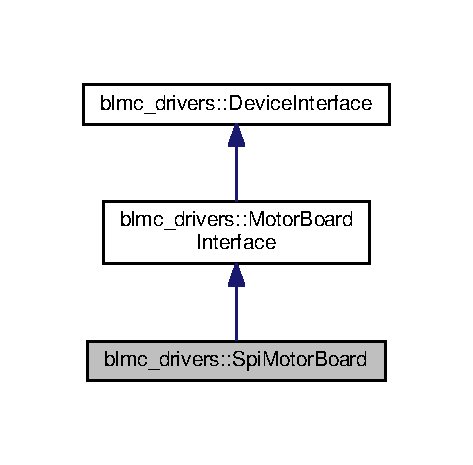
\includegraphics[width=227pt]{classblmc__drivers_1_1SpiMotorBoard__inherit__graph}
\end{center}
\end{figure}


Collaboration diagram for blmc\+\_\+drivers\+:\+:Spi\+Motor\+Board\+:
\nopagebreak
\begin{figure}[H]
\begin{center}
\leavevmode
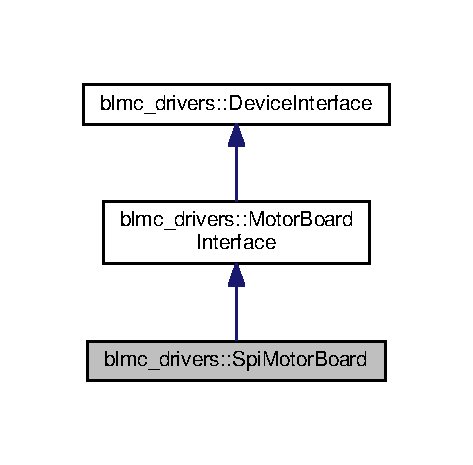
\includegraphics[width=227pt]{classblmc__drivers_1_1SpiMotorBoard__coll__graph}
\end{center}
\end{figure}
\subsection*{Public Member Functions}
\begin{DoxyCompactItemize}
\item 
\hyperlink{classblmc__drivers_1_1SpiMotorBoard_a740572d586d73b678a177bc3de351f8b}{Spi\+Motor\+Board} (std\+::shared\+\_\+ptr$<$ \hyperlink{classblmc__drivers_1_1SpiBus}{Spi\+Bus} $>$ spi\+\_\+bus, const size\+\_\+t udriver\+\_\+id)
\begin{DoxyCompactList}\small\item\em Construct a new \hyperlink{classblmc__drivers_1_1SpiMotorBoard}{Spi\+Motor\+Board} object. \end{DoxyCompactList}\item 
\hyperlink{classblmc__drivers_1_1SpiMotorBoard_a3bc0c19b79504a96426646090c7fbc54}{$\sim$\+Spi\+Motor\+Board} ()
\begin{DoxyCompactList}\small\item\em Destroy the \hyperlink{classblmc__drivers_1_1SpiMotorBoard}{Spi\+Motor\+Board} object. \end{DoxyCompactList}\item 
virtual std\+::shared\+\_\+ptr$<$ const \hyperlink{classblmc__drivers_1_1MotorInterface_a49b8fc916b9f9debbd7b0988463db5cd}{Motor\+Interface\+::\+Scalar\+Timeseries} $>$ \hyperlink{classblmc__drivers_1_1SpiMotorBoard_ae0979b63fe72f5717a156fe670df6b32}{get\+\_\+measurement} (const int \&index) const 
\begin{DoxyCompactList}\small\item\em Output and status. \end{DoxyCompactList}\item 
virtual std\+::shared\+\_\+ptr$<$ const \hyperlink{classblmc__drivers_1_1MotorBoardInterface_ae3777e484dda60c4abe87f2b542ddfb8}{Motor\+Board\+Interface\+::\+Status\+Timeseries} $>$ \hyperlink{classblmc__drivers_1_1SpiMotorBoard_a74e1b0e71721f72769870b7c857f6d92}{get\+\_\+status} () const 
\begin{DoxyCompactList}\small\item\em Get the status of the motor board. \end{DoxyCompactList}\item 
virtual std\+::shared\+\_\+ptr$<$ const \hyperlink{classblmc__drivers_1_1MotorInterface_a49b8fc916b9f9debbd7b0988463db5cd}{Motor\+Interface\+::\+Scalar\+Timeseries} $>$ \hyperlink{classblmc__drivers_1_1SpiMotorBoard_a1b145982a241e234118269c7eeea8d42}{get\+\_\+control} (const int \&index) const 
\begin{DoxyCompactList}\small\item\em input logs \end{DoxyCompactList}\item 
virtual std\+::shared\+\_\+ptr$<$ const \hyperlink{classblmc__drivers_1_1MotorBoardInterface_ae2afe94a023d9f08a4c689e9b7660f15}{Motor\+Board\+Interface\+::\+Command\+Timeseries} $>$ \hyperlink{classblmc__drivers_1_1SpiMotorBoard_a3a3b3b043762c2a232d7e724aea8a6ff}{get\+\_\+command} () const 
\begin{DoxyCompactList}\small\item\em Get the commands to be send. \end{DoxyCompactList}\item 
virtual std\+::shared\+\_\+ptr$<$ const \hyperlink{classblmc__drivers_1_1MotorInterface_a49b8fc916b9f9debbd7b0988463db5cd}{Motor\+Interface\+::\+Scalar\+Timeseries} $>$ \hyperlink{classblmc__drivers_1_1SpiMotorBoard_a26b6e07529dfdbae891a61d6823e3bdb}{get\+\_\+sent\+\_\+control} (const int \&index) const 
\begin{DoxyCompactList}\small\item\em Get the sent controls. \end{DoxyCompactList}\item 
virtual std\+::shared\+\_\+ptr$<$ const \hyperlink{classblmc__drivers_1_1MotorBoardInterface_ae2afe94a023d9f08a4c689e9b7660f15}{Motor\+Board\+Interface\+::\+Command\+Timeseries} $>$ \hyperlink{classblmc__drivers_1_1SpiMotorBoard_a187c15b804f4e7b49f2cd21625ae2512}{get\+\_\+sent\+\_\+command} () const 
\begin{DoxyCompactList}\small\item\em Get the sent commands. \end{DoxyCompactList}\item 
virtual void \hyperlink{classblmc__drivers_1_1SpiMotorBoard_ae11c5382665adfa718bcc43ec1e84b6e}{set\+\_\+control} (const double \&control, const int \&index)
\begin{DoxyCompactList}\small\item\em Setters. \end{DoxyCompactList}\item 
virtual void \hyperlink{classblmc__drivers_1_1SpiMotorBoard_a6b626225af993444bdee397952281772}{set\+\_\+command} (const \hyperlink{classblmc__drivers_1_1MotorBoardCommand}{Motor\+Board\+Command} \&command)
\begin{DoxyCompactList}\small\item\em set\+\_\+command save the command internally. \end{DoxyCompactList}\item 
virtual void \hyperlink{classblmc__drivers_1_1SpiMotorBoard_a39e986b4df42867f8d5896c35c7c4464}{send\+\_\+if\+\_\+input\+\_\+changed} ()
\begin{DoxyCompactList}\small\item\em Actually send the commands and the controls. \end{DoxyCompactList}\item 
bool \hyperlink{classblmc__drivers_1_1SpiMotorBoard_aebd1424f4bee236b2e2ca3bbb1dd8f93}{is\+\_\+ready} ()\hypertarget{classblmc__drivers_1_1SpiMotorBoard_aebd1424f4bee236b2e2ca3bbb1dd8f93}{}\label{classblmc__drivers_1_1SpiMotorBoard_aebd1424f4bee236b2e2ca3bbb1dd8f93}

\begin{DoxyCompactList}\small\item\em return s only once board and motors are ready. \end{DoxyCompactList}\end{DoxyCompactItemize}
\subsection*{Private Attributes}
\begin{DoxyCompactItemize}
\item 
std\+::shared\+\_\+ptr$<$ \hyperlink{classblmc__drivers_1_1SpiBus}{Spi\+Bus} $>$ \hyperlink{classblmc__drivers_1_1SpiMotorBoard_a767abb6f687ed8bf7fef873ab892eaf7}{spi\+\_\+bus\+\_\+}
\begin{DoxyCompactList}\small\item\em Communication related attributes. \end{DoxyCompactList}\item 
size\+\_\+t \hyperlink{classblmc__drivers_1_1SpiMotorBoard_a4b865479722dbecec8ebb66d6b93ecae}{udriver\+\_\+id\+\_\+}
\begin{DoxyCompactList}\small\item\em udriver\+\_\+id\+\_\+ is the index of the udriver controlled by the master board. \end{DoxyCompactList}\end{DoxyCompactItemize}
\subsection*{Additional Inherited Members}


\subsection{Constructor \& Destructor Documentation}
\index{blmc\+\_\+drivers\+::\+Spi\+Motor\+Board@{blmc\+\_\+drivers\+::\+Spi\+Motor\+Board}!Spi\+Motor\+Board@{Spi\+Motor\+Board}}
\index{Spi\+Motor\+Board@{Spi\+Motor\+Board}!blmc\+\_\+drivers\+::\+Spi\+Motor\+Board@{blmc\+\_\+drivers\+::\+Spi\+Motor\+Board}}
\subsubsection[{\texorpdfstring{Spi\+Motor\+Board(std\+::shared\+\_\+ptr$<$ Spi\+Bus $>$ spi\+\_\+bus, const size\+\_\+t udriver\+\_\+id)}{SpiMotorBoard(std::shared_ptr< SpiBus > spi_bus, const size_t udriver_id)}}]{\setlength{\rightskip}{0pt plus 5cm}blmc\+\_\+drivers\+::\+Spi\+Motor\+Board\+::\+Spi\+Motor\+Board (
\begin{DoxyParamCaption}
\item[{std\+::shared\+\_\+ptr$<$ {\bf Spi\+Bus} $>$}]{spi\+\_\+bus, }
\item[{const size\+\_\+t}]{udriver\+\_\+id}
\end{DoxyParamCaption}
)}\hypertarget{classblmc__drivers_1_1SpiMotorBoard_a740572d586d73b678a177bc3de351f8b}{}\label{classblmc__drivers_1_1SpiMotorBoard_a740572d586d73b678a177bc3de351f8b}


Construct a new \hyperlink{classblmc__drivers_1_1SpiMotorBoard}{Spi\+Motor\+Board} object. 

The constructor starts a real time thread\+: Spi\+Motor\+Board\+::loop(). This thread streams the data back and forth collecting the sensor data and sends the control/commands.


\begin{DoxyParams}{Parameters}
{\em spi\+\_\+bus} & is the object that communicate with the master board which in turn communicate with the motor boards. The master board provides the hardware informations and sends the commands. \\
\hline
{\em udriver\+\_\+id} & is the id of the udriver this class represents. \\
\hline
\end{DoxyParams}
\index{blmc\+\_\+drivers\+::\+Spi\+Motor\+Board@{blmc\+\_\+drivers\+::\+Spi\+Motor\+Board}!````~Spi\+Motor\+Board@{$\sim$\+Spi\+Motor\+Board}}
\index{````~Spi\+Motor\+Board@{$\sim$\+Spi\+Motor\+Board}!blmc\+\_\+drivers\+::\+Spi\+Motor\+Board@{blmc\+\_\+drivers\+::\+Spi\+Motor\+Board}}
\subsubsection[{\texorpdfstring{$\sim$\+Spi\+Motor\+Board()}{~SpiMotorBoard()}}]{\setlength{\rightskip}{0pt plus 5cm}blmc\+\_\+drivers\+::\+Spi\+Motor\+Board\+::$\sim$\+Spi\+Motor\+Board (
\begin{DoxyParamCaption}
{}
\end{DoxyParamCaption}
)}\hypertarget{classblmc__drivers_1_1SpiMotorBoard_a3bc0c19b79504a96426646090c7fbc54}{}\label{classblmc__drivers_1_1SpiMotorBoard_a3bc0c19b79504a96426646090c7fbc54}


Destroy the \hyperlink{classblmc__drivers_1_1SpiMotorBoard}{Spi\+Motor\+Board} object. 

The destructor handles the proper shutdown of the class and the threads. 

\subsection{Member Function Documentation}
\index{blmc\+\_\+drivers\+::\+Spi\+Motor\+Board@{blmc\+\_\+drivers\+::\+Spi\+Motor\+Board}!get\+\_\+command@{get\+\_\+command}}
\index{get\+\_\+command@{get\+\_\+command}!blmc\+\_\+drivers\+::\+Spi\+Motor\+Board@{blmc\+\_\+drivers\+::\+Spi\+Motor\+Board}}
\subsubsection[{\texorpdfstring{get\+\_\+command() const }{get_command() const }}]{\setlength{\rightskip}{0pt plus 5cm}std\+::shared\+\_\+ptr$<$ const {\bf Motor\+Board\+Interface\+::\+Command\+Timeseries} $>$ blmc\+\_\+drivers\+::\+Spi\+Motor\+Board\+::get\+\_\+command (
\begin{DoxyParamCaption}
{}
\end{DoxyParamCaption}
) const\hspace{0.3cm}{\ttfamily [virtual]}}\hypertarget{classblmc__drivers_1_1SpiMotorBoard_a3a3b3b043762c2a232d7e724aea8a6ff}{}\label{classblmc__drivers_1_1SpiMotorBoard_a3a3b3b043762c2a232d7e724aea8a6ff}


Get the commands to be send. 

\begin{DoxyReturn}{Returns}
Ptr$<$const Command\+Timeseries$>$ is the list of the commands to be send. Inherited from \hyperlink{classblmc__drivers_1_1MotorBoardInterface}{Motor\+Board\+Interface} 
\end{DoxyReturn}


Implements \hyperlink{classblmc__drivers_1_1MotorBoardInterface_a4913308c1eacc98475aeb8647447c997}{blmc\+\_\+drivers\+::\+Motor\+Board\+Interface}.

\index{blmc\+\_\+drivers\+::\+Spi\+Motor\+Board@{blmc\+\_\+drivers\+::\+Spi\+Motor\+Board}!get\+\_\+control@{get\+\_\+control}}
\index{get\+\_\+control@{get\+\_\+control}!blmc\+\_\+drivers\+::\+Spi\+Motor\+Board@{blmc\+\_\+drivers\+::\+Spi\+Motor\+Board}}
\subsubsection[{\texorpdfstring{get\+\_\+control(const int \&index) const }{get_control(const int &index) const }}]{\setlength{\rightskip}{0pt plus 5cm}std\+::shared\+\_\+ptr$<$ const {\bf Motor\+Board\+Interface\+::\+Scalar\+Timeseries} $>$ blmc\+\_\+drivers\+::\+Spi\+Motor\+Board\+::get\+\_\+control (
\begin{DoxyParamCaption}
\item[{const int \&}]{index}
\end{DoxyParamCaption}
) const\hspace{0.3cm}{\ttfamily [virtual]}}\hypertarget{classblmc__drivers_1_1SpiMotorBoard_a1b145982a241e234118269c7eeea8d42}{}\label{classblmc__drivers_1_1SpiMotorBoard_a1b145982a241e234118269c7eeea8d42}


input logs 

input logs Get the controls to be send.


\begin{DoxyParams}{Parameters}
{\em index} & define the kind of control we are looking for. \\
\hline
\end{DoxyParams}
\begin{DoxyReturn}{Returns}
Ptr$<$const Scalar\+Timeseries$>$ is the list of the controls to be send. Inherited from \hyperlink{classblmc__drivers_1_1MotorBoardInterface}{Motor\+Board\+Interface} 
\end{DoxyReturn}


Implements \hyperlink{classblmc__drivers_1_1MotorBoardInterface_aa5eeed12c851993f2e2c93f5479df9de}{blmc\+\_\+drivers\+::\+Motor\+Board\+Interface}.

\index{blmc\+\_\+drivers\+::\+Spi\+Motor\+Board@{blmc\+\_\+drivers\+::\+Spi\+Motor\+Board}!get\+\_\+measurement@{get\+\_\+measurement}}
\index{get\+\_\+measurement@{get\+\_\+measurement}!blmc\+\_\+drivers\+::\+Spi\+Motor\+Board@{blmc\+\_\+drivers\+::\+Spi\+Motor\+Board}}
\subsubsection[{\texorpdfstring{get\+\_\+measurement(const int \&index) const }{get_measurement(const int &index) const }}]{\setlength{\rightskip}{0pt plus 5cm}std\+::shared\+\_\+ptr$<$ const {\bf Motor\+Board\+Interface\+::\+Scalar\+Timeseries} $>$ blmc\+\_\+drivers\+::\+Spi\+Motor\+Board\+::get\+\_\+measurement (
\begin{DoxyParamCaption}
\item[{const int \&}]{index}
\end{DoxyParamCaption}
) const\hspace{0.3cm}{\ttfamily [virtual]}}\hypertarget{classblmc__drivers_1_1SpiMotorBoard_ae0979b63fe72f5717a156fe670df6b32}{}\label{classblmc__drivers_1_1SpiMotorBoard_ae0979b63fe72f5717a156fe670df6b32}


Output and status. 

Getters. Get the measurements


\begin{DoxyParams}{Parameters}
{\em index} & is the kind of measurement we are looking for. \\
\hline
\end{DoxyParams}
\begin{DoxyReturn}{Returns}
Ptr$<$const Scalar\+Timeseries$>$ is the list of the last time stamped measurement acquiered. Inherited from \hyperlink{classblmc__drivers_1_1MotorBoardInterface}{Motor\+Board\+Interface} 
\end{DoxyReturn}


Implements \hyperlink{classblmc__drivers_1_1MotorBoardInterface_a34828a0375a3bd1fede4deb4fc74c04d}{blmc\+\_\+drivers\+::\+Motor\+Board\+Interface}.

\index{blmc\+\_\+drivers\+::\+Spi\+Motor\+Board@{blmc\+\_\+drivers\+::\+Spi\+Motor\+Board}!get\+\_\+sent\+\_\+command@{get\+\_\+sent\+\_\+command}}
\index{get\+\_\+sent\+\_\+command@{get\+\_\+sent\+\_\+command}!blmc\+\_\+drivers\+::\+Spi\+Motor\+Board@{blmc\+\_\+drivers\+::\+Spi\+Motor\+Board}}
\subsubsection[{\texorpdfstring{get\+\_\+sent\+\_\+command() const }{get_sent_command() const }}]{\setlength{\rightskip}{0pt plus 5cm}std\+::shared\+\_\+ptr$<$ const {\bf Motor\+Board\+Interface\+::\+Command\+Timeseries} $>$ blmc\+\_\+drivers\+::\+Spi\+Motor\+Board\+::get\+\_\+sent\+\_\+command (
\begin{DoxyParamCaption}
{}
\end{DoxyParamCaption}
) const\hspace{0.3cm}{\ttfamily [virtual]}}\hypertarget{classblmc__drivers_1_1SpiMotorBoard_a187c15b804f4e7b49f2cd21625ae2512}{}\label{classblmc__drivers_1_1SpiMotorBoard_a187c15b804f4e7b49f2cd21625ae2512}


Get the sent commands. 

\begin{DoxyReturn}{Returns}
Ptr$<$const Command\+Timeseries$>$ is the list of the commands sent recently. Inherited from \hyperlink{classblmc__drivers_1_1MotorBoardInterface}{Motor\+Board\+Interface} 
\end{DoxyReturn}


Implements \hyperlink{classblmc__drivers_1_1MotorBoardInterface_afd3de58f7a900347154b8d323f1c1d94}{blmc\+\_\+drivers\+::\+Motor\+Board\+Interface}.

\index{blmc\+\_\+drivers\+::\+Spi\+Motor\+Board@{blmc\+\_\+drivers\+::\+Spi\+Motor\+Board}!get\+\_\+sent\+\_\+control@{get\+\_\+sent\+\_\+control}}
\index{get\+\_\+sent\+\_\+control@{get\+\_\+sent\+\_\+control}!blmc\+\_\+drivers\+::\+Spi\+Motor\+Board@{blmc\+\_\+drivers\+::\+Spi\+Motor\+Board}}
\subsubsection[{\texorpdfstring{get\+\_\+sent\+\_\+control(const int \&index) const }{get_sent_control(const int &index) const }}]{\setlength{\rightskip}{0pt plus 5cm}std\+::shared\+\_\+ptr$<$ const {\bf Motor\+Board\+Interface\+::\+Scalar\+Timeseries} $>$ blmc\+\_\+drivers\+::\+Spi\+Motor\+Board\+::get\+\_\+sent\+\_\+control (
\begin{DoxyParamCaption}
\item[{const int \&}]{index}
\end{DoxyParamCaption}
) const\hspace{0.3cm}{\ttfamily [virtual]}}\hypertarget{classblmc__drivers_1_1SpiMotorBoard_a26b6e07529dfdbae891a61d6823e3bdb}{}\label{classblmc__drivers_1_1SpiMotorBoard_a26b6e07529dfdbae891a61d6823e3bdb}


Get the sent controls. 


\begin{DoxyParams}{Parameters}
{\em index} & define the kind of control we are looking for. \\
\hline
\end{DoxyParams}
\begin{DoxyReturn}{Returns}
Ptr$<$const Scalar\+Timeseries$>$ is the list of the controls sent recently. Inherited from \hyperlink{classblmc__drivers_1_1MotorBoardInterface}{Motor\+Board\+Interface} 
\end{DoxyReturn}


Implements \hyperlink{classblmc__drivers_1_1MotorBoardInterface_a8dc6222e915fc96d89b13cbb0fcb0cda}{blmc\+\_\+drivers\+::\+Motor\+Board\+Interface}.

\index{blmc\+\_\+drivers\+::\+Spi\+Motor\+Board@{blmc\+\_\+drivers\+::\+Spi\+Motor\+Board}!get\+\_\+status@{get\+\_\+status}}
\index{get\+\_\+status@{get\+\_\+status}!blmc\+\_\+drivers\+::\+Spi\+Motor\+Board@{blmc\+\_\+drivers\+::\+Spi\+Motor\+Board}}
\subsubsection[{\texorpdfstring{get\+\_\+status() const }{get_status() const }}]{\setlength{\rightskip}{0pt plus 5cm}std\+::shared\+\_\+ptr$<$ const {\bf Motor\+Board\+Interface\+::\+Status\+Timeseries} $>$ blmc\+\_\+drivers\+::\+Spi\+Motor\+Board\+::get\+\_\+status (
\begin{DoxyParamCaption}
{}
\end{DoxyParamCaption}
) const\hspace{0.3cm}{\ttfamily [virtual]}}\hypertarget{classblmc__drivers_1_1SpiMotorBoard_a74e1b0e71721f72769870b7c857f6d92}{}\label{classblmc__drivers_1_1SpiMotorBoard_a74e1b0e71721f72769870b7c857f6d92}


Get the status of the motor board. 

\begin{DoxyReturn}{Returns}
Ptr$<$const Status\+Timeseries$>$ is the list of the last status of the card. Inherited from \hyperlink{classblmc__drivers_1_1MotorBoardInterface}{Motor\+Board\+Interface} 
\end{DoxyReturn}


Implements \hyperlink{classblmc__drivers_1_1MotorBoardInterface_a13b1ffa7d10c1c753d76eaf5368714e3}{blmc\+\_\+drivers\+::\+Motor\+Board\+Interface}.

\index{blmc\+\_\+drivers\+::\+Spi\+Motor\+Board@{blmc\+\_\+drivers\+::\+Spi\+Motor\+Board}!send\+\_\+if\+\_\+input\+\_\+changed@{send\+\_\+if\+\_\+input\+\_\+changed}}
\index{send\+\_\+if\+\_\+input\+\_\+changed@{send\+\_\+if\+\_\+input\+\_\+changed}!blmc\+\_\+drivers\+::\+Spi\+Motor\+Board@{blmc\+\_\+drivers\+::\+Spi\+Motor\+Board}}
\subsubsection[{\texorpdfstring{send\+\_\+if\+\_\+input\+\_\+changed()}{send_if_input_changed()}}]{\setlength{\rightskip}{0pt plus 5cm}void blmc\+\_\+drivers\+::\+Spi\+Motor\+Board\+::send\+\_\+if\+\_\+input\+\_\+changed (
\begin{DoxyParamCaption}
{}
\end{DoxyParamCaption}
)\hspace{0.3cm}{\ttfamily [virtual]}}\hypertarget{classblmc__drivers_1_1SpiMotorBoard_a39e986b4df42867f8d5896c35c7c4464}{}\label{classblmc__drivers_1_1SpiMotorBoard_a39e986b4df42867f8d5896c35c7c4464}


Actually send the commands and the controls. 

Inherited from \hyperlink{classblmc__drivers_1_1MotorBoardInterface}{Motor\+Board\+Interface}. This particualr instance does not actually check if it is is a new command or control as the full status of the robot is exchange at every tick. 

Implements \hyperlink{classblmc__drivers_1_1MotorBoardInterface_a79afd172c736718868f4d269125f2581}{blmc\+\_\+drivers\+::\+Motor\+Board\+Interface}.

\index{blmc\+\_\+drivers\+::\+Spi\+Motor\+Board@{blmc\+\_\+drivers\+::\+Spi\+Motor\+Board}!set\+\_\+command@{set\+\_\+command}}
\index{set\+\_\+command@{set\+\_\+command}!blmc\+\_\+drivers\+::\+Spi\+Motor\+Board@{blmc\+\_\+drivers\+::\+Spi\+Motor\+Board}}
\subsubsection[{\texorpdfstring{set\+\_\+command(const Motor\+Board\+Command \&command)}{set_command(const MotorBoardCommand &command)}}]{\setlength{\rightskip}{0pt plus 5cm}void blmc\+\_\+drivers\+::\+Spi\+Motor\+Board\+::set\+\_\+command (
\begin{DoxyParamCaption}
\item[{const {\bf Motor\+Board\+Command} \&}]{command}
\end{DoxyParamCaption}
)\hspace{0.3cm}{\ttfamily [virtual]}}\hypertarget{classblmc__drivers_1_1SpiMotorBoard_a6b626225af993444bdee397952281772}{}\label{classblmc__drivers_1_1SpiMotorBoard_a6b626225af993444bdee397952281772}


set\+\_\+command save the command internally. 

In order to actaully send the controls to the network please call \char`\"{}send\+\_\+if\+\_\+input\+\_\+changed\char`\"{}


\begin{DoxyParams}{Parameters}
{\em command} & is the command to be sent. Inherited from \hyperlink{classblmc__drivers_1_1MotorBoardInterface}{Motor\+Board\+Interface} \\
\hline
\end{DoxyParams}


Implements \hyperlink{classblmc__drivers_1_1MotorBoardInterface_a86b4ff810ca652d6761090ceaff65621}{blmc\+\_\+drivers\+::\+Motor\+Board\+Interface}.

\index{blmc\+\_\+drivers\+::\+Spi\+Motor\+Board@{blmc\+\_\+drivers\+::\+Spi\+Motor\+Board}!set\+\_\+control@{set\+\_\+control}}
\index{set\+\_\+control@{set\+\_\+control}!blmc\+\_\+drivers\+::\+Spi\+Motor\+Board@{blmc\+\_\+drivers\+::\+Spi\+Motor\+Board}}
\subsubsection[{\texorpdfstring{set\+\_\+control(const double \&control, const int \&index)}{set_control(const double &control, const int &index)}}]{\setlength{\rightskip}{0pt plus 5cm}void blmc\+\_\+drivers\+::\+Spi\+Motor\+Board\+::set\+\_\+control (
\begin{DoxyParamCaption}
\item[{const double \&}]{control, }
\item[{const int \&}]{index}
\end{DoxyParamCaption}
)\hspace{0.3cm}{\ttfamily [virtual]}}\hypertarget{classblmc__drivers_1_1SpiMotorBoard_ae11c5382665adfa718bcc43ec1e84b6e}{}\label{classblmc__drivers_1_1SpiMotorBoard_ae11c5382665adfa718bcc43ec1e84b6e}


Setters. 

Setters. set\+\_\+control save the control internally. In order to actaully send the controls to the network please call \char`\"{}send\+\_\+if\+\_\+input\+\_\+changed\char`\"{}


\begin{DoxyParams}{Parameters}
{\em control} & is the value of the control. \\
\hline
{\em index} & define the kind of control we want to send. Inherited from \hyperlink{classblmc__drivers_1_1MotorBoardInterface}{Motor\+Board\+Interface} \\
\hline
\end{DoxyParams}


Implements \hyperlink{classblmc__drivers_1_1MotorBoardInterface_a3ace57ba3e09b9b3120d09303ff39a61}{blmc\+\_\+drivers\+::\+Motor\+Board\+Interface}.



\subsection{Member Data Documentation}
\index{blmc\+\_\+drivers\+::\+Spi\+Motor\+Board@{blmc\+\_\+drivers\+::\+Spi\+Motor\+Board}!spi\+\_\+bus\+\_\+@{spi\+\_\+bus\+\_\+}}
\index{spi\+\_\+bus\+\_\+@{spi\+\_\+bus\+\_\+}!blmc\+\_\+drivers\+::\+Spi\+Motor\+Board@{blmc\+\_\+drivers\+::\+Spi\+Motor\+Board}}
\subsubsection[{\texorpdfstring{spi\+\_\+bus\+\_\+}{spi_bus_}}]{\setlength{\rightskip}{0pt plus 5cm}std\+::shared\+\_\+ptr$<${\bf Spi\+Bus}$>$ blmc\+\_\+drivers\+::\+Spi\+Motor\+Board\+::spi\+\_\+bus\+\_\+\hspace{0.3cm}{\ttfamily [private]}}\hypertarget{classblmc__drivers_1_1SpiMotorBoard_a767abb6f687ed8bf7fef873ab892eaf7}{}\label{classblmc__drivers_1_1SpiMotorBoard_a767abb6f687ed8bf7fef873ab892eaf7}


Communication related attributes. 

Master board interface sdk\+: \href{https://github.com/open-dynamic-robot-initiative/master-board}{\tt https\+://github.\+com/open-\/dynamic-\/robot-\/initiative/master-\/board} \index{blmc\+\_\+drivers\+::\+Spi\+Motor\+Board@{blmc\+\_\+drivers\+::\+Spi\+Motor\+Board}!udriver\+\_\+id\+\_\+@{udriver\+\_\+id\+\_\+}}
\index{udriver\+\_\+id\+\_\+@{udriver\+\_\+id\+\_\+}!blmc\+\_\+drivers\+::\+Spi\+Motor\+Board@{blmc\+\_\+drivers\+::\+Spi\+Motor\+Board}}
\subsubsection[{\texorpdfstring{udriver\+\_\+id\+\_\+}{udriver_id_}}]{\setlength{\rightskip}{0pt plus 5cm}size\+\_\+t blmc\+\_\+drivers\+::\+Spi\+Motor\+Board\+::udriver\+\_\+id\+\_\+\hspace{0.3cm}{\ttfamily [private]}}\hypertarget{classblmc__drivers_1_1SpiMotorBoard_a4b865479722dbecec8ebb66d6b93ecae}{}\label{classblmc__drivers_1_1SpiMotorBoard_a4b865479722dbecec8ebb66d6b93ecae}


udriver\+\_\+id\+\_\+ is the index of the udriver controlled by the master board. 

The index is the one used in Master\+Board\+Interface. The index should correspond to the hardware S\+PI index onboard the card. 

The documentation for this class was generated from the following files\+:\begin{DoxyCompactItemize}
\item 
include/blmc\+\_\+drivers/devices/\hyperlink{spi__motor__board_8hpp}{spi\+\_\+motor\+\_\+board.\+hpp}\item 
src/\hyperlink{spi__motor__board_8cpp}{spi\+\_\+motor\+\_\+board.\+cpp}\end{DoxyCompactItemize}

\chapter{File Documentation}
\hypertarget{const__torque__control_8cpp}{}\section{demos/const\+\_\+torque\+\_\+control.cpp File Reference}
\label{const__torque__control_8cpp}\index{demos/const\+\_\+torque\+\_\+control.\+cpp@{demos/const\+\_\+torque\+\_\+control.\+cpp}}
{\ttfamily \#include $<$fstream$>$}\\*
{\ttfamily \#include \char`\"{}real\+\_\+time\+\_\+tools/timer.\+hpp\char`\"{}}\\*
{\ttfamily \#include \char`\"{}real\+\_\+time\+\_\+tools/spinner.\+hpp\char`\"{}}\\*
{\ttfamily \#include \char`\"{}const\+\_\+torque\+\_\+control.\+hpp\char`\"{}}\\*
Include dependency graph for const\+\_\+torque\+\_\+control.\+cpp\+:
\nopagebreak
\begin{figure}[H]
\begin{center}
\leavevmode
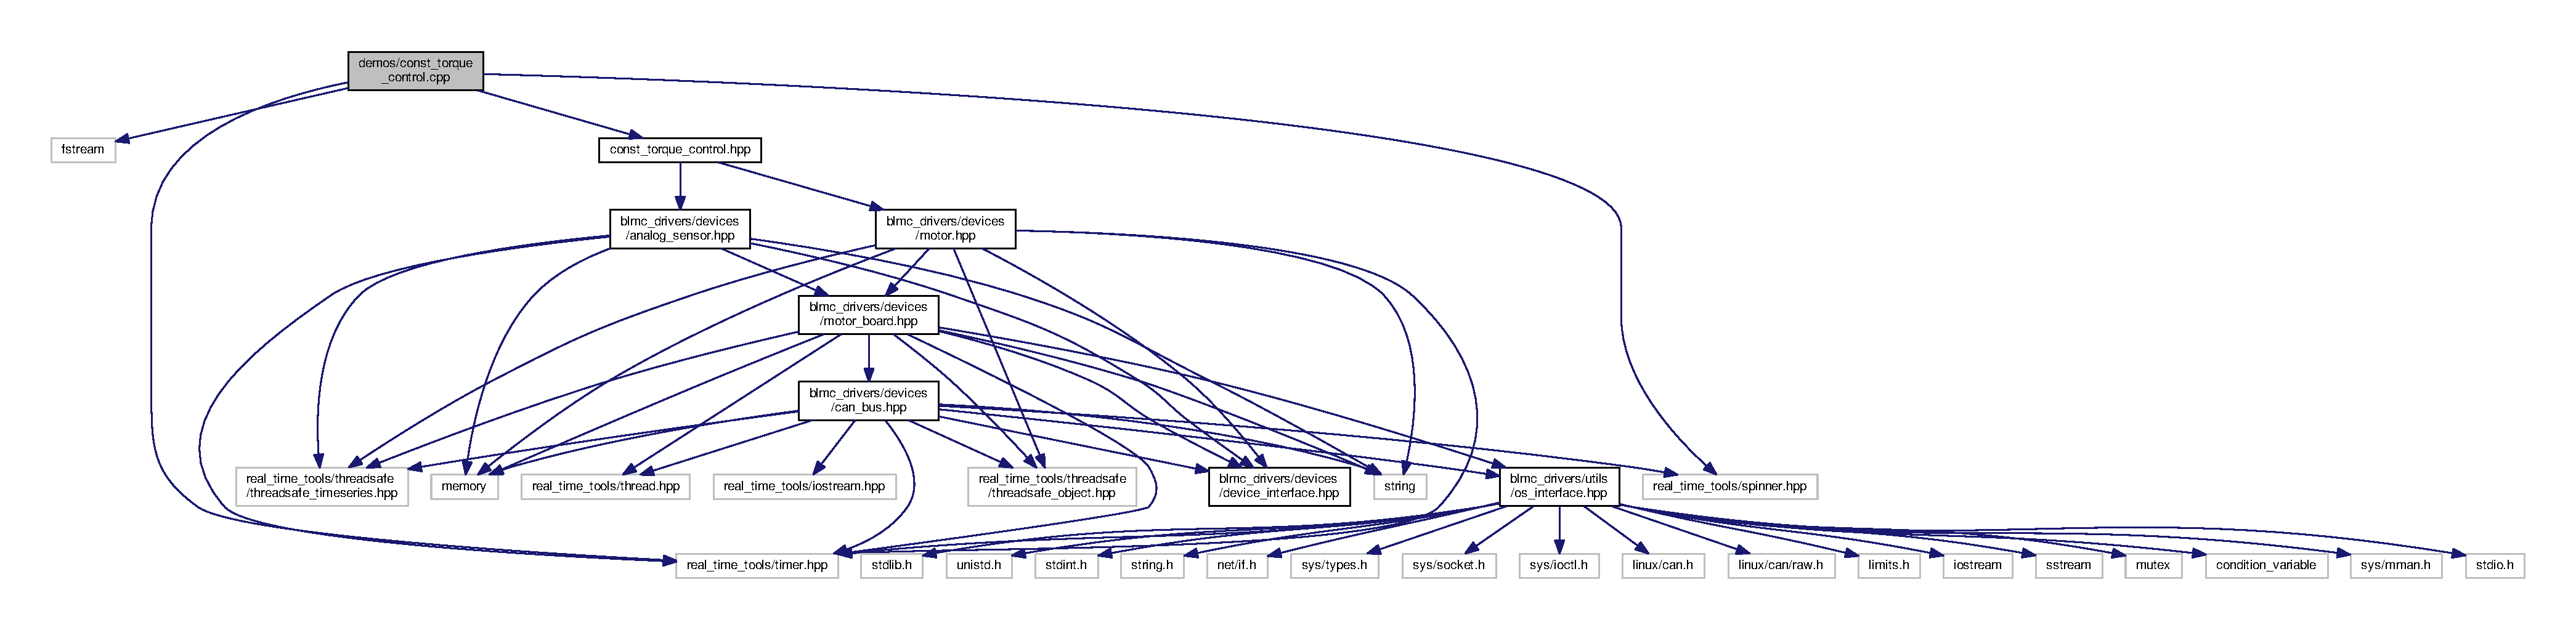
\includegraphics[width=350pt]{const__torque__control_8cpp__incl}
\end{center}
\end{figure}
\subsection*{Namespaces}
\begin{DoxyCompactItemize}
\item 
 \hyperlink{namespaceblmc__drivers}{blmc\+\_\+drivers}
\begin{DoxyCompactList}\small\item\em This namespace is the standard namespace of the package. \end{DoxyCompactList}\end{DoxyCompactItemize}


\subsection{Detailed Description}
\begin{DoxyCopyright}{Copyright}
Copyright (c) 2018-\/2020, New York University and Max Planck Gesellschaft, License B\+S\+D-\/3-\/\+Clause 
\end{DoxyCopyright}

\hypertarget{const__torque__control_8hpp}{}\section{demos/const\+\_\+torque\+\_\+control.hpp File Reference}
\label{const__torque__control_8hpp}\index{demos/const\+\_\+torque\+\_\+control.\+hpp@{demos/const\+\_\+torque\+\_\+control.\+hpp}}
{\ttfamily \#include \char`\"{}blmc\+\_\+drivers/devices/motor.\+hpp\char`\"{}}\\*
{\ttfamily \#include \char`\"{}blmc\+\_\+drivers/devices/analog\+\_\+sensor.\+hpp\char`\"{}}\\*
Include dependency graph for const\+\_\+torque\+\_\+control.\+hpp\+:
\nopagebreak
\begin{figure}[H]
\begin{center}
\leavevmode
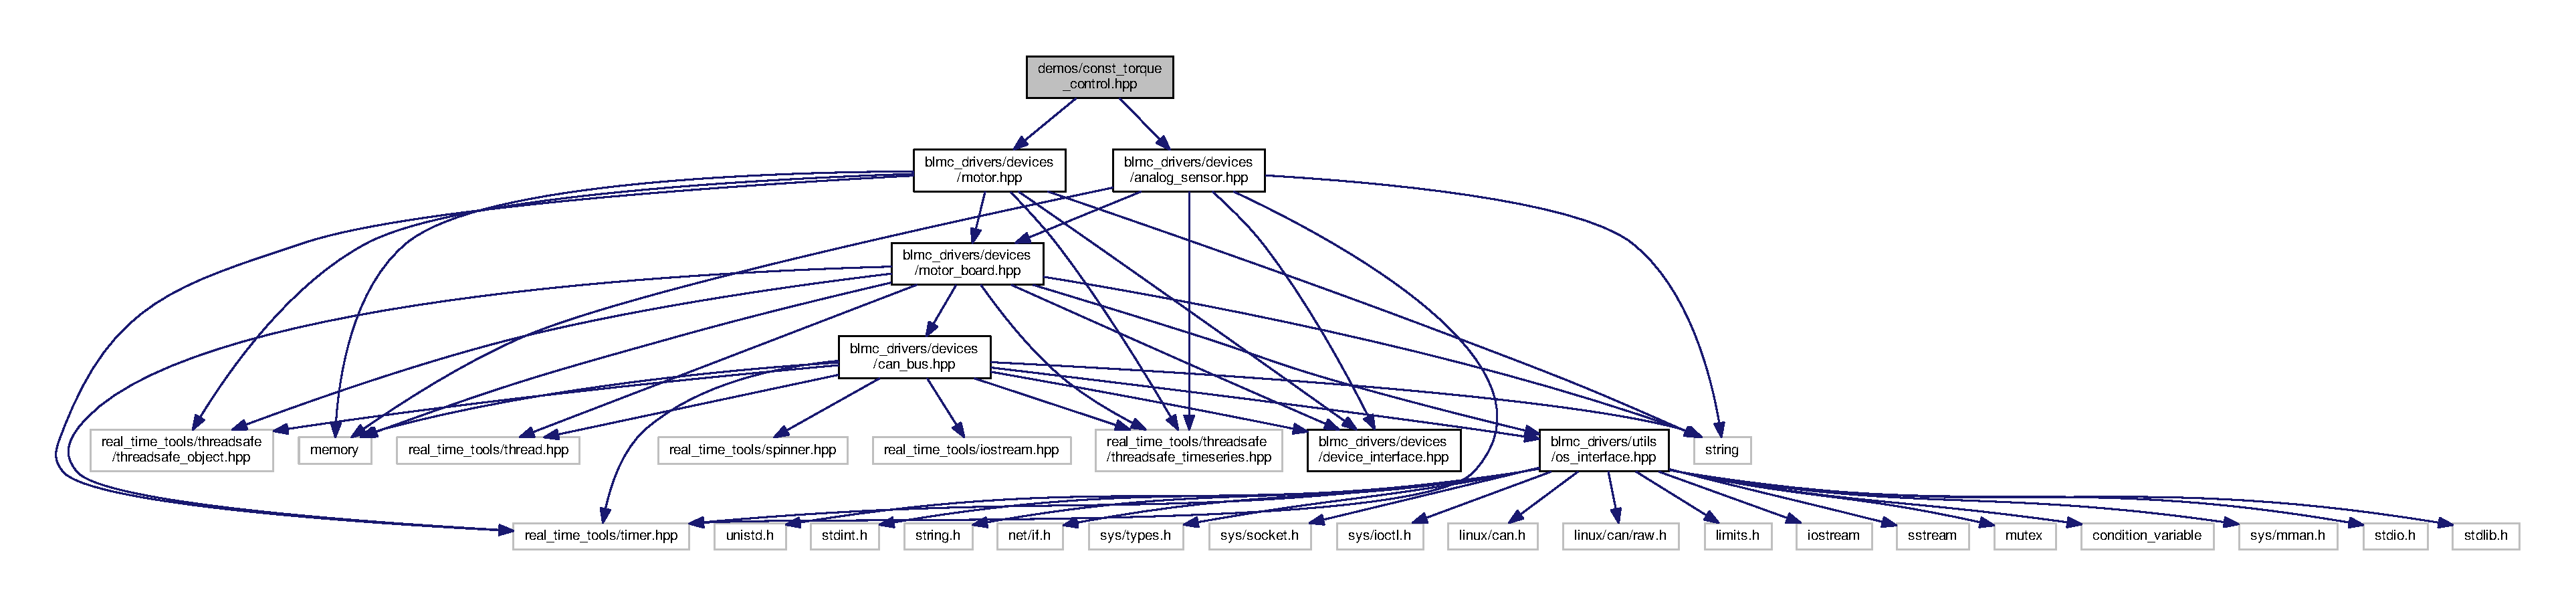
\includegraphics[width=350pt]{const__torque__control_8hpp__incl}
\end{center}
\end{figure}
This graph shows which files directly or indirectly include this file\+:
\nopagebreak
\begin{figure}[H]
\begin{center}
\leavevmode
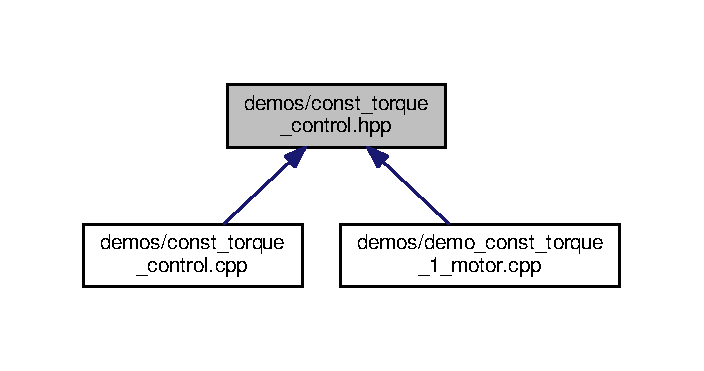
\includegraphics[width=338pt]{const__torque__control_8hpp__dep__incl}
\end{center}
\end{figure}
\subsection*{Classes}
\begin{DoxyCompactItemize}
\item 
class \hyperlink{classblmc__drivers_1_1ConstTorqueControl}{blmc\+\_\+drivers\+::\+Const\+Torque\+Control}
\begin{DoxyCompactList}\small\item\em This is a basic PD controller to be used in the demos of this package. \end{DoxyCompactList}\end{DoxyCompactItemize}
\subsection*{Namespaces}
\begin{DoxyCompactItemize}
\item 
 \hyperlink{namespaceblmc__drivers}{blmc\+\_\+drivers}
\begin{DoxyCompactList}\small\item\em This namespace is the standard namespace of the package. \end{DoxyCompactList}\end{DoxyCompactItemize}
\subsection*{Typedefs}
\begin{DoxyCompactItemize}
\item 
typedef std\+::shared\+\_\+ptr$<$ \hyperlink{classblmc__drivers_1_1SafeMotor}{blmc\+\_\+drivers\+::\+Safe\+Motor} $>$ \hyperlink{namespaceblmc__drivers_ab975c3be3c53a93a10c491f07a132e2b}{blmc\+\_\+drivers\+::\+Safe\+Motor\+\_\+ptr}\hypertarget{namespaceblmc__drivers_ab975c3be3c53a93a10c491f07a132e2b}{}\label{namespaceblmc__drivers_ab975c3be3c53a93a10c491f07a132e2b}

\begin{DoxyCompactList}\small\item\em This is a simple shortcut. \end{DoxyCompactList}\end{DoxyCompactItemize}


\subsection{Detailed Description}
\begin{DoxyCopyright}{Copyright}
Copyright (c) 2018-\/2020, New York University and Max Planck Gesellschaft, License B\+S\+D-\/3-\/\+Clause 
\end{DoxyCopyright}

\hypertarget{demo__1__motor_8cpp}{}\section{demos/demo\+\_\+1\+\_\+motor.cpp File Reference}
\label{demo__1__motor_8cpp}\index{demos/demo\+\_\+1\+\_\+motor.\+cpp@{demos/demo\+\_\+1\+\_\+motor.\+cpp}}
{\ttfamily \#include $<$tuple$>$}\\*
{\ttfamily \#include \char`\"{}blmc\+\_\+drivers/devices/can\+\_\+bus.\+hpp\char`\"{}}\\*
{\ttfamily \#include \char`\"{}blmc\+\_\+drivers/devices/motor\+\_\+board.\+hpp\char`\"{}}\\*
{\ttfamily \#include \char`\"{}blmc\+\_\+drivers/devices/motor.\+hpp\char`\"{}}\\*
{\ttfamily \#include \char`\"{}blmc\+\_\+drivers/devices/analog\+\_\+sensor.\+hpp\char`\"{}}\\*
Include dependency graph for demo\+\_\+1\+\_\+motor.\+cpp\+:
\nopagebreak
\begin{figure}[H]
\begin{center}
\leavevmode
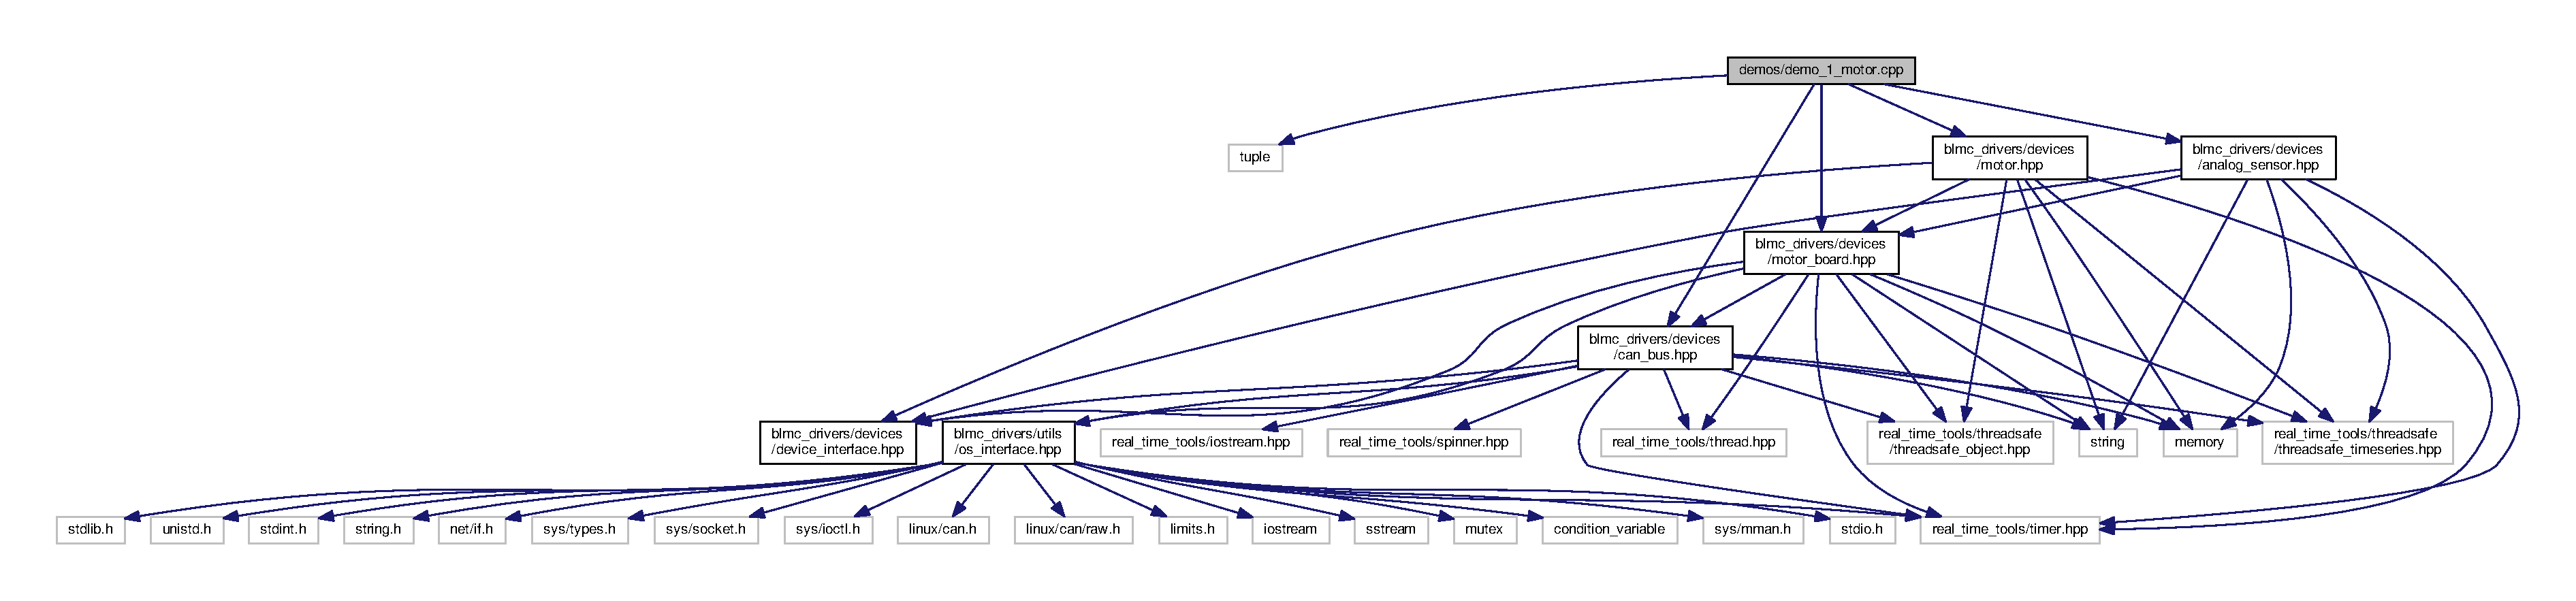
\includegraphics[width=350pt]{demo__1__motor_8cpp__incl}
\end{center}
\end{figure}
\subsection*{Classes}
\begin{DoxyCompactItemize}
\item 
struct \hyperlink{structHardware}{Hardware}
\end{DoxyCompactItemize}
\subsection*{Typedefs}
\begin{DoxyCompactItemize}
\item 
typedef std\+::tuple$<$ std\+::shared\+\_\+ptr$<$ \hyperlink{classblmc__drivers_1_1MotorInterface}{blmc\+\_\+drivers\+::\+Motor\+Interface} $>$, std\+::shared\+\_\+ptr$<$ \hyperlink{classblmc__drivers_1_1AnalogSensorInterface}{blmc\+\_\+drivers\+::\+Analog\+Sensor\+Interface} $>$ $>$ {\bfseries Motor\+And\+Slider}\hypertarget{demo__1__motor_8cpp_a9cef6c6e3b3a631ae41d5291a8107c2b}{}\label{demo__1__motor_8cpp_a9cef6c6e3b3a631ae41d5291a8107c2b}

\end{DoxyCompactItemize}
\subsection*{Functions}
\begin{DoxyCompactItemize}
\item 
static T\+H\+R\+E\+A\+D\+\_\+\+F\+U\+N\+C\+T\+I\+O\+N\+\_\+\+R\+E\+T\+U\+R\+N\+\_\+\+T\+Y\+PE {\bfseries control\+\_\+loop} (void $\ast$hardware\+\_\+ptr)\hypertarget{demo__1__motor_8cpp_a07b2980e601e477f63efb8dd69746cf6}{}\label{demo__1__motor_8cpp_a07b2980e601e477f63efb8dd69746cf6}

\item 
static T\+H\+R\+E\+A\+D\+\_\+\+F\+U\+N\+C\+T\+I\+O\+N\+\_\+\+R\+E\+T\+U\+R\+N\+\_\+\+T\+Y\+PE {\bfseries printing\+\_\+loop} (void $\ast$hardware\+\_\+ptr)\hypertarget{demo__1__motor_8cpp_ad18685f4cbdcd5b0f6f98059487b1203}{}\label{demo__1__motor_8cpp_ad18685f4cbdcd5b0f6f98059487b1203}

\item 
int {\bfseries main} (int argc, char $\ast$$\ast$argv)\hypertarget{demo__1__motor_8cpp_a3c04138a5bfe5d72780bb7e82a18e627}{}\label{demo__1__motor_8cpp_a3c04138a5bfe5d72780bb7e82a18e627}

\end{DoxyCompactItemize}


\subsection{Detailed Description}
\begin{DoxyCopyright}{Copyright}
Copyright (c) 2018-\/2020, New York University and Max Planck Gesellschaft, License B\+S\+D-\/3-\/\+Clause 
\end{DoxyCopyright}

\hypertarget{demo__1__motor__print__everything_8cpp}{}\section{demos/demo\+\_\+1\+\_\+motor\+\_\+print\+\_\+everything.cpp File Reference}
\label{demo__1__motor__print__everything_8cpp}\index{demos/demo\+\_\+1\+\_\+motor\+\_\+print\+\_\+everything.\+cpp@{demos/demo\+\_\+1\+\_\+motor\+\_\+print\+\_\+everything.\+cpp}}
{\ttfamily \#include $<$tuple$>$}\\*
{\ttfamily \#include \char`\"{}blmc\+\_\+drivers/devices/can\+\_\+bus.\+hpp\char`\"{}}\\*
{\ttfamily \#include \char`\"{}blmc\+\_\+drivers/devices/motor\+\_\+board.\+hpp\char`\"{}}\\*
{\ttfamily \#include \char`\"{}blmc\+\_\+drivers/devices/motor.\+hpp\char`\"{}}\\*
{\ttfamily \#include \char`\"{}blmc\+\_\+drivers/devices/analog\+\_\+sensor.\+hpp\char`\"{}}\\*
Include dependency graph for demo\+\_\+1\+\_\+motor\+\_\+print\+\_\+everything.\+cpp\+:
\nopagebreak
\begin{figure}[H]
\begin{center}
\leavevmode
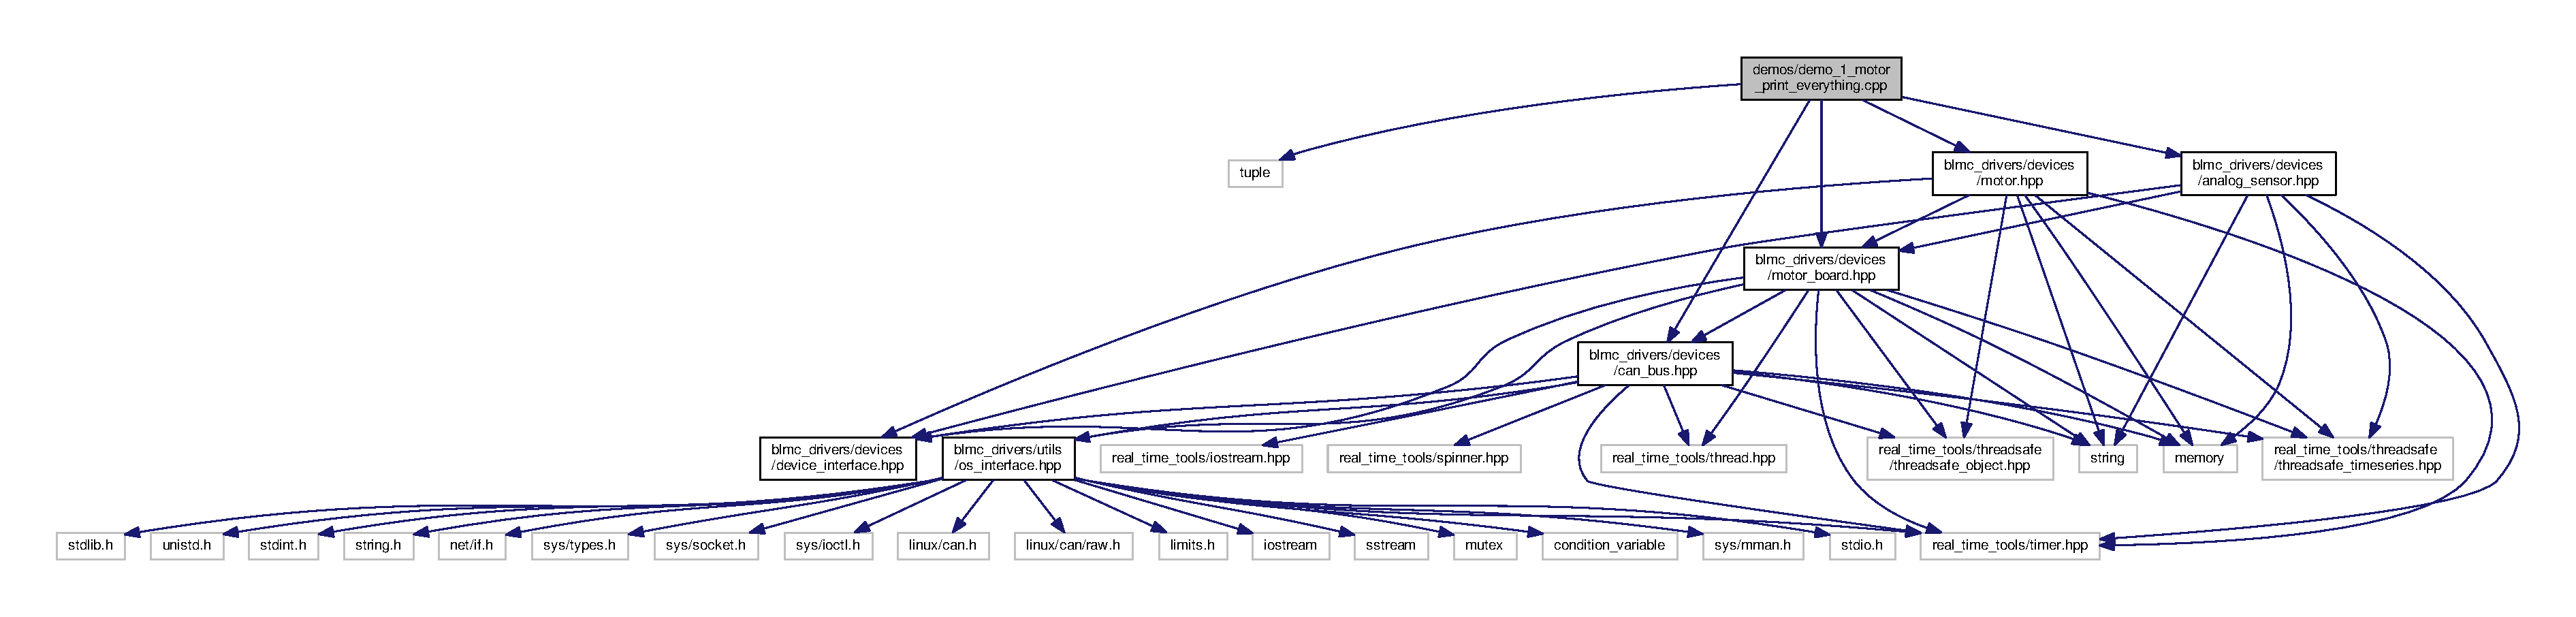
\includegraphics[width=350pt]{demo__1__motor__print__everything_8cpp__incl}
\end{center}
\end{figure}
\subsection*{Classes}
\begin{DoxyCompactItemize}
\item 
struct \hyperlink{structHardware}{Hardware}
\end{DoxyCompactItemize}
\subsection*{Typedefs}
\begin{DoxyCompactItemize}
\item 
typedef std\+::tuple$<$ std\+::shared\+\_\+ptr$<$ \hyperlink{classblmc__drivers_1_1MotorInterface}{blmc\+\_\+drivers\+::\+Motor\+Interface} $>$, std\+::shared\+\_\+ptr$<$ \hyperlink{classblmc__drivers_1_1AnalogSensorInterface}{blmc\+\_\+drivers\+::\+Analog\+Sensor\+Interface} $>$ $>$ {\bfseries Motor\+And\+Slider}\hypertarget{demo__1__motor__print__everything_8cpp_a79c0c6b6c32644638c116c33ac488cd1}{}\label{demo__1__motor__print__everything_8cpp_a79c0c6b6c32644638c116c33ac488cd1}

\end{DoxyCompactItemize}
\subsection*{Functions}
\begin{DoxyCompactItemize}
\item 
static T\+H\+R\+E\+A\+D\+\_\+\+F\+U\+N\+C\+T\+I\+O\+N\+\_\+\+R\+E\+T\+U\+R\+N\+\_\+\+T\+Y\+PE {\bfseries control\+\_\+loop} (void $\ast$hardware\+\_\+ptr)\hypertarget{demo__1__motor__print__everything_8cpp_a07b2980e601e477f63efb8dd69746cf6}{}\label{demo__1__motor__print__everything_8cpp_a07b2980e601e477f63efb8dd69746cf6}

\item 
static T\+H\+R\+E\+A\+D\+\_\+\+F\+U\+N\+C\+T\+I\+O\+N\+\_\+\+R\+E\+T\+U\+R\+N\+\_\+\+T\+Y\+PE {\bfseries printing\+\_\+loop} (void $\ast$hardware\+\_\+ptr)\hypertarget{demo__1__motor__print__everything_8cpp_ad18685f4cbdcd5b0f6f98059487b1203}{}\label{demo__1__motor__print__everything_8cpp_ad18685f4cbdcd5b0f6f98059487b1203}

\item 
int {\bfseries main} (int, char $\ast$$\ast$)\hypertarget{demo__1__motor__print__everything_8cpp_a2c3f6775325c30275d11c6abee2db6a0}{}\label{demo__1__motor__print__everything_8cpp_a2c3f6775325c30275d11c6abee2db6a0}

\end{DoxyCompactItemize}


\subsection{Detailed Description}
\begin{DoxyCopyright}{Copyright}
Copyright (c) 2018-\/2020, New York University and Max Planck Gesellschaft, License B\+S\+D-\/3-\/\+Clause 
\end{DoxyCopyright}

\hypertarget{demo__2__motors_8cpp}{}\section{demos/demo\+\_\+2\+\_\+motors.cpp File Reference}
\label{demo__2__motors_8cpp}\index{demos/demo\+\_\+2\+\_\+motors.\+cpp@{demos/demo\+\_\+2\+\_\+motors.\+cpp}}
{\ttfamily \#include $<$atomic$>$}\\*
{\ttfamily \#include $<$signal.\+h$>$}\\*
{\ttfamily \#include $<$pd\+\_\+control.\+hpp$>$}\\*
Include dependency graph for demo\+\_\+2\+\_\+motors.\+cpp\+:
\nopagebreak
\begin{figure}[H]
\begin{center}
\leavevmode
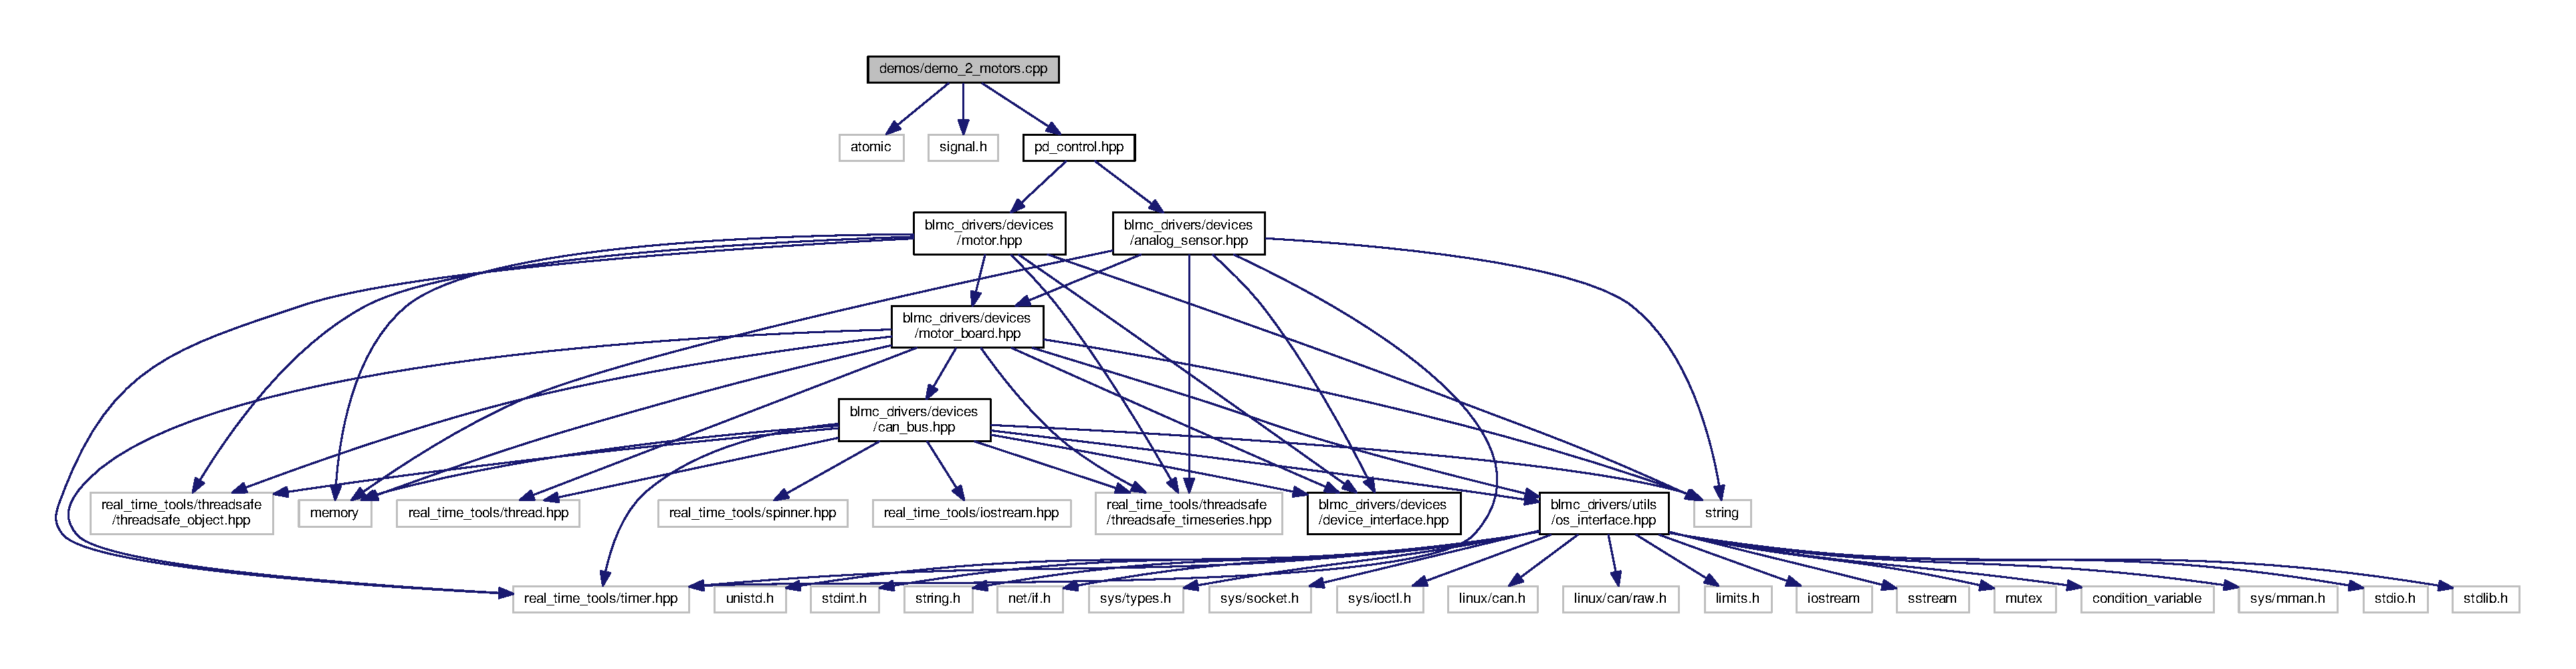
\includegraphics[width=350pt]{demo__2__motors_8cpp__incl}
\end{center}
\end{figure}
\subsection*{Functions}
\begin{DoxyCompactItemize}
\item 
std\+::atomic\+\_\+bool \hyperlink{demo__2__motors_8cpp_a75d8b98fafbd2fb243e91c6164b114ce}{Stop\+Demos} (false)\hypertarget{demo__2__motors_8cpp_a75d8b98fafbd2fb243e91c6164b114ce}{}\label{demo__2__motors_8cpp_a75d8b98fafbd2fb243e91c6164b114ce}

\begin{DoxyCompactList}\small\item\em This boolean is here to kill cleanly the application upon ctrl+c. \end{DoxyCompactList}\item 
void \hyperlink{demo__2__motors_8cpp_a3d51efaeecab2023836cefe28d4dcff4}{my\+\_\+handler} (int)
\begin{DoxyCompactList}\small\item\em This function is the callback upon a ctrl+c call from the terminal. \end{DoxyCompactList}\item 
int \hyperlink{demo__2__motors_8cpp_a2c3f6775325c30275d11c6abee2db6a0}{main} (int, char $\ast$$\ast$)
\begin{DoxyCompactList}\small\item\em This is the main demo program. \end{DoxyCompactList}\end{DoxyCompactItemize}


\subsection{Detailed Description}
\begin{DoxyCopyright}{Copyright}
Copyright (c) 2018-\/2020, New York University and Max Planck Gesellschaft, License B\+S\+D-\/3-\/\+Clause 
\end{DoxyCopyright}


\subsection{Function Documentation}
\index{demo\+\_\+2\+\_\+motors.\+cpp@{demo\+\_\+2\+\_\+motors.\+cpp}!main@{main}}
\index{main@{main}!demo\+\_\+2\+\_\+motors.\+cpp@{demo\+\_\+2\+\_\+motors.\+cpp}}
\subsubsection[{\texorpdfstring{main(int, char $\ast$$\ast$)}{main(int, char **)}}]{\setlength{\rightskip}{0pt plus 5cm}int main (
\begin{DoxyParamCaption}
\item[{int}]{, }
\item[{char $\ast$$\ast$}]{}
\end{DoxyParamCaption}
)}\hypertarget{demo__2__motors_8cpp_a2c3f6775325c30275d11c6abee2db6a0}{}\label{demo__2__motors_8cpp_a2c3f6775325c30275d11c6abee2db6a0}


This is the main demo program. 


\begin{DoxyParams}{Parameters}
{\em argc} & \\
\hline
{\em argv} & \\
\hline
\end{DoxyParams}
\begin{DoxyReturn}{Returns}
int 
\end{DoxyReturn}
\index{demo\+\_\+2\+\_\+motors.\+cpp@{demo\+\_\+2\+\_\+motors.\+cpp}!my\+\_\+handler@{my\+\_\+handler}}
\index{my\+\_\+handler@{my\+\_\+handler}!demo\+\_\+2\+\_\+motors.\+cpp@{demo\+\_\+2\+\_\+motors.\+cpp}}
\subsubsection[{\texorpdfstring{my\+\_\+handler(int)}{my_handler(int)}}]{\setlength{\rightskip}{0pt plus 5cm}void my\+\_\+handler (
\begin{DoxyParamCaption}
\item[{int}]{}
\end{DoxyParamCaption}
)}\hypertarget{demo__2__motors_8cpp_a3d51efaeecab2023836cefe28d4dcff4}{}\label{demo__2__motors_8cpp_a3d51efaeecab2023836cefe28d4dcff4}


This function is the callback upon a ctrl+c call from the terminal. 


\begin{DoxyParams}{Parameters}
{\em s} & \\
\hline
\end{DoxyParams}

\hypertarget{demo__3__motors_8cpp}{}\section{demos/demo\+\_\+3\+\_\+motors.cpp File Reference}
\label{demo__3__motors_8cpp}\index{demos/demo\+\_\+3\+\_\+motors.\+cpp@{demos/demo\+\_\+3\+\_\+motors.\+cpp}}
{\ttfamily \#include $<$atomic$>$}\\*
{\ttfamily \#include $<$signal.\+h$>$}\\*
{\ttfamily \#include \char`\"{}pd\+\_\+control.\+hpp\char`\"{}}\\*
Include dependency graph for demo\+\_\+3\+\_\+motors.\+cpp\+:
\nopagebreak
\begin{figure}[H]
\begin{center}
\leavevmode
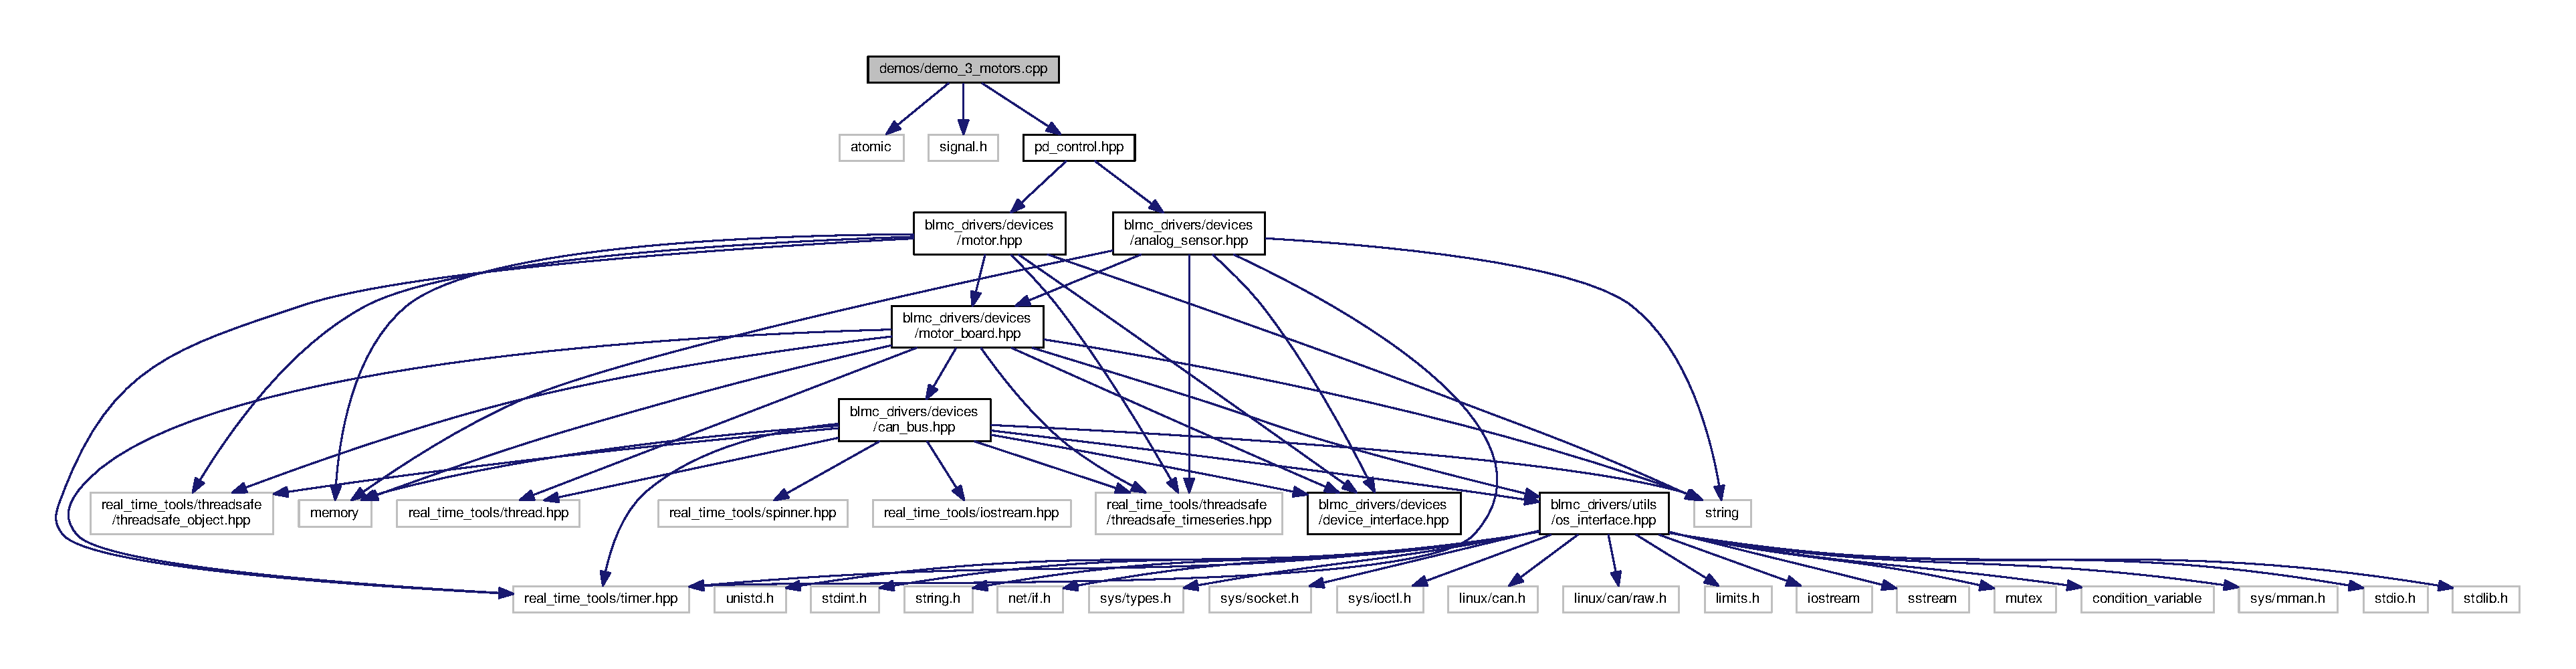
\includegraphics[width=350pt]{demo__3__motors_8cpp__incl}
\end{center}
\end{figure}
\subsection*{Functions}
\begin{DoxyCompactItemize}
\item 
std\+::atomic\+\_\+bool \hyperlink{demo__3__motors_8cpp_a75d8b98fafbd2fb243e91c6164b114ce}{Stop\+Demos} (false)\hypertarget{demo__3__motors_8cpp_a75d8b98fafbd2fb243e91c6164b114ce}{}\label{demo__3__motors_8cpp_a75d8b98fafbd2fb243e91c6164b114ce}

\begin{DoxyCompactList}\small\item\em This boolean is here to kill cleanly the application upon ctrl+c. \end{DoxyCompactList}\item 
void \hyperlink{demo__3__motors_8cpp_a13848d945610347db87a059fe0b43f35}{my\+\_\+handler} (int s)
\begin{DoxyCompactList}\small\item\em This function is the callback upon a ctrl+c call from the terminal. \end{DoxyCompactList}\item 
int \hyperlink{demo__3__motors_8cpp_a3c04138a5bfe5d72780bb7e82a18e627}{main} (int argc, char $\ast$$\ast$argv)
\begin{DoxyCompactList}\small\item\em This is the main demo program. \end{DoxyCompactList}\end{DoxyCompactItemize}


\subsection{Detailed Description}
\begin{DoxyCopyright}{Copyright}
Copyright (c) 2018-\/2020, New York University and Max Planck Gesellschaft, License B\+S\+D-\/3-\/\+Clause 
\end{DoxyCopyright}


\subsection{Function Documentation}
\index{demo\+\_\+3\+\_\+motors.\+cpp@{demo\+\_\+3\+\_\+motors.\+cpp}!main@{main}}
\index{main@{main}!demo\+\_\+3\+\_\+motors.\+cpp@{demo\+\_\+3\+\_\+motors.\+cpp}}
\subsubsection[{\texorpdfstring{main(int argc, char $\ast$$\ast$argv)}{main(int argc, char **argv)}}]{\setlength{\rightskip}{0pt plus 5cm}int main (
\begin{DoxyParamCaption}
\item[{int}]{argc, }
\item[{char $\ast$$\ast$}]{argv}
\end{DoxyParamCaption}
)}\hypertarget{demo__3__motors_8cpp_a3c04138a5bfe5d72780bb7e82a18e627}{}\label{demo__3__motors_8cpp_a3c04138a5bfe5d72780bb7e82a18e627}


This is the main demo program. 


\begin{DoxyParams}{Parameters}
{\em argc} & \\
\hline
{\em argv} & \\
\hline
\end{DoxyParams}
\begin{DoxyReturn}{Returns}
int 
\end{DoxyReturn}
\index{demo\+\_\+3\+\_\+motors.\+cpp@{demo\+\_\+3\+\_\+motors.\+cpp}!my\+\_\+handler@{my\+\_\+handler}}
\index{my\+\_\+handler@{my\+\_\+handler}!demo\+\_\+3\+\_\+motors.\+cpp@{demo\+\_\+3\+\_\+motors.\+cpp}}
\subsubsection[{\texorpdfstring{my\+\_\+handler(int s)}{my_handler(int s)}}]{\setlength{\rightskip}{0pt plus 5cm}void my\+\_\+handler (
\begin{DoxyParamCaption}
\item[{int}]{s}
\end{DoxyParamCaption}
)}\hypertarget{demo__3__motors_8cpp_a13848d945610347db87a059fe0b43f35}{}\label{demo__3__motors_8cpp_a13848d945610347db87a059fe0b43f35}


This function is the callback upon a ctrl+c call from the terminal. 


\begin{DoxyParams}{Parameters}
{\em s} & \\
\hline
\end{DoxyParams}

\hypertarget{demo__8__motors_8cpp}{}\section{demos/demo\+\_\+8\+\_\+motors.cpp File Reference}
\label{demo__8__motors_8cpp}\index{demos/demo\+\_\+8\+\_\+motors.\+cpp@{demos/demo\+\_\+8\+\_\+motors.\+cpp}}
{\ttfamily \#include $<$atomic$>$}\\*
{\ttfamily \#include $<$signal.\+h$>$}\\*
{\ttfamily \#include $<$pd\+\_\+control.\+hpp$>$}\\*
Include dependency graph for demo\+\_\+8\+\_\+motors.\+cpp\+:
\nopagebreak
\begin{figure}[H]
\begin{center}
\leavevmode
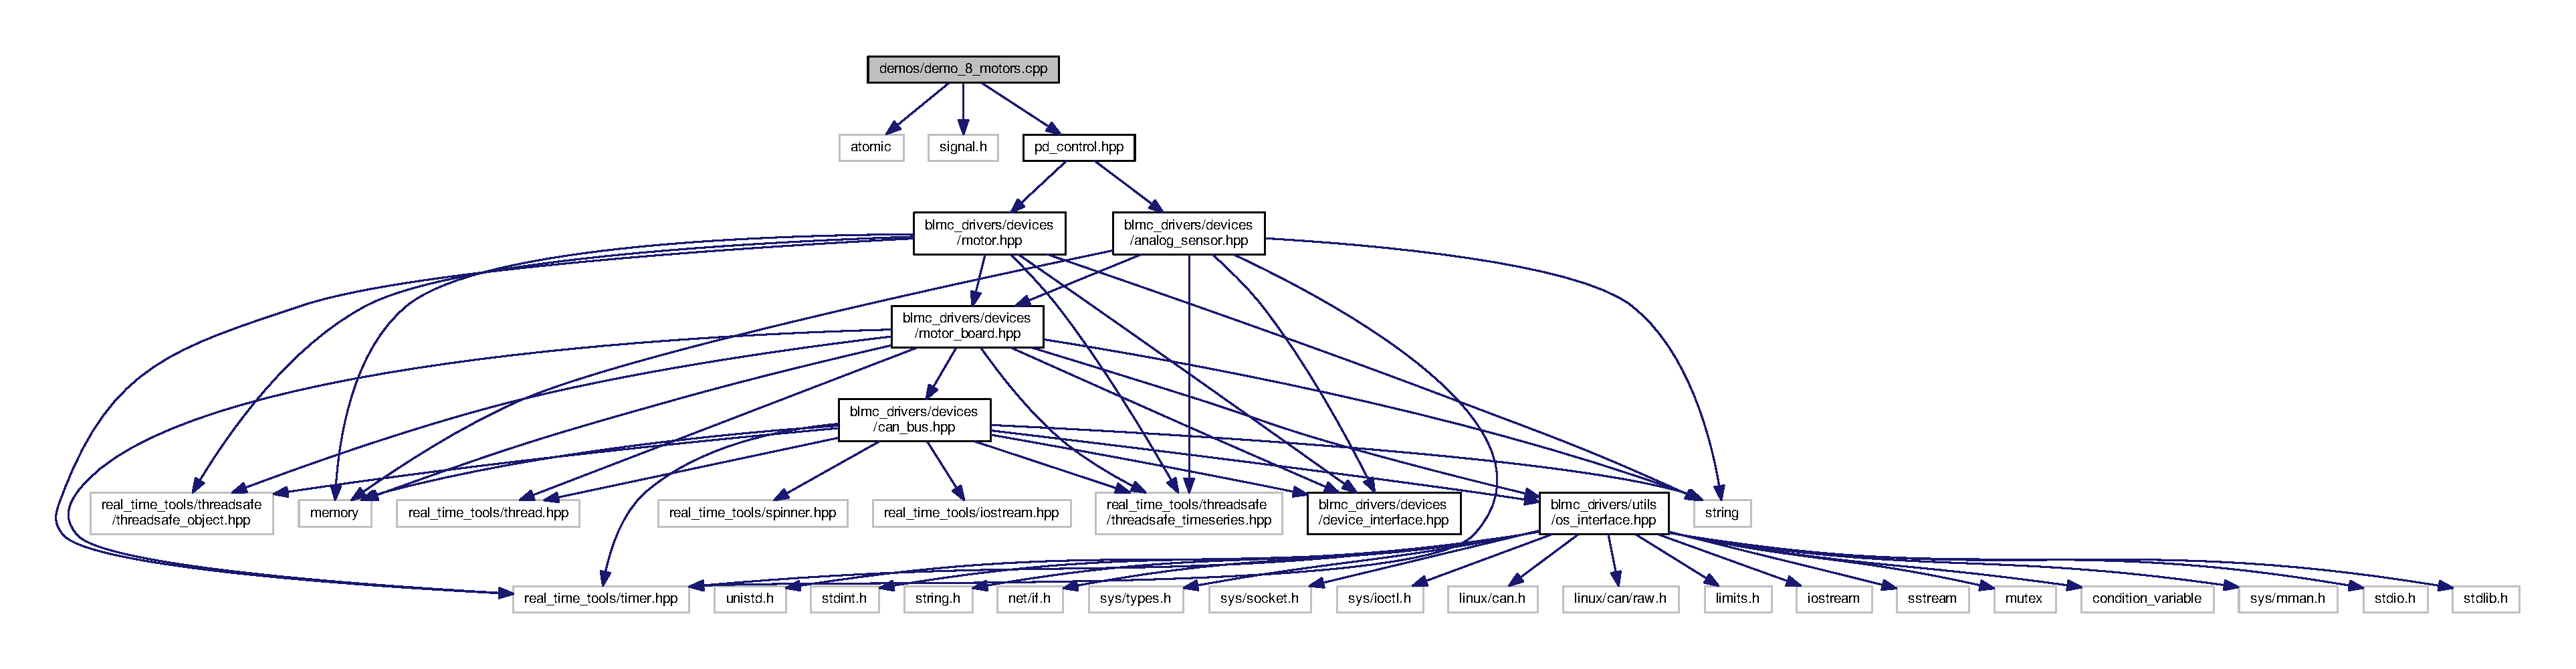
\includegraphics[width=350pt]{demo__8__motors_8cpp__incl}
\end{center}
\end{figure}
\subsection*{Functions}
\begin{DoxyCompactItemize}
\item 
std\+::atomic\+\_\+bool \hyperlink{demo__8__motors_8cpp_a75d8b98fafbd2fb243e91c6164b114ce}{Stop\+Demos} (false)\hypertarget{demo__8__motors_8cpp_a75d8b98fafbd2fb243e91c6164b114ce}{}\label{demo__8__motors_8cpp_a75d8b98fafbd2fb243e91c6164b114ce}

\begin{DoxyCompactList}\small\item\em This boolean is here to kill cleanly the application upon ctrl+c. \end{DoxyCompactList}\item 
void \hyperlink{demo__8__motors_8cpp_a3d51efaeecab2023836cefe28d4dcff4}{my\+\_\+handler} (int)
\begin{DoxyCompactList}\small\item\em This function is the callback upon a ctrl+c call from the terminal. \end{DoxyCompactList}\item 
int \hyperlink{demo__8__motors_8cpp_a2c3f6775325c30275d11c6abee2db6a0}{main} (int, char $\ast$$\ast$)
\begin{DoxyCompactList}\small\item\em This is the main demo program. \end{DoxyCompactList}\end{DoxyCompactItemize}


\subsection{Detailed Description}
\begin{DoxyCopyright}{Copyright}
Copyright (c) 2018-\/2020, New York University and Max Planck Gesellschaft, License B\+S\+D-\/3-\/\+Clause 
\end{DoxyCopyright}


\subsection{Function Documentation}
\index{demo\+\_\+8\+\_\+motors.\+cpp@{demo\+\_\+8\+\_\+motors.\+cpp}!main@{main}}
\index{main@{main}!demo\+\_\+8\+\_\+motors.\+cpp@{demo\+\_\+8\+\_\+motors.\+cpp}}
\subsubsection[{\texorpdfstring{main(int, char $\ast$$\ast$)}{main(int, char **)}}]{\setlength{\rightskip}{0pt plus 5cm}int main (
\begin{DoxyParamCaption}
\item[{int}]{, }
\item[{char $\ast$$\ast$}]{}
\end{DoxyParamCaption}
)}\hypertarget{demo__8__motors_8cpp_a2c3f6775325c30275d11c6abee2db6a0}{}\label{demo__8__motors_8cpp_a2c3f6775325c30275d11c6abee2db6a0}


This is the main demo program. 


\begin{DoxyParams}{Parameters}
{\em argc} & \\
\hline
{\em argv} & \\
\hline
\end{DoxyParams}
\begin{DoxyReturn}{Returns}
int 
\end{DoxyReturn}
\index{demo\+\_\+8\+\_\+motors.\+cpp@{demo\+\_\+8\+\_\+motors.\+cpp}!my\+\_\+handler@{my\+\_\+handler}}
\index{my\+\_\+handler@{my\+\_\+handler}!demo\+\_\+8\+\_\+motors.\+cpp@{demo\+\_\+8\+\_\+motors.\+cpp}}
\subsubsection[{\texorpdfstring{my\+\_\+handler(int)}{my_handler(int)}}]{\setlength{\rightskip}{0pt plus 5cm}void my\+\_\+handler (
\begin{DoxyParamCaption}
\item[{int}]{}
\end{DoxyParamCaption}
)}\hypertarget{demo__8__motors_8cpp_a3d51efaeecab2023836cefe28d4dcff4}{}\label{demo__8__motors_8cpp_a3d51efaeecab2023836cefe28d4dcff4}


This function is the callback upon a ctrl+c call from the terminal. 


\begin{DoxyParams}{Parameters}
{\em s} & \\
\hline
\end{DoxyParams}

\hypertarget{demo__const__torque__1__motor_8cpp}{}\section{demos/demo\+\_\+const\+\_\+torque\+\_\+1\+\_\+motor.cpp File Reference}
\label{demo__const__torque__1__motor_8cpp}\index{demos/demo\+\_\+const\+\_\+torque\+\_\+1\+\_\+motor.\+cpp@{demos/demo\+\_\+const\+\_\+torque\+\_\+1\+\_\+motor.\+cpp}}
{\ttfamily \#include $<$atomic$>$}\\*
{\ttfamily \#include $<$signal.\+h$>$}\\*
{\ttfamily \#include \char`\"{}const\+\_\+torque\+\_\+control.\+hpp\char`\"{}}\\*
Include dependency graph for demo\+\_\+const\+\_\+torque\+\_\+1\+\_\+motor.\+cpp\+:
\nopagebreak
\begin{figure}[H]
\begin{center}
\leavevmode
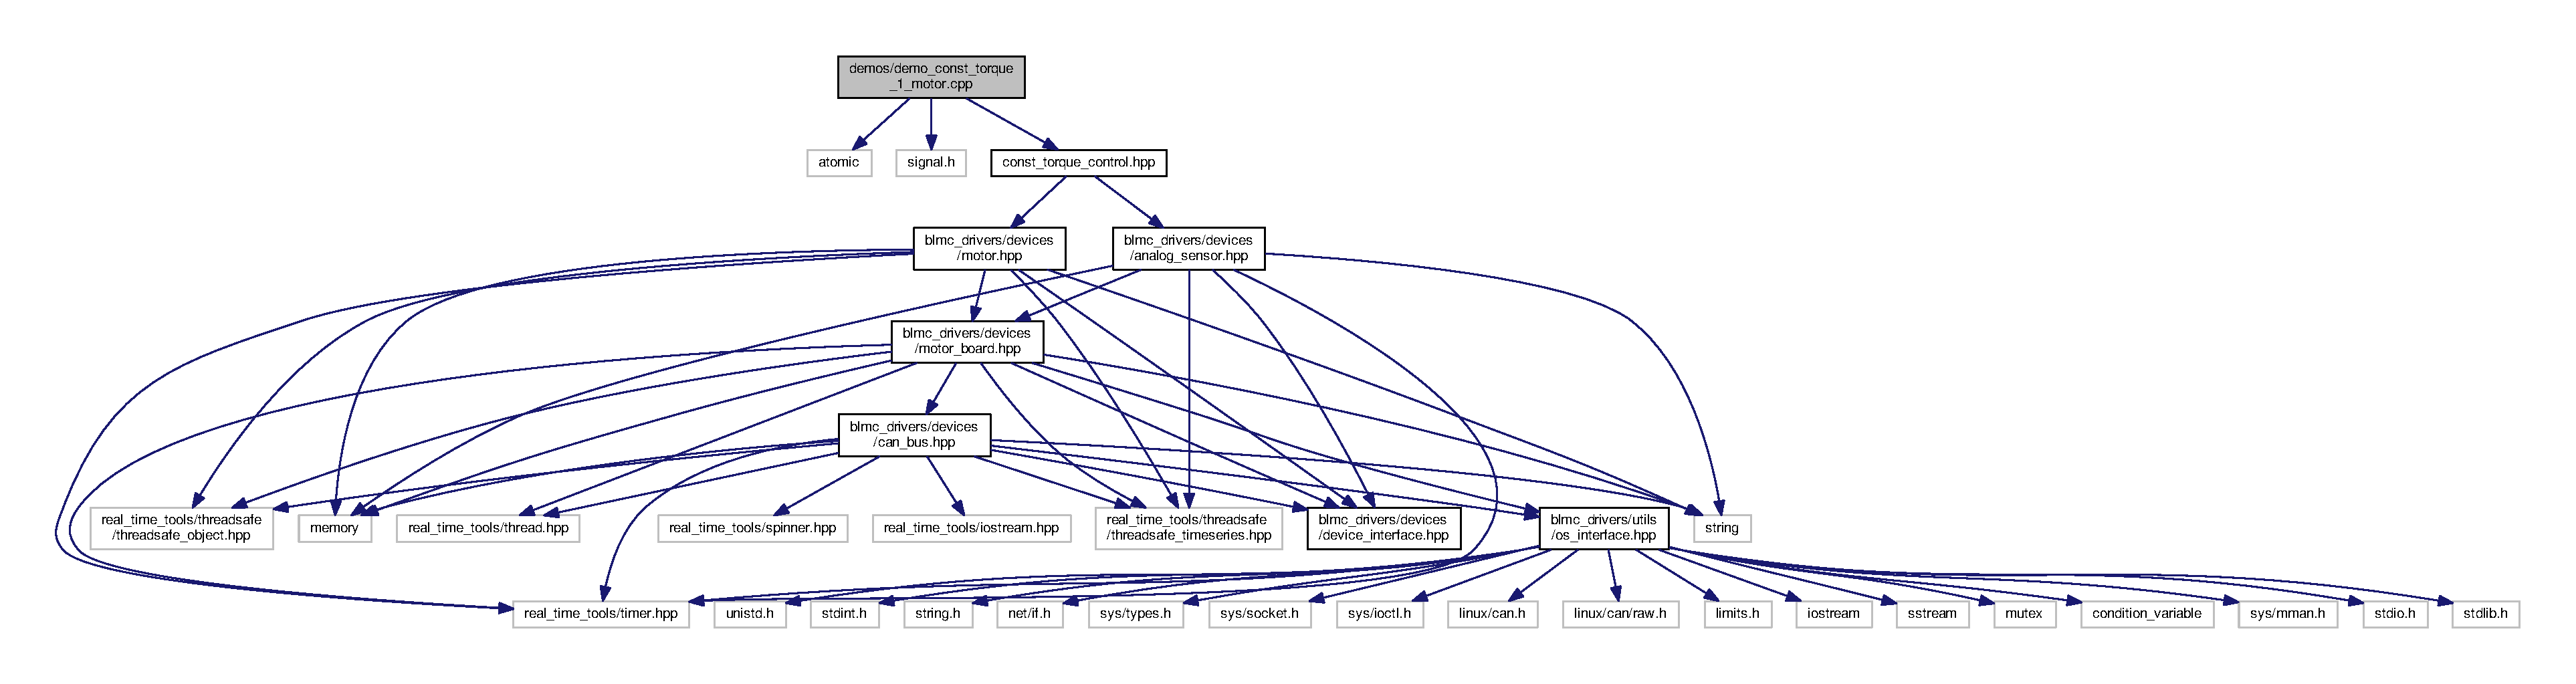
\includegraphics[width=350pt]{demo__const__torque__1__motor_8cpp__incl}
\end{center}
\end{figure}
\subsection*{Functions}
\begin{DoxyCompactItemize}
\item 
std\+::atomic\+\_\+bool \hyperlink{demo__const__torque__1__motor_8cpp_a75d8b98fafbd2fb243e91c6164b114ce}{Stop\+Demos} (false)\hypertarget{demo__const__torque__1__motor_8cpp_a75d8b98fafbd2fb243e91c6164b114ce}{}\label{demo__const__torque__1__motor_8cpp_a75d8b98fafbd2fb243e91c6164b114ce}

\begin{DoxyCompactList}\small\item\em This boolean is here to kill cleanly the application upon ctrl+c. \end{DoxyCompactList}\item 
void \hyperlink{demo__const__torque__1__motor_8cpp_a3d51efaeecab2023836cefe28d4dcff4}{my\+\_\+handler} (int)
\begin{DoxyCompactList}\small\item\em This function is the callback upon a ctrl+c call from the terminal. \end{DoxyCompactList}\item 
int \hyperlink{demo__const__torque__1__motor_8cpp_a2c3f6775325c30275d11c6abee2db6a0}{main} (int, char $\ast$$\ast$)
\begin{DoxyCompactList}\small\item\em This is the main demo program. \end{DoxyCompactList}\end{DoxyCompactItemize}


\subsection{Detailed Description}
\begin{DoxyCopyright}{Copyright}
Copyright (c) 2018-\/2020, New York University and Max Planck Gesellschaft, License B\+S\+D-\/3-\/\+Clause 
\end{DoxyCopyright}


\subsection{Function Documentation}
\index{demo\+\_\+const\+\_\+torque\+\_\+1\+\_\+motor.\+cpp@{demo\+\_\+const\+\_\+torque\+\_\+1\+\_\+motor.\+cpp}!main@{main}}
\index{main@{main}!demo\+\_\+const\+\_\+torque\+\_\+1\+\_\+motor.\+cpp@{demo\+\_\+const\+\_\+torque\+\_\+1\+\_\+motor.\+cpp}}
\subsubsection[{\texorpdfstring{main(int, char $\ast$$\ast$)}{main(int, char **)}}]{\setlength{\rightskip}{0pt plus 5cm}int main (
\begin{DoxyParamCaption}
\item[{int}]{, }
\item[{char $\ast$$\ast$}]{}
\end{DoxyParamCaption}
)}\hypertarget{demo__const__torque__1__motor_8cpp_a2c3f6775325c30275d11c6abee2db6a0}{}\label{demo__const__torque__1__motor_8cpp_a2c3f6775325c30275d11c6abee2db6a0}


This is the main demo program. 


\begin{DoxyParams}{Parameters}
{\em argc} & \\
\hline
{\em argv} & \\
\hline
\end{DoxyParams}
\begin{DoxyReturn}{Returns}
int 
\end{DoxyReturn}
\index{demo\+\_\+const\+\_\+torque\+\_\+1\+\_\+motor.\+cpp@{demo\+\_\+const\+\_\+torque\+\_\+1\+\_\+motor.\+cpp}!my\+\_\+handler@{my\+\_\+handler}}
\index{my\+\_\+handler@{my\+\_\+handler}!demo\+\_\+const\+\_\+torque\+\_\+1\+\_\+motor.\+cpp@{demo\+\_\+const\+\_\+torque\+\_\+1\+\_\+motor.\+cpp}}
\subsubsection[{\texorpdfstring{my\+\_\+handler(int)}{my_handler(int)}}]{\setlength{\rightskip}{0pt plus 5cm}void my\+\_\+handler (
\begin{DoxyParamCaption}
\item[{int}]{}
\end{DoxyParamCaption}
)}\hypertarget{demo__const__torque__1__motor_8cpp_a3d51efaeecab2023836cefe28d4dcff4}{}\label{demo__const__torque__1__motor_8cpp_a3d51efaeecab2023836cefe28d4dcff4}


This function is the callback upon a ctrl+c call from the terminal. 


\begin{DoxyParams}{Parameters}
{\em s} & \\
\hline
\end{DoxyParams}

\hypertarget{demo__ethernet_8cpp}{}\section{demos/demo\+\_\+ethernet.cpp File Reference}
\label{demo__ethernet_8cpp}\index{demos/demo\+\_\+ethernet.\+cpp@{demos/demo\+\_\+ethernet.\+cpp}}
{\ttfamily \#include $<$atomic$>$}\\*
{\ttfamily \#include $<$signal.\+h$>$}\\*
{\ttfamily \#include \char`\"{}blmc\+\_\+drivers/devices/spi\+\_\+motor\+\_\+board.\+hpp\char`\"{}}\\*
{\ttfamily \#include \char`\"{}sine\+\_\+position\+\_\+control.\+hpp\char`\"{}}\\*
Include dependency graph for demo\+\_\+ethernet.\+cpp\+:
\nopagebreak
\begin{figure}[H]
\begin{center}
\leavevmode
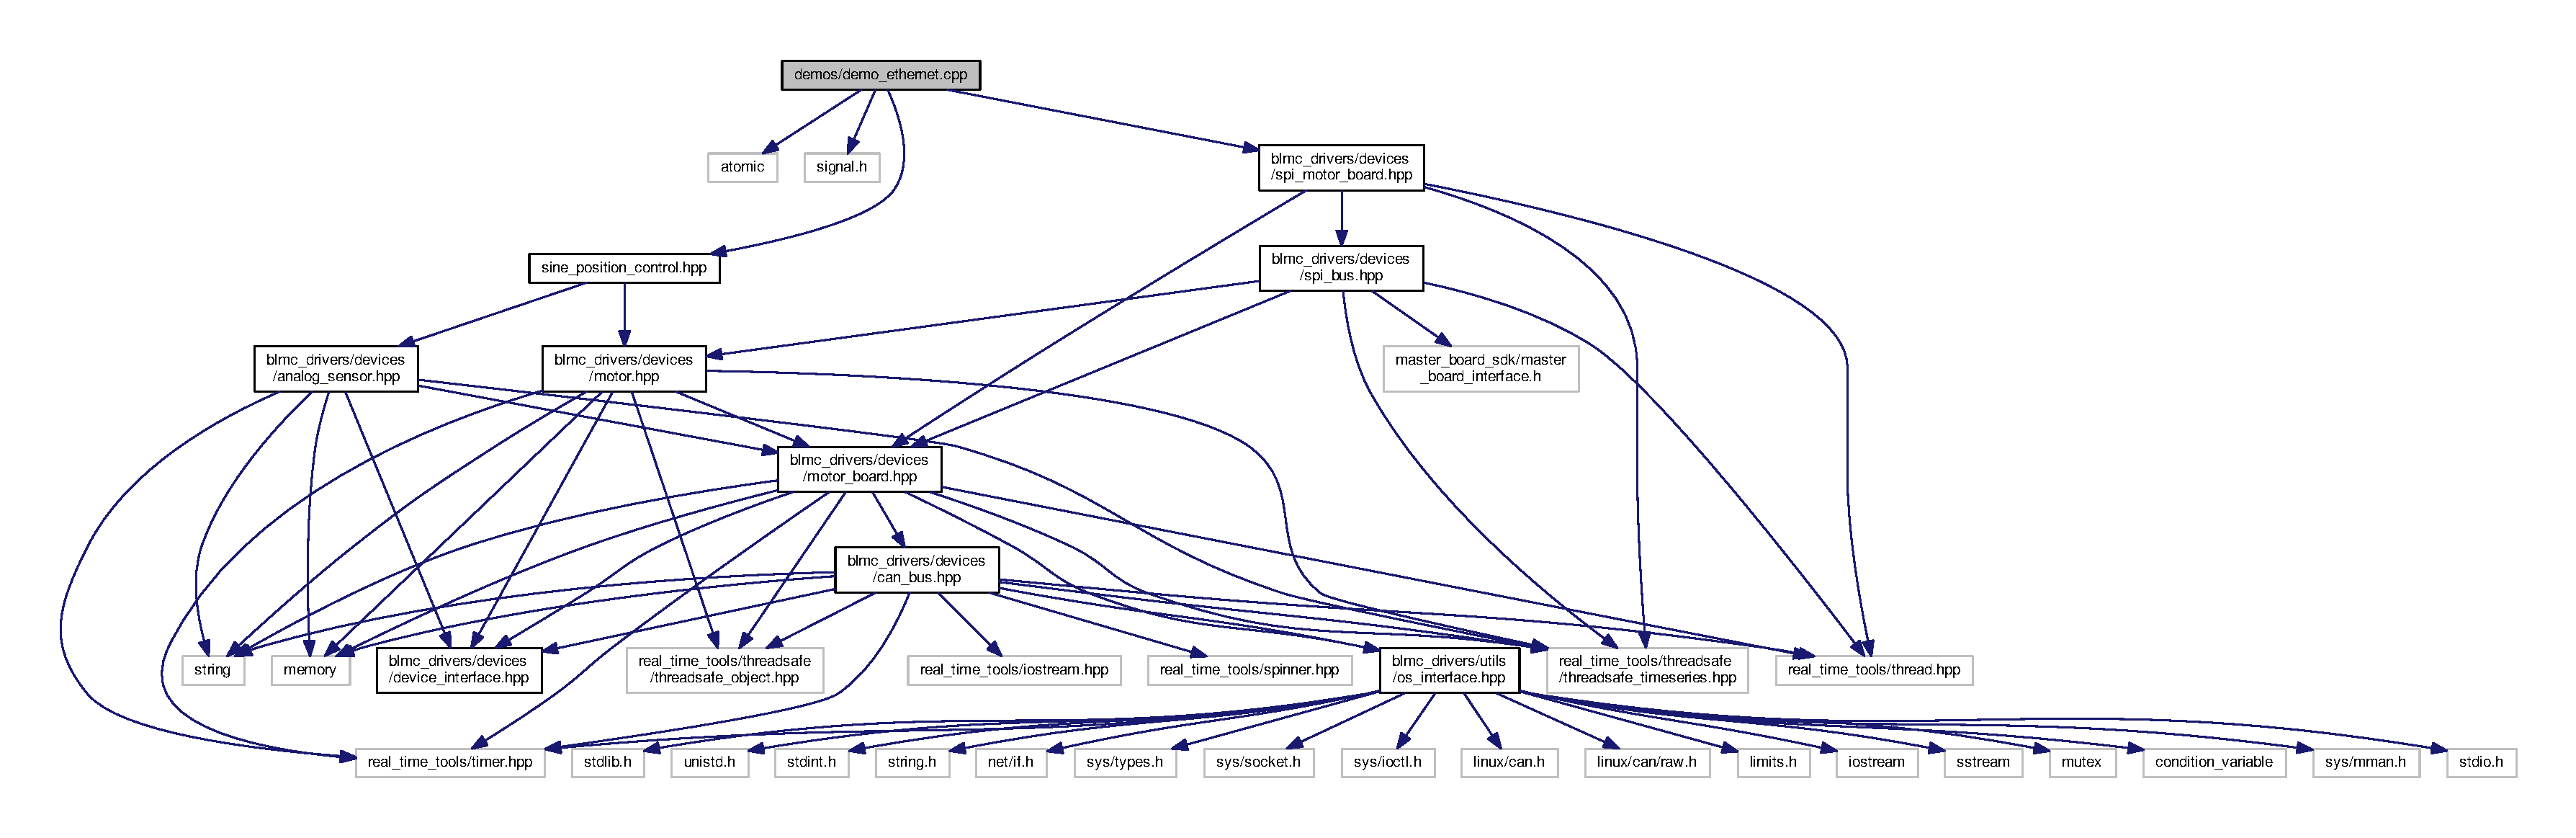
\includegraphics[width=350pt]{demo__ethernet_8cpp__incl}
\end{center}
\end{figure}
\subsection*{Functions}
\begin{DoxyCompactItemize}
\item 
std\+::atomic\+\_\+bool \hyperlink{demo__ethernet_8cpp_a37348e9dd6283af4127a90367a9482d1}{g\+\_\+stop\+\_\+demo} (false)\hypertarget{demo__ethernet_8cpp_a37348e9dd6283af4127a90367a9482d1}{}\label{demo__ethernet_8cpp_a37348e9dd6283af4127a90367a9482d1}

\begin{DoxyCompactList}\small\item\em This boolean is here to kill cleanly the application upon ctrl+c. \end{DoxyCompactList}\item 
void \hyperlink{demo__ethernet_8cpp_a3d51efaeecab2023836cefe28d4dcff4}{my\+\_\+handler} (int)
\begin{DoxyCompactList}\small\item\em This function is the callback upon a ctrl+c call from the terminal. \end{DoxyCompactList}\item 
int \hyperlink{demo__ethernet_8cpp_a3c04138a5bfe5d72780bb7e82a18e627}{main} (int argc, char $\ast$$\ast$argv)
\begin{DoxyCompactList}\small\item\em This is the main demo program. \end{DoxyCompactList}\end{DoxyCompactItemize}


\subsection{Detailed Description}
\begin{DoxyCopyright}{Copyright}
Copyright (c) 2018-\/2020, New York University and Max Planck Gesellschaft, License B\+S\+D-\/3-\/\+Clause 
\end{DoxyCopyright}


\subsection{Function Documentation}
\index{demo\+\_\+ethernet.\+cpp@{demo\+\_\+ethernet.\+cpp}!main@{main}}
\index{main@{main}!demo\+\_\+ethernet.\+cpp@{demo\+\_\+ethernet.\+cpp}}
\subsubsection[{\texorpdfstring{main(int argc, char $\ast$$\ast$argv)}{main(int argc, char **argv)}}]{\setlength{\rightskip}{0pt plus 5cm}int main (
\begin{DoxyParamCaption}
\item[{int}]{argc, }
\item[{char $\ast$$\ast$}]{argv}
\end{DoxyParamCaption}
)}\hypertarget{demo__ethernet_8cpp_a3c04138a5bfe5d72780bb7e82a18e627}{}\label{demo__ethernet_8cpp_a3c04138a5bfe5d72780bb7e82a18e627}


This is the main demo program. 


\begin{DoxyParams}{Parameters}
{\em argc} & \\
\hline
{\em argv} & \\
\hline
\end{DoxyParams}
\begin{DoxyReturn}{Returns}
int 
\end{DoxyReturn}
\index{demo\+\_\+ethernet.\+cpp@{demo\+\_\+ethernet.\+cpp}!my\+\_\+handler@{my\+\_\+handler}}
\index{my\+\_\+handler@{my\+\_\+handler}!demo\+\_\+ethernet.\+cpp@{demo\+\_\+ethernet.\+cpp}}
\subsubsection[{\texorpdfstring{my\+\_\+handler(int)}{my_handler(int)}}]{\setlength{\rightskip}{0pt plus 5cm}void my\+\_\+handler (
\begin{DoxyParamCaption}
\item[{int}]{}
\end{DoxyParamCaption}
)}\hypertarget{demo__ethernet_8cpp_a3d51efaeecab2023836cefe28d4dcff4}{}\label{demo__ethernet_8cpp_a3d51efaeecab2023836cefe28d4dcff4}


This function is the callback upon a ctrl+c call from the terminal. 


\begin{DoxyParams}{Parameters}
{\em s} & \\
\hline
\end{DoxyParams}

\hypertarget{demo__leg_8cpp}{}\section{demos/demo\+\_\+leg.cpp File Reference}
\label{demo__leg_8cpp}\index{demos/demo\+\_\+leg.\+cpp@{demos/demo\+\_\+leg.\+cpp}}
{\ttfamily \#include \char`\"{}real\+\_\+time\+\_\+tools/timer.\+hpp\char`\"{}}\\*
{\ttfamily \#include \char`\"{}real\+\_\+time\+\_\+tools/spinner.\+hpp\char`\"{}}\\*
{\ttfamily \#include $<$blmc\+\_\+drivers/devices/motor.\+hpp$>$}\\*
{\ttfamily \#include $<$blmc\+\_\+drivers/devices/analog\+\_\+sensor.\+hpp$>$}\\*
{\ttfamily \#include $<$blmc\+\_\+drivers/devices/leg.\+hpp$>$}\\*
{\ttfamily \#include $<$math.\+h$>$}\\*
{\ttfamily \#include $<$atomic$>$}\\*
{\ttfamily \#include $<$signal.\+h$>$}\\*
{\ttfamily \#include $<$pd\+\_\+control.\+hpp$>$}\\*
Include dependency graph for demo\+\_\+leg.\+cpp\+:
\nopagebreak
\begin{figure}[H]
\begin{center}
\leavevmode
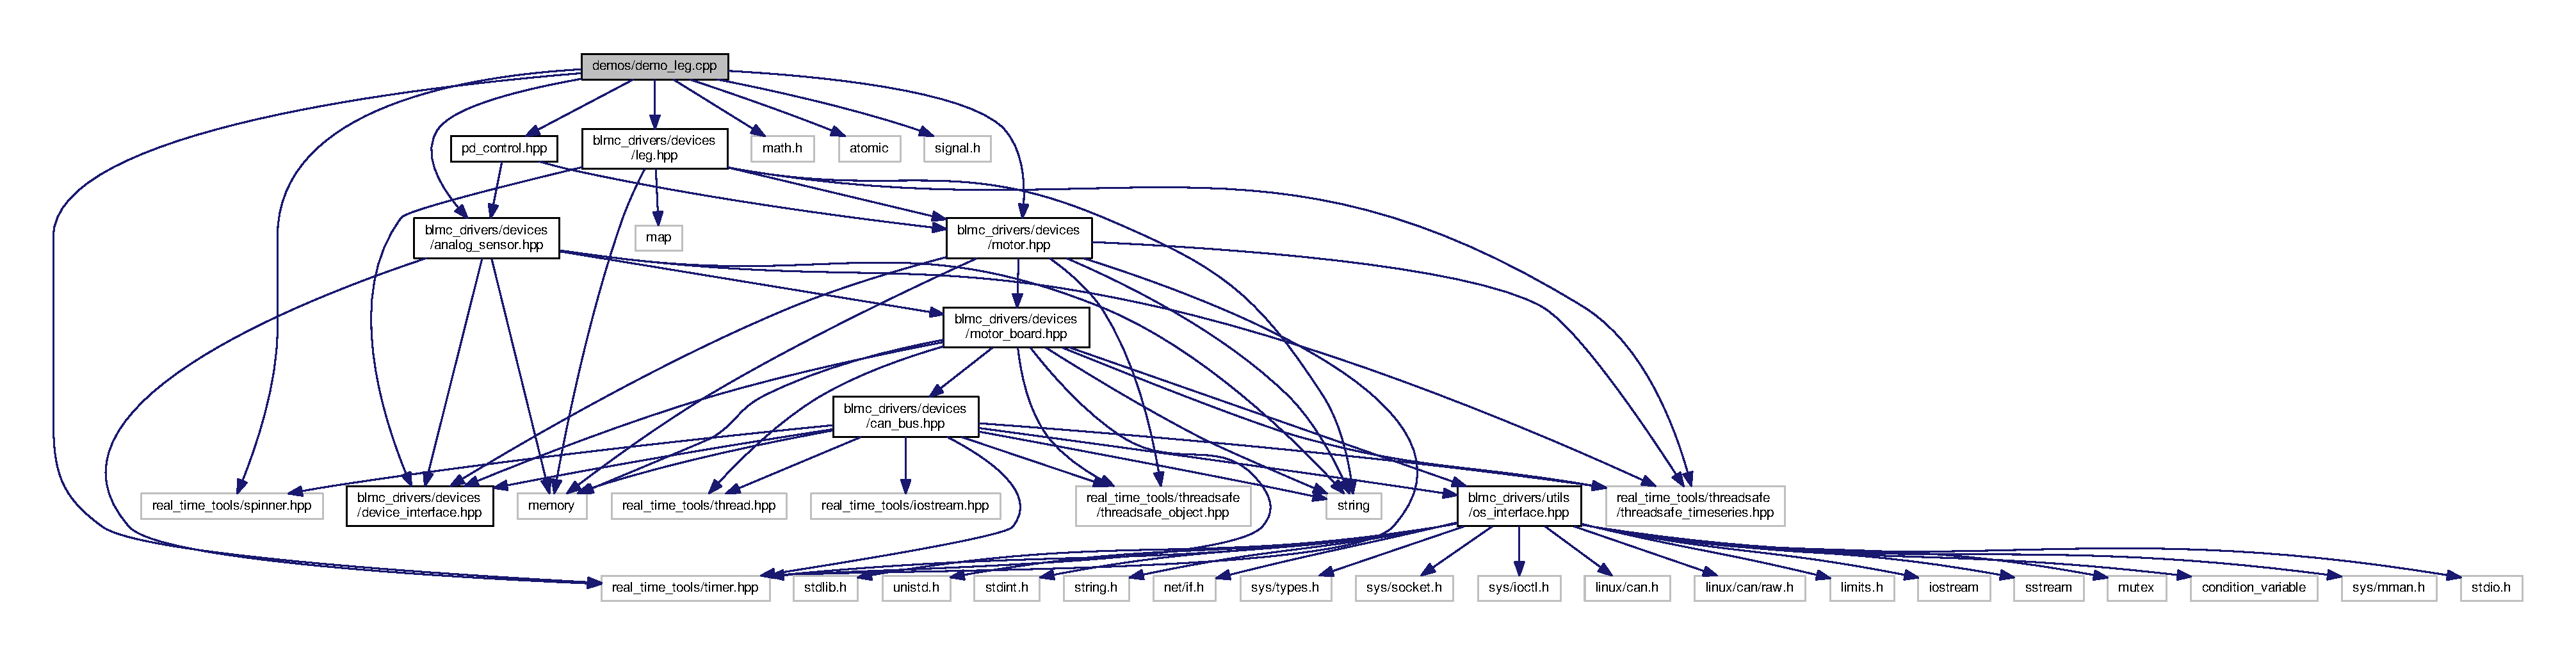
\includegraphics[width=350pt]{demo__leg_8cpp__incl}
\end{center}
\end{figure}
\subsection*{Classes}
\begin{DoxyCompactItemize}
\item 
class \hyperlink{classController}{Controller}
\begin{DoxyCompactList}\small\item\em This is a simple PD control on one motor and one slider. \end{DoxyCompactList}\item 
class \hyperlink{classLegController}{Leg\+Controller}
\begin{DoxyCompactList}\small\item\em Simple PD control on the leg. \end{DoxyCompactList}\end{DoxyCompactItemize}
\subsection*{Functions}
\begin{DoxyCompactItemize}
\item 
std\+::atomic\+\_\+bool \hyperlink{demo__leg_8cpp_a75d8b98fafbd2fb243e91c6164b114ce}{Stop\+Demos} (false)\hypertarget{demo__leg_8cpp_a75d8b98fafbd2fb243e91c6164b114ce}{}\label{demo__leg_8cpp_a75d8b98fafbd2fb243e91c6164b114ce}

\begin{DoxyCompactList}\small\item\em This boolean is here to kill cleanly the application upon ctrl+c. \end{DoxyCompactList}\item 
void \hyperlink{demo__leg_8cpp_a3d51efaeecab2023836cefe28d4dcff4}{my\+\_\+handler} (int)
\begin{DoxyCompactList}\small\item\em This function is the callback upon a ctrl+c call from the terminal. \end{DoxyCompactList}\item 
int {\bfseries main} (int, char $\ast$$\ast$)\hypertarget{demo__leg_8cpp_a2c3f6775325c30275d11c6abee2db6a0}{}\label{demo__leg_8cpp_a2c3f6775325c30275d11c6abee2db6a0}

\end{DoxyCompactItemize}


\subsection{Detailed Description}
\begin{DoxyCopyright}{Copyright}
Copyright (c) 2018-\/2020, New York University and Max Planck Gesellschaft, License B\+S\+D-\/3-\/\+Clause 
\end{DoxyCopyright}


\subsection{Function Documentation}
\index{demo\+\_\+leg.\+cpp@{demo\+\_\+leg.\+cpp}!my\+\_\+handler@{my\+\_\+handler}}
\index{my\+\_\+handler@{my\+\_\+handler}!demo\+\_\+leg.\+cpp@{demo\+\_\+leg.\+cpp}}
\subsubsection[{\texorpdfstring{my\+\_\+handler(int)}{my_handler(int)}}]{\setlength{\rightskip}{0pt plus 5cm}void my\+\_\+handler (
\begin{DoxyParamCaption}
\item[{int}]{}
\end{DoxyParamCaption}
)}\hypertarget{demo__leg_8cpp_a3d51efaeecab2023836cefe28d4dcff4}{}\label{demo__leg_8cpp_a3d51efaeecab2023836cefe28d4dcff4}


This function is the callback upon a ctrl+c call from the terminal. 


\begin{DoxyParams}{Parameters}
{\em s} & \\
\hline
\end{DoxyParams}

\hypertarget{demo__sine__position__1__motor_8cpp}{}\section{demos/demo\+\_\+sine\+\_\+position\+\_\+1\+\_\+motor.cpp File Reference}
\label{demo__sine__position__1__motor_8cpp}\index{demos/demo\+\_\+sine\+\_\+position\+\_\+1\+\_\+motor.\+cpp@{demos/demo\+\_\+sine\+\_\+position\+\_\+1\+\_\+motor.\+cpp}}
{\ttfamily \#include $<$atomic$>$}\\*
{\ttfamily \#include $<$signal.\+h$>$}\\*
{\ttfamily \#include \char`\"{}sine\+\_\+position\+\_\+control.\+hpp\char`\"{}}\\*
Include dependency graph for demo\+\_\+sine\+\_\+position\+\_\+1\+\_\+motor.\+cpp\+:
\nopagebreak
\begin{figure}[H]
\begin{center}
\leavevmode
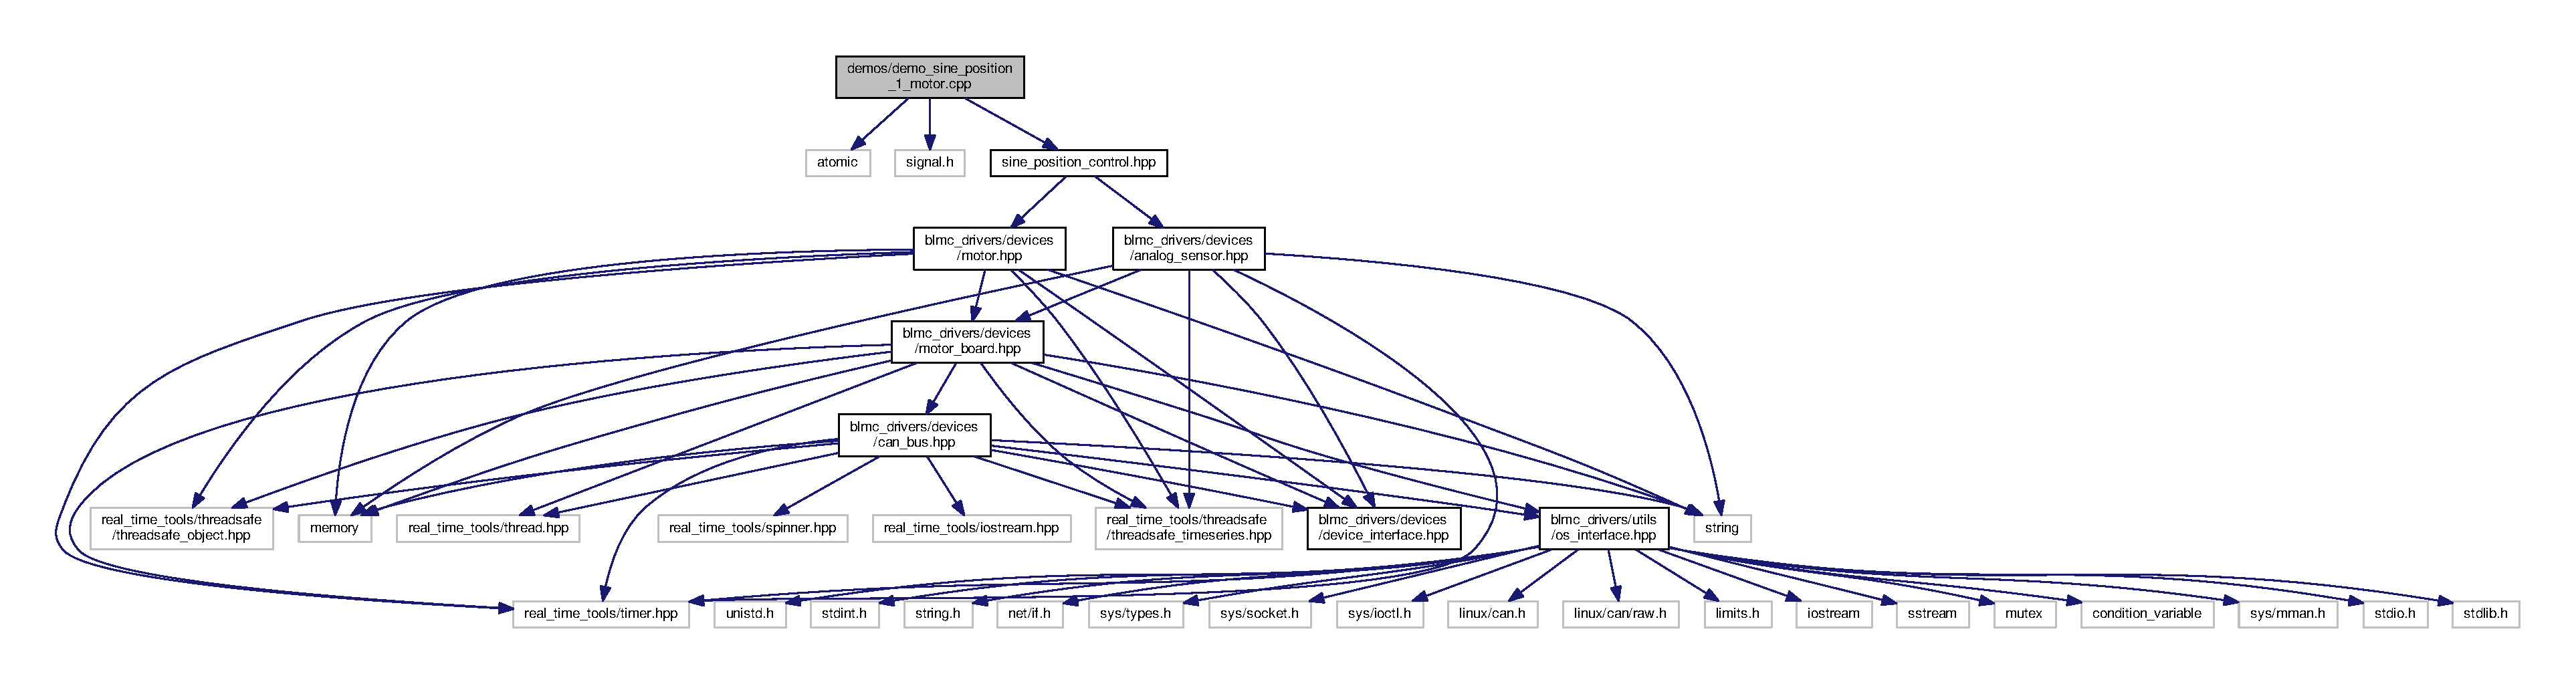
\includegraphics[width=350pt]{demo__sine__position__1__motor_8cpp__incl}
\end{center}
\end{figure}
\subsection*{Functions}
\begin{DoxyCompactItemize}
\item 
std\+::atomic\+\_\+bool \hyperlink{demo__sine__position__1__motor_8cpp_a75d8b98fafbd2fb243e91c6164b114ce}{Stop\+Demos} (false)\hypertarget{demo__sine__position__1__motor_8cpp_a75d8b98fafbd2fb243e91c6164b114ce}{}\label{demo__sine__position__1__motor_8cpp_a75d8b98fafbd2fb243e91c6164b114ce}

\begin{DoxyCompactList}\small\item\em This boolean is here to kill cleanly the application upon ctrl+c. \end{DoxyCompactList}\item 
void \hyperlink{demo__sine__position__1__motor_8cpp_a3d51efaeecab2023836cefe28d4dcff4}{my\+\_\+handler} (int)
\begin{DoxyCompactList}\small\item\em This function is the callback upon a ctrl+c call from the terminal. \end{DoxyCompactList}\item 
int \hyperlink{demo__sine__position__1__motor_8cpp_a2c3f6775325c30275d11c6abee2db6a0}{main} (int, char $\ast$$\ast$)
\begin{DoxyCompactList}\small\item\em This is the main demo program. \end{DoxyCompactList}\end{DoxyCompactItemize}


\subsection{Detailed Description}
\begin{DoxyCopyright}{Copyright}
Copyright (c) 2018-\/2020, New York University and Max Planck Gesellschaft, License B\+S\+D-\/3-\/\+Clause 
\end{DoxyCopyright}


\subsection{Function Documentation}
\index{demo\+\_\+sine\+\_\+position\+\_\+1\+\_\+motor.\+cpp@{demo\+\_\+sine\+\_\+position\+\_\+1\+\_\+motor.\+cpp}!main@{main}}
\index{main@{main}!demo\+\_\+sine\+\_\+position\+\_\+1\+\_\+motor.\+cpp@{demo\+\_\+sine\+\_\+position\+\_\+1\+\_\+motor.\+cpp}}
\subsubsection[{\texorpdfstring{main(int, char $\ast$$\ast$)}{main(int, char **)}}]{\setlength{\rightskip}{0pt plus 5cm}int main (
\begin{DoxyParamCaption}
\item[{int}]{, }
\item[{char $\ast$$\ast$}]{}
\end{DoxyParamCaption}
)}\hypertarget{demo__sine__position__1__motor_8cpp_a2c3f6775325c30275d11c6abee2db6a0}{}\label{demo__sine__position__1__motor_8cpp_a2c3f6775325c30275d11c6abee2db6a0}


This is the main demo program. 


\begin{DoxyParams}{Parameters}
{\em argc} & \\
\hline
{\em argv} & \\
\hline
\end{DoxyParams}
\begin{DoxyReturn}{Returns}
int 
\end{DoxyReturn}
\index{demo\+\_\+sine\+\_\+position\+\_\+1\+\_\+motor.\+cpp@{demo\+\_\+sine\+\_\+position\+\_\+1\+\_\+motor.\+cpp}!my\+\_\+handler@{my\+\_\+handler}}
\index{my\+\_\+handler@{my\+\_\+handler}!demo\+\_\+sine\+\_\+position\+\_\+1\+\_\+motor.\+cpp@{demo\+\_\+sine\+\_\+position\+\_\+1\+\_\+motor.\+cpp}}
\subsubsection[{\texorpdfstring{my\+\_\+handler(int)}{my_handler(int)}}]{\setlength{\rightskip}{0pt plus 5cm}void my\+\_\+handler (
\begin{DoxyParamCaption}
\item[{int}]{}
\end{DoxyParamCaption}
)}\hypertarget{demo__sine__position__1__motor_8cpp_a3d51efaeecab2023836cefe28d4dcff4}{}\label{demo__sine__position__1__motor_8cpp_a3d51efaeecab2023836cefe28d4dcff4}


This function is the callback upon a ctrl+c call from the terminal. 


\begin{DoxyParams}{Parameters}
{\em s} & \\
\hline
\end{DoxyParams}

\hypertarget{demo__sine__torque__1__motor_8cpp}{}\section{demos/demo\+\_\+sine\+\_\+torque\+\_\+1\+\_\+motor.cpp File Reference}
\label{demo__sine__torque__1__motor_8cpp}\index{demos/demo\+\_\+sine\+\_\+torque\+\_\+1\+\_\+motor.\+cpp@{demos/demo\+\_\+sine\+\_\+torque\+\_\+1\+\_\+motor.\+cpp}}
{\ttfamily \#include $<$atomic$>$}\\*
{\ttfamily \#include $<$signal.\+h$>$}\\*
{\ttfamily \#include \char`\"{}sine\+\_\+torque\+\_\+control.\+hpp\char`\"{}}\\*
Include dependency graph for demo\+\_\+sine\+\_\+torque\+\_\+1\+\_\+motor.\+cpp\+:
\nopagebreak
\begin{figure}[H]
\begin{center}
\leavevmode
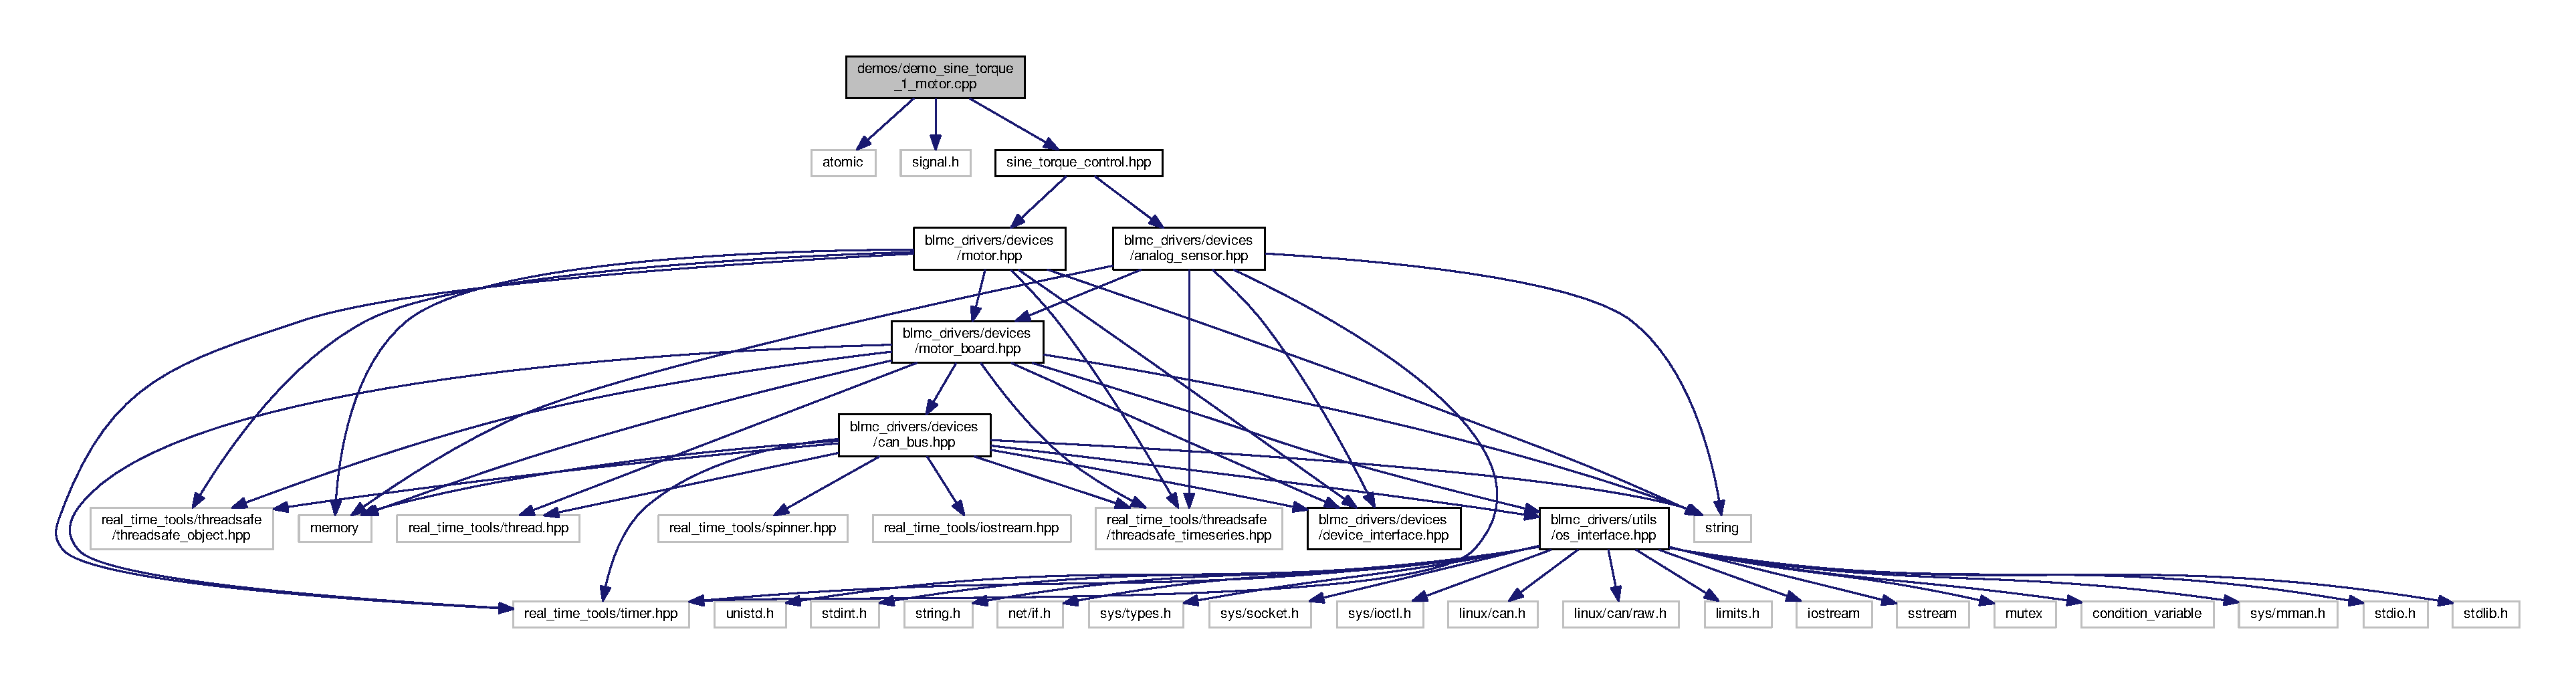
\includegraphics[width=350pt]{demo__sine__torque__1__motor_8cpp__incl}
\end{center}
\end{figure}
\subsection*{Functions}
\begin{DoxyCompactItemize}
\item 
std\+::atomic\+\_\+bool \hyperlink{demo__sine__torque__1__motor_8cpp_a75d8b98fafbd2fb243e91c6164b114ce}{Stop\+Demos} (false)\hypertarget{demo__sine__torque__1__motor_8cpp_a75d8b98fafbd2fb243e91c6164b114ce}{}\label{demo__sine__torque__1__motor_8cpp_a75d8b98fafbd2fb243e91c6164b114ce}

\begin{DoxyCompactList}\small\item\em This boolean is here to kill cleanly the application upon ctrl+c. \end{DoxyCompactList}\item 
void \hyperlink{demo__sine__torque__1__motor_8cpp_a3d51efaeecab2023836cefe28d4dcff4}{my\+\_\+handler} (int)
\begin{DoxyCompactList}\small\item\em This function is the callback upon a ctrl+c call from the terminal. \end{DoxyCompactList}\item 
int \hyperlink{demo__sine__torque__1__motor_8cpp_a2c3f6775325c30275d11c6abee2db6a0}{main} (int, char $\ast$$\ast$)
\begin{DoxyCompactList}\small\item\em This is the main demo program. \end{DoxyCompactList}\end{DoxyCompactItemize}


\subsection{Detailed Description}
\begin{DoxyCopyright}{Copyright}
Copyright (c) 2018-\/2020, New York University and Max Planck Gesellschaft, License B\+S\+D-\/3-\/\+Clause 
\end{DoxyCopyright}


\subsection{Function Documentation}
\index{demo\+\_\+sine\+\_\+torque\+\_\+1\+\_\+motor.\+cpp@{demo\+\_\+sine\+\_\+torque\+\_\+1\+\_\+motor.\+cpp}!main@{main}}
\index{main@{main}!demo\+\_\+sine\+\_\+torque\+\_\+1\+\_\+motor.\+cpp@{demo\+\_\+sine\+\_\+torque\+\_\+1\+\_\+motor.\+cpp}}
\subsubsection[{\texorpdfstring{main(int, char $\ast$$\ast$)}{main(int, char **)}}]{\setlength{\rightskip}{0pt plus 5cm}int main (
\begin{DoxyParamCaption}
\item[{int}]{, }
\item[{char $\ast$$\ast$}]{}
\end{DoxyParamCaption}
)}\hypertarget{demo__sine__torque__1__motor_8cpp_a2c3f6775325c30275d11c6abee2db6a0}{}\label{demo__sine__torque__1__motor_8cpp_a2c3f6775325c30275d11c6abee2db6a0}


This is the main demo program. 


\begin{DoxyParams}{Parameters}
{\em argc} & \\
\hline
{\em argv} & \\
\hline
\end{DoxyParams}
\begin{DoxyReturn}{Returns}
int 
\end{DoxyReturn}
\index{demo\+\_\+sine\+\_\+torque\+\_\+1\+\_\+motor.\+cpp@{demo\+\_\+sine\+\_\+torque\+\_\+1\+\_\+motor.\+cpp}!my\+\_\+handler@{my\+\_\+handler}}
\index{my\+\_\+handler@{my\+\_\+handler}!demo\+\_\+sine\+\_\+torque\+\_\+1\+\_\+motor.\+cpp@{demo\+\_\+sine\+\_\+torque\+\_\+1\+\_\+motor.\+cpp}}
\subsubsection[{\texorpdfstring{my\+\_\+handler(int)}{my_handler(int)}}]{\setlength{\rightskip}{0pt plus 5cm}void my\+\_\+handler (
\begin{DoxyParamCaption}
\item[{int}]{}
\end{DoxyParamCaption}
)}\hypertarget{demo__sine__torque__1__motor_8cpp_a3d51efaeecab2023836cefe28d4dcff4}{}\label{demo__sine__torque__1__motor_8cpp_a3d51efaeecab2023836cefe28d4dcff4}


This function is the callback upon a ctrl+c call from the terminal. 


\begin{DoxyParams}{Parameters}
{\em s} & \\
\hline
\end{DoxyParams}

\hypertarget{demo__single__board_8cpp}{}\section{demos/demo\+\_\+single\+\_\+board.cpp File Reference}
\label{demo__single__board_8cpp}\index{demos/demo\+\_\+single\+\_\+board.\+cpp@{demos/demo\+\_\+single\+\_\+board.\+cpp}}
{\ttfamily \#include $<$atomic$>$}\\*
{\ttfamily \#include $<$signal.\+h$>$}\\*
{\ttfamily \#include \char`\"{}pd\+\_\+control.\+hpp\char`\"{}}\\*
Include dependency graph for demo\+\_\+single\+\_\+board.\+cpp\+:
\nopagebreak
\begin{figure}[H]
\begin{center}
\leavevmode
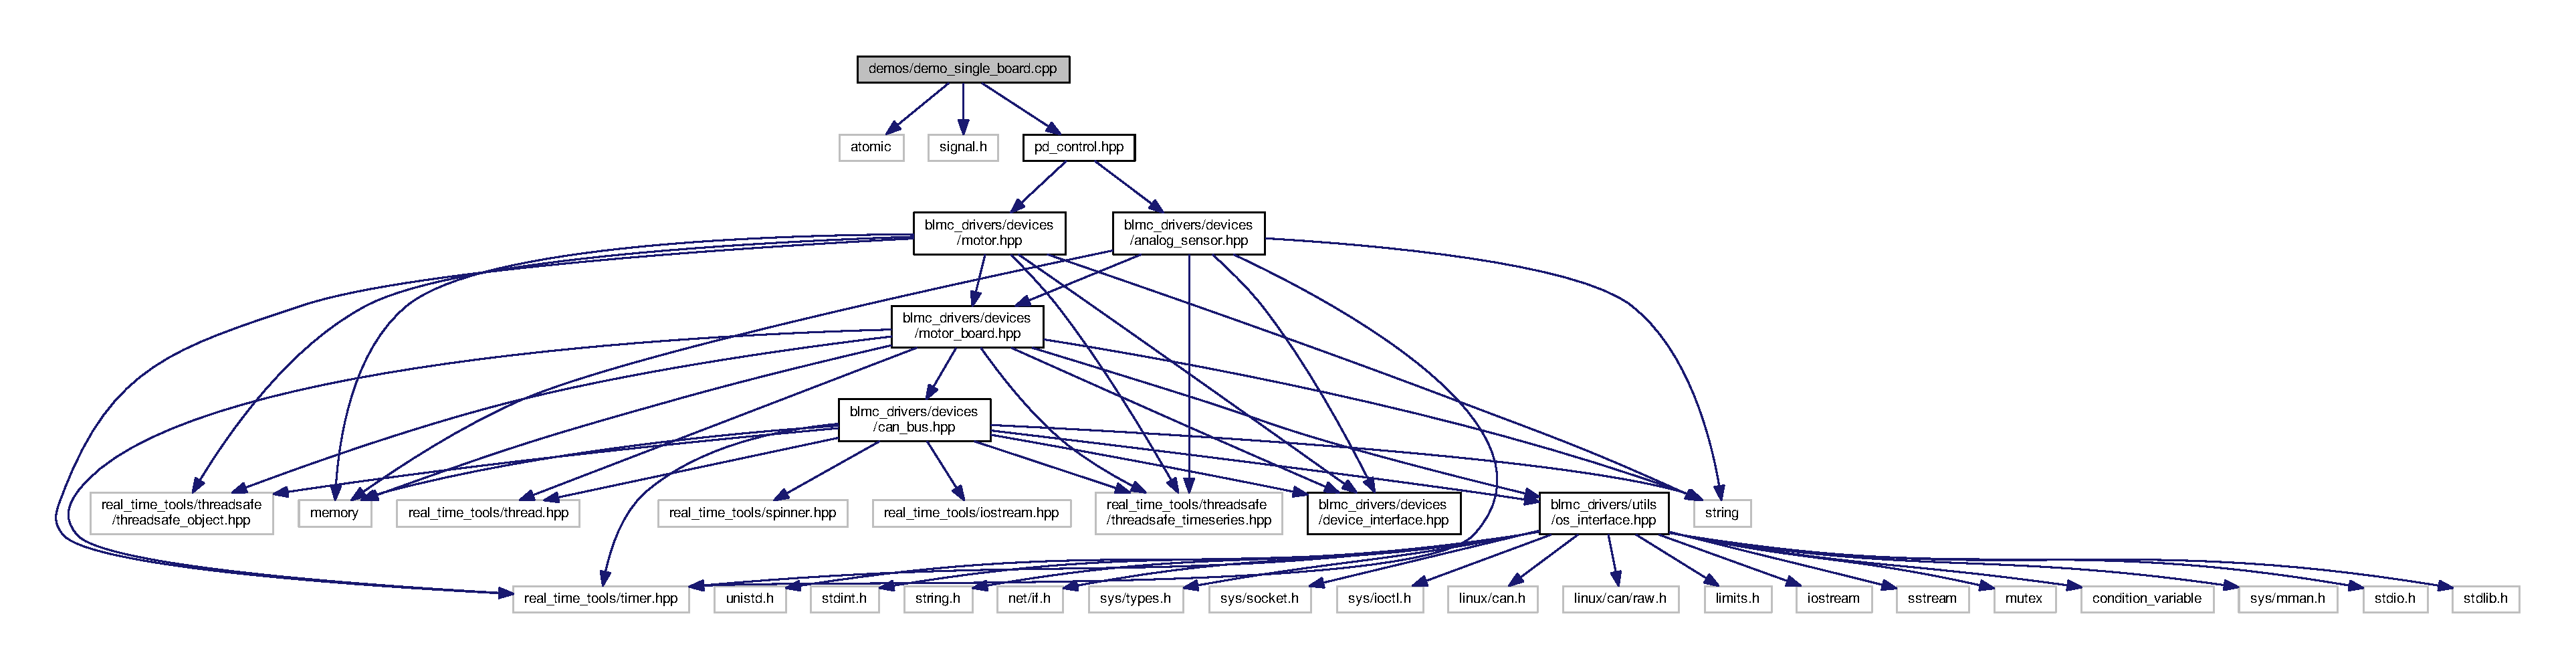
\includegraphics[width=350pt]{demo__single__board_8cpp__incl}
\end{center}
\end{figure}
\subsection*{Functions}
\begin{DoxyCompactItemize}
\item 
std\+::atomic\+\_\+bool \hyperlink{demo__single__board_8cpp_a75d8b98fafbd2fb243e91c6164b114ce}{Stop\+Demos} (false)\hypertarget{demo__single__board_8cpp_a75d8b98fafbd2fb243e91c6164b114ce}{}\label{demo__single__board_8cpp_a75d8b98fafbd2fb243e91c6164b114ce}

\begin{DoxyCompactList}\small\item\em This boolean is here to kill cleanly the application upon ctrl+c. \end{DoxyCompactList}\item 
void \hyperlink{demo__single__board_8cpp_a3d51efaeecab2023836cefe28d4dcff4}{my\+\_\+handler} (int)
\begin{DoxyCompactList}\small\item\em This function is the callback upon a ctrl+c call from the terminal. \end{DoxyCompactList}\item 
int \hyperlink{demo__single__board_8cpp_a2c3f6775325c30275d11c6abee2db6a0}{main} (int, char $\ast$$\ast$)
\begin{DoxyCompactList}\small\item\em This is the main demo program. \end{DoxyCompactList}\end{DoxyCompactItemize}


\subsection{Detailed Description}
\begin{DoxyCopyright}{Copyright}
Copyright (c) 2018-\/2020, New York University and Max Planck Gesellschaft, License B\+S\+D-\/3-\/\+Clause 
\end{DoxyCopyright}


\subsection{Function Documentation}
\index{demo\+\_\+single\+\_\+board.\+cpp@{demo\+\_\+single\+\_\+board.\+cpp}!main@{main}}
\index{main@{main}!demo\+\_\+single\+\_\+board.\+cpp@{demo\+\_\+single\+\_\+board.\+cpp}}
\subsubsection[{\texorpdfstring{main(int, char $\ast$$\ast$)}{main(int, char **)}}]{\setlength{\rightskip}{0pt plus 5cm}int main (
\begin{DoxyParamCaption}
\item[{int}]{, }
\item[{char $\ast$$\ast$}]{}
\end{DoxyParamCaption}
)}\hypertarget{demo__single__board_8cpp_a2c3f6775325c30275d11c6abee2db6a0}{}\label{demo__single__board_8cpp_a2c3f6775325c30275d11c6abee2db6a0}


This is the main demo program. 


\begin{DoxyParams}{Parameters}
{\em argc} & \\
\hline
{\em argv} & \\
\hline
\end{DoxyParams}
\begin{DoxyReturn}{Returns}
int 
\end{DoxyReturn}
\index{demo\+\_\+single\+\_\+board.\+cpp@{demo\+\_\+single\+\_\+board.\+cpp}!my\+\_\+handler@{my\+\_\+handler}}
\index{my\+\_\+handler@{my\+\_\+handler}!demo\+\_\+single\+\_\+board.\+cpp@{demo\+\_\+single\+\_\+board.\+cpp}}
\subsubsection[{\texorpdfstring{my\+\_\+handler(int)}{my_handler(int)}}]{\setlength{\rightskip}{0pt plus 5cm}void my\+\_\+handler (
\begin{DoxyParamCaption}
\item[{int}]{}
\end{DoxyParamCaption}
)}\hypertarget{demo__single__board_8cpp_a3d51efaeecab2023836cefe28d4dcff4}{}\label{demo__single__board_8cpp_a3d51efaeecab2023836cefe28d4dcff4}


This function is the callback upon a ctrl+c call from the terminal. 


\begin{DoxyParams}{Parameters}
{\em s} & \\
\hline
\end{DoxyParams}

\hypertarget{pd__control_8cpp}{}\section{demos/pd\+\_\+control.cpp File Reference}
\label{pd__control_8cpp}\index{demos/pd\+\_\+control.\+cpp@{demos/pd\+\_\+control.\+cpp}}
{\ttfamily \#include \char`\"{}real\+\_\+time\+\_\+tools/timer.\+hpp\char`\"{}}\\*
{\ttfamily \#include \char`\"{}real\+\_\+time\+\_\+tools/spinner.\+hpp\char`\"{}}\\*
{\ttfamily \#include \char`\"{}pd\+\_\+control.\+hpp\char`\"{}}\\*
Include dependency graph for pd\+\_\+control.\+cpp\+:
\nopagebreak
\begin{figure}[H]
\begin{center}
\leavevmode
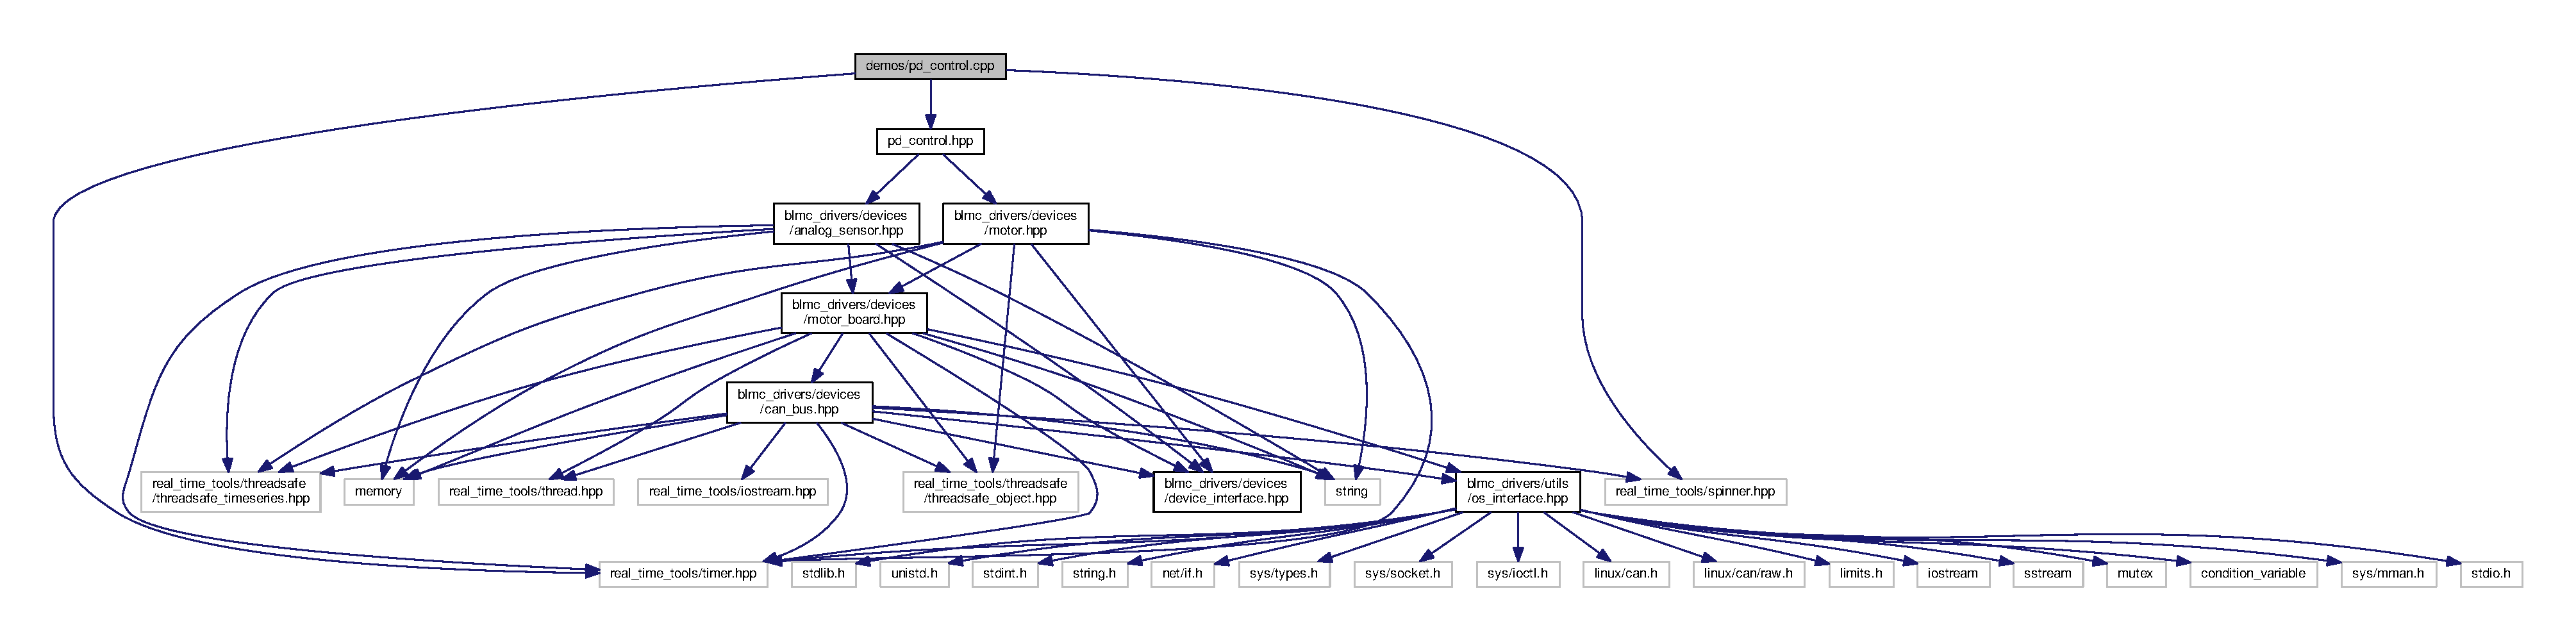
\includegraphics[width=350pt]{pd__control_8cpp__incl}
\end{center}
\end{figure}
\subsection*{Namespaces}
\begin{DoxyCompactItemize}
\item 
 \hyperlink{namespaceblmc__drivers}{blmc\+\_\+drivers}
\begin{DoxyCompactList}\small\item\em This namespace is the standard namespace of the package. \end{DoxyCompactList}\end{DoxyCompactItemize}


\subsection{Detailed Description}
\begin{DoxyCopyright}{Copyright}
Copyright (c) 2018-\/2020, New York University and Max Planck Gesellschaft, License B\+S\+D-\/3-\/\+Clause 
\end{DoxyCopyright}

\hypertarget{pd__control_8hpp}{}\section{demos/pd\+\_\+control.hpp File Reference}
\label{pd__control_8hpp}\index{demos/pd\+\_\+control.\+hpp@{demos/pd\+\_\+control.\+hpp}}
{\ttfamily \#include \char`\"{}blmc\+\_\+drivers/devices/motor.\+hpp\char`\"{}}\\*
{\ttfamily \#include \char`\"{}blmc\+\_\+drivers/devices/analog\+\_\+sensor.\+hpp\char`\"{}}\\*
Include dependency graph for pd\+\_\+control.\+hpp\+:
\nopagebreak
\begin{figure}[H]
\begin{center}
\leavevmode
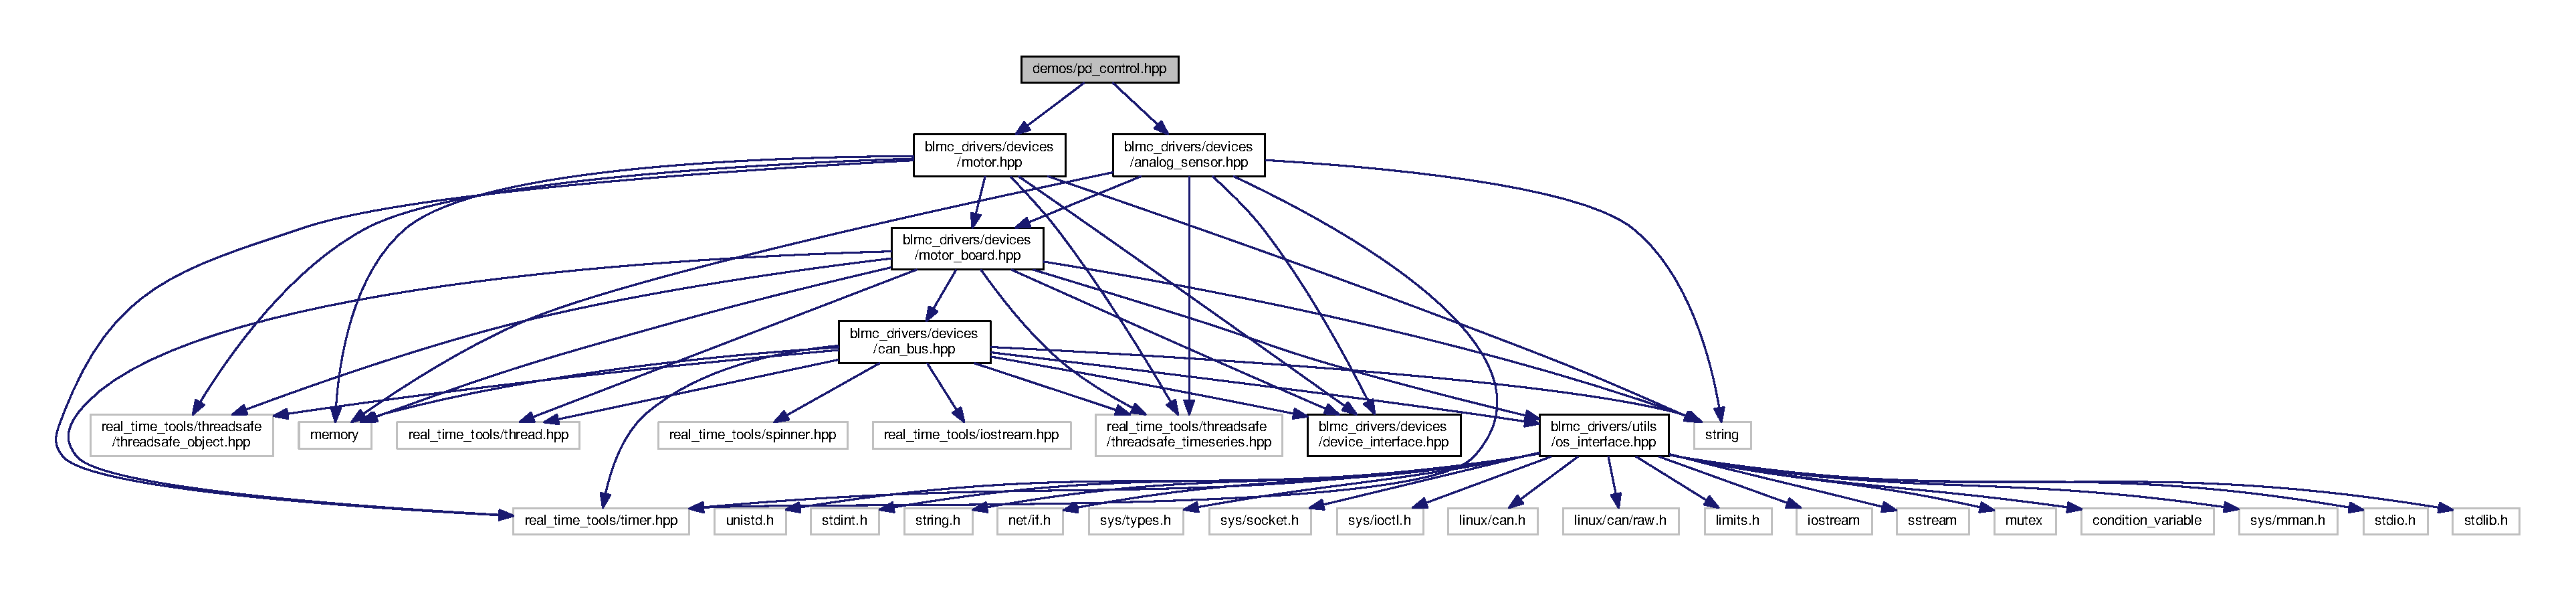
\includegraphics[width=350pt]{pd__control_8hpp__incl}
\end{center}
\end{figure}
This graph shows which files directly or indirectly include this file\+:
\nopagebreak
\begin{figure}[H]
\begin{center}
\leavevmode
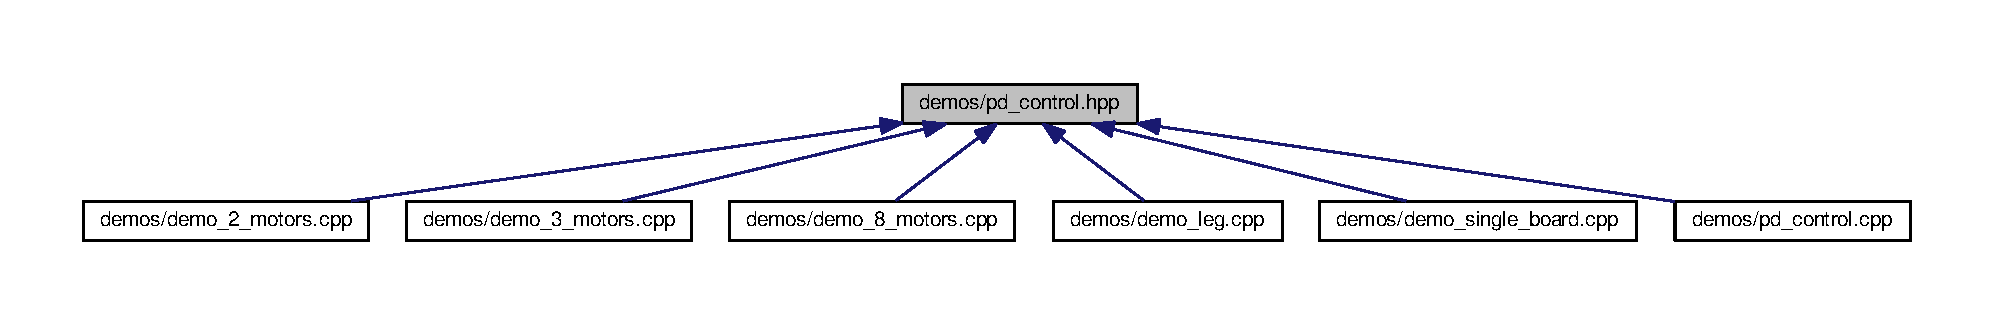
\includegraphics[width=350pt]{pd__control_8hpp__dep__incl}
\end{center}
\end{figure}
\subsection*{Classes}
\begin{DoxyCompactItemize}
\item 
class \hyperlink{classblmc__drivers_1_1PDController}{blmc\+\_\+drivers\+::\+P\+D\+Controller}
\begin{DoxyCompactList}\small\item\em This is a basic PD controller to be used in the demos of this package. \end{DoxyCompactList}\end{DoxyCompactItemize}
\subsection*{Namespaces}
\begin{DoxyCompactItemize}
\item 
 \hyperlink{namespaceblmc__drivers}{blmc\+\_\+drivers}
\begin{DoxyCompactList}\small\item\em This namespace is the standard namespace of the package. \end{DoxyCompactList}\end{DoxyCompactItemize}
\subsection*{Typedefs}
\begin{DoxyCompactItemize}
\item 
typedef std\+::shared\+\_\+ptr$<$ \hyperlink{classblmc__drivers_1_1AnalogSensor}{blmc\+\_\+drivers\+::\+Analog\+Sensor} $>$ \hyperlink{namespaceblmc__drivers_a1eb492ab42b913d5bcc21d53ba7185ba}{blmc\+\_\+drivers\+::\+Slider\+\_\+ptr}\hypertarget{namespaceblmc__drivers_a1eb492ab42b913d5bcc21d53ba7185ba}{}\label{namespaceblmc__drivers_a1eb492ab42b913d5bcc21d53ba7185ba}

\begin{DoxyCompactList}\small\item\em This is a simple shortcut. \end{DoxyCompactList}\item 
typedef std\+::pair$<$ Safe\+Motor\+\_\+ptr, Slider\+\_\+ptr $>$ \hyperlink{namespaceblmc__drivers_a134270c90d29a9a28b64ab0e5f7158f7}{blmc\+\_\+drivers\+::\+Pair\+Motor\+Slider}\hypertarget{namespaceblmc__drivers_a134270c90d29a9a28b64ab0e5f7158f7}{}\label{namespaceblmc__drivers_a134270c90d29a9a28b64ab0e5f7158f7}

\begin{DoxyCompactList}\small\item\em This is a simple shortcut. \end{DoxyCompactList}\end{DoxyCompactItemize}


\subsection{Detailed Description}
\begin{DoxyCopyright}{Copyright}
Copyright (c) 2018-\/2020, New York University and Max Planck Gesellschaft, License B\+S\+D-\/3-\/\+Clause 
\end{DoxyCopyright}

\hypertarget{sine__position__control_8cpp}{}\section{demos/sine\+\_\+position\+\_\+control.cpp File Reference}
\label{sine__position__control_8cpp}\index{demos/sine\+\_\+position\+\_\+control.\+cpp@{demos/sine\+\_\+position\+\_\+control.\+cpp}}
{\ttfamily \#include $<$fstream$>$}\\*
{\ttfamily \#include \char`\"{}real\+\_\+time\+\_\+tools/timer.\+hpp\char`\"{}}\\*
{\ttfamily \#include \char`\"{}real\+\_\+time\+\_\+tools/spinner.\+hpp\char`\"{}}\\*
{\ttfamily \#include \char`\"{}sine\+\_\+position\+\_\+control.\+hpp\char`\"{}}\\*
Include dependency graph for sine\+\_\+position\+\_\+control.\+cpp\+:
\nopagebreak
\begin{figure}[H]
\begin{center}
\leavevmode
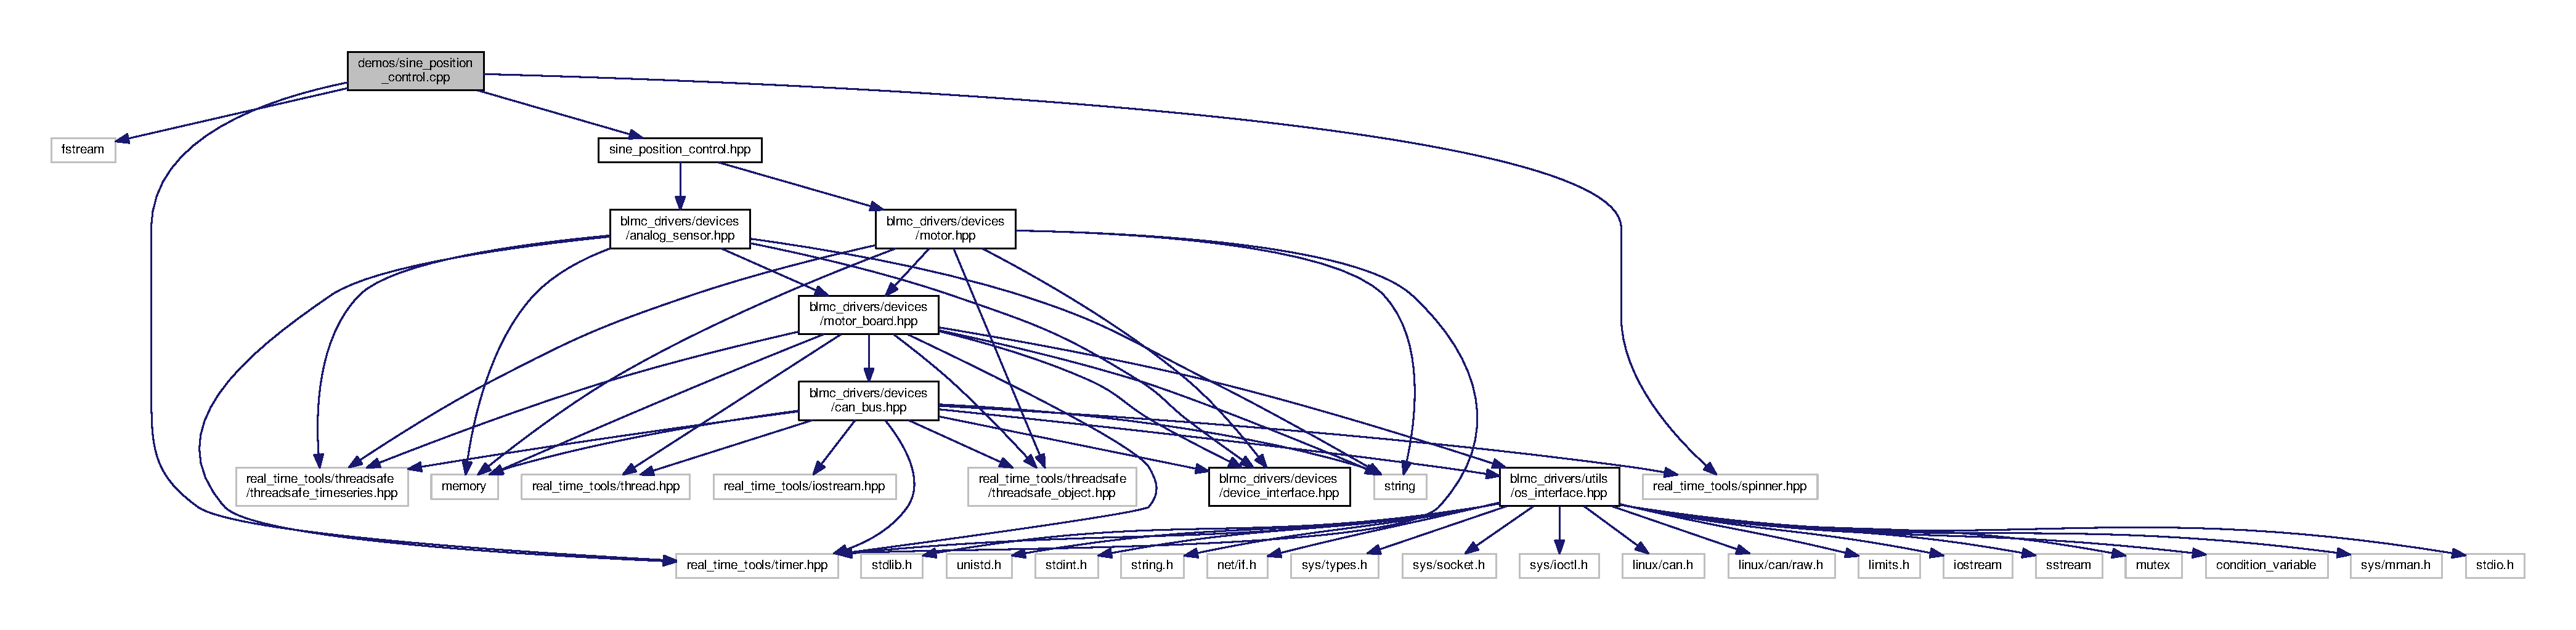
\includegraphics[width=350pt]{sine__position__control_8cpp__incl}
\end{center}
\end{figure}
\subsection*{Namespaces}
\begin{DoxyCompactItemize}
\item 
 \hyperlink{namespaceblmc__drivers}{blmc\+\_\+drivers}
\begin{DoxyCompactList}\small\item\em This namespace is the standard namespace of the package. \end{DoxyCompactList}\end{DoxyCompactItemize}


\subsection{Detailed Description}
\begin{DoxyCopyright}{Copyright}
Copyright (c) 2018-\/2020, New York University and Max Planck Gesellschaft, License B\+S\+D-\/3-\/\+Clause 
\end{DoxyCopyright}

\hypertarget{sine__position__control_8hpp}{}\section{demos/sine\+\_\+position\+\_\+control.hpp File Reference}
\label{sine__position__control_8hpp}\index{demos/sine\+\_\+position\+\_\+control.\+hpp@{demos/sine\+\_\+position\+\_\+control.\+hpp}}
{\ttfamily \#include \char`\"{}blmc\+\_\+drivers/devices/motor.\+hpp\char`\"{}}\\*
{\ttfamily \#include \char`\"{}blmc\+\_\+drivers/devices/analog\+\_\+sensor.\+hpp\char`\"{}}\\*
Include dependency graph for sine\+\_\+position\+\_\+control.\+hpp\+:
\nopagebreak
\begin{figure}[H]
\begin{center}
\leavevmode
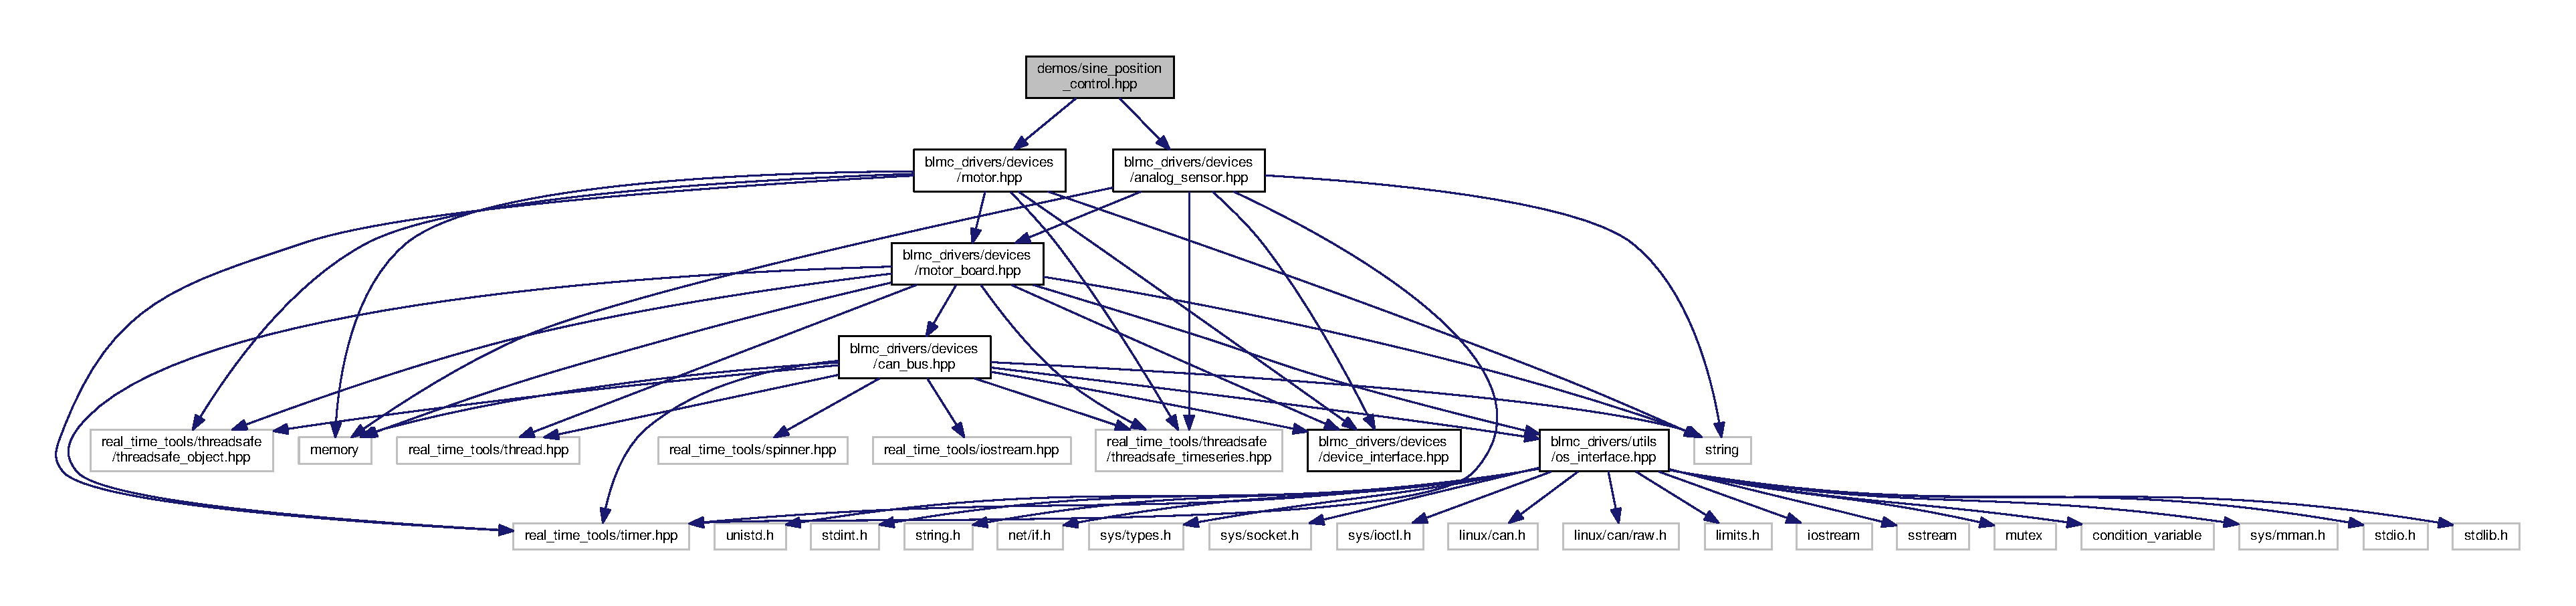
\includegraphics[width=350pt]{sine__position__control_8hpp__incl}
\end{center}
\end{figure}
This graph shows which files directly or indirectly include this file\+:
\nopagebreak
\begin{figure}[H]
\begin{center}
\leavevmode
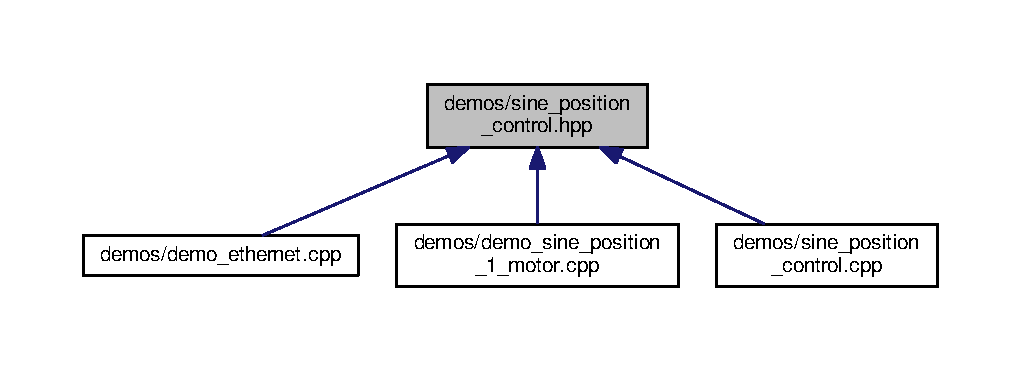
\includegraphics[width=350pt]{sine__position__control_8hpp__dep__incl}
\end{center}
\end{figure}
\subsection*{Classes}
\begin{DoxyCompactItemize}
\item 
class \hyperlink{classblmc__drivers_1_1SinePositionControl}{blmc\+\_\+drivers\+::\+Sine\+Position\+Control}
\begin{DoxyCompactList}\small\item\em This is a basic PD controller to be used in the demos of this package. \end{DoxyCompactList}\end{DoxyCompactItemize}
\subsection*{Namespaces}
\begin{DoxyCompactItemize}
\item 
 \hyperlink{namespaceblmc__drivers}{blmc\+\_\+drivers}
\begin{DoxyCompactList}\small\item\em This namespace is the standard namespace of the package. \end{DoxyCompactList}\end{DoxyCompactItemize}


\subsection{Detailed Description}
\begin{DoxyCopyright}{Copyright}
Copyright (c) 2018-\/2020, New York University and Max Planck Gesellschaft, License B\+S\+D-\/3-\/\+Clause 
\end{DoxyCopyright}

\hypertarget{sine__torque__control_8cpp}{}\section{demos/sine\+\_\+torque\+\_\+control.cpp File Reference}
\label{sine__torque__control_8cpp}\index{demos/sine\+\_\+torque\+\_\+control.\+cpp@{demos/sine\+\_\+torque\+\_\+control.\+cpp}}
{\ttfamily \#include $<$fstream$>$}\\*
{\ttfamily \#include \char`\"{}real\+\_\+time\+\_\+tools/timer.\+hpp\char`\"{}}\\*
{\ttfamily \#include \char`\"{}real\+\_\+time\+\_\+tools/spinner.\+hpp\char`\"{}}\\*
{\ttfamily \#include \char`\"{}sine\+\_\+torque\+\_\+control.\+hpp\char`\"{}}\\*
Include dependency graph for sine\+\_\+torque\+\_\+control.\+cpp\+:
\nopagebreak
\begin{figure}[H]
\begin{center}
\leavevmode
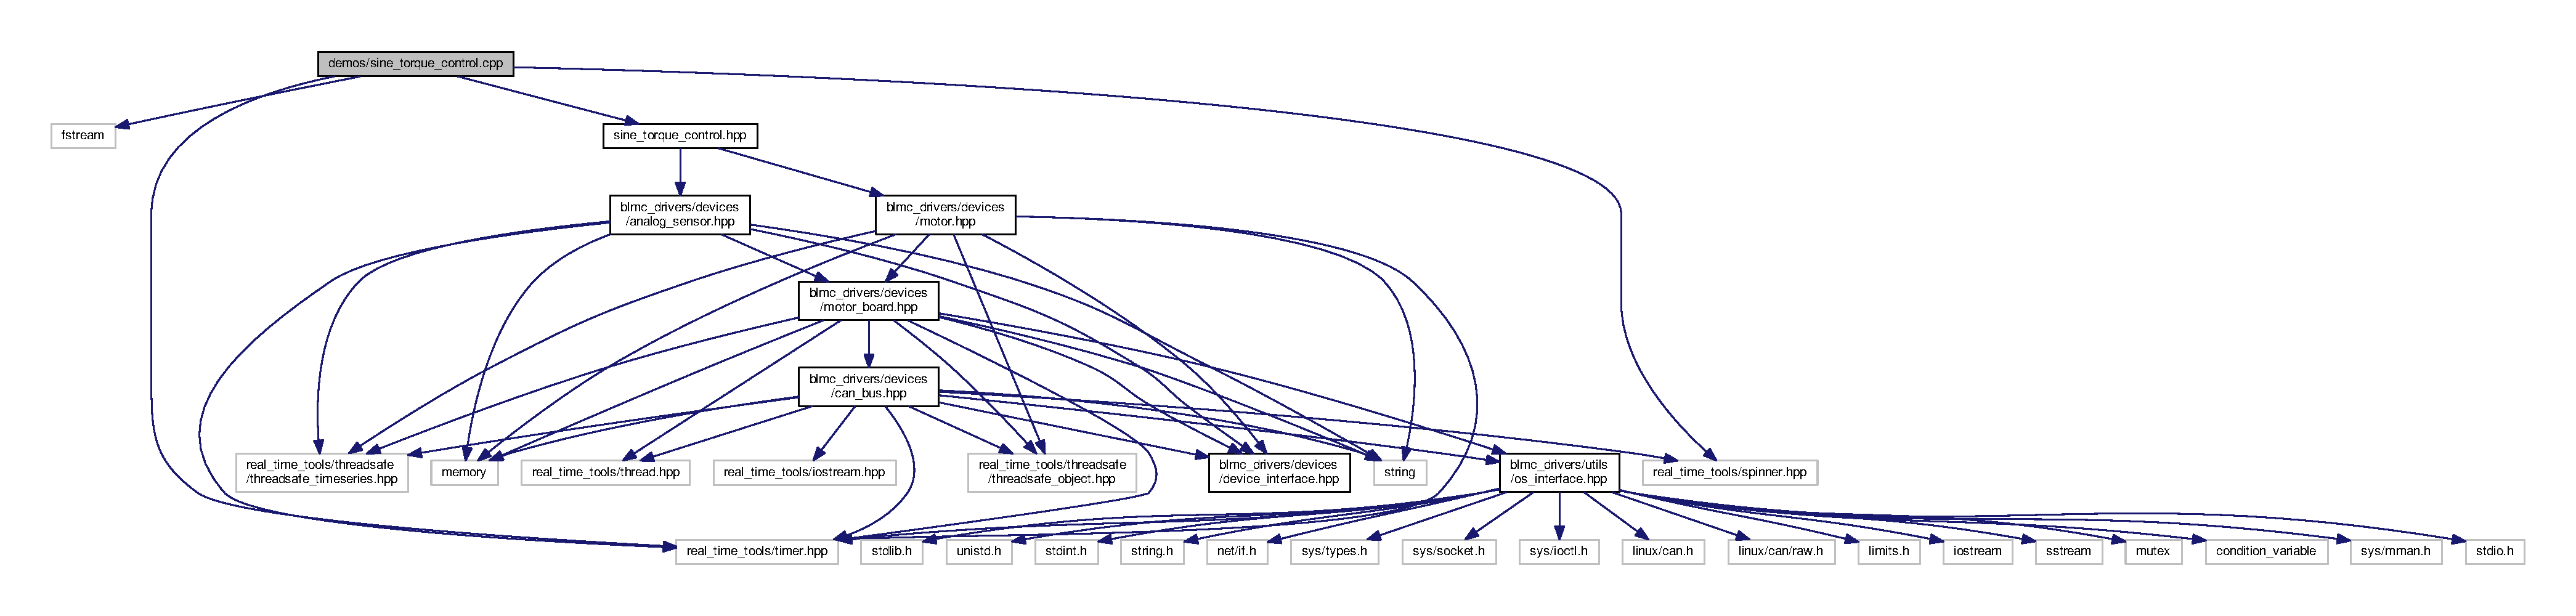
\includegraphics[width=350pt]{sine__torque__control_8cpp__incl}
\end{center}
\end{figure}
\subsection*{Namespaces}
\begin{DoxyCompactItemize}
\item 
 \hyperlink{namespaceblmc__drivers}{blmc\+\_\+drivers}
\begin{DoxyCompactList}\small\item\em This namespace is the standard namespace of the package. \end{DoxyCompactList}\end{DoxyCompactItemize}


\subsection{Detailed Description}
\begin{DoxyCopyright}{Copyright}
Copyright (c) 2018-\/2020, New York University and Max Planck Gesellschaft, License B\+S\+D-\/3-\/\+Clause 
\end{DoxyCopyright}

\hypertarget{sine__torque__control_8hpp}{}\section{demos/sine\+\_\+torque\+\_\+control.hpp File Reference}
\label{sine__torque__control_8hpp}\index{demos/sine\+\_\+torque\+\_\+control.\+hpp@{demos/sine\+\_\+torque\+\_\+control.\+hpp}}
{\ttfamily \#include \char`\"{}blmc\+\_\+drivers/devices/motor.\+hpp\char`\"{}}\\*
{\ttfamily \#include \char`\"{}blmc\+\_\+drivers/devices/analog\+\_\+sensor.\+hpp\char`\"{}}\\*
Include dependency graph for sine\+\_\+torque\+\_\+control.\+hpp\+:
\nopagebreak
\begin{figure}[H]
\begin{center}
\leavevmode
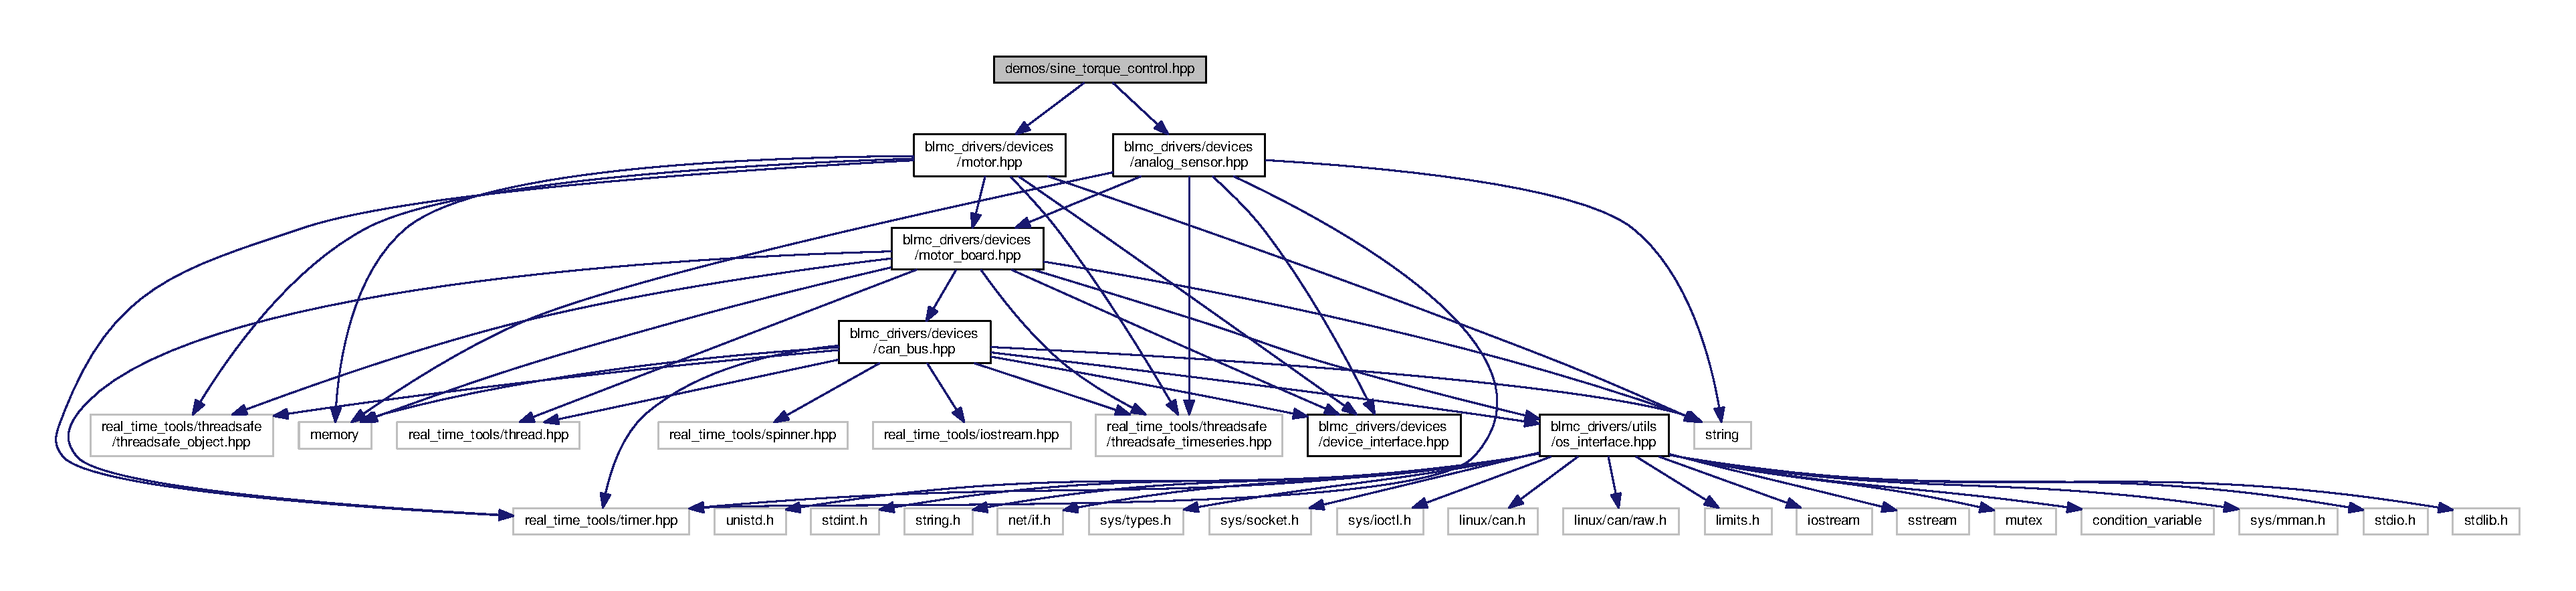
\includegraphics[width=350pt]{sine__torque__control_8hpp__incl}
\end{center}
\end{figure}
This graph shows which files directly or indirectly include this file\+:
\nopagebreak
\begin{figure}[H]
\begin{center}
\leavevmode
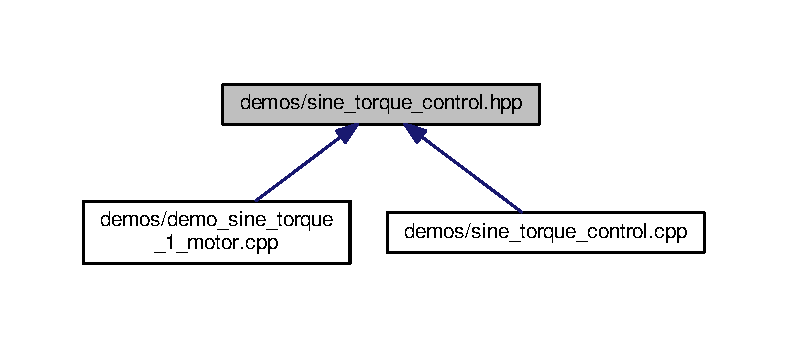
\includegraphics[width=350pt]{sine__torque__control_8hpp__dep__incl}
\end{center}
\end{figure}
\subsection*{Classes}
\begin{DoxyCompactItemize}
\item 
class \hyperlink{classblmc__drivers_1_1SineTorqueControl}{blmc\+\_\+drivers\+::\+Sine\+Torque\+Control}
\begin{DoxyCompactList}\small\item\em This is a basic PD controller to be used in the demos of this package. \end{DoxyCompactList}\end{DoxyCompactItemize}
\subsection*{Namespaces}
\begin{DoxyCompactItemize}
\item 
 \hyperlink{namespaceblmc__drivers}{blmc\+\_\+drivers}
\begin{DoxyCompactList}\small\item\em This namespace is the standard namespace of the package. \end{DoxyCompactList}\end{DoxyCompactItemize}


\subsection{Detailed Description}
\begin{DoxyCopyright}{Copyright}
Copyright (c) 2018-\/2020, New York University and Max Planck Gesellschaft, License B\+S\+D-\/3-\/\+Clause 
\end{DoxyCopyright}

\hypertarget{analog__sensor_8hpp}{}\section{include/blmc\+\_\+drivers/devices/analog\+\_\+sensor.hpp File Reference}
\label{analog__sensor_8hpp}\index{include/blmc\+\_\+drivers/devices/analog\+\_\+sensor.\+hpp@{include/blmc\+\_\+drivers/devices/analog\+\_\+sensor.\+hpp}}
{\ttfamily \#include $<$memory$>$}\\*
{\ttfamily \#include $<$string$>$}\\*
{\ttfamily \#include \char`\"{}real\+\_\+time\+\_\+tools/timer.\+hpp\char`\"{}}\\*
{\ttfamily \#include \char`\"{}real\+\_\+time\+\_\+tools/threadsafe/threadsafe\+\_\+timeseries.\+hpp\char`\"{}}\\*
{\ttfamily \#include \char`\"{}blmc\+\_\+drivers/devices/device\+\_\+interface.\+hpp\char`\"{}}\\*
{\ttfamily \#include \char`\"{}blmc\+\_\+drivers/devices/motor\+\_\+board.\+hpp\char`\"{}}\\*
Include dependency graph for analog\+\_\+sensor.\+hpp\+:
\nopagebreak
\begin{figure}[H]
\begin{center}
\leavevmode
\includegraphics[width=350pt]{analog__sensor_8hpp__incl}
\end{center}
\end{figure}
This graph shows which files directly or indirectly include this file\+:
\nopagebreak
\begin{figure}[H]
\begin{center}
\leavevmode
\includegraphics[width=350pt]{analog__sensor_8hpp__dep__incl}
\end{center}
\end{figure}
\subsection*{Classes}
\begin{DoxyCompactItemize}
\item 
class \hyperlink{classblmc__drivers_1_1AnalogSensorInterface}{blmc\+\_\+drivers\+::\+Analog\+Sensor\+Interface}
\begin{DoxyCompactList}\small\item\em \hyperlink{classblmc__drivers_1_1AnalogSensorInterface}{Analog\+Sensor\+Interface} class is a simple abstract interface for using blmc analog measurements. \end{DoxyCompactList}\item 
class \hyperlink{classblmc__drivers_1_1AnalogSensor}{blmc\+\_\+drivers\+::\+Analog\+Sensor}
\begin{DoxyCompactList}\small\item\em \hyperlink{classblmc__drivers_1_1AnalogSensor}{Analog\+Sensor} class is the implementation of the above interface. \end{DoxyCompactList}\end{DoxyCompactItemize}
\subsection*{Namespaces}
\begin{DoxyCompactItemize}
\item 
 \hyperlink{namespaceblmc__drivers}{blmc\+\_\+drivers}
\begin{DoxyCompactList}\small\item\em This namespace is the standard namespace of the package. \end{DoxyCompactList}\end{DoxyCompactItemize}


\subsection{Detailed Description}
\begin{DoxyRefDesc}{License}
\item[\hyperlink{license__license000001}{License}]License B\+S\+D-\/3-\/\+Clause \end{DoxyRefDesc}
\begin{DoxyCopyright}{Copyright}
Copyright (c) 2019, New York University and Max Planck Gesellshaft. 
\end{DoxyCopyright}
\begin{DoxyDate}{Date}
2019-\/07-\/11 
\end{DoxyDate}

\hypertarget{can__bus_8hpp}{}\section{include/blmc\+\_\+drivers/devices/can\+\_\+bus.hpp File Reference}
\label{can__bus_8hpp}\index{include/blmc\+\_\+drivers/devices/can\+\_\+bus.\+hpp@{include/blmc\+\_\+drivers/devices/can\+\_\+bus.\+hpp}}
{\ttfamily \#include $<$memory$>$}\\*
{\ttfamily \#include $<$string$>$}\\*
{\ttfamily \#include \char`\"{}real\+\_\+time\+\_\+tools/timer.\+hpp\char`\"{}}\\*
{\ttfamily \#include \char`\"{}real\+\_\+time\+\_\+tools/thread.\+hpp\char`\"{}}\\*
{\ttfamily \#include \char`\"{}real\+\_\+time\+\_\+tools/iostream.\+hpp\char`\"{}}\\*
{\ttfamily \#include \char`\"{}real\+\_\+time\+\_\+tools/spinner.\+hpp\char`\"{}}\\*
{\ttfamily \#include \char`\"{}real\+\_\+time\+\_\+tools/threadsafe/threadsafe\+\_\+object.\+hpp\char`\"{}}\\*
{\ttfamily \#include \char`\"{}real\+\_\+time\+\_\+tools/threadsafe/threadsafe\+\_\+timeseries.\+hpp\char`\"{}}\\*
{\ttfamily \#include \char`\"{}blmc\+\_\+drivers/utils/os\+\_\+interface.\+hpp\char`\"{}}\\*
{\ttfamily \#include \char`\"{}blmc\+\_\+drivers/devices/device\+\_\+interface.\+hpp\char`\"{}}\\*
Include dependency graph for can\+\_\+bus.\+hpp\+:
\nopagebreak
\begin{figure}[H]
\begin{center}
\leavevmode
\includegraphics[width=350pt]{can__bus_8hpp__incl}
\end{center}
\end{figure}
This graph shows which files directly or indirectly include this file\+:
\nopagebreak
\begin{figure}[H]
\begin{center}
\leavevmode
\includegraphics[width=350pt]{can__bus_8hpp__dep__incl}
\end{center}
\end{figure}
\subsection*{Classes}
\begin{DoxyCompactItemize}
\item 
class \hyperlink{classblmc__drivers_1_1CanBusFrame}{blmc\+\_\+drivers\+::\+Can\+Bus\+Frame}
\begin{DoxyCompactList}\small\item\em \hyperlink{classblmc__drivers_1_1CanBusFrame}{Can\+Bus\+Frame} is a class that contains a fixed sized amount of data to be send or received via the can bus. \end{DoxyCompactList}\item 
class \hyperlink{classblmc__drivers_1_1CanBusConnection}{blmc\+\_\+drivers\+::\+Can\+Bus\+Connection}
\begin{DoxyCompactList}\small\item\em \hyperlink{classblmc__drivers_1_1CanBusConnection}{Can\+Bus\+Connection} is a data structure that contains the hardware details for the connection between to can cards. \end{DoxyCompactList}\item 
class \hyperlink{classblmc__drivers_1_1CanBusInterface}{blmc\+\_\+drivers\+::\+Can\+Bus\+Interface}
\begin{DoxyCompactList}\small\item\em \hyperlink{classblmc__drivers_1_1CanBusInterface}{Can\+Bus\+Interface} is an abstract class that defines an A\+PI for the communication via Can bus. \end{DoxyCompactList}\item 
class \hyperlink{classblmc__drivers_1_1CanBus}{blmc\+\_\+drivers\+::\+Can\+Bus}
\begin{DoxyCompactList}\small\item\em \hyperlink{classblmc__drivers_1_1CanBus}{Can\+Bus} is the implementation of the \hyperlink{classblmc__drivers_1_1CanBusInterface}{Can\+Bus\+Interface}. \end{DoxyCompactList}\end{DoxyCompactItemize}
\subsection*{Namespaces}
\begin{DoxyCompactItemize}
\item 
 \hyperlink{namespaceblmc__drivers}{blmc\+\_\+drivers}
\begin{DoxyCompactList}\small\item\em This namespace is the standard namespace of the package. \end{DoxyCompactList}\end{DoxyCompactItemize}


\subsection{Detailed Description}
\begin{DoxyRefDesc}{License}
\item[\hyperlink{license__license000002}{License}]License B\+S\+D-\/3-\/\+Clause \end{DoxyRefDesc}
\begin{DoxyCopyright}{Copyright}
Copyright (c) 2019, New York University and Max Planck Gesellshaft. 
\end{DoxyCopyright}
\begin{DoxyDate}{Date}
2019-\/07-\/11 
\end{DoxyDate}

\hypertarget{device__interface_8hpp}{}\section{include/blmc\+\_\+drivers/devices/device\+\_\+interface.hpp File Reference}
\label{device__interface_8hpp}\index{include/blmc\+\_\+drivers/devices/device\+\_\+interface.\+hpp@{include/blmc\+\_\+drivers/devices/device\+\_\+interface.\+hpp}}
This graph shows which files directly or indirectly include this file\+:
\nopagebreak
\begin{figure}[H]
\begin{center}
\leavevmode
\includegraphics[width=350pt]{device__interface_8hpp__dep__incl}
\end{center}
\end{figure}
\subsection*{Classes}
\begin{DoxyCompactItemize}
\item 
class \hyperlink{classblmc__drivers_1_1DeviceInterface}{blmc\+\_\+drivers\+::\+Device\+Interface}
\begin{DoxyCompactList}\small\item\em this class exists purely for logical reasons, it does not in itself implement anything. \end{DoxyCompactList}\end{DoxyCompactItemize}
\subsection*{Namespaces}
\begin{DoxyCompactItemize}
\item 
 \hyperlink{namespaceblmc__drivers}{blmc\+\_\+drivers}
\begin{DoxyCompactList}\small\item\em This namespace is the standard namespace of the package. \end{DoxyCompactList}\end{DoxyCompactItemize}


\subsection{Detailed Description}
\begin{DoxyRefDesc}{License}
\item[\hyperlink{license__license000003}{License}]License B\+S\+D-\/3-\/\+Clause \end{DoxyRefDesc}
\begin{DoxyCopyright}{Copyright}
Copyright (c) 2019, New York University and Max Planck Gesellshaft. 
\end{DoxyCopyright}
\begin{DoxyDate}{Date}
2019-\/07-\/11 
\end{DoxyDate}

\hypertarget{leg_8hpp}{}\section{include/blmc\+\_\+drivers/devices/leg.hpp File Reference}
\label{leg_8hpp}\index{include/blmc\+\_\+drivers/devices/leg.\+hpp@{include/blmc\+\_\+drivers/devices/leg.\+hpp}}
{\ttfamily \#include $<$memory$>$}\\*
{\ttfamily \#include $<$string$>$}\\*
{\ttfamily \#include $<$map$>$}\\*
{\ttfamily \#include $<$real\+\_\+time\+\_\+tools/threadsafe/threadsafe\+\_\+timeseries.\+hpp$>$}\\*
{\ttfamily \#include $<$blmc\+\_\+drivers/devices/motor.\+hpp$>$}\\*
{\ttfamily \#include $<$blmc\+\_\+drivers/devices/device\+\_\+interface.\+hpp$>$}\\*
Include dependency graph for leg.\+hpp\+:
\nopagebreak
\begin{figure}[H]
\begin{center}
\leavevmode
\includegraphics[width=350pt]{leg_8hpp__incl}
\end{center}
\end{figure}
This graph shows which files directly or indirectly include this file\+:
\nopagebreak
\begin{figure}[H]
\begin{center}
\leavevmode
\includegraphics[width=190pt]{leg_8hpp__dep__incl}
\end{center}
\end{figure}
\subsection*{Classes}
\begin{DoxyCompactItemize}
\item 
class \hyperlink{classblmc__drivers_1_1LegInterface}{blmc\+\_\+drivers\+::\+Leg\+Interface}
\begin{DoxyCompactList}\small\item\em This class defines an interface to control a leg. \end{DoxyCompactList}\item 
class \hyperlink{classblmc__drivers_1_1Leg}{blmc\+\_\+drivers\+::\+Leg}
\begin{DoxyCompactList}\small\item\em The leg class is the implementation of the \hyperlink{classblmc__drivers_1_1LegInterface}{Leg\+Interface}. \end{DoxyCompactList}\end{DoxyCompactItemize}
\subsection*{Namespaces}
\begin{DoxyCompactItemize}
\item 
 \hyperlink{namespaceblmc__drivers}{blmc\+\_\+drivers}
\begin{DoxyCompactList}\small\item\em This namespace is the standard namespace of the package. \end{DoxyCompactList}\end{DoxyCompactItemize}


\subsection{Detailed Description}
\begin{DoxyRefDesc}{License}
\item[\hyperlink{license__license000004}{License}]License B\+S\+D-\/3-\/\+Clause \end{DoxyRefDesc}
\begin{DoxyCopyright}{Copyright}
Copyright (c) 2019, New York University and Max Planck Gesellshaft. 
\end{DoxyCopyright}
\begin{DoxyDate}{Date}
2019-\/07-\/11 
\end{DoxyDate}

\hypertarget{motor_8hpp}{}\section{include/blmc\+\_\+drivers/devices/motor.hpp File Reference}
\label{motor_8hpp}\index{include/blmc\+\_\+drivers/devices/motor.\+hpp@{include/blmc\+\_\+drivers/devices/motor.\+hpp}}
{\ttfamily \#include $<$memory$>$}\\*
{\ttfamily \#include $<$string$>$}\\*
{\ttfamily \#include \char`\"{}real\+\_\+time\+\_\+tools/timer.\+hpp\char`\"{}}\\*
{\ttfamily \#include \char`\"{}real\+\_\+time\+\_\+tools/threadsafe/threadsafe\+\_\+object.\+hpp\char`\"{}}\\*
{\ttfamily \#include \char`\"{}real\+\_\+time\+\_\+tools/threadsafe/threadsafe\+\_\+timeseries.\+hpp\char`\"{}}\\*
{\ttfamily \#include \char`\"{}blmc\+\_\+drivers/devices/motor\+\_\+board.\+hpp\char`\"{}}\\*
{\ttfamily \#include \char`\"{}blmc\+\_\+drivers/devices/device\+\_\+interface.\+hpp\char`\"{}}\\*
Include dependency graph for motor.\+hpp\+:
\nopagebreak
\begin{figure}[H]
\begin{center}
\leavevmode
\includegraphics[width=350pt]{motor_8hpp__incl}
\end{center}
\end{figure}
This graph shows which files directly or indirectly include this file\+:
\nopagebreak
\begin{figure}[H]
\begin{center}
\leavevmode
\includegraphics[width=350pt]{motor_8hpp__dep__incl}
\end{center}
\end{figure}
\subsection*{Classes}
\begin{DoxyCompactItemize}
\item 
class \hyperlink{classblmc__drivers_1_1MotorInterface}{blmc\+\_\+drivers\+::\+Motor\+Interface}
\begin{DoxyCompactList}\small\item\em This class declares an interface to the motor. \end{DoxyCompactList}\item 
class \hyperlink{classblmc__drivers_1_1Motor}{blmc\+\_\+drivers\+::\+Motor}
\begin{DoxyCompactList}\small\item\em This class implements the \hyperlink{classblmc__drivers_1_1MotorInterface}{Motor\+Interface}. \end{DoxyCompactList}\item 
class \hyperlink{classblmc__drivers_1_1SafeMotor}{blmc\+\_\+drivers\+::\+Safe\+Motor}
\begin{DoxyCompactList}\small\item\em This class is a safe implementation of the \hyperlink{classblmc__drivers_1_1Motor}{Motor} class. \end{DoxyCompactList}\end{DoxyCompactItemize}
\subsection*{Namespaces}
\begin{DoxyCompactItemize}
\item 
 \hyperlink{namespaceblmc__drivers}{blmc\+\_\+drivers}
\begin{DoxyCompactList}\small\item\em This namespace is the standard namespace of the package. \end{DoxyCompactList}\end{DoxyCompactItemize}


\subsection{Detailed Description}
\begin{DoxyRefDesc}{License}
\item[\hyperlink{license__license000005}{License}]License B\+S\+D-\/3-\/\+Clause \end{DoxyRefDesc}
\begin{DoxyCopyright}{Copyright}
Copyright (c) 2019-\/2020, New York University and Max Planck Gesellshaft. 
\end{DoxyCopyright}
\begin{DoxyDate}{Date}
2019-\/07-\/11 
\end{DoxyDate}

\hypertarget{motor__board_8hpp}{}\section{include/blmc\+\_\+drivers/devices/motor\+\_\+board.hpp File Reference}
\label{motor__board_8hpp}\index{include/blmc\+\_\+drivers/devices/motor\+\_\+board.\+hpp@{include/blmc\+\_\+drivers/devices/motor\+\_\+board.\+hpp}}
{\ttfamily \#include $<$memory$>$}\\*
{\ttfamily \#include $<$string$>$}\\*
{\ttfamily \#include \char`\"{}real\+\_\+time\+\_\+tools/timer.\+hpp\char`\"{}}\\*
{\ttfamily \#include \char`\"{}real\+\_\+time\+\_\+tools/thread.\+hpp\char`\"{}}\\*
{\ttfamily \#include \char`\"{}blmc\+\_\+drivers/utils/os\+\_\+interface.\+hpp\char`\"{}}\\*
{\ttfamily \#include \char`\"{}real\+\_\+time\+\_\+tools/threadsafe/threadsafe\+\_\+object.\+hpp\char`\"{}}\\*
{\ttfamily \#include \char`\"{}real\+\_\+time\+\_\+tools/threadsafe/threadsafe\+\_\+timeseries.\+hpp\char`\"{}}\\*
{\ttfamily \#include \char`\"{}blmc\+\_\+drivers/devices/can\+\_\+bus.\+hpp\char`\"{}}\\*
{\ttfamily \#include \char`\"{}blmc\+\_\+drivers/devices/device\+\_\+interface.\+hpp\char`\"{}}\\*
Include dependency graph for motor\+\_\+board.\+hpp\+:
\nopagebreak
\begin{figure}[H]
\begin{center}
\leavevmode
\includegraphics[width=350pt]{motor__board_8hpp__incl}
\end{center}
\end{figure}
This graph shows which files directly or indirectly include this file\+:
\nopagebreak
\begin{figure}[H]
\begin{center}
\leavevmode
\includegraphics[width=350pt]{motor__board_8hpp__dep__incl}
\end{center}
\end{figure}
\subsection*{Classes}
\begin{DoxyCompactItemize}
\item 
class \hyperlink{classblmc__drivers_1_1MotorBoardCommand}{blmc\+\_\+drivers\+::\+Motor\+Board\+Command}
\begin{DoxyCompactList}\small\item\em This \hyperlink{classblmc__drivers_1_1MotorBoardCommand}{Motor\+Board\+Command} class is a data structurs that defines a command. \end{DoxyCompactList}\item 
class \hyperlink{classblmc__drivers_1_1MotorBoardStatus}{blmc\+\_\+drivers\+::\+Motor\+Board\+Status}
\begin{DoxyCompactList}\small\item\em This class represent a 8 bits message that describe the state (enable/disabled) of the card and the two motors. \end{DoxyCompactList}\item 
class \hyperlink{classblmc__drivers_1_1MotorBoardInterface}{blmc\+\_\+drivers\+::\+Motor\+Board\+Interface}
\begin{DoxyCompactList}\small\item\em \hyperlink{classblmc__drivers_1_1MotorBoardInterface}{Motor\+Board\+Interface} declares an A\+PI to inacte with a Motor\+Board. \end{DoxyCompactList}\item 
class \hyperlink{classblmc__drivers_1_1CanBusMotorBoard}{blmc\+\_\+drivers\+::\+Can\+Bus\+Motor\+Board}
\begin{DoxyCompactList}\small\item\em This class \hyperlink{classblmc__drivers_1_1CanBusMotorBoard}{Can\+Bus\+Motor\+Board} implements a \hyperlink{classblmc__drivers_1_1MotorBoardInterface}{Motor\+Board\+Interface} specific to C\+AN networks. \end{DoxyCompactList}\end{DoxyCompactItemize}
\subsection*{Namespaces}
\begin{DoxyCompactItemize}
\item 
 \hyperlink{namespaceblmc__drivers}{blmc\+\_\+drivers}
\begin{DoxyCompactList}\small\item\em This namespace is the standard namespace of the package. \end{DoxyCompactList}\end{DoxyCompactItemize}
\subsection*{Functions}
\begin{DoxyCompactItemize}
\item 
{\footnotesize template$<$typename Type $>$ }\\std\+::vector$<$ std\+::shared\+\_\+ptr$<$ Type $>$ $>$ \hyperlink{namespaceblmc__drivers_add73ea2a43509013ad00665753f175e1}{blmc\+\_\+drivers\+::create\+\_\+vector\+\_\+of\+\_\+pointers} (const size\+\_\+t \&size, const size\+\_\+t \&length)
\begin{DoxyCompactList}\small\item\em Create a vector of pointers. \end{DoxyCompactList}\end{DoxyCompactItemize}


\subsection{Detailed Description}
\begin{DoxyRefDesc}{License}
\item[\hyperlink{license__license000006}{License}]License B\+S\+D-\/3-\/\+Clause \end{DoxyRefDesc}
\begin{DoxyCopyright}{Copyright}
Copyright (c) 2019, New York University and Max Planck Gesellshaft. 
\end{DoxyCopyright}
\begin{DoxyDate}{Date}
2019-\/07-\/11 
\end{DoxyDate}

\hypertarget{spi__bus_8hpp}{}\section{include/blmc\+\_\+drivers/devices/spi\+\_\+bus.hpp File Reference}
\label{spi__bus_8hpp}\index{include/blmc\+\_\+drivers/devices/spi\+\_\+bus.\+hpp@{include/blmc\+\_\+drivers/devices/spi\+\_\+bus.\+hpp}}


Interface for the main board designed by Thomas Floyols \href{https://github.com/open-dynamic-robot-initiative/master-board}{\tt https\+://github.\+com/open-\/dynamic-\/robot-\/initiative/master-\/board}.  


{\ttfamily \#include \char`\"{}master\+\_\+board\+\_\+sdk/master\+\_\+board\+\_\+interface.\+h\char`\"{}}\\*
{\ttfamily \#include \char`\"{}blmc\+\_\+drivers/devices/motor.\+hpp\char`\"{}}\\*
{\ttfamily \#include \char`\"{}real\+\_\+time\+\_\+tools/thread.\+hpp\char`\"{}}\\*
{\ttfamily \#include \char`\"{}real\+\_\+time\+\_\+tools/threadsafe/threadsafe\+\_\+timeseries.\+hpp\char`\"{}}\\*
{\ttfamily \#include \char`\"{}blmc\+\_\+drivers/devices/motor\+\_\+board.\+hpp\char`\"{}}\\*
Include dependency graph for spi\+\_\+bus.\+hpp\+:
\nopagebreak
\begin{figure}[H]
\begin{center}
\leavevmode
\includegraphics[width=350pt]{spi__bus_8hpp__incl}
\end{center}
\end{figure}
This graph shows which files directly or indirectly include this file\+:
\nopagebreak
\begin{figure}[H]
\begin{center}
\leavevmode
\includegraphics[width=350pt]{spi__bus_8hpp__dep__incl}
\end{center}
\end{figure}
\subsection*{Classes}
\begin{DoxyCompactItemize}
\item 
class \hyperlink{classblmc__drivers_1_1SpiBus}{blmc\+\_\+drivers\+::\+Spi\+Bus}
\end{DoxyCompactItemize}
\subsection*{Namespaces}
\begin{DoxyCompactItemize}
\item 
 \hyperlink{namespaceblmc__drivers}{blmc\+\_\+drivers}
\begin{DoxyCompactList}\small\item\em This namespace is the standard namespace of the package. \end{DoxyCompactList}\end{DoxyCompactItemize}


\subsection{Detailed Description}
Interface for the main board designed by Thomas Floyols \href{https://github.com/open-dynamic-robot-initiative/master-board}{\tt https\+://github.\+com/open-\/dynamic-\/robot-\/initiative/master-\/board}. 

\begin{DoxyAuthor}{Author}
Maximilien Naveau (\href{mailto:maximilien.naveau@gmail.com}{\tt maximilien.\+naveau@gmail.\+com}) 
\end{DoxyAuthor}
\begin{DoxyVersion}{Version}
0.\+1 
\end{DoxyVersion}
\begin{DoxyDate}{Date}
2019-\/11-\/14
\end{DoxyDate}
\begin{DoxyCopyright}{Copyright}
Copyright (c) 2019-\/2020, New York University and Max Planck Gesellshaft. 
\end{DoxyCopyright}

\hypertarget{spi__motor__board_8hpp}{}\section{include/blmc\+\_\+drivers/devices/spi\+\_\+motor\+\_\+board.hpp File Reference}
\label{spi__motor__board_8hpp}\index{include/blmc\+\_\+drivers/devices/spi\+\_\+motor\+\_\+board.\+hpp@{include/blmc\+\_\+drivers/devices/spi\+\_\+motor\+\_\+board.\+hpp}}


Interface for the master board designed by Thomas Floyols \href{https://github.com/open-dynamic-robot-initiative/master-board}{\tt https\+://github.\+com/open-\/dynamic-\/robot-\/initiative/master-\/board}.  


{\ttfamily \#include \char`\"{}blmc\+\_\+drivers/devices/spi\+\_\+bus.\+hpp\char`\"{}}\\*
{\ttfamily \#include \char`\"{}real\+\_\+time\+\_\+tools/thread.\+hpp\char`\"{}}\\*
{\ttfamily \#include \char`\"{}real\+\_\+time\+\_\+tools/threadsafe/threadsafe\+\_\+timeseries.\+hpp\char`\"{}}\\*
{\ttfamily \#include \char`\"{}blmc\+\_\+drivers/devices/motor\+\_\+board.\+hpp\char`\"{}}\\*
Include dependency graph for spi\+\_\+motor\+\_\+board.\+hpp\+:
\nopagebreak
\begin{figure}[H]
\begin{center}
\leavevmode
\includegraphics[width=350pt]{spi__motor__board_8hpp__incl}
\end{center}
\end{figure}
This graph shows which files directly or indirectly include this file\+:
\nopagebreak
\begin{figure}[H]
\begin{center}
\leavevmode
\includegraphics[width=350pt]{spi__motor__board_8hpp__dep__incl}
\end{center}
\end{figure}
\subsection*{Classes}
\begin{DoxyCompactItemize}
\item 
class \hyperlink{classblmc__drivers_1_1SpiMotorBoard}{blmc\+\_\+drivers\+::\+Spi\+Motor\+Board}
\end{DoxyCompactItemize}
\subsection*{Namespaces}
\begin{DoxyCompactItemize}
\item 
 \hyperlink{namespaceblmc__drivers}{blmc\+\_\+drivers}
\begin{DoxyCompactList}\small\item\em This namespace is the standard namespace of the package. \end{DoxyCompactList}\end{DoxyCompactItemize}


\subsection{Detailed Description}
Interface for the master board designed by Thomas Floyols \href{https://github.com/open-dynamic-robot-initiative/master-board}{\tt https\+://github.\+com/open-\/dynamic-\/robot-\/initiative/master-\/board}. 

\begin{DoxyAuthor}{Author}
Maximilien Naveau (\href{mailto:maximilien.naveau@gmail.com}{\tt maximilien.\+naveau@gmail.\+com}) 
\end{DoxyAuthor}
\begin{DoxyVersion}{Version}
0.\+1 
\end{DoxyVersion}
\begin{DoxyDate}{Date}
2019-\/11-\/14
\end{DoxyDate}
\begin{DoxyCopyright}{Copyright}
Copyright (c) 2019-\/2020, New York University and Max Planck Gesellshaft. 
\end{DoxyCopyright}

\hypertarget{serial__reader_8hpp}{}\section{include/blmc\+\_\+drivers/serial\+\_\+reader.hpp File Reference}
\label{serial__reader_8hpp}\index{include/blmc\+\_\+drivers/serial\+\_\+reader.\+hpp@{include/blmc\+\_\+drivers/serial\+\_\+reader.\+hpp}}


Wrapper for reading new-\/line terminated list of values from serial port.  


{\ttfamily \#include $<$cstdlib$>$}\\*
{\ttfamily \#include $<$iostream$>$}\\*
{\ttfamily \#include $<$mutex$>$}\\*
{\ttfamily \#include $<$unistd.\+h$>$}\\*
{\ttfamily \#include $<$vector$>$}\\*
{\ttfamily \#include \char`\"{}real\+\_\+time\+\_\+tools/thread.\+hpp\char`\"{}}\\*
Include dependency graph for serial\+\_\+reader.\+hpp\+:
\nopagebreak
\begin{figure}[H]
\begin{center}
\leavevmode
\includegraphics[width=350pt]{serial__reader_8hpp__incl}
\end{center}
\end{figure}
This graph shows which files directly or indirectly include this file\+:
\nopagebreak
\begin{figure}[H]
\begin{center}
\leavevmode
\includegraphics[width=187pt]{serial__reader_8hpp__dep__incl}
\end{center}
\end{figure}
\subsection*{Classes}
\begin{DoxyCompactItemize}
\item 
class \hyperlink{classblmc__drivers_1_1SerialReader}{blmc\+\_\+drivers\+::\+Serial\+Reader}
\end{DoxyCompactItemize}
\subsection*{Namespaces}
\begin{DoxyCompactItemize}
\item 
 \hyperlink{namespaceblmc__drivers}{blmc\+\_\+drivers}
\begin{DoxyCompactList}\small\item\em This namespace is the standard namespace of the package. \end{DoxyCompactList}\end{DoxyCompactItemize}


\subsection{Detailed Description}
Wrapper for reading new-\/line terminated list of values from serial port. 

\begin{DoxyAuthor}{Author}
Julian Viereck 
\end{DoxyAuthor}
\begin{DoxyDate}{Date}
2020 
\end{DoxyDate}
\begin{DoxyCopyright}{Copyright}
Copyright (c) 2020, New York University and Max Planck Gesellschaft. 
\end{DoxyCopyright}

\hypertarget{os__interface_8hpp}{}\section{include/blmc\+\_\+drivers/utils/os\+\_\+interface.hpp File Reference}
\label{os__interface_8hpp}\index{include/blmc\+\_\+drivers/utils/os\+\_\+interface.\+hpp@{include/blmc\+\_\+drivers/utils/os\+\_\+interface.\+hpp}}
{\ttfamily \#include $<$stdio.\+h$>$}\\*
{\ttfamily \#include $<$stdlib.\+h$>$}\\*
{\ttfamily \#include $<$unistd.\+h$>$}\\*
{\ttfamily \#include $<$stdint.\+h$>$}\\*
{\ttfamily \#include $<$string.\+h$>$}\\*
{\ttfamily \#include $<$net/if.\+h$>$}\\*
{\ttfamily \#include $<$sys/types.\+h$>$}\\*
{\ttfamily \#include $<$sys/socket.\+h$>$}\\*
{\ttfamily \#include $<$sys/ioctl.\+h$>$}\\*
{\ttfamily \#include $<$linux/can.\+h$>$}\\*
{\ttfamily \#include $<$linux/can/raw.\+h$>$}\\*
{\ttfamily \#include $<$limits.\+h$>$}\\*
{\ttfamily \#include $<$real\+\_\+time\+\_\+tools/timer.\+hpp$>$}\\*
{\ttfamily \#include $<$iostream$>$}\\*
{\ttfamily \#include $<$sstream$>$}\\*
{\ttfamily \#include $<$mutex$>$}\\*
{\ttfamily \#include $<$condition\+\_\+variable$>$}\\*
{\ttfamily \#include $<$sys/mman.\+h$>$}\\*
Include dependency graph for os\+\_\+interface.\+hpp\+:
\nopagebreak
\begin{figure}[H]
\begin{center}
\leavevmode
\includegraphics[width=350pt]{os__interface_8hpp__incl}
\end{center}
\end{figure}
This graph shows which files directly or indirectly include this file\+:
\nopagebreak
\begin{figure}[H]
\begin{center}
\leavevmode
\includegraphics[width=350pt]{os__interface_8hpp__dep__incl}
\end{center}
\end{figure}
\subsection*{Namespaces}
\begin{DoxyCompactItemize}
\item 
 \hyperlink{namespaceosi}{osi}
\begin{DoxyCompactList}\small\item\em Common include. \end{DoxyCompactList}\end{DoxyCompactItemize}
\subsection*{Macros}
\begin{DoxyCompactItemize}
\item 
\#define \hyperlink{os__interface_8hpp_a25df6b00e3fd8b8740896ecc5c337fdc}{rt\+\_\+fprintf}~fprintf\hypertarget{os__interface_8hpp_a25df6b00e3fd8b8740896ecc5c337fdc}{}\label{os__interface_8hpp_a25df6b00e3fd8b8740896ecc5c337fdc}

\begin{DoxyCompactList}\small\item\em Create a common type\+\_\+def to wrap xenomai and posix. \end{DoxyCompactList}\item 
\#define \hyperlink{os__interface_8hpp_a1acf1ce04ab7fe3a5972c0618adcbbac}{rt\+\_\+printf}~printf\hypertarget{os__interface_8hpp_a1acf1ce04ab7fe3a5972c0618adcbbac}{}\label{os__interface_8hpp_a1acf1ce04ab7fe3a5972c0618adcbbac}

\begin{DoxyCompactList}\small\item\em Create a common type\+\_\+def to wrap xenomai and posix. \end{DoxyCompactList}\item 
\#define \hyperlink{os__interface_8hpp_ac420926cbb955a79a41eba7cec1bc1c8}{rt\+\_\+dev\+\_\+socket}~socket\hypertarget{os__interface_8hpp_ac420926cbb955a79a41eba7cec1bc1c8}{}\label{os__interface_8hpp_ac420926cbb955a79a41eba7cec1bc1c8}

\begin{DoxyCompactList}\small\item\em Create a common type\+\_\+def to wrap xenomai and posix. \end{DoxyCompactList}\item 
\#define \hyperlink{os__interface_8hpp_a81e55d2bdf351cd53218a3085ba56955}{rt\+\_\+dev\+\_\+ioctl}~ioctl\hypertarget{os__interface_8hpp_a81e55d2bdf351cd53218a3085ba56955}{}\label{os__interface_8hpp_a81e55d2bdf351cd53218a3085ba56955}

\begin{DoxyCompactList}\small\item\em Create a common type\+\_\+def to wrap xenomai and posix. \end{DoxyCompactList}\item 
\#define \hyperlink{os__interface_8hpp_a7be59cefa5f5e5da067c04078f504aa6}{rt\+\_\+dev\+\_\+close}~close\hypertarget{os__interface_8hpp_a7be59cefa5f5e5da067c04078f504aa6}{}\label{os__interface_8hpp_a7be59cefa5f5e5da067c04078f504aa6}

\begin{DoxyCompactList}\small\item\em Create a common type\+\_\+def to wrap xenomai and posix. \end{DoxyCompactList}\item 
\#define \hyperlink{os__interface_8hpp_a80d28afb04b8db1e0192593ebcb4d07b}{rt\+\_\+dev\+\_\+setsockopt}~setsockopt\hypertarget{os__interface_8hpp_a80d28afb04b8db1e0192593ebcb4d07b}{}\label{os__interface_8hpp_a80d28afb04b8db1e0192593ebcb4d07b}

\begin{DoxyCompactList}\small\item\em Create a common type\+\_\+def to wrap xenomai and posix. \end{DoxyCompactList}\item 
\#define \hyperlink{os__interface_8hpp_a68219f584f63b92f4d23bd708140056d}{rt\+\_\+dev\+\_\+bind}~bind\hypertarget{os__interface_8hpp_a68219f584f63b92f4d23bd708140056d}{}\label{os__interface_8hpp_a68219f584f63b92f4d23bd708140056d}

\begin{DoxyCompactList}\small\item\em Create a common type\+\_\+def to wrap xenomai and posix. \end{DoxyCompactList}\item 
\#define \hyperlink{os__interface_8hpp_ab599460d70a4af2e3bcb07b395f13ad4}{rt\+\_\+dev\+\_\+recvmsg}~recvmsg\hypertarget{os__interface_8hpp_ab599460d70a4af2e3bcb07b395f13ad4}{}\label{os__interface_8hpp_ab599460d70a4af2e3bcb07b395f13ad4}

\begin{DoxyCompactList}\small\item\em Create a common type\+\_\+def to wrap xenomai and posix. \end{DoxyCompactList}\item 
\#define \hyperlink{os__interface_8hpp_ad9b081422ea995f98485f5545e20211d}{rt\+\_\+dev\+\_\+sendto}~sendto\hypertarget{os__interface_8hpp_ad9b081422ea995f98485f5545e20211d}{}\label{os__interface_8hpp_ad9b081422ea995f98485f5545e20211d}

\begin{DoxyCompactList}\small\item\em Create a common type\+\_\+def to wrap xenomai and posix. \end{DoxyCompactList}\end{DoxyCompactItemize}
\subsection*{Typedefs}
\begin{DoxyCompactItemize}
\item 
typedef struct can\+\_\+frame \hyperlink{os__interface_8hpp_a8bc67ce447b2fa424a45f3e01162035f}{can\+\_\+frame\+\_\+t}
\begin{DoxyCompactList}\small\item\em xeno specific include \end{DoxyCompactList}\item 
typedef canid\+\_\+t \hyperlink{os__interface_8hpp_ab9491ad99890aa9ecf1785d1edd23d64}{can\+\_\+id\+\_\+t}\hypertarget{os__interface_8hpp_ab9491ad99890aa9ecf1785d1edd23d64}{}\label{os__interface_8hpp_ab9491ad99890aa9ecf1785d1edd23d64}

\begin{DoxyCompactList}\small\item\em Create a common type\+\_\+def to wrap xenomai and posix. \end{DoxyCompactList}\item 
typedef uint64\+\_\+t \hyperlink{os__interface_8hpp_ad3b24c25feabadba465f8797d8c7fe27}{nanosecs\+\_\+abs\+\_\+t}\hypertarget{os__interface_8hpp_ad3b24c25feabadba465f8797d8c7fe27}{}\label{os__interface_8hpp_ad3b24c25feabadba465f8797d8c7fe27}

\begin{DoxyCompactList}\small\item\em Create a common type\+\_\+def to wrap xenomai and posix. \end{DoxyCompactList}\item 
typedef std\+::mutex \hyperlink{namespaceosi_ac3d484da0f89f06e329d4b84d7459d9b}{osi\+::\+Mutex}\hypertarget{namespaceosi_ac3d484da0f89f06e329d4b84d7459d9b}{}\label{namespaceosi_ac3d484da0f89f06e329d4b84d7459d9b}

\begin{DoxyCompactList}\small\item\em Wrapper around the posix specific Mutex implementation. \end{DoxyCompactList}\item 
typedef std\+::condition\+\_\+variable \hyperlink{namespaceosi_a31b1ce104b168554e4832b5d3b684073}{osi\+::\+Condition\+Variable}\hypertarget{namespaceosi_a31b1ce104b168554e4832b5d3b684073}{}\label{namespaceosi_a31b1ce104b168554e4832b5d3b684073}

\begin{DoxyCompactList}\small\item\em Wrapper around the posix specific Condition\+Variable implementation. \end{DoxyCompactList}\end{DoxyCompactItemize}
\subsection*{Functions}
\begin{DoxyCompactItemize}
\item 
void \hyperlink{namespaceosi_a001686caee0f34611f14ab94c7303254}{osi\+::send\+\_\+to\+\_\+can\+\_\+device} (int fd, const void $\ast$buf, size\+\_\+t len, int flags, const struct sockaddr $\ast$to, socklen\+\_\+t tolen)
\begin{DoxyCompactList}\small\item\em Use the osi workspace A\+PI to communicate with the can bus. \end{DoxyCompactList}\item 
void \hyperlink{namespaceosi_a92dc20de3b4933a10f24c98cecf2568b}{osi\+::close\+\_\+can\+\_\+device} (int socket)
\begin{DoxyCompactList}\small\item\em This function is closing a socket on the Can device. \end{DoxyCompactList}\item 
void \hyperlink{namespaceosi_a244466c0afc9ae9fe059cee665fb0603}{osi\+::receive\+\_\+message\+\_\+from\+\_\+can\+\_\+device} (int fd, struct msghdr $\ast$msg, int flags)
\begin{DoxyCompactList}\small\item\em Poll? a message from the C\+AN device. \end{DoxyCompactList}\item 
void \hyperlink{namespaceosi_a48e36c862c77befc86f53140722c3f43}{osi\+::initialize\+\_\+realtime\+\_\+printing} ()\hypertarget{namespaceosi_a48e36c862c77befc86f53140722c3f43}{}\label{namespaceosi_a48e36c862c77befc86f53140722c3f43}

\begin{DoxyCompactList}\small\item\em This function is needed in xenomai to initialize the real time console display of text. \end{DoxyCompactList}\item 
void \hyperlink{namespaceosi_a499cdf6336a907d1327044b0f595f3a9}{osi\+::sleep\+\_\+ms} (const double \&sleep\+\_\+time\+\_\+ms)
\begin{DoxyCompactList}\small\item\em This function uses eather the xenomai A\+PI or the posix one. \end{DoxyCompactList}\item 
double \hyperlink{namespaceosi_a2409ab591c4f78d9a8bcfbbe38df9429}{osi\+::get\+\_\+current\+\_\+time\+\_\+ms} ()
\begin{DoxyCompactList}\small\item\em Get the current time in millisecond. \end{DoxyCompactList}\item 
void \hyperlink{namespaceosi_af6772d4aea95e99bc2bd0aabc557a20e}{osi\+::make\+\_\+this\+\_\+thread\+\_\+realtime} ()\hypertarget{namespaceosi_af6772d4aea95e99bc2bd0aabc557a20e}{}\label{namespaceosi_af6772d4aea95e99bc2bd0aabc557a20e}

\begin{DoxyCompactList}\small\item\em This methd is requiered in xenomai to create a real time thread. \end{DoxyCompactList}\end{DoxyCompactItemize}


\subsection{Detailed Description}
\begin{DoxyAuthor}{Author}
Manuel Wuthrich (\href{mailto:manuel.wuthrich@gmail.com}{\tt manuel.\+wuthrich@gmail.\+com}) 

Maximilien Naveau (\href{mailto:maximilien.naveau@gmail.com}{\tt maximilien.\+naveau@gmail.\+com}) 
\end{DoxyAuthor}
\begin{DoxyVersion}{Version}
0.\+1 
\end{DoxyVersion}
\begin{DoxyDate}{Date}
2018-\/11-\/27
\end{DoxyDate}
\begin{DoxyCopyright}{Copyright}
Copyright (c) 2018 
\end{DoxyCopyright}


\subsection{Typedef Documentation}
\index{os\+\_\+interface.\+hpp@{os\+\_\+interface.\+hpp}!can\+\_\+frame\+\_\+t@{can\+\_\+frame\+\_\+t}}
\index{can\+\_\+frame\+\_\+t@{can\+\_\+frame\+\_\+t}!os\+\_\+interface.\+hpp@{os\+\_\+interface.\+hpp}}
\subsubsection[{\texorpdfstring{can\+\_\+frame\+\_\+t}{can_frame_t}}]{\setlength{\rightskip}{0pt plus 5cm}typedef struct can\+\_\+frame {\bf can\+\_\+frame\+\_\+t}}\hypertarget{os__interface_8hpp_a8bc67ce447b2fa424a45f3e01162035f}{}\label{os__interface_8hpp_a8bc67ce447b2fa424a45f3e01162035f}


xeno specific include 

Define typedefs to make code compatible with Xenomai code. Create a common type\+\_\+def to wrap xenomai and posix. 
\hypertarget{analog__sensors_8cpp}{}\section{src/analog\+\_\+sensors.cpp File Reference}
\label{analog__sensors_8cpp}\index{src/analog\+\_\+sensors.\+cpp@{src/analog\+\_\+sensors.\+cpp}}


This file defines a class to get access to analogue sensors.  


{\ttfamily \#include $<$blmc\+\_\+drivers/devices/analog\+\_\+sensor.\+hpp$>$}\\*
Include dependency graph for analog\+\_\+sensors.\+cpp\+:
\nopagebreak
\begin{figure}[H]
\begin{center}
\leavevmode
\includegraphics[width=350pt]{analog__sensors_8cpp__incl}
\end{center}
\end{figure}
\subsection*{Namespaces}
\begin{DoxyCompactItemize}
\item 
 \hyperlink{namespaceblmc__drivers}{blmc\+\_\+drivers}
\begin{DoxyCompactList}\small\item\em This namespace is the standard namespace of the package. \end{DoxyCompactList}\end{DoxyCompactItemize}


\subsection{Detailed Description}
This file defines a class to get access to analogue sensors. 

\begin{DoxyAuthor}{Author}
Manuel Wuthrich (\href{mailto:manuel.wuthrich@gmail.com}{\tt manuel.\+wuthrich@gmail.\+com}) 

Maximilien Naveau (\href{mailto:maximilien.naveau@gmail.com}{\tt maximilien.\+naveau@gmail.\+com}) 
\end{DoxyAuthor}
\begin{DoxyVersion}{Version}
0.\+1 
\end{DoxyVersion}
\begin{DoxyDate}{Date}
2018-\/11-\/23
\end{DoxyDate}
\begin{DoxyCopyright}{Copyright}
Copyright (c) 2018 
\end{DoxyCopyright}

\hypertarget{can__bus_8cpp}{}\section{src/can\+\_\+bus.cpp File Reference}
\label{can__bus_8cpp}\index{src/can\+\_\+bus.\+cpp@{src/can\+\_\+bus.\+cpp}}


This file defines classes that allow communication with a Can network.  


{\ttfamily \#include $<$sstream$>$}\\*
{\ttfamily \#include $<$blmc\+\_\+drivers/devices/can\+\_\+bus.\+hpp$>$}\\*
Include dependency graph for can\+\_\+bus.\+cpp\+:
\nopagebreak
\begin{figure}[H]
\begin{center}
\leavevmode
\includegraphics[width=350pt]{can__bus_8cpp__incl}
\end{center}
\end{figure}
\subsection*{Namespaces}
\begin{DoxyCompactItemize}
\item 
 \hyperlink{namespaceblmc__drivers}{blmc\+\_\+drivers}
\begin{DoxyCompactList}\small\item\em This namespace is the standard namespace of the package. \end{DoxyCompactList}\end{DoxyCompactItemize}


\subsection{Detailed Description}
This file defines classes that allow communication with a Can network. 

\begin{DoxyAuthor}{Author}
Felix Widmaier (\href{mailto:felix.widmaier@tuebingen.mpg.de}{\tt felix.\+widmaier@tuebingen.\+mpg.\+de}) 

Manuel Wuthrich (\href{mailto:manuel.wuthrich@gmail.com}{\tt manuel.\+wuthrich@gmail.\+com}) 

Maximilien Naveau (\href{mailto:maximilien.naveau@gmail.com}{\tt maximilien.\+naveau@gmail.\+com}) 
\end{DoxyAuthor}
\begin{DoxyVersion}{Version}
0.\+1 
\end{DoxyVersion}
\begin{DoxyDate}{Date}
2018-\/11-\/23
\end{DoxyDate}
\begin{DoxyCopyright}{Copyright}
Copyright (c) 2018 
\end{DoxyCopyright}

\hypertarget{motor_8cpp}{}\section{src/motor.cpp File Reference}
\label{motor_8cpp}\index{src/motor.\+cpp@{src/motor.\+cpp}}
{\ttfamily \#include $<$blmc\+\_\+drivers/devices/motor.\+hpp$>$}\\*
Include dependency graph for motor.\+cpp\+:
\nopagebreak
\begin{figure}[H]
\begin{center}
\leavevmode
\includegraphics[width=350pt]{motor_8cpp__incl}
\end{center}
\end{figure}
\subsection*{Namespaces}
\begin{DoxyCompactItemize}
\item 
 \hyperlink{namespaceblmc__drivers}{blmc\+\_\+drivers}
\begin{DoxyCompactList}\small\item\em This namespace is the standard namespace of the package. \end{DoxyCompactList}\end{DoxyCompactItemize}


\subsection{Detailed Description}
\begin{DoxyAuthor}{Author}
Manuel Wuthrich (\href{mailto:manuel.wuthrich@gmail.com}{\tt manuel.\+wuthrich@gmail.\+com}) 

Maximilien Naveau (\href{mailto:maximilien.naveau@gmail.com}{\tt maximilien.\+naveau@gmail.\+com}) 
\end{DoxyAuthor}
\begin{DoxyVersion}{Version}
0.\+1 
\end{DoxyVersion}
\begin{DoxyDate}{Date}
2018-\/11-\/27
\end{DoxyDate}
\begin{DoxyCopyright}{Copyright}
Copyright (c) 2018 
\end{DoxyCopyright}

\hypertarget{motor__board_8cpp}{}\section{src/motor\+\_\+board.cpp File Reference}
\label{motor__board_8cpp}\index{src/motor\+\_\+board.\+cpp@{src/motor\+\_\+board.\+cpp}}


This file implements the classes from \char`\"{}blmc\+\_\+drivers/devices/motor\+\_\+board.\+hpp\char`\"{}.  


{\ttfamily \#include $<$blmc\+\_\+drivers/devices/motor\+\_\+board.\+hpp$>$}\\*
Include dependency graph for motor\+\_\+board.\+cpp\+:
\nopagebreak
\begin{figure}[H]
\begin{center}
\leavevmode
\includegraphics[width=350pt]{motor__board_8cpp__incl}
\end{center}
\end{figure}
\subsection*{Namespaces}
\begin{DoxyCompactItemize}
\item 
 \hyperlink{namespaceblmc__drivers}{blmc\+\_\+drivers}
\begin{DoxyCompactList}\small\item\em This namespace is the standard namespace of the package. \end{DoxyCompactList}\end{DoxyCompactItemize}


\subsection{Detailed Description}
This file implements the classes from \char`\"{}blmc\+\_\+drivers/devices/motor\+\_\+board.\+hpp\char`\"{}. 

\begin{DoxyAuthor}{Author}
Felix Widmaier (\href{mailto:felix.widmaier@tuebingen.mpg.de}{\tt felix.\+widmaier@tuebingen.\+mpg.\+de}) 

Manuel Wuthrich (\href{mailto:manuel.wuthrich@gmail.com}{\tt manuel.\+wuthrich@gmail.\+com}) 

Maximilien Naveau (\href{mailto:maximilien.naveau@gmail.com}{\tt maximilien.\+naveau@gmail.\+com}) 
\end{DoxyAuthor}
\begin{DoxyVersion}{Version}
0.\+1 
\end{DoxyVersion}
\begin{DoxyDate}{Date}
2018-\/11-\/26
\end{DoxyDate}
\begin{DoxyCopyright}{Copyright}
Copyright (c) 2018 
\end{DoxyCopyright}

\hypertarget{serial__reader_8cpp}{}\section{src/serial\+\_\+reader.cpp File Reference}
\label{serial__reader_8cpp}\index{src/serial\+\_\+reader.\+cpp@{src/serial\+\_\+reader.\+cpp}}


Wrapper for reading new-\/line terminated list of values from serial port.  


{\ttfamily \#include \char`\"{}blmc\+\_\+drivers/serial\+\_\+reader.\+hpp\char`\"{}}\\*
{\ttfamily \#include $<$stdexcept$>$}\\*
{\ttfamily \#include $<$errno.\+h$>$}\\*
{\ttfamily \#include $<$fcntl.\+h$>$}\\*
{\ttfamily \#include $<$string.\+h$>$}\\*
{\ttfamily \#include $<$termios.\+h$>$}\\*
{\ttfamily \#include $<$unistd.\+h$>$}\\*
{\ttfamily \#include $<$iostream$>$}\\*
{\ttfamily \#include $<$fstream$>$}\\*
Include dependency graph for serial\+\_\+reader.\+cpp\+:
\nopagebreak
\begin{figure}[H]
\begin{center}
\leavevmode
\includegraphics[width=350pt]{serial__reader_8cpp__incl}
\end{center}
\end{figure}
\subsection*{Namespaces}
\begin{DoxyCompactItemize}
\item 
 \hyperlink{namespaceblmc__drivers}{blmc\+\_\+drivers}
\begin{DoxyCompactList}\small\item\em This namespace is the standard namespace of the package. \end{DoxyCompactList}\end{DoxyCompactItemize}


\subsection{Detailed Description}
Wrapper for reading new-\/line terminated list of values from serial port. 

\begin{DoxyAuthor}{Author}
Julian Viereck 
\end{DoxyAuthor}
\begin{DoxyDate}{Date}
2020-\/01-\/24
\end{DoxyDate}
\begin{DoxyCopyright}{Copyright}
Copyright (c) 2018 
\end{DoxyCopyright}

\hypertarget{spi__bus_8cpp}{}\section{src/spi\+\_\+bus.cpp File Reference}
\label{spi__bus_8cpp}\index{src/spi\+\_\+bus.\+cpp@{src/spi\+\_\+bus.\+cpp}}


This file implements the classes from \char`\"{}blmc\+\_\+drivers/devices/motor\+\_\+board.\+hpp\char`\"{}.  


{\ttfamily \#include \char`\"{}real\+\_\+time\+\_\+tools/timer.\+hpp\char`\"{}}\\*
{\ttfamily \#include \char`\"{}blmc\+\_\+drivers/devices/motor.\+hpp\char`\"{}}\\*
{\ttfamily \#include \char`\"{}blmc\+\_\+drivers/devices/spi\+\_\+bus.\+hpp\char`\"{}}\\*
Include dependency graph for spi\+\_\+bus.\+cpp\+:
\nopagebreak
\begin{figure}[H]
\begin{center}
\leavevmode
\includegraphics[width=350pt]{spi__bus_8cpp__incl}
\end{center}
\end{figure}
\subsection*{Namespaces}
\begin{DoxyCompactItemize}
\item 
 \hyperlink{namespaceblmc__drivers}{blmc\+\_\+drivers}
\begin{DoxyCompactList}\small\item\em This namespace is the standard namespace of the package. \end{DoxyCompactList}\end{DoxyCompactItemize}


\subsection{Detailed Description}
This file implements the classes from \char`\"{}blmc\+\_\+drivers/devices/motor\+\_\+board.\+hpp\char`\"{}. 

\begin{DoxyAuthor}{Author}
Felix Widmaier (\href{mailto:felix.widmaier@tuebingen.mpg.de}{\tt felix.\+widmaier@tuebingen.\+mpg.\+de}) 

Manuel Wuthrich (\href{mailto:manuel.wuthrich@gmail.com}{\tt manuel.\+wuthrich@gmail.\+com}) 

Maximilien Naveau (\href{mailto:maximilien.naveau@gmail.com}{\tt maximilien.\+naveau@gmail.\+com}) 
\end{DoxyAuthor}
\begin{DoxyVersion}{Version}
0.\+1 
\end{DoxyVersion}
\begin{DoxyDate}{Date}
2018-\/11-\/26
\end{DoxyDate}
\begin{DoxyCopyright}{Copyright}
Copyright (c) 2020, New York University and Max Planck Gesellshaft. 
\end{DoxyCopyright}

\hypertarget{spi__motor__board_8cpp}{}\section{src/spi\+\_\+motor\+\_\+board.cpp File Reference}
\label{spi__motor__board_8cpp}\index{src/spi\+\_\+motor\+\_\+board.\+cpp@{src/spi\+\_\+motor\+\_\+board.\+cpp}}


This file implements the classes from \char`\"{}blmc\+\_\+drivers/devices/motor\+\_\+board.\+hpp\char`\"{}.  


{\ttfamily \#include \char`\"{}real\+\_\+time\+\_\+tools/timer.\+hpp\char`\"{}}\\*
{\ttfamily \#include \char`\"{}blmc\+\_\+drivers/devices/spi\+\_\+motor\+\_\+board.\+hpp\char`\"{}}\\*
Include dependency graph for spi\+\_\+motor\+\_\+board.\+cpp\+:
\nopagebreak
\begin{figure}[H]
\begin{center}
\leavevmode
\includegraphics[width=350pt]{spi__motor__board_8cpp__incl}
\end{center}
\end{figure}
\subsection*{Namespaces}
\begin{DoxyCompactItemize}
\item 
 \hyperlink{namespaceblmc__drivers}{blmc\+\_\+drivers}
\begin{DoxyCompactList}\small\item\em This namespace is the standard namespace of the package. \end{DoxyCompactList}\end{DoxyCompactItemize}


\subsection{Detailed Description}
This file implements the classes from \char`\"{}blmc\+\_\+drivers/devices/motor\+\_\+board.\+hpp\char`\"{}. 

\begin{DoxyAuthor}{Author}
Felix Widmaier (\href{mailto:felix.widmaier@tuebingen.mpg.de}{\tt felix.\+widmaier@tuebingen.\+mpg.\+de}) 

Manuel Wuthrich (\href{mailto:manuel.wuthrich@gmail.com}{\tt manuel.\+wuthrich@gmail.\+com}) 

Maximilien Naveau (\href{mailto:maximilien.naveau@gmail.com}{\tt maximilien.\+naveau@gmail.\+com}) 
\end{DoxyAuthor}
\begin{DoxyVersion}{Version}
0.\+1 
\end{DoxyVersion}
\begin{DoxyDate}{Date}
2018-\/11-\/26
\end{DoxyDate}
\begin{DoxyCopyright}{Copyright}
Copyright (c) 2020, New York University and Max Planck Gesellshaft. 
\end{DoxyCopyright}

%--- End generated contents ---

% Index
\backmatter
\newpage
\phantomsection
\clearemptydoublepage
\addcontentsline{toc}{chapter}{Index}
\printindex

\end{document}
